\documentclass[letterpaper,ps2pdf]{book}
\usepackage{makeidx}
\usepackage{fancyhdr}
\usepackage{graphicx}
\usepackage{float}
\usepackage{doxygen}
\usepackage{times}
\usepackage[backref=true,
            pagebackref=true,
            colorlinks=true,
            linkcolor=blue
           ]{hyperref}
\makeindex
\setcounter{tocdepth}{1}
\setlength{\footrulewidth}{0.4pt}
\begin{document}
\begin{titlepage}
\vspace*{7cm}
\begin{center}
{\Large XVision Reference Manual\\[1ex]\large Version 2}\\
\vspace*{1cm}
{\large Generated by Doxygen 1.2.0}\\
\vspace*{0.5cm}
{\small Fri Oct 26 00:17:16 2007}\\
\end{center}
\end{titlepage}
\clearemptydoublepage
\pagenumbering{roman}
\tableofcontents
\clearemptydoublepage
\pagenumbering{arabic}
\chapter{XVision Hierarchical Index}
\section{XVision Class Hierarchy}
This inheritance list is sorted roughly, but not completely, alphabetically:\begin{CompactList}
\item \contentsline{section}{\_\-rowvec}{\pageref{_rowvec}}{}
\item bilinear\_\-interp\item bilinear\_\-mult\item bilinear\_\-write\item CALIBRATION\_\-PARAMS\item XVRemote\-Window\-X::Data\item disp\-Lims\item XVRemote\-Window\-X::Drawing\item DVFrame\item XVRemote\-Window\-X::Event\item exception\begin{CompactList}
\item \contentsline{section}{XVException}{\pageref{XVException}}{}
\begin{CompactList}
\item Cannot\-Alloc\-Color\-Exception\item XVEdge\-Exception\item \contentsline{section}{XVImage\-Exception}{\pageref{XVImageException}}{}
\item XVIterator\-Exception\item \contentsline{section}{XVLookup\-Table\-Exception}{\pageref{XVLookupTableException}}{}
\item XVSeg\-Exception\item XVThreaded\-Window\-Exception\item \contentsline{section}{XVTracker\-Exception}{\pageref{XVTrackerException}}{}
\item XVTracker\-OOBException\end{CompactList}
\end{CompactList}
\item DVFrame::Pack\item Ref\-Counter\item XVRemote\-Window\-X::Requests\item RGB15test\item srisunim\_\-header\item STRTAB\item subwin\_\-index\item svs\-Acquire\-Images\begin{CompactList}
\item svs\-File\-Images\item svs\-Stored\-Images\item svs\-Video\-Images\end{CompactList}
\item svs\-Disparity\-Params\item svs\-Image\-Params\item svs\-Intrinsic\-Params\item svs\-IP\item svs\-Rect\-Params\item svs\-SP\item svs\-Stereo\-Image\item svs\-Stereo\-Process\begin{CompactList}
\item svs\-Multi\-Process\end{CompactList}
\item svs\-Warp\-Process\item v4l2\_\-audio\item v4l2\_\-audioout\item v4l2\_\-buffer\item v4l2\_\-capability\item v4l2\_\-captureparm\item v4l2\_\-clip\item v4l2\_\-control\item v4l2\_\-crop\item v4l2\_\-cropcap\item v4l2\_\-fmtdesc\item v4l2\_\-format\item v4l2\_\-fract\item v4l2\_\-framebuffer\item v4l2\_\-frequency\item v4l2\_\-input\item v4l2\_\-jpegcompression\item v4l2\_\-modulator\item v4l2\_\-output\item v4l2\_\-outputparm\item v4l2\_\-pix\_\-format\item v4l2\_\-queryctrl\item v4l2\_\-querymenu\item v4l2\_\-rect\item v4l2\_\-requestbuffers\item v4l2\_\-standard\item v4l2\_\-streamparm\item v4l2\_\-timecode\item v4l2\_\-tuner\item v4l2\_\-vbi\_\-format\item v4l2\_\-window\item Video\begin{CompactList}
\item Mrt\end{CompactList}
\item video1394\_\-mmap\item video1394\_\-queue\_\-variable\item video1394\_\-wait\item \contentsline{section}{XV2Vec}{\pageref{XV2Vec}}{}
\item XV\_\-GLRGBA32\item XV\_\-HSV24\item XV\_\-RGB16\item XV\_\-RGB24\item XV\_\-RGBA32\item XV\_\-TRGB24\item XV\_\-UVBAND16\item XV\_\-UVBAND8\item XV\_\-YUV16\item XV\_\-YUV24\item XV\_\-YUV422\item \contentsline{section}{XVAffine\-Matrix}{\pageref{XVAffineMatrix}}{}
\item XVAffine\-State\item \contentsline{section}{XVAffine\-Warp}{\pageref{XVAffineWarp}}{}
\item XVBlob\begin{CompactList}
\item XVRectangle\-Blob\end{CompactList}
\item \contentsline{section}{XVColor\-Image}{\pageref{XVColorImage}}{}
\begin{CompactList}
\item \contentsline{section}{XVColor\-Base}{\pageref{XVColorBase}}{}
\begin{CompactList}
\item \contentsline{section}{XVImage\-HSV}{\pageref{XVImageHSV}}{}
\item \contentsline{section}{XVImage\-RGB}{\pageref{XVImageRGB}}{}
\item \contentsline{section}{XVImage\-YUV}{\pageref{XVImageYUV}}{}
\end{CompactList}
\item \contentsline{section}{XVImage\-YUV422}{\pageref{XVImageYUV422}}{}
\end{CompactList}
\item \contentsline{section}{XVDiagonal\-Matrix}{\pageref{XVDiagonalMatrix}}{}
\item \contentsline{section}{XVDrawable}{\pageref{XVDrawable}}{}
\begin{CompactList}
\item \contentsline{section}{XVDraw\-Window}{\pageref{XVDrawWindow}}{}
\begin{CompactList}
\item \contentsline{section}{XVDraw\-Window\-X}{\pageref{XVDrawWindowX}}{}
\begin{CompactList}
\item \contentsline{section}{XVInteract\-Window\-X}{\pageref{XVInteractWindowX}}{}
\item \contentsline{section}{XVState\-Window\-X}{\pageref{XVStateWindowX}}{}
\begin{CompactList}
\item \contentsline{section}{XVThreaded\-Window\-X}{\pageref{XVThreadedWindowX}}{}
\end{CompactList}
\end{CompactList}
\item \contentsline{section}{XVRemote\-Window\-X}{\pageref{XVRemoteWindowX}}{}
\end{CompactList}
\end{CompactList}
\item \contentsline{section}{XVDraw\-Color}{\pageref{XVDrawColor}}{}
\item \contentsline{section}{XVDraw\-Object}{\pageref{XVDrawObject}}{}
\begin{CompactList}
\item \contentsline{section}{XVDraw\-Ellipse}{\pageref{XVDrawEllipse}}{}
\begin{CompactList}
\item \contentsline{section}{XVDraw\-Ellipse\-X}{\pageref{XVDrawEllipseX}}{}
\end{CompactList}
\item \contentsline{section}{XVDraw\-Line}{\pageref{XVDrawLine}}{}
\begin{CompactList}
\item \contentsline{section}{XVDraw\-Line\-X}{\pageref{XVDrawLineX}}{}
\end{CompactList}
\item \contentsline{section}{XVDraw\-Point}{\pageref{XVDrawPoint}}{}
\begin{CompactList}
\item \contentsline{section}{XVDraw\-Point\-X}{\pageref{XVDrawPointX}}{}
\end{CompactList}
\item \contentsline{section}{XVDraw\-Rect}{\pageref{XVDrawRect}}{}
\begin{CompactList}
\item \contentsline{section}{XVDraw\-Rect\-X}{\pageref{XVDrawRectX}}{}
\end{CompactList}
\item \contentsline{section}{XVDraw\-String}{\pageref{XVDrawString}}{}
\begin{CompactList}
\item \contentsline{section}{XVDraw\-String\-X}{\pageref{XVDrawStringX}}{}
\end{CompactList}
\end{CompactList}
\item \contentsline{section}{XVDraw\-Object\-X}{\pageref{XVDrawObjectX}}{}
\begin{CompactList}
\item \contentsline{section}{XVDraw\-Ellipse\-X}{\pageref{XVDrawEllipseX}}{}
\item \contentsline{section}{XVDraw\-Line\-X}{\pageref{XVDrawLineX}}{}
\item \contentsline{section}{XVDraw\-Point\-X}{\pageref{XVDrawPointX}}{}
\item \contentsline{section}{XVDraw\-Rect\-X}{\pageref{XVDrawRectX}}{}
\item \contentsline{section}{XVDraw\-String\-X}{\pageref{XVDrawStringX}}{}
\end{CompactList}
\item \contentsline{section}{XVGroup\-Tracker}{\pageref{XVGroupTracker}}{}
\begin{CompactList}
\item \contentsline{section}{XVDisplay\-Group\-Tracker}{\pageref{XVDisplayGroupTracker}}{}
\end{CompactList}
\item \contentsline{section}{XVInteractive}{\pageref{XVInteractive}}{}
\begin{CompactList}
\item \contentsline{section}{XVInteract\-Window\-X}{\pageref{XVInteractWindowX}}{}
\item \contentsline{section}{XVThreaded\-Window\-X}{\pageref{XVThreadedWindowX}}{}
\end{CompactList}
\item \contentsline{section}{XVLine}{\pageref{XVLine}}{}
\item \contentsline{section}{XVList}{\pageref{XVList}}{}
\item XVLookup\-Table\begin{CompactList}
\item \contentsline{section}{XVRGBTable}{\pageref{XVRGBTable}}{}
\begin{CompactList}
\item \contentsline{section}{XVHue\-Range\-Table}{\pageref{XVHueRangeTable}}{}
\item \contentsline{section}{XVHue\-Sector\-Table}{\pageref{XVHueSectorTable}}{}
\item \contentsline{section}{XVRGBConversion\-Table}{\pageref{XVRGBConversionTable}}{}
\item \contentsline{section}{XVRGBDistance\-Table}{\pageref{XVRGBDistanceTable}}{}
\end{CompactList}
\item \contentsline{section}{XVScalar\-Table}{\pageref{XVScalarTable}}{}
\begin{CompactList}
\item \contentsline{section}{XVScalar\-Range\-Table}{\pageref{XVScalarRangeTable}}{}
\item \contentsline{section}{XVThreshold\-Table}{\pageref{XVThresholdTable}}{}
\end{CompactList}
\item \contentsline{section}{XVYUVTable}{\pageref{XVYUVTable}}{}
\begin{CompactList}
\item \contentsline{section}{XVYUVConversion\-Table}{\pageref{XVYUVConversionTable}}{}
\end{CompactList}
\end{CompactList}
\item XVMatrix\begin{CompactList}
\item \contentsline{section}{XVCol\-Vector}{\pageref{XVColVector}}{}
\item \contentsline{section}{XVRow\-Vector}{\pageref{XVRowVector}}{}
\end{CompactList}
\item \contentsline{section}{XVNode}{\pageref{XVNode}}{}
\begin{CompactList}
\item XVFeature\begin{CompactList}
\item XVBlob\-Feature\item XVEdge\-Feature\item \contentsline{section}{XVSSD}{\pageref{XVSSD}}{}
\end{CompactList}
\item \contentsline{section}{XVImage\-Base}{\pageref{XVImageBase}}{}
\begin{CompactList}
\item \contentsline{section}{XVColor\-Base}{\pageref{XVColorBase}}{}
\item \contentsline{section}{XVImage\-HSI}{\pageref{XVImageHSI}}{}
\item \contentsline{section}{XVImage\-Scalar}{\pageref{XVImageScalar}}{}
\begin{CompactList}
\item \contentsline{section}{XVMasked\-Image}{\pageref{XVMaskedImage}}{}
\end{CompactList}
\item \contentsline{section}{XVImage\-YUV422}{\pageref{XVImageYUV422}}{}
\item \contentsline{section}{XVWindow}{\pageref{XVWindow}}{}
\begin{CompactList}
\item \contentsline{section}{XVDraw\-Window}{\pageref{XVDrawWindow}}{}
\item \contentsline{section}{XVWindow\-X}{\pageref{XVWindowX}}{}
\begin{CompactList}
\item \contentsline{section}{XVDraw\-Window\-X}{\pageref{XVDrawWindowX}}{}
\end{CompactList}
\end{CompactList}
\end{CompactList}
\end{CompactList}
\item XVOffset\item \contentsline{section}{XVOmni\-Warper}{\pageref{XVOmniWarper}}{}
\item XVParser\item \contentsline{section}{XVPattern}{\pageref{XVPattern}}{}
\begin{CompactList}
\item \contentsline{section}{XVEdge}{\pageref{XVEdge}}{}
\item XVGeneral\-Edge\item \contentsline{section}{XVMax\-Edge}{\pageref{XVMaxEdge}}{}
\item \contentsline{section}{XVShort\-Edge}{\pageref{XVShortEdge}}{}
\end{CompactList}
\item XVPeak\item XVPosition\begin{CompactList}
\item \contentsline{section}{XVImage\-Generic}{\pageref{XVImageGeneric}}{}
\begin{CompactList}
\item \contentsline{section}{XVImage\-Base}{\pageref{XVImageBase}}{}
\item \contentsline{section}{XVIterator}{\pageref{XVIterator}}{}
\begin{CompactList}
\item XVImage\-Iterator\begin{CompactList}
\item XVCol\-Iterator\item XVRow\-Iterator\end{CompactList}
\item XVImage\-WIterator\begin{CompactList}
\item XVRow\-WIterator\end{CompactList}
\end{CompactList}
\item XVRectangle\-Blob\end{CompactList}
\end{CompactList}
\item XVPyramid\-Stepper\item XVRect\-Raster\item XVRotate\-State\item XVRTState\item XVSE2State\item \contentsline{section}{XVSegmentation}{\pageref{XVSegmentation}}{}
\begin{CompactList}
\item XVHue\-Range\-Seg\item \contentsline{section}{XVHue\-Seg}{\pageref{XVHueSeg}}{}
\item \contentsline{section}{XVMotion\-Seg}{\pageref{XVMotionSeg}}{}
\item \contentsline{section}{XVRGBDistance\-Seg}{\pageref{XVRGBDistanceSeg}}{}
\item \contentsline{section}{XVScalar\-Range\-Seg}{\pageref{XVScalarRangeSeg}}{}
\end{CompactList}
\item \contentsline{section}{XVSize}{\pageref{XVSize}}{}
\begin{CompactList}
\item \contentsline{section}{XVImage\-Generic}{\pageref{XVImageGeneric}}{}
\end{CompactList}
\item \contentsline{section}{XVSSDStepper}{\pageref{XVSSDStepper}}{}
\begin{CompactList}
\item XVRotate\-Stepper\item XVRTStepper\item XVSE2Stepper\item XVTrans\-Stepper\end{CompactList}
\item \contentsline{section}{XVState\-Pair}{\pageref{XVStatePair}}{}
\item \contentsline{section}{XVTracker}{\pageref{XVTracker}}{}
\begin{CompactList}
\item \contentsline{section}{XVDisplay\-Tracker}{\pageref{XVDisplayTracker}}{}
\end{CompactList}
\item \contentsline{section}{XVVideo}{\pageref{XVVideo}}{}
\begin{CompactList}
\item DV1394\item Meteor\item XV\_\-Videre\begin{CompactList}
\item Stereo\-Videre\end{CompactList}
\item XVBt8x8\item XVDig1394\item XVImage\-Seq\item XVMpeg\item XVV4L2\end{CompactList}
\end{CompactList}

\chapter{XVision Compound Index}
\section{XVision Compound List}
Here are the classes, structs, unions and interfaces with brief descriptions:\begin{CompactList}
\item\contentsline{section}{{\bf \_\-rowvec}  (The class \_\-rowvec is a data structure used to implement checking on 2nd matrix index. A matrix is essentially a column vector of \_\-rowvecs)}{\pageref{_rowvec}}{}
\item\contentsline{section}{{\bf XV2Vec}  (Template class for a 2d vector)}{\pageref{XV2Vec}}{}
\item\contentsline{section}{{\bf XVAffine\-Matrix}  (XVAffine\-Matrix)}{\pageref{XVAffineMatrix}}{}
\item\contentsline{section}{{\bf XVAffine\-Warp}  (Class for with 2x2 affine matrix)}{\pageref{XVAffineWarp}}{}
\item\contentsline{section}{{\bf XVColor\-Base}  (Base class for color images?)}{\pageref{XVColorBase}}{}
\item\contentsline{section}{{\bf XVColor\-Image}  (The purpose of this class is to allow implicit conversions between different image types, when such a conversion is required)}{\pageref{XVColorImage}}{}
\item\contentsline{section}{{\bf XVCol\-Vector}  (XVCol\-Vector class For specifics on the member functions here, see the XVMatrix class from which this is derived. Basically, \hyperlink{class_XVRowVector}{XVRow\-Vector} is a horizontal matrix, while XVCol\-Vector is a vertical matrix)}{\pageref{XVColVector}}{}
\item\contentsline{section}{{\bf XVDiagonal\-Matrix}  (Diagonal Matrix Class A diagonal matrix is basically a \hyperlink{class_XVColVector}{XVCol\-Vector} with support to multiply by ordinary matrices in the appropriate fashion. All of the member functions are explained in the Matrix class (most are just adapted versions of those from the Matrix class anyway))}{\pageref{XVDiagonalMatrix}}{}
\item\contentsline{section}{{\bf XVDisplay\-Group\-Tracker}  (\hyperlink{class_XVDisplayTracker}{XVDisplay\-Tracker})}{\pageref{XVDisplayGroupTracker}}{}
\item\contentsline{section}{{\bf XVDisplay\-Tracker}  (XVDisplay\-Tracker)}{\pageref{XVDisplayTracker}}{}
\item\contentsline{section}{{\bf XVDrawable}  (Provides methods for drawing/filling/coloring objects in XVDraw\-Windows)}{\pageref{XVDrawable}}{}
\item\contentsline{section}{{\bf XVDraw\-Color}  (Color class for XVDraw\-Objects)}{\pageref{XVDrawColor}}{}
\item\contentsline{section}{{\bf XVDraw\-Ellipse}  (Class for drawing an ellipse in XVWindows)}{\pageref{XVDrawEllipse}}{}
\item\contentsline{section}{{\bf XVDraw\-Ellipse\-X}  (Ellipse object for \hyperlink{class_XVDrawWindowX}{XVDraw\-Window\-X})}{\pageref{XVDrawEllipseX}}{}
\item\contentsline{section}{{\bf XVDraw\-Line}  (Class for drawing a line in XVWindows)}{\pageref{XVDrawLine}}{}
\item\contentsline{section}{{\bf XVDraw\-Line\-X}  (Line object for \hyperlink{class_XVDrawWindowX}{XVDraw\-Window\-X})}{\pageref{XVDrawLineX}}{}
\item\contentsline{section}{{\bf XVDraw\-Object}  (Base class for drawable objects)}{\pageref{XVDrawObject}}{}
\item\contentsline{section}{{\bf XVDraw\-Object\-X}  (Base class for objects that are drawable in any \hyperlink{class_XVDrawWindowX}{XVDraw\-Window\-X})}{\pageref{XVDrawObjectX}}{}
\item\contentsline{section}{{\bf XVDraw\-Point}  (Class for drawing a point in XVWindows)}{\pageref{XVDrawPoint}}{}
\item\contentsline{section}{{\bf XVDraw\-Point\-X}  (Point object for \hyperlink{class_XVDrawWindowX}{XVDraw\-Window\-X})}{\pageref{XVDrawPointX}}{}
\item\contentsline{section}{{\bf XVDraw\-Rect}  (Class for drawing a rectangle in XVWindows)}{\pageref{XVDrawRect}}{}
\item\contentsline{section}{{\bf XVDraw\-Rect\-X}  (Rectangle object for \hyperlink{class_XVDrawWindowX}{XVDraw\-Window\-X})}{\pageref{XVDrawRectX}}{}
\item\contentsline{section}{{\bf XVDraw\-String}  (Class for drawing text in XVWindows)}{\pageref{XVDrawString}}{}
\item\contentsline{section}{{\bf XVDraw\-String\-X}  (String object for \hyperlink{class_XVDrawWindowX}{XVDraw\-Window\-X})}{\pageref{XVDrawStringX}}{}
\item\contentsline{section}{{\bf XVDraw\-Window}  (Template class for windows that allow drawing inside them)}{\pageref{XVDrawWindow}}{}
\item\contentsline{section}{{\bf XVDraw\-Window\-X}  (Subclass of \hyperlink{class_XVWindowX}{XVWindow\-X} that has basic shape drawing functionality)}{\pageref{XVDrawWindowX}}{}
\item\contentsline{section}{{\bf XVEdge}  (XVEdge class declaration This is a simple, fast, signed edge with a -1, 1 mask)}{\pageref{XVEdge}}{}
\item\contentsline{section}{{\bf XVException}  (Base class for an XVision exception)}{\pageref{XVException}}{}
\item\contentsline{section}{{\bf XVGroup\-Tracker}  (XVGroup\-Tracker)}{\pageref{XVGroupTracker}}{}
\item\contentsline{section}{{\bf XVHue\-Range\-Table}  (The Hue\-Range\-Table class allows for fast lookup to find the hue of a given RGB value The table holds boolean values: true if the hue of the RGB pixel was within the desired range, false otherwise)}{\pageref{XVHueRangeTable}}{}
\item\contentsline{section}{{\bf XVHue\-Sector\-Table}  (The Hue\-Sector\-Table class builds a table of the RGB to Sector (Hue Sector) values)}{\pageref{XVHueSectorTable}}{}
\item\contentsline{section}{{\bf XVHue\-Seg}  (The XVHue\-Sector\-Seg class does Segmentation based on the Hue Sectors of the image)}{\pageref{XVHueSeg}}{}
\item\contentsline{section}{{\bf XVImage\-Base}  (Base templated class for images)}{\pageref{XVImageBase}}{}
\item\contentsline{section}{{\bf XVImage\-Exception}  (Exception class for XVImages)}{\pageref{XVImageException}}{}
\item\contentsline{section}{{\bf XVImage\-Generic}  (Very basic definition (non-templated) of an image)}{\pageref{XVImageGeneric}}{}
\item\contentsline{section}{{\bf XVImage\-HSI}  (Class for HSI images)}{\pageref{XVImageHSI}}{}
\item\contentsline{section}{{\bf XVImage\-HSV}  (Class for HSV images)}{\pageref{XVImageHSV}}{}
\item\contentsline{section}{{\bf XVImage\-RGB}  (Class for RGB images)}{\pageref{XVImageRGB}}{}
\item\contentsline{section}{{\bf XVImage\-Scalar}  (Defines an image with scalar operations)}{\pageref{XVImageScalar}}{}
\item\contentsline{section}{{\bf XVImage\-YUV}  (Class for YUV images)}{\pageref{XVImageYUV}}{}
\item\contentsline{section}{{\bf XVImage\-YUV422}  (Class for YUV422 images)}{\pageref{XVImageYUV422}}{}
\item\contentsline{section}{{\bf XVInteractive}  (Class providing methods for selecting items/regions of XVInteract\-Windows)}{\pageref{XVInteractive}}{}
\item\contentsline{section}{{\bf XVInteract\-Window\-X}  (Subclass of \hyperlink{class_XVDrawWindowX}{XVDraw\-Window\-X} that allows for user interaction (selection of objects))}{\pageref{XVInteractWindowX}}{}
\item\contentsline{section}{{\bf XVIterator}  (XVImage\-Iterator is a class which encapsulates the pointer logic for iterating across images)}{\pageref{XVIterator}}{}
\item\contentsline{section}{{\bf XVLine}  (Line class for XVision)}{\pageref{XVLine}}{}
\item\contentsline{section}{{\bf XVList}  (Linked list class, uses XVNodes as list elements)}{\pageref{XVList}}{}
\item\contentsline{section}{{\bf XVLookup\-Table\-Exception}  (XVLookup\-Table)}{\pageref{XVLookupTableException}}{}
\item\contentsline{section}{{\bf XVMasked\-Image}  (Defines a masked image class This class is templated on the actual underlying image while the 8-bit mask is carried along inside this class (inherited))}{\pageref{XVMaskedImage}}{}
\item\contentsline{section}{{\bf XVMax\-Edge}  (XVMax\-Edge class declaration This is a simple, fast, unsigned edge that finds the max column of an image)}{\pageref{XVMaxEdge}}{}
\item\contentsline{section}{{\bf XVMotion\-Seg}  (Does Segmentation based on the motion of the image)}{\pageref{XVMotionSeg}}{}
\item\contentsline{section}{{\bf XVNode}  (XVnode class)}{\pageref{XVNode}}{}
\item\contentsline{section}{{\bf XVOmni\-Warper}  (Unwarps images obtained by omni-camera)}{\pageref{XVOmniWarper}}{}
\item\contentsline{section}{{\bf XVPattern}  (XVPattern$<$T$>$)}{\pageref{XVPattern}}{}
\item\contentsline{section}{{\bf XVRemote\-Window\-X}  (The purpose of this XVRemote\-Window\-X class is to provide an additional layer for drawing on a remote X display)}{\pageref{XVRemoteWindowX}}{}
\item\contentsline{section}{{\bf XVRGBConversion\-Table}  (XVRGBConversion\-Table)}{\pageref{XVRGBConversionTable}}{}
\item\contentsline{section}{{\bf XVRGBDistance\-Seg}  (Does Segmentation based on the distance between the colors in the image and some predefined color)}{\pageref{XVRGBDistanceSeg}}{}
\item\contentsline{section}{{\bf XVRGBDistance\-Table}  (The RGBDistance\-Table class allows for fast lookup to find the distance between any color and a given color)}{\pageref{XVRGBDistanceTable}}{}
\item\contentsline{section}{{\bf XVRGBTable}  (XVRGBTable)}{\pageref{XVRGBTable}}{}
\item\contentsline{section}{{\bf XVRow\-Vector}  (XVRow\-Vector class For specifics on the member functions here, see the XVMatrix class from which this is derived. Basically, XVRow\-Vector is a horizontal matrix, while \hyperlink{class_XVColVector}{XVCol\-Vector} is a vertical matrix)}{\pageref{XVRowVector}}{}
\item\contentsline{section}{{\bf XVScalar\-Range\-Seg}  (Segmentation based on scalar range values)}{\pageref{XVScalarRangeSeg}}{}
\item\contentsline{section}{{\bf XVScalar\-Range\-Table}  (Fast lookup table for scalar range values)}{\pageref{XVScalarRangeTable}}{}
\item\contentsline{section}{{\bf XVScalar\-Table}  (XVScalar\-Table)}{\pageref{XVScalarTable}}{}
\item\contentsline{section}{{\bf XVSegmentation}  (The XVSegmentation takes images and does segmentation based on some user specified operation)}{\pageref{XVSegmentation}}{}
\item\contentsline{section}{{\bf XVShort\-Edge}  (XVShort\-Edge class declaration This is a simple, fast signed edge of length one)}{\pageref{XVShortEdge}}{}
\item\contentsline{section}{{\bf XVSize}  (A section of data)}{\pageref{XVSize}}{}
\item\contentsline{section}{{\bf XVSSD}  (XVSSD)}{\pageref{XVSSD}}{}
\item\contentsline{section}{{\bf XVSSDStepper}  (XVSSDStepper)}{\pageref{XVSSDStepper}}{}
\item\contentsline{section}{{\bf XVState\-Pair}  (XVState\-Pair)}{\pageref{XVStatePair}}{}
\item\contentsline{section}{{\bf XVState\-Window\-X}  (Subclass of \hyperlink{class_XVDrawWindowX}{XVDraw\-Window\-X} that allows user to obtain state of window at a moment in time -$>$ has access to all objects drawn in window, etc)}{\pageref{XVStateWindowX}}{}
\item\contentsline{section}{{\bf XVThreaded\-Window\-X}  (Subclass of \hyperlink{class_XVStateWindowX}{XVState\-Window\-X} that allows window to be run in separate thread)}{\pageref{XVThreadedWindowX}}{}
\item\contentsline{section}{{\bf XVThreshold\-Table}  (Fast lookup table for thresholds, used to make \hyperlink{class_XVMotionSeg}{XVMotion\-Seg})}{\pageref{XVThresholdTable}}{}
\item\contentsline{section}{{\bf XVTracker}  (XVTracker)}{\pageref{XVTracker}}{}
\item\contentsline{section}{{\bf XVTracker\-Exception}  (XVFeature.h)}{\pageref{XVTrackerException}}{}
\item\contentsline{section}{{\bf XVVideo}  (Base class for all Video Devices of the System Video is designed to provide a generic front end to video sources)}{\pageref{XVVideo}}{}
\item\contentsline{section}{{\bf XVWindow}  (Template class for windows)}{\pageref{XVWindow}}{}
\item\contentsline{section}{{\bf XVWindow\-X}  (Base class for all windows used in X)}{\pageref{XVWindowX}}{}
\item\contentsline{section}{{\bf XVYUVConversion\-Table}  (XVYUVConversion\-Table)}{\pageref{XVYUVConversionTable}}{}
\item\contentsline{section}{{\bf XVYUVTable}  (XVYUVTable)}{\pageref{XVYUVTable}}{}
\end{CompactList}

\chapter{XVision Class Documentation}
\hypertarget{class__rowvec}{
\section{\_\-rowvec  Class Reference}
\label{_rowvec}\index{_rowvec@{\_\-rowvec}}
}
the class \_\-rowvec is a data structure used to implement checking on 2nd matrix index. A matrix is essentially a column vector of \_\-rowvecs. 


{\tt \#include $<$XVMatrix.h$>$}

\subsection*{Public Methods}
\begin{CompactItemize}
\item 
{\bf \_\-rowvec} (Fr\-Real $\ast$datain,int ncols)
\item 
Fr\-Real\& {\bf operator\mbox{[}$\,$\mbox{]}} (int n)
\item 
const Fr\-Real\& {\bf operator\mbox{[}$\,$\mbox{]}} (int n) const
\end{CompactItemize}
\subsection*{Private Attributes}
\begin{CompactItemize}
\item 
Fr\-Real$\ast$ {\bf data}
\item 
int {\bf col\-Num}
\end{CompactItemize}


\subsection{Detailed Description}
the class \_\-rowvec is a data structure used to implement checking on 2nd matrix index. A matrix is essentially a column vector of \_\-rowvecs.





Definition at line 68 of file XVMatrix.h.

\subsection{Constructor \& Destructor Documentation}
\label{_rowvec_a0}
\hypertarget{class__rowvec_a0}{
\index{_rowvec@{\_\-rowvec}!_rowvec@{\_\-rowvec}}
\index{_rowvec@{\_\-rowvec}!_rowvec@{\_\-rowvec}}
\subsubsection[_rowvec]{\setlength{\rightskip}{0pt plus 5cm}\_\-rowvec::\_\-rowvec (Fr\-Real $\ast$ {\em datain}, int {\em ncols})\hspace{0.3cm}{\tt  \mbox{[}inline\mbox{]}}}}




Definition at line 76 of file XVMatrix.h.

\subsection{Member Function Documentation}
\label{_rowvec_a1}
\hypertarget{class__rowvec_a1}{
\index{_rowvec@{\_\-rowvec}!operator[]@{operator[]}}
\index{operator[]@{operator[]}!_rowvec@{\_\-rowvec}}
\subsubsection[operator{}]{\setlength{\rightskip}{0pt plus 5cm}Fr\-Real \& \_\-rowvec::operator\mbox{[}$\,$\mbox{]} (int {\em n})\hspace{0.3cm}{\tt  \mbox{[}inline\mbox{]}}}}




Definition at line 79 of file XVMatrix.h.\label{_rowvec_a2}
\hypertarget{class__rowvec_a2}{
\index{_rowvec@{\_\-rowvec}!operator[]@{operator[]}}
\index{operator[]@{operator[]}!_rowvec@{\_\-rowvec}}
\subsubsection[operator{}]{\setlength{\rightskip}{0pt plus 5cm}const Fr\-Real \& \_\-rowvec::operator\mbox{[}$\,$\mbox{]} (int {\em n}) const\hspace{0.3cm}{\tt  \mbox{[}inline\mbox{]}}}}




Definition at line 86 of file XVMatrix.h.

\subsection{Member Data Documentation}
\label{_rowvec_o0}
\hypertarget{class__rowvec_o0}{
\index{_rowvec@{\_\-rowvec}!data@{data}}
\index{data@{data}!_rowvec@{\_\-rowvec}}
\subsubsection[data]{\setlength{\rightskip}{0pt plus 5cm}Fr\-Real $\ast$ \_\-rowvec::data\hspace{0.3cm}{\tt  \mbox{[}private\mbox{]}}}}




Definition at line 71 of file XVMatrix.h.\label{_rowvec_o1}
\hypertarget{class__rowvec_o1}{
\index{_rowvec@{\_\-rowvec}!colNum@{colNum}}
\index{colNum@{colNum}!_rowvec@{\_\-rowvec}}
\subsubsection[colNum]{\setlength{\rightskip}{0pt plus 5cm}int \_\-rowvec::col\-Num\hspace{0.3cm}{\tt  \mbox{[}private\mbox{]}}}}




Definition at line 72 of file XVMatrix.h.

The documentation for this class was generated from the following file:\begin{CompactItemize}
\item 
/home/burschka/XVision2-2.0.0/src/Tools/\hyperlink{XVMatrix.h-source}{XVMatrix.h}\end{CompactItemize}

\hypertarget{class_XV2Vec}{
\section{XV2Vec  Template Class Reference}
\label{XV2Vec}\index{XV2Vec@{XV2Vec}}
}
template class for a 2d vector. 


{\tt \#include $<$XVGeometry.h$>$}

\subsection*{Public Methods}
\begin{CompactItemize}
\item 
const T\& {\bf Pos\-X} () const
\item 
const T\& {\bf Pos\-Y} () const
\item 
const T\& {\bf x} () const
\item 
const T\& {\bf y} () const
\item 
{\bf XV2Vec} (const T px, const T py)
\item 
{\bf XV2Vec} (const XV2Vec \& xvp)
\item 
{\bf XV2Vec} ()
\item 
void {\bf set\-X} (T val)
\item 
void {\bf set\-Y} (T val)
\item 
virtual void {\bf reposition} (const XV2Vec$<$T$>$ \& xvp)
\item 
virtual void {\bf reposition} (const T px, const T py)
\item 
double {\bf length} () const
\item 
XV2Vec$<$T$>$\& {\bf operator=} (const XV2Vec$<$T$>$ \& xvp)
\item 
\label{XV2Vec_a13}
\hypertarget{class_XV2Vec_a13}{
\index{MAKE_XV2VEC_OP_XV2VEC@{MAKE\_\-XV2VEC\_\-OP\_\-XV2VEC}!XV2Vec@{XV2Vec}}\index{XV2Vec@{XV2Vec}!MAKE_XV2VEC_OP_XV2VEC@{MAKE\_\-XV2VEC\_\-OP\_\-XV2VEC}}
{\bf MAKE\_\-XV2VEC\_\-OP\_\-XV2VEC} (+=)}

\item 
\label{XV2Vec_a14}
\hypertarget{class_XV2Vec_a14}{
\index{MAKE_XV2VEC_OP_XV2VEC@{MAKE\_\-XV2VEC\_\-OP\_\-XV2VEC}!XV2Vec@{XV2Vec}}\index{XV2Vec@{XV2Vec}!MAKE_XV2VEC_OP_XV2VEC@{MAKE\_\-XV2VEC\_\-OP\_\-XV2VEC}}
{\bf MAKE\_\-XV2VEC\_\-OP\_\-XV2VEC} (-=)}

\item 
\label{XV2Vec_a15}
\hypertarget{class_XV2Vec_a15}{
\index{MAKE_XV2VEC_OP_VAL@{MAKE\_\-XV2VEC\_\-OP\_\-VAL}!XV2Vec@{XV2Vec}}\index{XV2Vec@{XV2Vec}!MAKE_XV2VEC_OP_VAL@{MAKE\_\-XV2VEC\_\-OP\_\-VAL}}
{\bf MAKE\_\-XV2VEC\_\-OP\_\-VAL} (+=)}

\item 
\label{XV2Vec_a16}
\hypertarget{class_XV2Vec_a16}{
\index{MAKE_XV2VEC_OP_VAL@{MAKE\_\-XV2VEC\_\-OP\_\-VAL}!XV2Vec@{XV2Vec}}\index{XV2Vec@{XV2Vec}!MAKE_XV2VEC_OP_VAL@{MAKE\_\-XV2VEC\_\-OP\_\-VAL}}
{\bf MAKE\_\-XV2VEC\_\-OP\_\-VAL} (-=)}

\item 
\label{XV2Vec_a17}
\hypertarget{class_XV2Vec_a17}{
\index{(/=);template@{(/=);template}!XV2Vec@{XV2Vec}}\index{XV2Vec@{XV2Vec}!(/=);template@{(/=);template}}
MAKE\_\-XV2VEC\_\-OP\_\-VAL ($\ast$ {\bf (/=);template} (T2)(this $\rightarrow$ posy)))(this $\rightarrow$ posx)MAKE\_\-XV2VEC\_\-OP\_\-VAL}

\end{CompactItemize}
\subsection*{Protected Attributes}
\begin{CompactItemize}
\item 
T {\bf posx}
\item 
T {\bf posy}
\end{CompactItemize}


\subsection{Detailed Description}
\subsubsection*{template$<$class T$>$  template class XV2Vec}

template class for a 2d vector.





Definition at line 12 of file XVGeometry.h.

\subsection{Constructor \& Destructor Documentation}
\label{XV2Vec_a4}
\hypertarget{class_XV2Vec_a4}{
\index{XV2Vec@{XV2Vec}!XV2Vec@{XV2Vec}}
\index{XV2Vec@{XV2Vec}!XV2Vec@{XV2Vec}}
\subsubsection[XV2Vec]{\setlength{\rightskip}{0pt plus 5cm}template$<$classT$>$ XV2Vec$<$T$>$::XV2Vec$<$T$>$ (const T {\em px}, const T {\em py})\hspace{0.3cm}{\tt  \mbox{[}inline\mbox{]}}}}




Definition at line 27 of file XVGeometry.h.\label{XV2Vec_a5}
\hypertarget{class_XV2Vec_a5}{
\index{XV2Vec@{XV2Vec}!XV2Vec@{XV2Vec}}
\index{XV2Vec@{XV2Vec}!XV2Vec@{XV2Vec}}
\subsubsection[XV2Vec]{\setlength{\rightskip}{0pt plus 5cm}template$<$classT$>$ XV2Vec$<$T$>$::XV2Vec$<$T$>$ (const XV2Vec$<$T$>$ \& {\em xvp})\hspace{0.3cm}{\tt  \mbox{[}inline\mbox{]}}}}




Definition at line 32 of file XVGeometry.h.\label{XV2Vec_a6}
\hypertarget{class_XV2Vec_a6}{
\index{XV2Vec@{XV2Vec}!XV2Vec@{XV2Vec}}
\index{XV2Vec@{XV2Vec}!XV2Vec@{XV2Vec}}
\subsubsection[XV2Vec]{\setlength{\rightskip}{0pt plus 5cm}template$<$classT$>$ XV2Vec$<$T$>$::XV2Vec$<$T$>$ ()\hspace{0.3cm}{\tt  \mbox{[}inline\mbox{]}}}}




Definition at line 37 of file XVGeometry.h.

\subsection{Member Function Documentation}
\label{XV2Vec_a0}
\hypertarget{class_XV2Vec_a0}{
\index{XV2Vec@{XV2Vec}!PosX@{PosX}}
\index{PosX@{PosX}!XV2Vec@{XV2Vec}}
\subsubsection[PosX]{\setlength{\rightskip}{0pt plus 5cm}template$<$classT$>$ const T \& XV2Vec$<$T$>$::Pos\-X () const\hspace{0.3cm}{\tt  \mbox{[}inline\mbox{]}}}}




Definition at line 21 of file XVGeometry.h.\label{XV2Vec_a1}
\hypertarget{class_XV2Vec_a1}{
\index{XV2Vec@{XV2Vec}!PosY@{PosY}}
\index{PosY@{PosY}!XV2Vec@{XV2Vec}}
\subsubsection[PosY]{\setlength{\rightskip}{0pt plus 5cm}template$<$classT$>$ const T \& XV2Vec$<$T$>$::Pos\-Y () const\hspace{0.3cm}{\tt  \mbox{[}inline\mbox{]}}}}




Definition at line 22 of file XVGeometry.h.\label{XV2Vec_a2}
\hypertarget{class_XV2Vec_a2}{
\index{XV2Vec@{XV2Vec}!x@{x}}
\index{x@{x}!XV2Vec@{XV2Vec}}
\subsubsection[x]{\setlength{\rightskip}{0pt plus 5cm}template$<$classT$>$ const T \& XV2Vec$<$T$>$::x () const\hspace{0.3cm}{\tt  \mbox{[}inline\mbox{]}}}}




Definition at line 24 of file XVGeometry.h.\label{XV2Vec_a3}
\hypertarget{class_XV2Vec_a3}{
\index{XV2Vec@{XV2Vec}!y@{y}}
\index{y@{y}!XV2Vec@{XV2Vec}}
\subsubsection[y]{\setlength{\rightskip}{0pt plus 5cm}template$<$classT$>$ const T \& XV2Vec$<$T$>$::y () const\hspace{0.3cm}{\tt  \mbox{[}inline\mbox{]}}}}




Definition at line 25 of file XVGeometry.h.\label{XV2Vec_a7}
\hypertarget{class_XV2Vec_a7}{
\index{XV2Vec@{XV2Vec}!setX@{setX}}
\index{setX@{setX}!XV2Vec@{XV2Vec}}
\subsubsection[setX]{\setlength{\rightskip}{0pt plus 5cm}template$<$classT$>$ void XV2Vec$<$T$>$::set\-X (T {\em val})\hspace{0.3cm}{\tt  \mbox{[}inline\mbox{]}}}}




Definition at line 42 of file XVGeometry.h.\label{XV2Vec_a8}
\hypertarget{class_XV2Vec_a8}{
\index{XV2Vec@{XV2Vec}!setY@{setY}}
\index{setY@{setY}!XV2Vec@{XV2Vec}}
\subsubsection[setY]{\setlength{\rightskip}{0pt plus 5cm}template$<$classT$>$ void XV2Vec$<$T$>$::set\-Y (T {\em val})\hspace{0.3cm}{\tt  \mbox{[}inline\mbox{]}}}}




Definition at line 43 of file XVGeometry.h.\label{XV2Vec_a9}
\hypertarget{class_XV2Vec_a9}{
\index{XV2Vec@{XV2Vec}!reposition@{reposition}}
\index{reposition@{reposition}!XV2Vec@{XV2Vec}}
\subsubsection[reposition]{\setlength{\rightskip}{0pt plus 5cm}template$<$classT$>$ void XV2Vec$<$T$>$::reposition (const XV2Vec$<$ T $>$\& {\em xvp})\hspace{0.3cm}{\tt  \mbox{[}inline, virtual\mbox{]}}}}




Definition at line 45 of file XVGeometry.h.\label{XV2Vec_a10}
\hypertarget{class_XV2Vec_a10}{
\index{XV2Vec@{XV2Vec}!reposition@{reposition}}
\index{reposition@{reposition}!XV2Vec@{XV2Vec}}
\subsubsection[reposition]{\setlength{\rightskip}{0pt plus 5cm}template$<$classT$>$ void XV2Vec$<$T$>$::reposition (const T {\em px}, const T {\em py})\hspace{0.3cm}{\tt  \mbox{[}inline, virtual\mbox{]}}}}




Definition at line 50 of file XVGeometry.h.\label{XV2Vec_a11}
\hypertarget{class_XV2Vec_a11}{
\index{XV2Vec@{XV2Vec}!length@{length}}
\index{length@{length}!XV2Vec@{XV2Vec}}
\subsubsection[length]{\setlength{\rightskip}{0pt plus 5cm}template$<$classT$>$ double XV2Vec$<$T$>$::length () const\hspace{0.3cm}{\tt  \mbox{[}inline\mbox{]}}}}




Definition at line 55 of file XVGeometry.h.\label{XV2Vec_a12}
\hypertarget{class_XV2Vec_a12}{
\index{XV2Vec@{XV2Vec}!operator=@{operator=}}
\index{operator=@{operator=}!XV2Vec@{XV2Vec}}
\subsubsection[operator=]{\setlength{\rightskip}{0pt plus 5cm}template$<$classT$>$ XV2Vec$<$ T $>$\& XV2Vec$<$T$>$::operator=$<$T$>$ (const XV2Vec$<$ T $>$\& {\em xvp})\hspace{0.3cm}{\tt  \mbox{[}inline\mbox{]}}}}




Definition at line 60 of file XVGeometry.h.

\subsection{Member Data Documentation}
\label{XV2Vec_n0}
\hypertarget{class_XV2Vec_n0}{
\index{XV2Vec@{XV2Vec}!posx@{posx}}
\index{posx@{posx}!XV2Vec@{XV2Vec}}
\subsubsection[posx]{\setlength{\rightskip}{0pt plus 5cm}template$<$classT$>$ T XV2Vec$<$T$>$::posx\hspace{0.3cm}{\tt  \mbox{[}protected\mbox{]}}}}




Definition at line 16 of file XVGeometry.h.\label{XV2Vec_n1}
\hypertarget{class_XV2Vec_n1}{
\index{XV2Vec@{XV2Vec}!posy@{posy}}
\index{posy@{posy}!XV2Vec@{XV2Vec}}
\subsubsection[posy]{\setlength{\rightskip}{0pt plus 5cm}template$<$classT$>$ T XV2Vec$<$T$>$::posy\hspace{0.3cm}{\tt  \mbox{[}protected\mbox{]}}}}




Definition at line 17 of file XVGeometry.h.

The documentation for this class was generated from the following file:\begin{CompactItemize}
\item 
/home/burschka/XVision2-2.0.0/src/Tools/\hyperlink{XVGeometry.h-source}{XVGeometry.h}\end{CompactItemize}

\hypertarget{class_XVAffineMatrix}{
\section{XVAffine\-Matrix  Class Reference}
\label{XVAffineMatrix}\index{XVAffineMatrix@{XVAffine\-Matrix}}
}
XVAffine\-Matrix. 


{\tt \#include $<$XVGeometry.h$>$}

\subsection*{Public Methods}
\begin{CompactItemize}
\item 
{\bf XVAffine\-Matrix} (float a0, float b0, float c0, float d0)
\item 
{\bf XVAffine\-Matrix} ()
\item 
\label{XVAffineMatrix_a2}
\hypertarget{class_XVAffineMatrix_a2}{
\index{XVAffineMatrix@{XVAffineMatrix}!XVAffineMatrix@{XVAffine\-Matrix}}\index{XVAffineMatrix@{XVAffineMatrix}!XVAffineMatrix@{XVAffine\-Matrix}}
{\bf XVAffine\-Matrix} (double angle)}

\item 
{\bf XVAffine\-Matrix} (double sx, double sy)
\item 
{\bf XVAffine\-Matrix} (double sh, double d1, double d2)
\item 
\label{XVAffineMatrix_a5}
\hypertarget{class_XVAffineMatrix_a5}{
\index{XVAffineMatrix@{XVAffineMatrix}!XVAffineMatrix@{XVAffine\-Matrix}}\index{XVAffineMatrix@{XVAffineMatrix}!XVAffineMatrix@{XVAffine\-Matrix}}
{\bf XVAffine\-Matrix} (const XVMatrix \&)}

\item 
\label{XVAffineMatrix_a6}
\hypertarget{class_XVAffineMatrix_a6}{
\index{operator XVMatrix@{operator XVMatrix}!XVAffineMatrix@{XVAffine\-Matrix}}\index{XVAffineMatrix@{XVAffineMatrix}!operator XVMatrix@{operator XVMatrix}}
{\bf operator XVMatrix} ()}

\item 
\label{XVAffineMatrix_a7}
\hypertarget{class_XVAffineMatrix_a7}{
\index{operator()@{operator()}!XVAffineMatrix@{XVAffine\-Matrix}}\index{XVAffineMatrix@{XVAffineMatrix}!operator()@{operator()}}
double {\bf operator()} (int v)}

\item 
\label{XVAffineMatrix_a8}
\hypertarget{class_XVAffineMatrix_a8}{
\index{operator()@{operator()}!XVAffineMatrix@{XVAffine\-Matrix}}\index{XVAffineMatrix@{XVAffineMatrix}!operator()@{operator()}}
double {\bf operator()} (int r, int c)}

\item 
\label{XVAffineMatrix_a9}
\hypertarget{class_XVAffineMatrix_a9}{
\index{det@{det}!XVAffineMatrix@{XVAffine\-Matrix}}\index{XVAffineMatrix@{XVAffineMatrix}!det@{det}}
float {\bf det} ()}

\item 
\label{XVAffineMatrix_a10}
\hypertarget{class_XVAffineMatrix_a10}{
\index{i@{i}!XVAffineMatrix@{XVAffine\-Matrix}}\index{XVAffineMatrix@{XVAffineMatrix}!i@{i}}
XVAffine\-Matrix {\bf i} ()}

\item 
\label{XVAffineMatrix_a11}
\hypertarget{class_XVAffineMatrix_a11}{
\index{t@{t}!XVAffineMatrix@{XVAffine\-Matrix}}\index{XVAffineMatrix@{XVAffineMatrix}!t@{t}}
XVAffine\-Matrix {\bf t} ()}

\end{CompactItemize}
\subsection*{Public Attributes}
\begin{CompactItemize}
\item 
float {\bf a}
\item 
float {\bf b}
\item 
float {\bf c}
\item 
float {\bf d}
\end{CompactItemize}


\subsection{Detailed Description}
XVAffine\-Matrix.

\begin{Desc}
\item[{\bf Author(s): }]\par
 Sam Lang \end{Desc}
\begin{Desc}
\item[{\bf Version: }]\par
 \end{Desc}
\begin{Desc}
\item[{\bf Id: }] XVGeometry.h,v 1.20 2004/02/18 03:10:07 vsbook Exp \end{Desc}


An 2 x 2 affine matrix that allows for fast computation of rotation, scale, and sheer. The inverse is computed using the adjoint. 



Definition at line 229 of file XVGeometry.h.

\subsection{Constructor \& Destructor Documentation}
\label{XVAffineMatrix_a0}
\hypertarget{class_XVAffineMatrix_a0}{
\index{XVAffineMatrix@{XVAffine\-Matrix}!XVAffineMatrix@{XVAffineMatrix}}
\index{XVAffineMatrix@{XVAffineMatrix}!XVAffineMatrix@{XVAffine\-Matrix}}
\subsubsection[XVAffineMatrix]{\setlength{\rightskip}{0pt plus 5cm}XVAffine\-Matrix::XVAffine\-Matrix (float {\em a0}, float {\em b0}, float {\em c0}, float {\em d0})}}




Definition at line 238 of file XVGeometry.h.\label{XVAffineMatrix_a1}
\hypertarget{class_XVAffineMatrix_a1}{
\index{XVAffineMatrix@{XVAffine\-Matrix}!XVAffineMatrix@{XVAffineMatrix}}
\index{XVAffineMatrix@{XVAffineMatrix}!XVAffineMatrix@{XVAffine\-Matrix}}
\subsubsection[XVAffineMatrix]{\setlength{\rightskip}{0pt plus 5cm}XVAffine\-Matrix::XVAffine\-Matrix ()}}




Definition at line 240 of file XVGeometry.h.\label{XVAffineMatrix_a3}
\hypertarget{class_XVAffineMatrix_a3}{
\index{XVAffineMatrix@{XVAffine\-Matrix}!XVAffineMatrix@{XVAffineMatrix}}
\index{XVAffineMatrix@{XVAffineMatrix}!XVAffineMatrix@{XVAffine\-Matrix}}
\subsubsection[XVAffineMatrix]{\setlength{\rightskip}{0pt plus 5cm}XVAffine\-Matrix::XVAffine\-Matrix (double {\em sx}, double {\em sy})\hspace{0.3cm}{\tt  \mbox{[}inline\mbox{]}}}}




Definition at line 242 of file XVGeometry.h.\label{XVAffineMatrix_a4}
\hypertarget{class_XVAffineMatrix_a4}{
\index{XVAffineMatrix@{XVAffine\-Matrix}!XVAffineMatrix@{XVAffineMatrix}}
\index{XVAffineMatrix@{XVAffineMatrix}!XVAffineMatrix@{XVAffine\-Matrix}}
\subsubsection[XVAffineMatrix]{\setlength{\rightskip}{0pt plus 5cm}XVAffine\-Matrix::XVAffine\-Matrix (double {\em sh}, double {\em d1}, double {\em d2})\hspace{0.3cm}{\tt  \mbox{[}inline\mbox{]}}}}




Definition at line 246 of file XVGeometry.h.

\subsection{Member Data Documentation}
\label{XVAffineMatrix_m0}
\hypertarget{class_XVAffineMatrix_m0}{
\index{XVAffineMatrix@{XVAffine\-Matrix}!a@{a}}
\index{a@{a}!XVAffineMatrix@{XVAffine\-Matrix}}
\subsubsection[a]{\setlength{\rightskip}{0pt plus 5cm}float XVAffine\-Matrix::a}}




Definition at line 233 of file XVGeometry.h.\label{XVAffineMatrix_m1}
\hypertarget{class_XVAffineMatrix_m1}{
\index{XVAffineMatrix@{XVAffine\-Matrix}!b@{b}}
\index{b@{b}!XVAffineMatrix@{XVAffine\-Matrix}}
\subsubsection[b]{\setlength{\rightskip}{0pt plus 5cm}float XVAffine\-Matrix::b}}




Definition at line 234 of file XVGeometry.h.\label{XVAffineMatrix_m2}
\hypertarget{class_XVAffineMatrix_m2}{
\index{XVAffineMatrix@{XVAffine\-Matrix}!c@{c}}
\index{c@{c}!XVAffineMatrix@{XVAffine\-Matrix}}
\subsubsection[c]{\setlength{\rightskip}{0pt plus 5cm}float XVAffine\-Matrix::c}}




Definition at line 235 of file XVGeometry.h.\label{XVAffineMatrix_m3}
\hypertarget{class_XVAffineMatrix_m3}{
\index{XVAffineMatrix@{XVAffine\-Matrix}!d@{d}}
\index{d@{d}!XVAffineMatrix@{XVAffine\-Matrix}}
\subsubsection[d]{\setlength{\rightskip}{0pt plus 5cm}float XVAffine\-Matrix::d}}




Definition at line 236 of file XVGeometry.h.

The documentation for this class was generated from the following file:\begin{CompactItemize}
\item 
/home/burschka/XVision2-2.0.0/src/Tools/\hyperlink{XVGeometry.h-source}{XVGeometry.h}\end{CompactItemize}

\hypertarget{class_XVAffineWarp}{
\section{XVAffine\-Warp  Template Class Reference}
\label{XVAffineWarp}\index{XVAffineWarp@{XVAffine\-Warp}}
}
class for with 2x2 affine matrix. 


{\tt \#include $<$XVAffine\-Warp.h$>$}

\subsection*{Public Methods}
\begin{CompactItemize}
\item 
\label{XVAffineWarp_a0}
\hypertarget{class_XVAffineWarp_a0}{
\index{XVAffineWarp@{XVAffineWarp}!XVAffineWarp@{XVAffine\-Warp}}\index{XVAffineWarp@{XVAffineWarp}!XVAffineWarp@{XVAffine\-Warp}}
\hyperlink{class_XVAffineWarp_a0}{XVAffine\-Warp} (float)}

\begin{CompactList}\small\item\em constructor used for rotation only, theta in radians.\item\end{CompactList}\item 
\label{XVAffineWarp_a1}
\hypertarget{class_XVAffineWarp_a1}{
\index{XVAffineWarp@{XVAffineWarp}!XVAffineWarp@{XVAffine\-Warp}}\index{XVAffineWarp@{XVAffineWarp}!XVAffineWarp@{XVAffine\-Warp}}
\hyperlink{class_XVAffineWarp_a1}{XVAffine\-Warp} (float, float)}

\begin{CompactList}\small\item\em constructor used for scaling in x and y directions.\item\end{CompactList}\item 
\label{XVAffineWarp_a2}
\hypertarget{class_XVAffineWarp_a2}{
\index{XVAffineWarp@{XVAffineWarp}!XVAffineWarp@{XVAffine\-Warp}}\index{XVAffineWarp@{XVAffineWarp}!XVAffineWarp@{XVAffine\-Warp}}
\hyperlink{class_XVAffineWarp_a2}{XVAffine\-Warp} (float, float, float)}

\begin{CompactList}\small\item\em constructor used for sheer only, two other variables are dummies.\item\end{CompactList}\item 
\label{XVAffineWarp_a3}
\hypertarget{class_XVAffineWarp_a3}{
\index{XVAffineWarp@{XVAffineWarp}!XVAffineWarp@{XVAffine\-Warp}}\index{XVAffineWarp@{XVAffineWarp}!XVAffineWarp@{XVAffine\-Warp}}
\hyperlink{class_XVAffineWarp_a3}{XVAffine\-Warp} (float, float, float, float)}

\begin{CompactList}\small\item\em constructor used for simultaneous rotation, sheer and scaling.\item\end{CompactList}\item 
\hyperlink{class_XVAffineWarp_a4}{XVAffine\-Warp} (\hyperlink{class_XVAffineMatrix}{XVAffine\-Matrix} warp\_\-matrix)
\begin{CompactList}\small\item\em constructor used with an affine matrix $\ast$.\item\end{CompactList}\item 
\label{XVAffineWarp_a5}
\hypertarget{class_XVAffineWarp_a5}{
\index{sizeNeeded@{sizeNeeded}!XVAffineWarp@{XVAffine\-Warp}}\index{XVAffineWarp@{XVAffineWarp}!sizeNeeded@{size\-Needed}}
\hyperlink{class_XVSize}{XVSize} \hyperlink{class_XVAffineWarp_a5}{size\-Needed} (const \hyperlink{class_XVImageBase}{XVImage\-Base}$<$T$>$ \&)}

\begin{CompactList}\small\item\em determines the minimum size of the source image needed for warping.\item\end{CompactList}\item 
\label{XVAffineWarp_a6}
\hypertarget{class_XVAffineWarp_a6}{
\index{findBounds@{findBounds}!XVAffineWarp@{XVAffine\-Warp}}\index{XVAffineWarp@{XVAffineWarp}!findBounds@{find\-Bounds}}
void {\bf find\-Bounds} (const XVCoord2D \&, const \hyperlink{class_XVSize}{XVSize} \&, XVCoord2D \&, XVCoord2D \&, XVCoord2D \&, XVCoord2D \&)}

\item 
\label{XVAffineWarp_a7}
\hypertarget{class_XVAffineWarp_a7}{
\index{warp@{warp}!XVAffineWarp@{XVAffine\-Warp}}\index{XVAffineWarp@{XVAffineWarp}!warp@{warp}}
\hyperlink{class_XVImageBase}{XVImage\-Base}$<$T$>$\& \hyperlink{class_XVAffineWarp_a7}{warp} (const \hyperlink{class_XVImageBase}{XVImage\-Base}$<$T$>$ \&, \hyperlink{class_XVImageBase}{XVImage\-Base}$<$T$>$ \&, const XVCoord2D \&, int DIREC = INVERSE)}

\begin{CompactList}\small\item\em transforms the source image, resulting in target image.\item\end{CompactList}\item 
\label{XVAffineWarp_a8}
\hypertarget{class_XVAffineWarp_a8}{
\index{reverseWarp@{reverseWarp}!XVAffineWarp@{XVAffine\-Warp}}\index{XVAffineWarp@{XVAffineWarp}!reverseWarp@{reverse\-Warp}}
\hyperlink{class_XVImageBase}{XVImage\-Base}$<$T$>$\& \hyperlink{class_XVAffineWarp_a8}{reverse\-Warp} (const \hyperlink{class_XVImageBase}{XVImage\-Base}$<$T$>$ \&, \hyperlink{class_XVImageBase}{XVImage\-Base}$<$T$>$ \&, const XVCoord2D \&)}

\begin{CompactList}\small\item\em transforms the source image in reverse, resulting in target image.\item\end{CompactList}\item 
\label{XVAffineWarp_a9}
\hypertarget{class_XVAffineWarp_a9}{
\index{transform@{transform}!XVAffineWarp@{XVAffine\-Warp}}\index{XVAffineWarp@{XVAffineWarp}!transform@{transform}}
XVCoord2D \hyperlink{class_XVAffineWarp_a9}{transform} (XVCoord2D)}

\begin{CompactList}\small\item\em determines matching coordinates in source image and in target image.\item\end{CompactList}\item 
\label{XVAffineWarp_a10}
\hypertarget{class_XVAffineWarp_a10}{
\index{print@{print}!XVAffineWarp@{XVAffine\-Warp}}\index{XVAffineWarp@{XVAffineWarp}!print@{print}}
void \hyperlink{class_XVAffineWarp_a10}{print} ()}

\begin{CompactList}\small\item\em prints the contents of AMatrix to the screen for testing purposes.\item\end{CompactList}\end{CompactItemize}
\subsection*{Private Methods}
\begin{CompactItemize}
\item 
\label{XVAffineWarp_c0}
\hypertarget{class_XVAffineWarp_c0}{
\index{invertMatrix@{invertMatrix}!XVAffineWarp@{XVAffine\-Warp}}\index{XVAffineWarp@{XVAffineWarp}!invertMatrix@{invert\-Matrix}}
void {\bf invert\-Matrix} ()}

\end{CompactItemize}
\subsection*{Private Attributes}
\begin{CompactItemize}
\item 
\hyperlink{class_XVAffineMatrix}{XVAffine\-Matrix} \hyperlink{class_XVAffineWarp_o0}{amatrix}
\begin{CompactList}\small\item\em a 2x2 matrix which multiplied by an image produces a warped image.\item\end{CompactList}\item 
float \hyperlink{class_XVAffineWarp_o1}{ratio}
\begin{CompactList}\small\item\em a constant computed in constructor, frequently needed in warping.\item\end{CompactList}\end{CompactItemize}


\subsection{Detailed Description}
\subsubsection*{template$<$class T$>$  template class XVAffine\-Warp}

class for with 2x2 affine matrix.





Definition at line 44 of file XVAffine\-Warp.h.

\subsection{Constructor \& Destructor Documentation}
\label{XVAffineWarp_a4}
\hypertarget{class_XVAffineWarp_a4}{
\index{XVAffineWarp@{XVAffine\-Warp}!XVAffineWarp@{XVAffineWarp}}
\index{XVAffineWarp@{XVAffineWarp}!XVAffineWarp@{XVAffine\-Warp}}
\subsubsection[XVAffineWarp]{\setlength{\rightskip}{0pt plus 5cm}template$<$classT$>$ XVAffine\-Warp$<$T$>$::XVAffine\-Warp$<$T$>$ (\hyperlink{class_XVAffineMatrix}{XVAffine\-Matrix} {\em warp\_\-matrix})\hspace{0.3cm}{\tt  \mbox{[}inline\mbox{]}}}}


constructor used with an affine matrix $\ast$.



Definition at line 64 of file XVAffine\-Warp.h.

\subsection{Member Data Documentation}
\label{XVAffineWarp_o0}
\hypertarget{class_XVAffineWarp_o0}{
\index{XVAffineWarp@{XVAffine\-Warp}!amatrix@{amatrix}}
\index{amatrix@{amatrix}!XVAffineWarp@{XVAffine\-Warp}}
\subsubsection[amatrix]{\setlength{\rightskip}{0pt plus 5cm}template$<$classT$>$ \hyperlink{class_XVAffineMatrix}{XVAffine\-Matrix} XVAffine\-Warp$<$T$>$::amatrix\hspace{0.3cm}{\tt  \mbox{[}private\mbox{]}}}}


a 2x2 matrix which multiplied by an image produces a warped image.



Definition at line 48 of file XVAffine\-Warp.h.\label{XVAffineWarp_o1}
\hypertarget{class_XVAffineWarp_o1}{
\index{XVAffineWarp@{XVAffine\-Warp}!ratio@{ratio}}
\index{ratio@{ratio}!XVAffineWarp@{XVAffine\-Warp}}
\subsubsection[ratio]{\setlength{\rightskip}{0pt plus 5cm}template$<$classT$>$ float XVAffine\-Warp$<$T$>$::ratio\hspace{0.3cm}{\tt  \mbox{[}private\mbox{]}}}}


a constant computed in constructor, frequently needed in warping.



Definition at line 50 of file XVAffine\-Warp.h.

The documentation for this class was generated from the following file:\begin{CompactItemize}
\item 
/home/burschka/XVision2-2.0.0/src/Tools/\hyperlink{XVAffineWarp.h-source}{XVAffine\-Warp.h}\end{CompactItemize}

\hypertarget{class_XVColorBase}{
\section{XVColor\-Base  Template Class Reference}
\label{XVColorBase}\index{XVColorBase@{XVColor\-Base}}
}
base class for color images? 


{\tt \#include $<$XVColor\-Image.h$>$}

Inheritance diagram for XVColor\-Base:\begin{figure}[H]
\begin{center}
\leavevmode
\includegraphics[height=5cm]{class_XVColorBase}
\end{center}
\end{figure}
\subsection*{Public Methods}
\begin{CompactItemize}
\item 
{\bf XVColor\-Base} (const int w, const int h, XVPixmap$<$T$>$ $\ast$ pix = NULL)
\item 
{\bf XVColor\-Base} (const \hyperlink{class_XVSize}{XVSize} \& s, XVPixmap$<$T$>$ $\ast$ pix = NULL)
\item 
{\bf XVColor\-Base} (const \hyperlink{class_XVImageGeneric}{XVImage\-Generic} \& im, XVPixmap$<$T$>$ $\ast$ pix = NULL)
\item 
{\bf XVColor\-Base} (const XVColor\-Base$<$T$>$ \& im)
\item 
{\bf XVColor\-Base} (XVPixmap$<$T$>$ $\ast$ pix)
\item 
{\bf XVColor\-Base} ()
\item 
\label{XVColorBase_a6}
\hypertarget{class_XVColorBase_a6}{
\index{operator XVImageRGB@{operator XVImageRGB}!XVColorBase@{XVColor\-Base}}\index{XVColorBase@{XVColorBase}!operator XVImageRGB@{operator XVImage\-RGB}}
virtual {\bf operator XVImage\-RGB} () const}

\item 
\label{XVColorBase_a7}
\hypertarget{class_XVColorBase_a7}{
\index{operator XVImageRGB@{operator XVImageRGB}!XVColorBase@{XVColor\-Base}}\index{XVColorBase@{XVColorBase}!operator XVImageRGB@{operator XVImage\-RGB}}
virtual {\bf operator XVImage\-RGB} () const}

\item 
\label{XVColorBase_a8}
\hypertarget{class_XVColorBase_a8}{
\index{operator XVImageRGB@{operator XVImageRGB}!XVColorBase@{XVColor\-Base}}\index{XVColorBase@{XVColorBase}!operator XVImageRGB@{operator XVImage\-RGB}}
virtual {\bf operator XVImage\-RGB} () const}

\item 
\label{XVColorBase_a9}
\hypertarget{class_XVColorBase_a9}{
\index{operator XVImageRGB@{operator XVImageRGB}!XVColorBase@{XVColor\-Base}}\index{XVColorBase@{XVColorBase}!operator XVImageRGB@{operator XVImage\-RGB}}
virtual {\bf operator XVImage\-RGB} () const}

\item 
\label{XVColorBase_a10}
\hypertarget{class_XVColorBase_a10}{
\index{operator XVImageRGB@{operator XVImageRGB}!XVColorBase@{XVColor\-Base}}\index{XVColorBase@{XVColorBase}!operator XVImageRGB@{operator XVImage\-RGB}}
virtual {\bf operator XVImage\-RGB} () const}

\item 
\label{XVColorBase_a11}
\hypertarget{class_XVColorBase_a11}{
\index{operator XVImageRGB@{operator XVImageRGB}!XVColorBase@{XVColor\-Base}}\index{XVColorBase@{XVColorBase}!operator XVImageRGB@{operator XVImage\-RGB}}
virtual {\bf operator XVImage\-RGB} () const}

\item 
\label{XVColorBase_a12}
\hypertarget{class_XVColorBase_a12}{
\index{operator XVImageYUV@{operator XVImageYUV}!XVColorBase@{XVColor\-Base}}\index{XVColorBase@{XVColorBase}!operator XVImageYUV@{operator XVImage\-YUV}}
virtual {\bf operator XVImage\-YUV} () const}

\item 
\label{XVColorBase_a13}
\hypertarget{class_XVColorBase_a13}{
\index{operator XVImageYUV422@{operator XVImageYUV422}!XVColorBase@{XVColor\-Base}}\index{XVColorBase@{XVColorBase}!operator XVImageYUV422@{operator XVImage\-YUV422}}
virtual {\bf operator XVImage\-YUV422} () const}

\item 
\label{XVColorBase_a14}
\hypertarget{class_XVColorBase_a14}{
\index{operator XVImageHSV@{operator XVImageHSV}!XVColorBase@{XVColor\-Base}}\index{XVColorBase@{XVColorBase}!operator XVImageHSV@{operator XVImage\-HSV}}
virtual {\bf operator XVImage\-HSV} () const}

\item 
\label{XVColorBase_a15}
\hypertarget{class_XVColorBase_a15}{
\index{operator XVImageScalar@{operator XVImageScalar}!XVColorBase@{XVColor\-Base}}\index{XVColorBase@{XVColorBase}!operator XVImageScalar@{operator XVImage\-Scalar}}
virtual {\bf operator XVImage\-Scalar} () const}

\item 
\label{XVColorBase_a16}
\hypertarget{class_XVColorBase_a16}{
\index{operator XVImageScalar@{operator XVImageScalar}!XVColorBase@{XVColor\-Base}}\index{XVColorBase@{XVColorBase}!operator XVImageScalar@{operator XVImage\-Scalar}}
virtual {\bf operator XVImage\-Scalar} () const}

\item 
\label{XVColorBase_a17}
\hypertarget{class_XVColorBase_a17}{
\index{operator XVImageScalar@{operator XVImageScalar}!XVColorBase@{XVColor\-Base}}\index{XVColorBase@{XVColorBase}!operator XVImageScalar@{operator XVImage\-Scalar}}
virtual {\bf operator XVImage\-Scalar} () const}

\item 
\label{XVColorBase_a18}
\hypertarget{class_XVColorBase_a18}{
\index{operator XVImageScalar@{operator XVImageScalar}!XVColorBase@{XVColor\-Base}}\index{XVColorBase@{XVColorBase}!operator XVImageScalar@{operator XVImage\-Scalar}}
virtual {\bf operator XVImage\-Scalar} () const}

\item 
\label{XVColorBase_a19}
\hypertarget{class_XVColorBase_a19}{
\index{operator XVImageScalar@{operator XVImageScalar}!XVColorBase@{XVColor\-Base}}\index{XVColorBase@{XVColorBase}!operator XVImageScalar@{operator XVImage\-Scalar}}
virtual {\bf operator XVImage\-Scalar} () const}

\item 
\label{XVColorBase_a20}
\hypertarget{class_XVColorBase_a20}{
\index{operator XVImageScalar@{operator XVImageScalar}!XVColorBase@{XVColor\-Base}}\index{XVColorBase@{XVColorBase}!operator XVImageScalar@{operator XVImage\-Scalar}}
virtual {\bf operator XVImage\-Scalar} () const}

\item 
\label{XVColorBase_a21}
\hypertarget{class_XVColorBase_a21}{
\index{operator XVImageScalar@{operator XVImageScalar}!XVColorBase@{XVColor\-Base}}\index{XVColorBase@{XVColorBase}!operator XVImageScalar@{operator XVImage\-Scalar}}
virtual {\bf operator XVImage\-Scalar} () const}

\item 
\label{XVColorBase_a22}
\hypertarget{class_XVColorBase_a22}{
\index{operator XVImageScalar@{operator XVImageScalar}!XVColorBase@{XVColor\-Base}}\index{XVColorBase@{XVColorBase}!operator XVImageScalar@{operator XVImage\-Scalar}}
virtual {\bf operator XVImage\-Scalar} () const}

\end{CompactItemize}


\subsection{Detailed Description}
\subsubsection*{template$<$class T$>$  template class XVColor\-Base}

base class for color images?





Definition at line 53 of file XVColor\-Image.h.

\subsection{Constructor \& Destructor Documentation}
\label{XVColorBase_a0}
\hypertarget{class_XVColorBase_a0}{
\index{XVColorBase@{XVColor\-Base}!XVColorBase@{XVColorBase}}
\index{XVColorBase@{XVColorBase}!XVColorBase@{XVColor\-Base}}
\subsubsection[XVColorBase]{\setlength{\rightskip}{0pt plus 5cm}template$<$classT$>$ XVColor\-Base$<$T$>$::XVColor\-Base$<$T$>$ (const int {\em w}, const int {\em h}, XVPixmap$<$ T $>$$\ast$ {\em pix} = NULL)}}




Definition at line 57 of file XVColor\-Image.h.\label{XVColorBase_a1}
\hypertarget{class_XVColorBase_a1}{
\index{XVColorBase@{XVColor\-Base}!XVColorBase@{XVColorBase}}
\index{XVColorBase@{XVColorBase}!XVColorBase@{XVColor\-Base}}
\subsubsection[XVColorBase]{\setlength{\rightskip}{0pt plus 5cm}template$<$classT$>$ XVColor\-Base$<$T$>$::XVColor\-Base$<$T$>$ (const \hyperlink{class_XVSize}{XVSize} \& {\em s}, XVPixmap$<$ T $>$$\ast$ {\em pix} = NULL)}}




Definition at line 58 of file XVColor\-Image.h.\label{XVColorBase_a2}
\hypertarget{class_XVColorBase_a2}{
\index{XVColorBase@{XVColor\-Base}!XVColorBase@{XVColorBase}}
\index{XVColorBase@{XVColorBase}!XVColorBase@{XVColor\-Base}}
\subsubsection[XVColorBase]{\setlength{\rightskip}{0pt plus 5cm}template$<$classT$>$ XVColor\-Base$<$T$>$::XVColor\-Base$<$T$>$ (const \hyperlink{class_XVImageGeneric}{XVImage\-Generic} \& {\em im}, XVPixmap$<$ T $>$$\ast$ {\em pix} = NULL)}}




Definition at line 59 of file XVColor\-Image.h.\label{XVColorBase_a3}
\hypertarget{class_XVColorBase_a3}{
\index{XVColorBase@{XVColor\-Base}!XVColorBase@{XVColorBase}}
\index{XVColorBase@{XVColorBase}!XVColorBase@{XVColor\-Base}}
\subsubsection[XVColorBase]{\setlength{\rightskip}{0pt plus 5cm}template$<$classT$>$ XVColor\-Base$<$T$>$::XVColor\-Base$<$T$>$ (const XVColor\-Base$<$ T $>$\& {\em im})}}




Definition at line 60 of file XVColor\-Image.h.\label{XVColorBase_a4}
\hypertarget{class_XVColorBase_a4}{
\index{XVColorBase@{XVColor\-Base}!XVColorBase@{XVColorBase}}
\index{XVColorBase@{XVColorBase}!XVColorBase@{XVColor\-Base}}
\subsubsection[XVColorBase]{\setlength{\rightskip}{0pt plus 5cm}template$<$classT$>$ XVColor\-Base$<$T$>$::XVColor\-Base$<$T$>$ (XVPixmap$<$ T $>$$\ast$ {\em pix})}}




Definition at line 61 of file XVColor\-Image.h.\label{XVColorBase_a5}
\hypertarget{class_XVColorBase_a5}{
\index{XVColorBase@{XVColor\-Base}!XVColorBase@{XVColorBase}}
\index{XVColorBase@{XVColorBase}!XVColorBase@{XVColor\-Base}}
\subsubsection[XVColorBase]{\setlength{\rightskip}{0pt plus 5cm}template$<$classT$>$ XVColor\-Base$<$T$>$::XVColor\-Base$<$T$>$ ()}}




Definition at line 62 of file XVColor\-Image.h.

The documentation for this class was generated from the following file:\begin{CompactItemize}
\item 
/home/burschka/XVision2-2.0.0/src/Images/\hyperlink{XVColorImage.h-source}{XVColor\-Image.h}\end{CompactItemize}

\hypertarget{class_XVColorImage}{
\section{XVColor\-Image  Class Reference}
\label{XVColorImage}\index{XVColorImage@{XVColor\-Image}}
}
The purpose of this class is to allow implicit conversions between different image types, when such a conversion is required. 


{\tt \#include $<$XVColor\-Image.h$>$}

Inheritance diagram for XVColor\-Image:\begin{figure}[H]
\begin{center}
\leavevmode
\includegraphics[height=3cm]{class_XVColorImage}
\end{center}
\end{figure}
\subsection*{Public Methods}
\begin{CompactItemize}
\item 
\label{XVColorImage_a0}
\hypertarget{class_XVColorImage_a0}{
\index{operator XVImageRGB@{operator XVImageRGB}!XVColorImage@{XVColor\-Image}}\index{XVColorImage@{XVColorImage}!operator XVImageRGB@{operator XVImage\-RGB}}
virtual {\bf operator XVImage\-RGB} () const = 0}

\item 
\label{XVColorImage_a1}
\hypertarget{class_XVColorImage_a1}{
\index{operator XVImageRGB@{operator XVImageRGB}!XVColorImage@{XVColor\-Image}}\index{XVColorImage@{XVColorImage}!operator XVImageRGB@{operator XVImage\-RGB}}
virtual {\bf operator XVImage\-RGB} () const = 0}

\item 
\label{XVColorImage_a2}
\hypertarget{class_XVColorImage_a2}{
\index{operator XVImageRGB@{operator XVImageRGB}!XVColorImage@{XVColor\-Image}}\index{XVColorImage@{XVColorImage}!operator XVImageRGB@{operator XVImage\-RGB}}
virtual {\bf operator XVImage\-RGB} () const = 0}

\item 
\label{XVColorImage_a3}
\hypertarget{class_XVColorImage_a3}{
\index{operator XVImageRGB@{operator XVImageRGB}!XVColorImage@{XVColor\-Image}}\index{XVColorImage@{XVColorImage}!operator XVImageRGB@{operator XVImage\-RGB}}
virtual {\bf operator XVImage\-RGB} () const = 0}

\item 
\label{XVColorImage_a4}
\hypertarget{class_XVColorImage_a4}{
\index{operator XVImageRGB@{operator XVImageRGB}!XVColorImage@{XVColor\-Image}}\index{XVColorImage@{XVColorImage}!operator XVImageRGB@{operator XVImage\-RGB}}
virtual {\bf operator XVImage\-RGB} () const = 0}

\item 
\label{XVColorImage_a5}
\hypertarget{class_XVColorImage_a5}{
\index{operator XVImageRGB@{operator XVImageRGB}!XVColorImage@{XVColor\-Image}}\index{XVColorImage@{XVColorImage}!operator XVImageRGB@{operator XVImage\-RGB}}
virtual {\bf operator XVImage\-RGB} () const = 0}

\item 
\label{XVColorImage_a6}
\hypertarget{class_XVColorImage_a6}{
\index{operator XVImageYUV@{operator XVImageYUV}!XVColorImage@{XVColor\-Image}}\index{XVColorImage@{XVColorImage}!operator XVImageYUV@{operator XVImage\-YUV}}
virtual {\bf operator XVImage\-YUV} () const = 0}

\item 
\label{XVColorImage_a7}
\hypertarget{class_XVColorImage_a7}{
\index{operator XVImageHSV@{operator XVImageHSV}!XVColorImage@{XVColor\-Image}}\index{XVColorImage@{XVColorImage}!operator XVImageHSV@{operator XVImage\-HSV}}
virtual {\bf operator XVImage\-HSV} () const = 0}

\item 
\label{XVColorImage_a8}
\hypertarget{class_XVColorImage_a8}{
\index{operator XVImageYUV422@{operator XVImageYUV422}!XVColorImage@{XVColor\-Image}}\index{XVColorImage@{XVColorImage}!operator XVImageYUV422@{operator XVImage\-YUV422}}
virtual {\bf operator XVImage\-YUV422} () const = 0}

\item 
\label{XVColorImage_a9}
\hypertarget{class_XVColorImage_a9}{
\index{operator XVImageScalar@{operator XVImageScalar}!XVColorImage@{XVColor\-Image}}\index{XVColorImage@{XVColorImage}!operator XVImageScalar@{operator XVImage\-Scalar}}
virtual {\bf operator XVImage\-Scalar} () const = 0}

\item 
\label{XVColorImage_a10}
\hypertarget{class_XVColorImage_a10}{
\index{operator XVImageScalar@{operator XVImageScalar}!XVColorImage@{XVColor\-Image}}\index{XVColorImage@{XVColorImage}!operator XVImageScalar@{operator XVImage\-Scalar}}
virtual {\bf operator XVImage\-Scalar} () const = 0}

\item 
\label{XVColorImage_a11}
\hypertarget{class_XVColorImage_a11}{
\index{operator XVImageScalar@{operator XVImageScalar}!XVColorImage@{XVColor\-Image}}\index{XVColorImage@{XVColorImage}!operator XVImageScalar@{operator XVImage\-Scalar}}
virtual {\bf operator XVImage\-Scalar} () const = 0}

\item 
\label{XVColorImage_a12}
\hypertarget{class_XVColorImage_a12}{
\index{operator XVImageScalar@{operator XVImageScalar}!XVColorImage@{XVColor\-Image}}\index{XVColorImage@{XVColorImage}!operator XVImageScalar@{operator XVImage\-Scalar}}
virtual {\bf operator XVImage\-Scalar} () const = 0}

\item 
\label{XVColorImage_a13}
\hypertarget{class_XVColorImage_a13}{
\index{operator XVImageScalar@{operator XVImageScalar}!XVColorImage@{XVColor\-Image}}\index{XVColorImage@{XVColorImage}!operator XVImageScalar@{operator XVImage\-Scalar}}
virtual {\bf operator XVImage\-Scalar} () const = 0}

\item 
\label{XVColorImage_a14}
\hypertarget{class_XVColorImage_a14}{
\index{operator XVImageScalar@{operator XVImageScalar}!XVColorImage@{XVColor\-Image}}\index{XVColorImage@{XVColorImage}!operator XVImageScalar@{operator XVImage\-Scalar}}
virtual {\bf operator XVImage\-Scalar} () const = 0}

\item 
\label{XVColorImage_a15}
\hypertarget{class_XVColorImage_a15}{
\index{operator XVImageScalar@{operator XVImageScalar}!XVColorImage@{XVColor\-Image}}\index{XVColorImage@{XVColorImage}!operator XVImageScalar@{operator XVImage\-Scalar}}
virtual {\bf operator XVImage\-Scalar} () const = 0}

\item 
\label{XVColorImage_a16}
\hypertarget{class_XVColorImage_a16}{
\index{operator XVImageScalar@{operator XVImageScalar}!XVColorImage@{XVColor\-Image}}\index{XVColorImage@{XVColorImage}!operator XVImageScalar@{operator XVImage\-Scalar}}
virtual {\bf operator XVImage\-Scalar} () const = 0}

\end{CompactItemize}


\subsection{Detailed Description}
The purpose of this class is to allow implicit conversions between different image types, when such a conversion is required.

If no conversion is required, no conversion is done. 



Definition at line 25 of file XVColor\-Image.h.

The documentation for this class was generated from the following file:\begin{CompactItemize}
\item 
/home/burschka/XVision2-2.0.0/src/Images/\hyperlink{XVColorImage.h-source}{XVColor\-Image.h}\end{CompactItemize}

\hypertarget{class_XVColVector}{
\section{XVCol\-Vector  Class Reference}
\label{XVColVector}\index{XVColVector@{XVCol\-Vector}}
}
XVCol\-Vector class For specifics on the member functions here, see the XVMatrix class from which this is derived. Basically, \hyperlink{class_XVRowVector}{XVRow\-Vector} is a horizontal matrix, while XVCol\-Vector is a vertical matrix. 


{\tt \#include $<$XVMatrix.h$>$}

Inheritance diagram for XVCol\-Vector:\begin{figure}[H]
\begin{center}
\leavevmode
\includegraphics[height=2cm]{class_XVColVector}
\end{center}
\end{figure}
\subsection*{Public Methods}
\begin{CompactItemize}
\item 
{\bf XVCol\-Vector} ()
\item 
{\bf XVCol\-Vector} (int nn)
\item 
{\bf XVCol\-Vector} (const XVCol\-Vector \&v)
\item 
{\bf $\sim$XVCol\-Vector} ()
\item 
void {\bf resize} (int i)
\item 
Fr\-Real\& {\bf operator\mbox{[}$\,$\mbox{]}} (int n)
\item 
const Fr\-Real\& {\bf operator\mbox{[}$\,$\mbox{]}} (int n) const
\item 
\label{XVColVector_a7}
\hypertarget{class_XVColVector_a7}{
\index{operator=@{operator=}!XVColVector@{XVCol\-Vector}}\index{XVColVector@{XVColVector}!operator=@{operator=}}
XVCol\-Vector\& {\bf operator=} (const XVCol\-Vector \&v)}

\item 
\label{XVColVector_a8}
\hypertarget{class_XVColVector_a8}{
\index{operator<<@{operator$<$$<$}!XVColVector@{XVCol\-Vector}}\index{XVColVector@{XVColVector}!operator<<@{operator$<$$<$}}
XVCol\-Vector\& {\bf operator$<$$<$} (const XVCol\-Vector \&v)}

\item 
\label{XVColVector_a9}
\hypertarget{class_XVColVector_a9}{
\index{operator<<@{operator$<$$<$}!XVColVector@{XVCol\-Vector}}\index{XVColVector@{XVColVector}!operator<<@{operator$<$$<$}}
XVCol\-Vector\& {\bf operator$<$$<$} (Fr\-Real $\ast$)}

\item 
\label{XVColVector_a10}
\hypertarget{class_XVColVector_a10}{
\index{operator=@{operator=}!XVColVector@{XVCol\-Vector}}\index{XVColVector@{XVColVector}!operator=@{operator=}}
XVCol\-Vector\& {\bf operator=} (const XVMatrix \&m)}

\item 
\label{XVColVector_a11}
\hypertarget{class_XVColVector_a11}{
\index{operator=@{operator=}!XVColVector@{XVCol\-Vector}}\index{XVColVector@{XVColVector}!operator=@{operator=}}
XVCol\-Vector\& {\bf operator=} (Fr\-Real x)}

\item 
\label{XVColVector_a12}
\hypertarget{class_XVColVector_a12}{
\index{operator+@{operator+}!XVColVector@{XVCol\-Vector}}\index{XVColVector@{XVColVector}!operator+@{operator+}}
XVCol\-Vector {\bf operator+} (const XVCol\-Vector \&mat) const}

\item 
\label{XVColVector_a13}
\hypertarget{class_XVColVector_a13}{
\index{operator-@{operator-}!XVColVector@{XVCol\-Vector}}\index{XVColVector@{XVColVector}!operator-@{operator-}}
XVCol\-Vector {\bf operator-} (const XVCol\-Vector \&mat) const}

\item 
\label{XVColVector_a14}
\hypertarget{class_XVColVector_a14}{
\index{operator *@{operator $\ast$}!XVColVector@{XVCol\-Vector}}\index{XVColVector@{XVColVector}!operator *@{operator $\ast$}}
XVCol\-Vector {\bf operator $\ast$} (Fr\-Real x) const}

\item 
\label{XVColVector_a15}
\hypertarget{class_XVColVector_a15}{
\index{operator-@{operator-}!XVColVector@{XVCol\-Vector}}\index{XVColVector@{XVColVector}!operator-@{operator-}}
XVCol\-Vector {\bf operator-} ()}

\item 
XVCol\-Vector {\bf Rows} (int first\_\-row, int last\_\-row)
\item 
\label{XVColVector_a17}
\hypertarget{class_XVColVector_a17}{
\index{t@{t}!XVColVector@{XVCol\-Vector}}\index{XVColVector@{XVColVector}!t@{t}}
\hyperlink{class_XVRowVector}{XVRow\-Vector} {\bf t} () const}

\item 
\label{XVColVector_a18}
\hypertarget{class_XVColVector_a18}{
\index{ip@{ip}!XVColVector@{XVCol\-Vector}}\index{XVColVector@{XVColVector}!ip@{ip}}
Fr\-Real {\bf ip} () const}

\item 
\label{XVColVector_a19}
\hypertarget{class_XVColVector_a19}{
\index{ip@{ip}!XVColVector@{XVCol\-Vector}}\index{XVColVector@{XVColVector}!ip@{ip}}
Fr\-Real {\bf ip} (const XVCol\-Vector \&) const}

\end{CompactItemize}
\subsection*{Protected Methods}
\begin{CompactItemize}
\item 
{\bf XVCol\-Vector} (XVMatrix \&m, int j)
\item 
{\bf XVCol\-Vector} (XVCol\-Vector \&m, int startr, int nrows)
\end{CompactItemize}
\subsection*{Friends}
\begin{CompactItemize}
\item 
class {\bf XVMatrix}
\end{CompactItemize}


\subsection{Detailed Description}
XVCol\-Vector class For specifics on the member functions here, see the XVMatrix class from which this is derived. Basically, \hyperlink{class_XVRowVector}{XVRow\-Vector} is a horizontal matrix, while XVCol\-Vector is a vertical matrix.





Definition at line 336 of file XVMatrix.h.

\subsection{Constructor \& Destructor Documentation}
\label{XVColVector_b0}
\hypertarget{class_XVColVector_b0}{
\index{XVColVector@{XVCol\-Vector}!XVColVector@{XVColVector}}
\index{XVColVector@{XVColVector}!XVColVector@{XVCol\-Vector}}
\subsubsection[XVColVector]{\setlength{\rightskip}{0pt plus 5cm}XVCol\-Vector::XVCol\-Vector (XVMatrix \& {\em m}, int {\em j})\hspace{0.3cm}{\tt  \mbox{[}inline, protected\mbox{]}}}}




Definition at line 254 of file XVMatrix.icc.\label{XVColVector_b1}
\hypertarget{class_XVColVector_b1}{
\index{XVColVector@{XVCol\-Vector}!XVColVector@{XVColVector}}
\index{XVColVector@{XVColVector}!XVColVector@{XVCol\-Vector}}
\subsubsection[XVColVector]{\setlength{\rightskip}{0pt plus 5cm}XVCol\-Vector::XVCol\-Vector (XVCol\-Vector \& {\em m}, int {\em startr}, int {\em nrows})\hspace{0.3cm}{\tt  \mbox{[}inline, protected\mbox{]}}}}




Definition at line 182 of file XVMatrix.icc.\label{XVColVector_a0}
\hypertarget{class_XVColVector_a0}{
\index{XVColVector@{XVCol\-Vector}!XVColVector@{XVColVector}}
\index{XVColVector@{XVColVector}!XVColVector@{XVCol\-Vector}}
\subsubsection[XVColVector]{\setlength{\rightskip}{0pt plus 5cm}XVCol\-Vector::XVCol\-Vector ()\hspace{0.3cm}{\tt  \mbox{[}inline\mbox{]}}}}




Definition at line 192 of file XVMatrix.icc.\label{XVColVector_a1}
\hypertarget{class_XVColVector_a1}{
\index{XVColVector@{XVCol\-Vector}!XVColVector@{XVColVector}}
\index{XVColVector@{XVColVector}!XVColVector@{XVCol\-Vector}}
\subsubsection[XVColVector]{\setlength{\rightskip}{0pt plus 5cm}XVCol\-Vector::XVCol\-Vector (int {\em nn})\hspace{0.3cm}{\tt  \mbox{[}inline\mbox{]}}}}




Definition at line 195 of file XVMatrix.icc.\label{XVColVector_a2}
\hypertarget{class_XVColVector_a2}{
\index{XVColVector@{XVCol\-Vector}!XVColVector@{XVColVector}}
\index{XVColVector@{XVColVector}!XVColVector@{XVCol\-Vector}}
\subsubsection[XVColVector]{\setlength{\rightskip}{0pt plus 5cm}XVCol\-Vector::XVCol\-Vector (const XVCol\-Vector \& {\em v})\hspace{0.3cm}{\tt  \mbox{[}inline\mbox{]}}}}




Definition at line 247 of file XVMatrix.icc.\label{XVColVector_a3}
\hypertarget{class_XVColVector_a3}{
\index{XVColVector@{XVCol\-Vector}!~XVColVector@{$\sim$XVColVector}}
\index{~XVColVector@{$\sim$XVColVector}!XVColVector@{XVCol\-Vector}}
\subsubsection[~XVColVector]{\setlength{\rightskip}{0pt plus 5cm}XVCol\-Vector::$\sim$XVCol\-Vector ()\hspace{0.3cm}{\tt  \mbox{[}inline\mbox{]}}}}




Definition at line 198 of file XVMatrix.icc.

\subsection{Member Function Documentation}
\label{XVColVector_a4}
\hypertarget{class_XVColVector_a4}{
\index{XVColVector@{XVCol\-Vector}!resize@{resize}}
\index{resize@{resize}!XVColVector@{XVCol\-Vector}}
\subsubsection[resize]{\setlength{\rightskip}{0pt plus 5cm}void XVCol\-Vector::resize (int {\em i})\hspace{0.3cm}{\tt  \mbox{[}inline\mbox{]}}}}




Definition at line 150 of file XVMatrix.icc.\label{XVColVector_a5}
\hypertarget{class_XVColVector_a5}{
\index{XVColVector@{XVCol\-Vector}!operator[]@{operator[]}}
\index{operator[]@{operator[]}!XVColVector@{XVCol\-Vector}}
\subsubsection[operator{}]{\setlength{\rightskip}{0pt plus 5cm}Fr\-Real \& XVCol\-Vector::operator\mbox{[}$\,$\mbox{]} (int {\em n})\hspace{0.3cm}{\tt  \mbox{[}inline\mbox{]}}}}




Definition at line 202 of file XVMatrix.icc.\label{XVColVector_a6}
\hypertarget{class_XVColVector_a6}{
\index{XVColVector@{XVCol\-Vector}!operator[]@{operator[]}}
\index{operator[]@{operator[]}!XVColVector@{XVCol\-Vector}}
\subsubsection[operator{}]{\setlength{\rightskip}{0pt plus 5cm}const Fr\-Real \& XVCol\-Vector::operator\mbox{[}$\,$\mbox{]} (int {\em n}) const\hspace{0.3cm}{\tt  \mbox{[}inline\mbox{]}}}}




Definition at line 213 of file XVMatrix.icc.\label{XVColVector_a16}
\hypertarget{class_XVColVector_a16}{
\index{XVColVector@{XVCol\-Vector}!Rows@{Rows}}
\index{Rows@{Rows}!XVColVector@{XVCol\-Vector}}
\subsubsection[Rows]{\setlength{\rightskip}{0pt plus 5cm}XVCol\-Vector XVCol\-Vector::Rows (int {\em first\_\-row}, int {\em last\_\-row})\hspace{0.3cm}{\tt  \mbox{[}inline\mbox{]}}}}




Definition at line 234 of file XVMatrix.icc.

\subsection{Friends And Related Function Documentation}
\label{XVColVector_l0}
\hypertarget{class_XVColVector_l0}{
\index{XVColVector@{XVCol\-Vector}!XVMatrix@{XVMatrix}}
\index{XVMatrix@{XVMatrix}!XVColVector@{XVCol\-Vector}}
\subsubsection[XVMatrix]{\setlength{\rightskip}{0pt plus 5cm}class XVMatrix\hspace{0.3cm}{\tt  \mbox{[}friend\mbox{]}}}}




Definition at line 338 of file XVMatrix.h.

The documentation for this class was generated from the following files:\begin{CompactItemize}
\item 
/home/burschka/XVision2-2.0.0/src/Tools/\hyperlink{XVMatrix.h-source}{XVMatrix.h}\item 
/home/burschka/XVision2-2.0.0/src/Tools/\hyperlink{XVMatrix.icc-source}{XVMatrix.icc}\end{CompactItemize}

\hypertarget{class_XVDiagonalMatrix}{
\section{XVDiagonal\-Matrix  Class Reference}
\label{XVDiagonalMatrix}\index{XVDiagonalMatrix@{XVDiagonal\-Matrix}}
}
Diagonal Matrix Class A diagonal matrix is basically a \hyperlink{class_XVColVector}{XVCol\-Vector} with support to multiply by ordinary matrices in the appropriate fashion. All of the member functions are explained in the Matrix class (most are just adapted versions of those from the Matrix class anyway). 


{\tt \#include $<$XVMatrix.h$>$}

\subsection*{Public Methods}
\begin{CompactItemize}
\item 
{\bf XVDiagonal\-Matrix} (int n= 0)
\item 
{\bf XVDiagonal\-Matrix} (const \hyperlink{class_XVColVector}{XVCol\-Vector} \&tin)
\item 
int {\bf n\_\-of\_\-cols} () const
\item 
int {\bf n\_\-of\_\-rows} () const
\item 
\hyperlink{class_XVColVector}{XVCol\-Vector}\& {\bf diagonal} ()
\item 
void {\bf resize} (int n)
\item 
Fr\-Real\& {\bf operator()} (int n)
\item 
Fr\-Real {\bf operator()} (int n) const
\item 
XVDiagonal\-Matrix\& {\bf operator=} (const XVDiagonal\-Matrix \&m)
\item 
XVDiagonal\-Matrix\& {\bf operator=} (Fr\-Real x)
\end{CompactItemize}
\subsection*{Private Attributes}
\begin{CompactItemize}
\item 
\hyperlink{class_XVColVector}{XVCol\-Vector} {\bf t}
\end{CompactItemize}
\subsection*{Friends}
\begin{CompactItemize}
\item 
class {\bf operator $\ast$}
\item 
class {\bf operator $\ast$}
\item 
class {\bf operator $\ast$}
\item 
class {\bf operator $\ast$}
\item 
class {\bf operator$<$$<$}
\end{CompactItemize}


\subsection{Detailed Description}
Diagonal Matrix Class A diagonal matrix is basically a \hyperlink{class_XVColVector}{XVCol\-Vector} with support to multiply by ordinary matrices in the appropriate fashion. All of the member functions are explained in the Matrix class (most are just adapted versions of those from the Matrix class anyway).





Definition at line 395 of file XVMatrix.h.

\subsection{Constructor \& Destructor Documentation}
\label{XVDiagonalMatrix_a0}
\hypertarget{class_XVDiagonalMatrix_a0}{
\index{XVDiagonalMatrix@{XVDiagonal\-Matrix}!XVDiagonalMatrix@{XVDiagonalMatrix}}
\index{XVDiagonalMatrix@{XVDiagonalMatrix}!XVDiagonalMatrix@{XVDiagonal\-Matrix}}
\subsubsection[XVDiagonalMatrix]{\setlength{\rightskip}{0pt plus 5cm}XVDiagonal\-Matrix::XVDiagonal\-Matrix (int {\em n} = 0)\hspace{0.3cm}{\tt  \mbox{[}inline\mbox{]}}}}




Definition at line 279 of file XVMatrix.icc.\label{XVDiagonalMatrix_a1}
\hypertarget{class_XVDiagonalMatrix_a1}{
\index{XVDiagonalMatrix@{XVDiagonal\-Matrix}!XVDiagonalMatrix@{XVDiagonalMatrix}}
\index{XVDiagonalMatrix@{XVDiagonalMatrix}!XVDiagonalMatrix@{XVDiagonal\-Matrix}}
\subsubsection[XVDiagonalMatrix]{\setlength{\rightskip}{0pt plus 5cm}XVDiagonal\-Matrix::XVDiagonal\-Matrix (const \hyperlink{class_XVColVector}{XVCol\-Vector} \& {\em tin})\hspace{0.3cm}{\tt  \mbox{[}inline\mbox{]}}}}




Definition at line 282 of file XVMatrix.icc.

\subsection{Member Function Documentation}
\label{XVDiagonalMatrix_a2}
\hypertarget{class_XVDiagonalMatrix_a2}{
\index{XVDiagonalMatrix@{XVDiagonal\-Matrix}!n_of_cols@{n\_\-of\_\-cols}}
\index{n_of_cols@{n\_\-of\_\-cols}!XVDiagonalMatrix@{XVDiagonal\-Matrix}}
\subsubsection[n_of_cols]{\setlength{\rightskip}{0pt plus 5cm}int XVDiagonal\-Matrix::n\_\-of\_\-cols () const\hspace{0.3cm}{\tt  \mbox{[}inline\mbox{]}}}}




Definition at line 286 of file XVMatrix.icc.\label{XVDiagonalMatrix_a3}
\hypertarget{class_XVDiagonalMatrix_a3}{
\index{XVDiagonalMatrix@{XVDiagonal\-Matrix}!n_of_rows@{n\_\-of\_\-rows}}
\index{n_of_rows@{n\_\-of\_\-rows}!XVDiagonalMatrix@{XVDiagonal\-Matrix}}
\subsubsection[n_of_rows]{\setlength{\rightskip}{0pt plus 5cm}int XVDiagonal\-Matrix::n\_\-of\_\-rows () const\hspace{0.3cm}{\tt  \mbox{[}inline\mbox{]}}}}




Definition at line 290 of file XVMatrix.icc.\label{XVDiagonalMatrix_a4}
\hypertarget{class_XVDiagonalMatrix_a4}{
\index{XVDiagonalMatrix@{XVDiagonal\-Matrix}!diagonal@{diagonal}}
\index{diagonal@{diagonal}!XVDiagonalMatrix@{XVDiagonal\-Matrix}}
\subsubsection[diagonal]{\setlength{\rightskip}{0pt plus 5cm}\hyperlink{class_XVColVector}{XVCol\-Vector} \& XVDiagonal\-Matrix::diagonal ()\hspace{0.3cm}{\tt  \mbox{[}inline\mbox{]}}}}




Definition at line 294 of file XVMatrix.icc.\label{XVDiagonalMatrix_a5}
\hypertarget{class_XVDiagonalMatrix_a5}{
\index{XVDiagonalMatrix@{XVDiagonal\-Matrix}!resize@{resize}}
\index{resize@{resize}!XVDiagonalMatrix@{XVDiagonal\-Matrix}}
\subsubsection[resize]{\setlength{\rightskip}{0pt plus 5cm}void XVDiagonal\-Matrix::resize (int {\em n})\hspace{0.3cm}{\tt  \mbox{[}inline\mbox{]}}}}




Definition at line 298 of file XVMatrix.icc.\label{XVDiagonalMatrix_a6}
\hypertarget{class_XVDiagonalMatrix_a6}{
\index{XVDiagonalMatrix@{XVDiagonal\-Matrix}!operator()@{operator()}}
\index{operator()@{operator()}!XVDiagonalMatrix@{XVDiagonal\-Matrix}}
\subsubsection[operator()]{\setlength{\rightskip}{0pt plus 5cm}Fr\-Real \& XVDiagonal\-Matrix::operator() (int {\em n})\hspace{0.3cm}{\tt  \mbox{[}inline\mbox{]}}}}




Definition at line 302 of file XVMatrix.icc.\label{XVDiagonalMatrix_a7}
\hypertarget{class_XVDiagonalMatrix_a7}{
\index{XVDiagonalMatrix@{XVDiagonal\-Matrix}!operator()@{operator()}}
\index{operator()@{operator()}!XVDiagonalMatrix@{XVDiagonal\-Matrix}}
\subsubsection[operator()]{\setlength{\rightskip}{0pt plus 5cm}Fr\-Real XVDiagonal\-Matrix::operator() (int {\em n}) const\hspace{0.3cm}{\tt  \mbox{[}inline\mbox{]}}}}




Definition at line 306 of file XVMatrix.icc.\label{XVDiagonalMatrix_a8}
\hypertarget{class_XVDiagonalMatrix_a8}{
\index{XVDiagonalMatrix@{XVDiagonal\-Matrix}!operator=@{operator=}}
\index{operator=@{operator=}!XVDiagonalMatrix@{XVDiagonal\-Matrix}}
\subsubsection[operator=]{\setlength{\rightskip}{0pt plus 5cm}XVDiagonal\-Matrix \& XVDiagonal\-Matrix::operator= (const XVDiagonal\-Matrix \& {\em m})\hspace{0.3cm}{\tt  \mbox{[}inline\mbox{]}}}}




Definition at line 310 of file XVMatrix.icc.\label{XVDiagonalMatrix_a9}
\hypertarget{class_XVDiagonalMatrix_a9}{
\index{XVDiagonalMatrix@{XVDiagonal\-Matrix}!operator=@{operator=}}
\index{operator=@{operator=}!XVDiagonalMatrix@{XVDiagonal\-Matrix}}
\subsubsection[operator=]{\setlength{\rightskip}{0pt plus 5cm}XVDiagonal\-Matrix \& XVDiagonal\-Matrix::operator= (Fr\-Real {\em x})\hspace{0.3cm}{\tt  \mbox{[}inline\mbox{]}}}}




Definition at line 314 of file XVMatrix.icc.

\subsection{Member Data Documentation}
\label{XVDiagonalMatrix_o0}
\hypertarget{class_XVDiagonalMatrix_o0}{
\index{XVDiagonalMatrix@{XVDiagonal\-Matrix}!t@{t}}
\index{t@{t}!XVDiagonalMatrix@{XVDiagonal\-Matrix}}
\subsubsection[t]{\setlength{\rightskip}{0pt plus 5cm}\hyperlink{class_XVColVector}{XVCol\-Vector} XVDiagonal\-Matrix::t\hspace{0.3cm}{\tt  \mbox{[}private\mbox{]}}}}




Definition at line 398 of file XVMatrix.h.

The documentation for this class was generated from the following files:\begin{CompactItemize}
\item 
/home/burschka/XVision2-2.0.0/src/Tools/\hyperlink{XVMatrix.h-source}{XVMatrix.h}\item 
/home/burschka/XVision2-2.0.0/src/Tools/\hyperlink{XVMatrix.icc-source}{XVMatrix.icc}\end{CompactItemize}

\hypertarget{class_XVDisplayGroupTracker}{
\section{XVDisplay\-Group\-Tracker  Template Class Reference}
\label{XVDisplayGroupTracker}\index{XVDisplayGroupTracker@{XVDisplay\-Group\-Tracker}}
}
\hyperlink{class_XVDisplayTracker}{XVDisplay\-Tracker}. 


{\tt \#include $<$XVGroup\-Tracker.h$>$}

Inheritance diagram for XVDisplay\-Group\-Tracker:\begin{figure}[H]
\begin{center}
\leavevmode
\includegraphics[height=2cm]{class_XVDisplayGroupTracker}
\end{center}
\end{figure}
\subsection*{Public Types}
\begin{CompactItemize}
\item 
typedef FEATURETYPE::STATE {\bf STATE}
\end{CompactItemize}
\subsection*{Public Methods}
\begin{CompactItemize}
\item 
{\bf XVDisplay\-Group\-Tracker} (SRCTYPE \& s, WINTYPE \& w, FEATURETYPE \& f, int pf = DEFAULT\_\-ITERATIONS)
\item 
virtual vector$<$STATE $>$ {\bf init} ()
\item 
virtual vector$<$STATE$>$ {\bf init} (\hyperlink{class_XVSize}{XVSize} \&)
\item 
virtual void {\bf track} ()  throw (XVTracker\-Exception)
\item 
virtual vector$<$STATE $>$ {\bf next\-State} ()  throw (XVTracker\-Exception)
\end{CompactItemize}
\subsection*{Protected Attributes}
\begin{CompactItemize}
\item 
WINTYPE\& {\bf window}
\end{CompactItemize}


\subsection{Detailed Description}
\subsubsection*{template$<$class SRCTYPE, class WINTYPE, class FEATURETYPE$>$  template class XVDisplay\-Group\-Tracker}

\hyperlink{class_XVDisplayTracker}{XVDisplay\-Tracker}.

\begin{Desc}
\item[{\bf Author(s): }]\par
 Sam Lang \end{Desc}
\begin{Desc}
\item[{\bf Version: }]\par
 \end{Desc}
\begin{Desc}
\item[{\bf Id: }] XVGroup\-Tracker.h,v 1.6 2005/02/22 02:35:54 cvsuser Exp \end{Desc}


The display tracker extends the tracking structure to include a window to display the video sequences, and the region the tracker is tracking in the images. As well as the features and video source, \hyperlink{class_XVDisplayTracker}{XVDisplay\-Tracker} is templated on the window type.

\begin{Desc}
\item[{\bf See also: }]\par
 \hyperlink{class_XVTracker}{XVTracker} ,  XVFeature ,  \hyperlink{class_XVVideo}{XVVideo} ,  \hyperlink{class_XVWindow}{XVWindow} \end{Desc}




Definition at line 90 of file XVGroup\-Tracker.h.

\subsection{Member Typedef Documentation}
\label{XVDisplayGroupTracker_s0}
\hypertarget{class_XVDisplayGroupTracker_s0}{
\index{XVDisplayGroupTracker@{XVDisplay\-Group\-Tracker}!STATE@{STATE}}
\index{STATE@{STATE}!XVDisplayGroupTracker@{XVDisplay\-Group\-Tracker}}
\subsubsection[STATE]{\setlength{\rightskip}{0pt plus 5cm}template$<$classSRCTYPE, classWINTYPE, classFEATURETYPE$>$ typedef FEATURETYPE::STATE XVDisplay\-Group\-Tracker$<$SRCTYPE, WINTYPE, FEATURETYPE$>$::STATE}}




Reimplemented from \hyperlink{class_XVGroupTracker}{XVGroup\-Tracker}.

Definition at line 103 of file XVGroup\-Tracker.h.

\subsection{Constructor \& Destructor Documentation}
\label{XVDisplayGroupTracker_a0}
\hypertarget{class_XVDisplayGroupTracker_a0}{
\index{XVDisplayGroupTracker@{XVDisplay\-Group\-Tracker}!XVDisplayGroupTracker@{XVDisplayGroupTracker}}
\index{XVDisplayGroupTracker@{XVDisplayGroupTracker}!XVDisplayGroupTracker@{XVDisplay\-Group\-Tracker}}
\subsubsection[XVDisplayGroupTracker]{\setlength{\rightskip}{0pt plus 5cm}template$<$classSRCTYPE, classWINTYPE, classFEATURETYPE$>$ XVDisplay\-Group\-Tracker$<$SRCTYPE, WINTYPE, FEATURETYPE$>$::XVDisplay\-Group\-Tracker$<$SRCTYPE, WINTYPE, FEATURETYPE$>$ (SRCTYPE \& {\em s}, WINTYPE \& {\em w}, FEATURETYPE \& {\em f}, int {\em pf} = DEFAULT\_\-ITERATIONS)}}




Definition at line 105 of file XVGroup\-Tracker.h.

\subsection{Member Function Documentation}
\label{XVDisplayGroupTracker_a1}
\hypertarget{class_XVDisplayGroupTracker_a1}{
\index{XVDisplayGroupTracker@{XVDisplay\-Group\-Tracker}!init@{init}}
\index{init@{init}!XVDisplayGroupTracker@{XVDisplay\-Group\-Tracker}}
\subsubsection[init]{\setlength{\rightskip}{0pt plus 5cm}template$<$classSRC, classWIN, classFEATURE$>$ vector$<$ typename FEATURE::STATE $>$ XVDisplay\-Group\-Tracker$<$ SRC,WIN,FEATURE $>$::init ()\hspace{0.3cm}{\tt  \mbox{[}virtual\mbox{]}}}}




Definition at line 40 of file XVGroup\-Tracker.icc.\label{XVDisplayGroupTracker_a2}
\hypertarget{class_XVDisplayGroupTracker_a2}{
\index{XVDisplayGroupTracker@{XVDisplay\-Group\-Tracker}!init@{init}}
\index{init@{init}!XVDisplayGroupTracker@{XVDisplay\-Group\-Tracker}}
\subsubsection[init]{\setlength{\rightskip}{0pt plus 5cm}template$<$classSRC, classWIN, classFEATURE$>$ vector$<$ typename FEATURE::STATE $>$ XVDisplay\-Group\-Tracker$<$ SRC,WIN,FEATURE $>$::init (\hyperlink{class_XVSize}{XVSize} \& {\em size})\hspace{0.3cm}{\tt  \mbox{[}virtual\mbox{]}}}}




Definition at line 58 of file XVGroup\-Tracker.icc.\label{XVDisplayGroupTracker_a3}
\hypertarget{class_XVDisplayGroupTracker_a3}{
\index{XVDisplayGroupTracker@{XVDisplay\-Group\-Tracker}!track@{track}}
\index{track@{track}!XVDisplayGroupTracker@{XVDisplay\-Group\-Tracker}}
\subsubsection[track]{\setlength{\rightskip}{0pt plus 5cm}template$<$classSRC, classWIN, classFEATURE$>$ void XVDisplay\-Group\-Tracker$<$ SRC,WIN,FEATURE $>$::track ()  throw (\hyperlink{class_XVTrackerException}{XVTracker\-Exception})\hspace{0.3cm}{\tt  \mbox{[}virtual\mbox{]}}}}




Reimplemented from \hyperlink{class_XVGroupTracker}{XVGroup\-Tracker}.

Definition at line 75 of file XVGroup\-Tracker.icc.\label{XVDisplayGroupTracker_a4}
\hypertarget{class_XVDisplayGroupTracker_a4}{
\index{XVDisplayGroupTracker@{XVDisplay\-Group\-Tracker}!nextState@{nextState}}
\index{nextState@{nextState}!XVDisplayGroupTracker@{XVDisplay\-Group\-Tracker}}
\subsubsection[nextState]{\setlength{\rightskip}{0pt plus 5cm}template$<$classSRC, classWIN, classFEATURE$>$ vector$<$ typename FEATURE::STATE $>$ XVDisplay\-Group\-Tracker$<$ SRC,WIN,FEATURE $>$::next\-State ()  throw (\hyperlink{class_XVTrackerException}{XVTracker\-Exception})\hspace{0.3cm}{\tt  \mbox{[}virtual\mbox{]}}}}




Reimplemented from \hyperlink{class_XVGroupTracker}{XVGroup\-Tracker}.

Definition at line 101 of file XVGroup\-Tracker.icc.

\subsection{Member Data Documentation}
\label{XVDisplayGroupTracker_n0}
\hypertarget{class_XVDisplayGroupTracker_n0}{
\index{XVDisplayGroupTracker@{XVDisplay\-Group\-Tracker}!window@{window}}
\index{window@{window}!XVDisplayGroupTracker@{XVDisplay\-Group\-Tracker}}
\subsubsection[window]{\setlength{\rightskip}{0pt plus 5cm}template$<$classSRCTYPE, classWINTYPE, classFEATURETYPE$>$ WINTYPE \& XVDisplay\-Group\-Tracker$<$SRCTYPE, WINTYPE, FEATURETYPE$>$::window\hspace{0.3cm}{\tt  \mbox{[}protected\mbox{]}}}}




Definition at line 99 of file XVGroup\-Tracker.h.

The documentation for this class was generated from the following files:\begin{CompactItemize}
\item 
/home/burschka/XVision2-2.0.0/src/Tracking/\hyperlink{XVGroupTracker.h-source}{XVGroup\-Tracker.h}\item 
/home/burschka/XVision2-2.0.0/src/Tracking/\hyperlink{XVGroupTracker.icc-source}{XVGroup\-Tracker.icc}\end{CompactItemize}

\hypertarget{class_XVDisplayTracker}{
\section{XVDisplay\-Tracker  Template Class Reference}
\label{XVDisplayTracker}\index{XVDisplayTracker@{XVDisplay\-Tracker}}
}
XVDisplay\-Tracker. 


{\tt \#include $<$XVTracker.h$>$}

Inheritance diagram for XVDisplay\-Tracker:\begin{figure}[H]
\begin{center}
\leavevmode
\includegraphics[height=2cm]{class_XVDisplayTracker}
\end{center}
\end{figure}
\subsection*{Public Methods}
\begin{CompactItemize}
\item 
{\bf XVDisplay\-Tracker} (SRCTYPE \& s, WINTYPE \& w, FEATURETYPE \& f, int pf = DEFAULT\_\-ITERATIONS)
\item 
virtual FEATURETYPE::STATE {\bf init} ()
\item 
virtual void {\bf track} ()  throw (XVTracker\-Exception)
\item 
virtual FEATURETYPE::STATE {\bf next\-State} ()  throw (XVTracker\-Exception)
\end{CompactItemize}
\subsection*{Protected Attributes}
\begin{CompactItemize}
\item 
WINTYPE\& {\bf window}
\end{CompactItemize}


\subsection{Detailed Description}
\subsubsection*{template$<$class SRCTYPE, class WINTYPE, class FEATURETYPE$>$  template class XVDisplay\-Tracker}

XVDisplay\-Tracker.

\begin{Desc}
\item[{\bf Author(s): }]\par
 Sam Lang \end{Desc}
\begin{Desc}
\item[{\bf Version: }]\par
 \end{Desc}
\begin{Desc}
\item[{\bf Id: }] XVTracker.h,v 1.9 2005/02/22 02:35:54 cvsuser Exp \end{Desc}


The display tracker extends the tracking structure to include a window to display the video sequences, and the region the tracker is tracking in the images. As well as the features and video source, XVDisplay\-Tracker is templated on the window type.

\begin{Desc}
\item[{\bf See also: }]\par
 \hyperlink{class_XVTracker}{XVTracker} ,  XVFeature ,  \hyperlink{class_XVVideo}{XVVideo} ,  \hyperlink{class_XVWindow}{XVWindow} \end{Desc}




Definition at line 80 of file XVTracker.h.

\subsection{Constructor \& Destructor Documentation}
\label{XVDisplayTracker_a0}
\hypertarget{class_XVDisplayTracker_a0}{
\index{XVDisplayTracker@{XVDisplay\-Tracker}!XVDisplayTracker@{XVDisplayTracker}}
\index{XVDisplayTracker@{XVDisplayTracker}!XVDisplayTracker@{XVDisplay\-Tracker}}
\subsubsection[XVDisplayTracker]{\setlength{\rightskip}{0pt plus 5cm}template$<$classSRCTYPE, classWINTYPE, classFEATURETYPE$>$ XVDisplay\-Tracker$<$SRCTYPE, WINTYPE, FEATURETYPE$>$::XVDisplay\-Tracker$<$SRCTYPE, WINTYPE, FEATURETYPE$>$ (SRCTYPE \& {\em s}, WINTYPE \& {\em w}, FEATURETYPE \& {\em f}, int {\em pf} = DEFAULT\_\-ITERATIONS)}}




Definition at line 92 of file XVTracker.h.

\subsection{Member Function Documentation}
\label{XVDisplayTracker_a1}
\hypertarget{class_XVDisplayTracker_a1}{
\index{XVDisplayTracker@{XVDisplay\-Tracker}!init@{init}}
\index{init@{init}!XVDisplayTracker@{XVDisplay\-Tracker}}
\subsubsection[init]{\setlength{\rightskip}{0pt plus 5cm}template$<$classSRC, classWIN, classFEATURE$>$ FEATURE::STATE XVDisplay\-Tracker$<$ SRC,WIN,FEATURE $>$::init ()\hspace{0.3cm}{\tt  \mbox{[}virtual\mbox{]}}}}




Definition at line 34 of file XVTracker.icc.\label{XVDisplayTracker_a2}
\hypertarget{class_XVDisplayTracker_a2}{
\index{XVDisplayTracker@{XVDisplay\-Tracker}!track@{track}}
\index{track@{track}!XVDisplayTracker@{XVDisplay\-Tracker}}
\subsubsection[track]{\setlength{\rightskip}{0pt plus 5cm}template$<$classSRC, classWIN, classFEATURE$>$ void XVDisplay\-Tracker$<$ SRC,WIN,FEATURE $>$::track ()  throw (\hyperlink{class_XVTrackerException}{XVTracker\-Exception})\hspace{0.3cm}{\tt  \mbox{[}virtual\mbox{]}}}}




Reimplemented from \hyperlink{class_XVTracker}{XVTracker}.

Definition at line 48 of file XVTracker.icc.\label{XVDisplayTracker_a3}
\hypertarget{class_XVDisplayTracker_a3}{
\index{XVDisplayTracker@{XVDisplay\-Tracker}!nextState@{nextState}}
\index{nextState@{nextState}!XVDisplayTracker@{XVDisplay\-Tracker}}
\subsubsection[nextState]{\setlength{\rightskip}{0pt plus 5cm}template$<$classSRC, classWIN, classFEATURE$>$ FEATURE::STATE XVDisplay\-Tracker$<$ SRC,WIN,FEATURE $>$::next\-State ()  throw (\hyperlink{class_XVTrackerException}{XVTracker\-Exception})\hspace{0.3cm}{\tt  \mbox{[}virtual\mbox{]}}}}




Reimplemented from \hyperlink{class_XVTracker}{XVTracker}.

Definition at line 68 of file XVTracker.icc.

\subsection{Member Data Documentation}
\label{XVDisplayTracker_n0}
\hypertarget{class_XVDisplayTracker_n0}{
\index{XVDisplayTracker@{XVDisplay\-Tracker}!window@{window}}
\index{window@{window}!XVDisplayTracker@{XVDisplay\-Tracker}}
\subsubsection[window]{\setlength{\rightskip}{0pt plus 5cm}template$<$classSRCTYPE, classWINTYPE, classFEATURETYPE$>$ WINTYPE \& XVDisplay\-Tracker$<$SRCTYPE, WINTYPE, FEATURETYPE$>$::window\hspace{0.3cm}{\tt  \mbox{[}protected\mbox{]}}}}




Definition at line 88 of file XVTracker.h.

The documentation for this class was generated from the following files:\begin{CompactItemize}
\item 
/home/burschka/XVision2-2.0.0/src/Tracking/\hyperlink{XVTracker.h-source}{XVTracker.h}\item 
/home/burschka/XVision2-2.0.0/src/Tracking/\hyperlink{XVTracker.icc-source}{XVTracker.icc}\end{CompactItemize}

\hypertarget{class_XVDrawable}{
\section{XVDrawable  Class Reference}
\label{XVDrawable}\index{XVDrawable@{XVDrawable}}
}
provides methods for drawing/filling/coloring objects in XVDraw\-Windows. 


{\tt \#include $<$XVDrawable.h$>$}

Inheritance diagram for XVDrawable:\begin{figure}[H]
\begin{center}
\leavevmode
\includegraphics[height=5cm]{class_XVDrawable}
\end{center}
\end{figure}
\subsection*{Public Methods}
\begin{CompactItemize}
\item 
int {\bf draw\-Point} (XVPosition p, \hyperlink{class_XVDrawColor}{XVDraw\-Color} c = DEFAULT\_\-COLOR)
\item 
\label{XVDrawable_a1}
\hypertarget{class_XVDrawable_a1}{
\index{drawPoint@{drawPoint}!XVDrawable@{XVDrawable}}\index{XVDrawable@{XVDrawable}!drawPoint@{draw\-Point}}
virtual int {\bf draw\-Point} (int x, int y, \hyperlink{class_XVDrawColor}{XVDraw\-Color} c = DEFAULT\_\-COLOR) = 0}

\item 
int {\bf draw\-Line} (XVPosition p1, XVPosition p2, \hyperlink{class_XVDrawColor}{XVDraw\-Color} c = DEFAULT\_\-COLOR)
\item 
\label{XVDrawable_a3}
\hypertarget{class_XVDrawable_a3}{
\index{drawLine@{drawLine}!XVDrawable@{XVDrawable}}\index{XVDrawable@{XVDrawable}!drawLine@{draw\-Line}}
virtual int {\bf draw\-Line} (int x1, int y1, int x2, int y2, \hyperlink{class_XVDrawColor}{XVDraw\-Color} c = DEFAULT\_\-COLOR) = 0}

\item 
int {\bf draw\-Rectangle} (\hyperlink{class_XVImageGeneric}{XVImage\-Generic} rect, \hyperlink{class_XVDrawColor}{XVDraw\-Color} c = DEFAULT\_\-COLOR)
\item 
int {\bf draw\-Rectangle} (XVPosition p, \hyperlink{class_XVSize}{XVSize} s, \hyperlink{class_XVDrawColor}{XVDraw\-Color} c = DEFAULT\_\-COLOR)
\item 
\label{XVDrawable_a6}
\hypertarget{class_XVDrawable_a6}{
\index{drawRectangle@{drawRectangle}!XVDrawable@{XVDrawable}}\index{XVDrawable@{XVDrawable}!drawRectangle@{draw\-Rectangle}}
virtual int {\bf draw\-Rectangle} (int x, int y, int w, int h, \hyperlink{class_XVDrawColor}{XVDraw\-Color} c = DEFAULT\_\-COLOR) = 0}

\item 
int {\bf fill\-Rectangle} (\hyperlink{class_XVImageGeneric}{XVImage\-Generic} rect, \hyperlink{class_XVDrawColor}{XVDraw\-Color} c = DEFAULT\_\-COLOR)
\item 
int {\bf fill\-Rectangle} (XVPosition p, \hyperlink{class_XVSize}{XVSize} s, \hyperlink{class_XVDrawColor}{XVDraw\-Color} c = DEFAULT\_\-COLOR)
\item 
\label{XVDrawable_a9}
\hypertarget{class_XVDrawable_a9}{
\index{fillRectangle@{fillRectangle}!XVDrawable@{XVDrawable}}\index{XVDrawable@{XVDrawable}!fillRectangle@{fill\-Rectangle}}
virtual int {\bf fill\-Rectangle} (int x, int y, int w, int h, \hyperlink{class_XVDrawColor}{XVDraw\-Color} c = DEFAULT\_\-COLOR) = 0}

\item 
int {\bf draw\-Ellipse} (\hyperlink{class_XVImageGeneric}{XVImage\-Generic} rect, \hyperlink{class_XVDrawColor}{XVDraw\-Color} c = DEFAULT\_\-COLOR)
\item 
int {\bf draw\-Ellipse} (XVPosition p, \hyperlink{class_XVSize}{XVSize} s, \hyperlink{class_XVDrawColor}{XVDraw\-Color} c = DEFAULT\_\-COLOR)
\item 
\label{XVDrawable_a12}
\hypertarget{class_XVDrawable_a12}{
\index{drawEllipse@{drawEllipse}!XVDrawable@{XVDrawable}}\index{XVDrawable@{XVDrawable}!drawEllipse@{draw\-Ellipse}}
virtual int {\bf draw\-Ellipse} (int x, int y, int w, int h, \hyperlink{class_XVDrawColor}{XVDraw\-Color} c = DEFAULT\_\-COLOR) = 0}

\item 
int {\bf fill\-Ellipse} (\hyperlink{class_XVImageGeneric}{XVImage\-Generic} rect, \hyperlink{class_XVDrawColor}{XVDraw\-Color} c = DEFAULT\_\-COLOR)
\item 
int {\bf fill\-Ellipse} (XVPosition p, \hyperlink{class_XVSize}{XVSize} s, \hyperlink{class_XVDrawColor}{XVDraw\-Color} c = DEFAULT\_\-COLOR)
\item 
\label{XVDrawable_a15}
\hypertarget{class_XVDrawable_a15}{
\index{fillEllipse@{fillEllipse}!XVDrawable@{XVDrawable}}\index{XVDrawable@{XVDrawable}!fillEllipse@{fill\-Ellipse}}
virtual int {\bf fill\-Ellipse} (int x, int y, int w, int h, \hyperlink{class_XVDrawColor}{XVDraw\-Color} c = DEFAULT\_\-COLOR) = 0}

\item 
int {\bf draw\-String} (XVPosition p, char $\ast$ string, int length, \hyperlink{class_XVDrawColor}{XVDraw\-Color} c = DEFAULT\_\-COLOR)
\item 
\label{XVDrawable_a17}
\hypertarget{class_XVDrawable_a17}{
\index{drawString@{drawString}!XVDrawable@{XVDrawable}}\index{XVDrawable@{XVDrawable}!drawString@{draw\-String}}
virtual int {\bf draw\-String} (int x, int y, char $\ast$ string, int length, \hyperlink{class_XVDrawColor}{XVDraw\-Color} c = DEFAULT\_\-COLOR) = 0}

\item 
\label{XVDrawable_a18}
\hypertarget{class_XVDrawable_a18}{
\index{addColor@{addColor}!XVDrawable@{XVDrawable}}\index{XVDrawable@{XVDrawable}!addColor@{add\-Color}}
virtual void {\bf add\-Color} (\hyperlink{class_XVDrawColor}{XVDraw\-Color}) = 0}

\item 
\label{XVDrawable_a19}
\hypertarget{class_XVDrawable_a19}{
\index{setXOR@{setXOR}!XVDrawable@{XVDrawable}}\index{XVDrawable@{XVDrawable}!setXOR@{set\-XOR}}
virtual void {\bf set\-XOR} () = 0}

\item 
\label{XVDrawable_a20}
\hypertarget{class_XVDrawable_a20}{
\index{setCOPY@{setCOPY}!XVDrawable@{XVDrawable}}\index{XVDrawable@{XVDrawable}!setCOPY@{set\-COPY}}
virtual void {\bf set\-COPY} () = 0}

\end{CompactItemize}


\subsection{Detailed Description}
provides methods for drawing/filling/coloring objects in XVDraw\-Windows.





Definition at line 130 of file XVDrawable.h.

\subsection{Member Function Documentation}
\label{XVDrawable_a0}
\hypertarget{class_XVDrawable_a0}{
\index{XVDrawable@{XVDrawable}!drawPoint@{drawPoint}}
\index{drawPoint@{drawPoint}!XVDrawable@{XVDrawable}}
\subsubsection[drawPoint]{\setlength{\rightskip}{0pt plus 5cm}int XVDrawable::draw\-Point (XVPosition {\em p}, \hyperlink{class_XVDrawColor}{XVDraw\-Color} {\em c} = DEFAULT\_\-COLOR)\hspace{0.3cm}{\tt  \mbox{[}inline\mbox{]}}}}




Definition at line 134 of file XVDrawable.h.\label{XVDrawable_a2}
\hypertarget{class_XVDrawable_a2}{
\index{XVDrawable@{XVDrawable}!drawLine@{drawLine}}
\index{drawLine@{drawLine}!XVDrawable@{XVDrawable}}
\subsubsection[drawLine]{\setlength{\rightskip}{0pt plus 5cm}int XVDrawable::draw\-Line (XVPosition {\em p1}, XVPosition {\em p2}, \hyperlink{class_XVDrawColor}{XVDraw\-Color} {\em c} = DEFAULT\_\-COLOR)\hspace{0.3cm}{\tt  \mbox{[}inline\mbox{]}}}}




Definition at line 142 of file XVDrawable.h.\label{XVDrawable_a4}
\hypertarget{class_XVDrawable_a4}{
\index{XVDrawable@{XVDrawable}!drawRectangle@{drawRectangle}}
\index{drawRectangle@{drawRectangle}!XVDrawable@{XVDrawable}}
\subsubsection[drawRectangle]{\setlength{\rightskip}{0pt plus 5cm}int XVDrawable::draw\-Rectangle (\hyperlink{class_XVImageGeneric}{XVImage\-Generic} {\em rect}, \hyperlink{class_XVDrawColor}{XVDraw\-Color} {\em c} = DEFAULT\_\-COLOR)\hspace{0.3cm}{\tt  \mbox{[}inline\mbox{]}}}}




Definition at line 151 of file XVDrawable.h.\label{XVDrawable_a5}
\hypertarget{class_XVDrawable_a5}{
\index{XVDrawable@{XVDrawable}!drawRectangle@{drawRectangle}}
\index{drawRectangle@{drawRectangle}!XVDrawable@{XVDrawable}}
\subsubsection[drawRectangle]{\setlength{\rightskip}{0pt plus 5cm}int XVDrawable::draw\-Rectangle (XVPosition {\em p}, \hyperlink{class_XVSize}{XVSize} {\em s}, \hyperlink{class_XVDrawColor}{XVDraw\-Color} {\em c} = DEFAULT\_\-COLOR)\hspace{0.3cm}{\tt  \mbox{[}inline\mbox{]}}}}




Definition at line 156 of file XVDrawable.h.\label{XVDrawable_a7}
\hypertarget{class_XVDrawable_a7}{
\index{XVDrawable@{XVDrawable}!fillRectangle@{fillRectangle}}
\index{fillRectangle@{fillRectangle}!XVDrawable@{XVDrawable}}
\subsubsection[fillRectangle]{\setlength{\rightskip}{0pt plus 5cm}int XVDrawable::fill\-Rectangle (\hyperlink{class_XVImageGeneric}{XVImage\-Generic} {\em rect}, \hyperlink{class_XVDrawColor}{XVDraw\-Color} {\em c} = DEFAULT\_\-COLOR)\hspace{0.3cm}{\tt  \mbox{[}inline\mbox{]}}}}




Definition at line 165 of file XVDrawable.h.\label{XVDrawable_a8}
\hypertarget{class_XVDrawable_a8}{
\index{XVDrawable@{XVDrawable}!fillRectangle@{fillRectangle}}
\index{fillRectangle@{fillRectangle}!XVDrawable@{XVDrawable}}
\subsubsection[fillRectangle]{\setlength{\rightskip}{0pt plus 5cm}int XVDrawable::fill\-Rectangle (XVPosition {\em p}, \hyperlink{class_XVSize}{XVSize} {\em s}, \hyperlink{class_XVDrawColor}{XVDraw\-Color} {\em c} = DEFAULT\_\-COLOR)\hspace{0.3cm}{\tt  \mbox{[}inline\mbox{]}}}}




Definition at line 170 of file XVDrawable.h.\label{XVDrawable_a10}
\hypertarget{class_XVDrawable_a10}{
\index{XVDrawable@{XVDrawable}!drawEllipse@{drawEllipse}}
\index{drawEllipse@{drawEllipse}!XVDrawable@{XVDrawable}}
\subsubsection[drawEllipse]{\setlength{\rightskip}{0pt plus 5cm}int XVDrawable::draw\-Ellipse (\hyperlink{class_XVImageGeneric}{XVImage\-Generic} {\em rect}, \hyperlink{class_XVDrawColor}{XVDraw\-Color} {\em c} = DEFAULT\_\-COLOR)\hspace{0.3cm}{\tt  \mbox{[}inline\mbox{]}}}}




Definition at line 179 of file XVDrawable.h.\label{XVDrawable_a11}
\hypertarget{class_XVDrawable_a11}{
\index{XVDrawable@{XVDrawable}!drawEllipse@{drawEllipse}}
\index{drawEllipse@{drawEllipse}!XVDrawable@{XVDrawable}}
\subsubsection[drawEllipse]{\setlength{\rightskip}{0pt plus 5cm}int XVDrawable::draw\-Ellipse (XVPosition {\em p}, \hyperlink{class_XVSize}{XVSize} {\em s}, \hyperlink{class_XVDrawColor}{XVDraw\-Color} {\em c} = DEFAULT\_\-COLOR)\hspace{0.3cm}{\tt  \mbox{[}inline\mbox{]}}}}




Definition at line 184 of file XVDrawable.h.\label{XVDrawable_a13}
\hypertarget{class_XVDrawable_a13}{
\index{XVDrawable@{XVDrawable}!fillEllipse@{fillEllipse}}
\index{fillEllipse@{fillEllipse}!XVDrawable@{XVDrawable}}
\subsubsection[fillEllipse]{\setlength{\rightskip}{0pt plus 5cm}int XVDrawable::fill\-Ellipse (\hyperlink{class_XVImageGeneric}{XVImage\-Generic} {\em rect}, \hyperlink{class_XVDrawColor}{XVDraw\-Color} {\em c} = DEFAULT\_\-COLOR)\hspace{0.3cm}{\tt  \mbox{[}inline\mbox{]}}}}




Definition at line 193 of file XVDrawable.h.\label{XVDrawable_a14}
\hypertarget{class_XVDrawable_a14}{
\index{XVDrawable@{XVDrawable}!fillEllipse@{fillEllipse}}
\index{fillEllipse@{fillEllipse}!XVDrawable@{XVDrawable}}
\subsubsection[fillEllipse]{\setlength{\rightskip}{0pt plus 5cm}int XVDrawable::fill\-Ellipse (XVPosition {\em p}, \hyperlink{class_XVSize}{XVSize} {\em s}, \hyperlink{class_XVDrawColor}{XVDraw\-Color} {\em c} = DEFAULT\_\-COLOR)\hspace{0.3cm}{\tt  \mbox{[}inline\mbox{]}}}}




Definition at line 198 of file XVDrawable.h.\label{XVDrawable_a16}
\hypertarget{class_XVDrawable_a16}{
\index{XVDrawable@{XVDrawable}!drawString@{drawString}}
\index{drawString@{drawString}!XVDrawable@{XVDrawable}}
\subsubsection[drawString]{\setlength{\rightskip}{0pt plus 5cm}int XVDrawable::draw\-String (XVPosition {\em p}, char $\ast$ {\em string}, int {\em length}, \hyperlink{class_XVDrawColor}{XVDraw\-Color} {\em c} = DEFAULT\_\-COLOR)\hspace{0.3cm}{\tt  \mbox{[}inline\mbox{]}}}}




Definition at line 207 of file XVDrawable.h.

The documentation for this class was generated from the following file:\begin{CompactItemize}
\item 
/home/burschka/XVision2-2.0.0/src/Consoles/\hyperlink{XVDrawable.h-source}{XVDrawable.h}\end{CompactItemize}

\hypertarget{class_XVDrawColor}{
\section{XVDraw\-Color  Class Reference}
\label{XVDrawColor}\index{XVDrawColor@{XVDraw\-Color}}
}
color class for XVDraw\-Objects. 


{\tt \#include $<$XVDrawable.h$>$}

\subsection*{Public Methods}
\begin{CompactItemize}
\item 
{\bf XVDraw\-Color} (char $\ast$ c)
\item 
\label{XVDrawColor_a1}
\hypertarget{class_XVDrawColor_a1}{
\index{_CONSTRUCT_FROM_PIXEL_@{\_\-CONSTRUCT\_\-FROM\_\-PIXEL\_\-}!XVDrawColor@{XVDraw\-Color}}\index{XVDrawColor@{XVDrawColor}!_CONSTRUCT_FROM_PIXEL_@{\_\-CONSTRUCT\_\-FROM\_\-PIXEL\_\-}}
{\bf \_\-CONSTRUCT\_\-FROM\_\-PIXEL\_\-} (XV\_\-RGB15)}

\item 
\label{XVDrawColor_a2}
\hypertarget{class_XVDrawColor_a2}{
\index{_CONSTRUCT_FROM_PIXEL_@{\_\-CONSTRUCT\_\-FROM\_\-PIXEL\_\-}!XVDrawColor@{XVDraw\-Color}}\index{XVDrawColor@{XVDrawColor}!_CONSTRUCT_FROM_PIXEL_@{\_\-CONSTRUCT\_\-FROM\_\-PIXEL\_\-}}
{\bf \_\-CONSTRUCT\_\-FROM\_\-PIXEL\_\-} (XV\_\-RGB16)}

\item 
\label{XVDrawColor_a3}
\hypertarget{class_XVDrawColor_a3}{
\index{_CONSTRUCT_FROM_PIXEL_@{\_\-CONSTRUCT\_\-FROM\_\-PIXEL\_\-}!XVDrawColor@{XVDraw\-Color}}\index{XVDrawColor@{XVDrawColor}!_CONSTRUCT_FROM_PIXEL_@{\_\-CONSTRUCT\_\-FROM\_\-PIXEL\_\-}}
{\bf \_\-CONSTRUCT\_\-FROM\_\-PIXEL\_\-} (XV\_\-RGB24)}

\item 
\label{XVDrawColor_a4}
\hypertarget{class_XVDrawColor_a4}{
\index{_CONSTRUCT_FROM_PIXEL_@{\_\-CONSTRUCT\_\-FROM\_\-PIXEL\_\-}!XVDrawColor@{XVDraw\-Color}}\index{XVDrawColor@{XVDrawColor}!_CONSTRUCT_FROM_PIXEL_@{\_\-CONSTRUCT\_\-FROM\_\-PIXEL\_\-}}
{\bf \_\-CONSTRUCT\_\-FROM\_\-PIXEL\_\-} (XV\_\-RGBA32)}

\item 
\label{XVDrawColor_a5}
\hypertarget{class_XVDrawColor_a5}{
\index{_CONSTRUCT_FROM_PIXEL_@{\_\-CONSTRUCT\_\-FROM\_\-PIXEL\_\-}!XVDrawColor@{XVDraw\-Color}}\index{XVDrawColor@{XVDrawColor}!_CONSTRUCT_FROM_PIXEL_@{\_\-CONSTRUCT\_\-FROM\_\-PIXEL\_\-}}
{\bf \_\-CONSTRUCT\_\-FROM\_\-PIXEL\_\-} (XV\_\-GLRGBA32)}

\item 
{\bf operator const string} ()
\end{CompactItemize}
\subsection*{Public Attributes}
\begin{CompactItemize}
\item 
char {\bf color\-Name} \mbox{[}50\mbox{]}
\end{CompactItemize}
\subsection*{Protected Methods}
\begin{CompactItemize}
\item 
void {\bf get\-Color\-Name} (u\_\-char r, u\_\-char g, u\_\-char b)
\end{CompactItemize}


\subsection{Detailed Description}
color class for XVDraw\-Objects.





Definition at line 16 of file XVDrawable.h.

\subsection{Constructor \& Destructor Documentation}
\label{XVDrawColor_a0}
\hypertarget{class_XVDrawColor_a0}{
\index{XVDrawColor@{XVDraw\-Color}!XVDrawColor@{XVDrawColor}}
\index{XVDrawColor@{XVDrawColor}!XVDrawColor@{XVDraw\-Color}}
\subsubsection[XVDrawColor]{\setlength{\rightskip}{0pt plus 5cm}XVDraw\-Color::XVDraw\-Color (char $\ast$ {\em c})\hspace{0.3cm}{\tt  \mbox{[}inline\mbox{]}}}}




Definition at line 28 of file XVDrawable.h.

\subsection{Member Function Documentation}
\label{XVDrawColor_b0}
\hypertarget{class_XVDrawColor_b0}{
\index{XVDrawColor@{XVDraw\-Color}!getColorName@{getColorName}}
\index{getColorName@{getColorName}!XVDrawColor@{XVDraw\-Color}}
\subsubsection[getColorName]{\setlength{\rightskip}{0pt plus 5cm}void XVDraw\-Color::get\-Color\-Name (u\_\-char {\em r}, u\_\-char {\em g}, u\_\-char {\em b})\hspace{0.3cm}{\tt  \mbox{[}inline, protected\mbox{]}}}}




Definition at line 20 of file XVDrawable.h.\label{XVDrawColor_a6}
\hypertarget{class_XVDrawColor_a6}{
\index{XVDrawColor@{XVDraw\-Color}!operator const string@{operator const string}}
\index{operator const string@{operator const string}!XVDrawColor@{XVDraw\-Color}}
\subsubsection[operator const string]{\setlength{\rightskip}{0pt plus 5cm}XVDraw\-Color::operator const string ()\hspace{0.3cm}{\tt  \mbox{[}inline\mbox{]}}}}




Definition at line 44 of file XVDrawable.h.

\subsection{Member Data Documentation}
\label{XVDrawColor_m0}
\hypertarget{class_XVDrawColor_m0}{
\index{XVDrawColor@{XVDraw\-Color}!colorName@{colorName}}
\index{colorName@{colorName}!XVDrawColor@{XVDraw\-Color}}
\subsubsection[colorName]{\setlength{\rightskip}{0pt plus 5cm}char XVDraw\-Color::color\-Name\mbox{[}50\mbox{]}}}




Definition at line 26 of file XVDrawable.h.

The documentation for this class was generated from the following file:\begin{CompactItemize}
\item 
/home/burschka/XVision2-2.0.0/src/Consoles/\hyperlink{XVDrawable.h-source}{XVDrawable.h}\end{CompactItemize}

\hypertarget{class_XVDrawEllipse}{
\section{XVDraw\-Ellipse  Class Reference}
\label{XVDrawEllipse}\index{XVDrawEllipse@{XVDraw\-Ellipse}}
}
class for drawing an ellipse in XVWindows. 


{\tt \#include $<$XVDrawable.h$>$}

Inheritance diagram for XVDraw\-Ellipse:\begin{figure}[H]
\begin{center}
\leavevmode
\includegraphics[height=3cm]{class_XVDrawEllipse}
\end{center}
\end{figure}
\subsection*{Public Methods}
\begin{CompactItemize}
\item 
{\bf XVDraw\-Ellipse} (\hyperlink{class_XVImageGeneric}{XVImage\-Generic} r, bool f = false, \hyperlink{class_XVDrawColor}{XVDraw\-Color} c = DEFAULT\_\-COLOR)
\item 
virtual {\bf $\sim$XVDraw\-Ellipse} ()
\end{CompactItemize}
\subsection*{Public Attributes}
\begin{CompactItemize}
\item 
bool {\bf fill}
\item 
\hyperlink{class_XVImageGeneric}{XVImage\-Generic} {\bf region}
\end{CompactItemize}


\subsection{Detailed Description}
class for drawing an ellipse in XVWindows.





Definition at line 103 of file XVDrawable.h.

\subsection{Constructor \& Destructor Documentation}
\label{XVDrawEllipse_a0}
\hypertarget{class_XVDrawEllipse_a0}{
\index{XVDrawEllipse@{XVDraw\-Ellipse}!XVDrawEllipse@{XVDrawEllipse}}
\index{XVDrawEllipse@{XVDrawEllipse}!XVDrawEllipse@{XVDraw\-Ellipse}}
\subsubsection[XVDrawEllipse]{\setlength{\rightskip}{0pt plus 5cm}XVDraw\-Ellipse::XVDraw\-Ellipse (\hyperlink{class_XVImageGeneric}{XVImage\-Generic} {\em r}, bool {\em f} = false, \hyperlink{class_XVDrawColor}{XVDraw\-Color} {\em c} = DEFAULT\_\-COLOR)}}




Definition at line 110 of file XVDrawable.h.\label{XVDrawEllipse_a1}
\hypertarget{class_XVDrawEllipse_a1}{
\index{XVDrawEllipse@{XVDraw\-Ellipse}!~XVDrawEllipse@{$\sim$XVDrawEllipse}}
\index{~XVDrawEllipse@{$\sim$XVDrawEllipse}!XVDrawEllipse@{XVDraw\-Ellipse}}
\subsubsection[~XVDrawEllipse]{\setlength{\rightskip}{0pt plus 5cm}XVDraw\-Ellipse::$\sim$XVDraw\-Ellipse ()\hspace{0.3cm}{\tt  \mbox{[}inline, virtual\mbox{]}}}}




Definition at line 112 of file XVDrawable.h.

\subsection{Member Data Documentation}
\label{XVDrawEllipse_m0}
\hypertarget{class_XVDrawEllipse_m0}{
\index{XVDrawEllipse@{XVDraw\-Ellipse}!fill@{fill}}
\index{fill@{fill}!XVDrawEllipse@{XVDraw\-Ellipse}}
\subsubsection[fill]{\setlength{\rightskip}{0pt plus 5cm}bool XVDraw\-Ellipse::fill}}




Definition at line 107 of file XVDrawable.h.\label{XVDrawEllipse_m1}
\hypertarget{class_XVDrawEllipse_m1}{
\index{XVDrawEllipse@{XVDraw\-Ellipse}!region@{region}}
\index{region@{region}!XVDrawEllipse@{XVDraw\-Ellipse}}
\subsubsection[region]{\setlength{\rightskip}{0pt plus 5cm}\hyperlink{class_XVImageGeneric}{XVImage\-Generic} XVDraw\-Ellipse::region}}




Definition at line 108 of file XVDrawable.h.

The documentation for this class was generated from the following file:\begin{CompactItemize}
\item 
/home/burschka/XVision2-2.0.0/src/Consoles/\hyperlink{XVDrawable.h-source}{XVDrawable.h}\end{CompactItemize}

\hypertarget{class_XVDrawEllipseX}{
\section{XVDraw\-Ellipse\-X  Class Reference}
\label{XVDrawEllipseX}\index{XVDrawEllipseX@{XVDraw\-Ellipse\-X}}
}
ellipse object for \hyperlink{class_XVDrawWindowX}{XVDraw\-Window\-X}. 


{\tt \#include $<$XVWindow\-X.h$>$}

Inheritance diagram for XVDraw\-Ellipse\-X:\begin{figure}[H]
\begin{center}
\leavevmode
\includegraphics[height=3cm]{class_XVDrawEllipseX}
\end{center}
\end{figure}
\subsection*{Public Methods}
\begin{CompactItemize}
\item 
{\bf XVDraw\-Ellipse\-X} (Display $\ast$ d, Window w, GC g, \hyperlink{class_XVImageGeneric}{XVImage\-Generic} r, bool f = false, \hyperlink{class_XVDrawColor}{XVDraw\-Color} c = DEFAULT\_\-COLOR)
\item 
virtual {\bf $\sim$XVDraw\-Ellipse\-X} ()
\item 
virtual void {\bf draw} ()
\end{CompactItemize}


\subsection{Detailed Description}
ellipse object for \hyperlink{class_XVDrawWindowX}{XVDraw\-Window\-X}.





Definition at line 585 of file XVWindow\-X.h.

\subsection{Constructor \& Destructor Documentation}
\label{XVDrawEllipseX_a0}
\hypertarget{class_XVDrawEllipseX_a0}{
\index{XVDrawEllipseX@{XVDraw\-Ellipse\-X}!XVDrawEllipseX@{XVDrawEllipseX}}
\index{XVDrawEllipseX@{XVDrawEllipseX}!XVDrawEllipseX@{XVDraw\-Ellipse\-X}}
\subsubsection[XVDrawEllipseX]{\setlength{\rightskip}{0pt plus 5cm}XVDraw\-Ellipse\-X::XVDraw\-Ellipse\-X (Display $\ast$ {\em d}, Window {\em w}, GC {\em g}, \hyperlink{class_XVImageGeneric}{XVImage\-Generic} {\em r}, bool {\em f} = false, \hyperlink{class_XVDrawColor}{XVDraw\-Color} {\em c} = DEFAULT\_\-COLOR)}}




Definition at line 589 of file XVWindow\-X.h.\label{XVDrawEllipseX_a1}
\hypertarget{class_XVDrawEllipseX_a1}{
\index{XVDrawEllipseX@{XVDraw\-Ellipse\-X}!~XVDrawEllipseX@{$\sim$XVDrawEllipseX}}
\index{~XVDrawEllipseX@{$\sim$XVDrawEllipseX}!XVDrawEllipseX@{XVDraw\-Ellipse\-X}}
\subsubsection[~XVDrawEllipseX]{\setlength{\rightskip}{0pt plus 5cm}XVDraw\-Ellipse\-X::$\sim$XVDraw\-Ellipse\-X ()\hspace{0.3cm}{\tt  \mbox{[}inline, virtual\mbox{]}}}}




Definition at line 593 of file XVWindow\-X.h.

\subsection{Member Function Documentation}
\label{XVDrawEllipseX_a2}
\hypertarget{class_XVDrawEllipseX_a2}{
\index{XVDrawEllipseX@{XVDraw\-Ellipse\-X}!draw@{draw}}
\index{draw@{draw}!XVDrawEllipseX@{XVDraw\-Ellipse\-X}}
\subsubsection[draw]{\setlength{\rightskip}{0pt plus 5cm}void XVDraw\-Ellipse\-X::draw ()\hspace{0.3cm}{\tt  \mbox{[}inline, virtual\mbox{]}}}}




Reimplemented from \hyperlink{class_XVDrawObject}{XVDraw\-Object}.

Definition at line 595 of file XVWindow\-X.h.

The documentation for this class was generated from the following file:\begin{CompactItemize}
\item 
/home/burschka/XVision2-2.0.0/src/Consoles/\hyperlink{XVWindowX.h-source}{XVWindow\-X.h}\end{CompactItemize}

\hypertarget{class_XVDrawLine}{
\section{XVDraw\-Line  Class Reference}
\label{XVDrawLine}\index{XVDrawLine@{XVDraw\-Line}}
}
class for drawing a line in XVWindows. 


{\tt \#include $<$XVDrawable.h$>$}

Inheritance diagram for XVDraw\-Line:\begin{figure}[H]
\begin{center}
\leavevmode
\includegraphics[height=3cm]{class_XVDrawLine}
\end{center}
\end{figure}
\subsection*{Public Methods}
\begin{CompactItemize}
\item 
{\bf XVDraw\-Line} (XVPosition p1, XVPosition p2, \hyperlink{class_XVDrawColor}{XVDraw\-Color} c = DEFAULT\_\-COLOR)
\item 
virtual {\bf $\sim$XVDraw\-Line} ()
\end{CompactItemize}
\subsection*{Public Attributes}
\begin{CompactItemize}
\item 
XVPosition {\bf point1}
\item 
XVPosition {\bf point2}
\end{CompactItemize}


\subsection{Detailed Description}
class for drawing a line in XVWindows.





Definition at line 77 of file XVDrawable.h.

\subsection{Constructor \& Destructor Documentation}
\label{XVDrawLine_a0}
\hypertarget{class_XVDrawLine_a0}{
\index{XVDrawLine@{XVDraw\-Line}!XVDrawLine@{XVDrawLine}}
\index{XVDrawLine@{XVDrawLine}!XVDrawLine@{XVDraw\-Line}}
\subsubsection[XVDrawLine]{\setlength{\rightskip}{0pt plus 5cm}XVDraw\-Line::XVDraw\-Line (XVPosition {\em p1}, XVPosition {\em p2}, \hyperlink{class_XVDrawColor}{XVDraw\-Color} {\em c} = DEFAULT\_\-COLOR)}}




Definition at line 84 of file XVDrawable.h.\label{XVDrawLine_a1}
\hypertarget{class_XVDrawLine_a1}{
\index{XVDrawLine@{XVDraw\-Line}!~XVDrawLine@{$\sim$XVDrawLine}}
\index{~XVDrawLine@{$\sim$XVDrawLine}!XVDrawLine@{XVDraw\-Line}}
\subsubsection[~XVDrawLine]{\setlength{\rightskip}{0pt plus 5cm}XVDraw\-Line::$\sim$XVDraw\-Line ()\hspace{0.3cm}{\tt  \mbox{[}inline, virtual\mbox{]}}}}




Definition at line 86 of file XVDrawable.h.

\subsection{Member Data Documentation}
\label{XVDrawLine_m0}
\hypertarget{class_XVDrawLine_m0}{
\index{XVDrawLine@{XVDraw\-Line}!point1@{point1}}
\index{point1@{point1}!XVDrawLine@{XVDraw\-Line}}
\subsubsection[point1]{\setlength{\rightskip}{0pt plus 5cm}XVPosition XVDraw\-Line::point1}}




Definition at line 81 of file XVDrawable.h.\label{XVDrawLine_m1}
\hypertarget{class_XVDrawLine_m1}{
\index{XVDrawLine@{XVDraw\-Line}!point2@{point2}}
\index{point2@{point2}!XVDrawLine@{XVDraw\-Line}}
\subsubsection[point2]{\setlength{\rightskip}{0pt plus 5cm}XVPosition XVDraw\-Line::point2}}




Definition at line 82 of file XVDrawable.h.

The documentation for this class was generated from the following file:\begin{CompactItemize}
\item 
/home/burschka/XVision2-2.0.0/src/Consoles/\hyperlink{XVDrawable.h-source}{XVDrawable.h}\end{CompactItemize}

\hypertarget{class_XVDrawLineX}{
\section{XVDraw\-Line\-X  Class Reference}
\label{XVDrawLineX}\index{XVDrawLineX@{XVDraw\-Line\-X}}
}
line object for \hyperlink{class_XVDrawWindowX}{XVDraw\-Window\-X}. 


{\tt \#include $<$XVWindow\-X.h$>$}

Inheritance diagram for XVDraw\-Line\-X:\begin{figure}[H]
\begin{center}
\leavevmode
\includegraphics[height=3cm]{class_XVDrawLineX}
\end{center}
\end{figure}
\subsection*{Public Methods}
\begin{CompactItemize}
\item 
{\bf XVDraw\-Line\-X} (Display $\ast$ d, Window w, GC g, XVPosition p1, XVPosition p2, \hyperlink{class_XVDrawColor}{XVDraw\-Color} c = DEFAULT\_\-COLOR)
\item 
virtual {\bf $\sim$XVDraw\-Line\-X} ()
\item 
virtual void {\bf draw} ()
\end{CompactItemize}


\subsection{Detailed Description}
line object for \hyperlink{class_XVDrawWindowX}{XVDraw\-Window\-X}.





Definition at line 541 of file XVWindow\-X.h.

\subsection{Constructor \& Destructor Documentation}
\label{XVDrawLineX_a0}
\hypertarget{class_XVDrawLineX_a0}{
\index{XVDrawLineX@{XVDraw\-Line\-X}!XVDrawLineX@{XVDrawLineX}}
\index{XVDrawLineX@{XVDrawLineX}!XVDrawLineX@{XVDraw\-Line\-X}}
\subsubsection[XVDrawLineX]{\setlength{\rightskip}{0pt plus 5cm}XVDraw\-Line\-X::XVDraw\-Line\-X (Display $\ast$ {\em d}, Window {\em w}, GC {\em g}, XVPosition {\em p1}, XVPosition {\em p2}, \hyperlink{class_XVDrawColor}{XVDraw\-Color} {\em c} = DEFAULT\_\-COLOR)}}




Definition at line 545 of file XVWindow\-X.h.\label{XVDrawLineX_a1}
\hypertarget{class_XVDrawLineX_a1}{
\index{XVDrawLineX@{XVDraw\-Line\-X}!~XVDrawLineX@{$\sim$XVDrawLineX}}
\index{~XVDrawLineX@{$\sim$XVDrawLineX}!XVDrawLineX@{XVDraw\-Line\-X}}
\subsubsection[~XVDrawLineX]{\setlength{\rightskip}{0pt plus 5cm}XVDraw\-Line\-X::$\sim$XVDraw\-Line\-X ()\hspace{0.3cm}{\tt  \mbox{[}inline, virtual\mbox{]}}}}




Definition at line 549 of file XVWindow\-X.h.

\subsection{Member Function Documentation}
\label{XVDrawLineX_a2}
\hypertarget{class_XVDrawLineX_a2}{
\index{XVDrawLineX@{XVDraw\-Line\-X}!draw@{draw}}
\index{draw@{draw}!XVDrawLineX@{XVDraw\-Line\-X}}
\subsubsection[draw]{\setlength{\rightskip}{0pt plus 5cm}void XVDraw\-Line\-X::draw ()\hspace{0.3cm}{\tt  \mbox{[}inline, virtual\mbox{]}}}}




Reimplemented from \hyperlink{class_XVDrawObject}{XVDraw\-Object}.

Definition at line 551 of file XVWindow\-X.h.

The documentation for this class was generated from the following file:\begin{CompactItemize}
\item 
/home/burschka/XVision2-2.0.0/src/Consoles/\hyperlink{XVWindowX.h-source}{XVWindow\-X.h}\end{CompactItemize}

\hypertarget{class_XVDrawObject}{
\section{XVDraw\-Object  Class Reference}
\label{XVDrawObject}\index{XVDrawObject@{XVDraw\-Object}}
}
base class for drawable objects. 


{\tt \#include $<$XVDrawable.h$>$}

Inheritance diagram for XVDraw\-Object:\begin{figure}[H]
\begin{center}
\leavevmode
\includegraphics[height=2.94737cm]{class_XVDrawObject}
\end{center}
\end{figure}
\subsection*{Public Methods}
\begin{CompactItemize}
\item 
{\bf XVDraw\-Object} (\hyperlink{class_XVDrawColor}{XVDraw\-Color} c)
\item 
virtual {\bf $\sim$XVDraw\-Object} ()
\item 
\label{XVDrawObject_a2}
\hypertarget{class_XVDrawObject_a2}{
\index{draw@{draw}!XVDrawObject@{XVDraw\-Object}}\index{XVDrawObject@{XVDrawObject}!draw@{draw}}
virtual void {\bf draw} () = 0}

\end{CompactItemize}
\subsection*{Public Attributes}
\begin{CompactItemize}
\item 
\hyperlink{class_XVDrawColor}{XVDraw\-Color} {\bf color}
\end{CompactItemize}


\subsection{Detailed Description}
base class for drawable objects.





Definition at line 53 of file XVDrawable.h.

\subsection{Constructor \& Destructor Documentation}
\label{XVDrawObject_a0}
\hypertarget{class_XVDrawObject_a0}{
\index{XVDrawObject@{XVDraw\-Object}!XVDrawObject@{XVDrawObject}}
\index{XVDrawObject@{XVDrawObject}!XVDrawObject@{XVDraw\-Object}}
\subsubsection[XVDrawObject]{\setlength{\rightskip}{0pt plus 5cm}XVDraw\-Object::XVDraw\-Object (\hyperlink{class_XVDrawColor}{XVDraw\-Color} {\em c})}}




Definition at line 59 of file XVDrawable.h.\label{XVDrawObject_a1}
\hypertarget{class_XVDrawObject_a1}{
\index{XVDrawObject@{XVDraw\-Object}!~XVDrawObject@{$\sim$XVDrawObject}}
\index{~XVDrawObject@{$\sim$XVDrawObject}!XVDrawObject@{XVDraw\-Object}}
\subsubsection[~XVDrawObject]{\setlength{\rightskip}{0pt plus 5cm}XVDraw\-Object::$\sim$XVDraw\-Object ()\hspace{0.3cm}{\tt  \mbox{[}inline, virtual\mbox{]}}}}




Definition at line 60 of file XVDrawable.h.

\subsection{Member Data Documentation}
\label{XVDrawObject_m0}
\hypertarget{class_XVDrawObject_m0}{
\index{XVDrawObject@{XVDraw\-Object}!color@{color}}
\index{color@{color}!XVDrawObject@{XVDraw\-Object}}
\subsubsection[color]{\setlength{\rightskip}{0pt plus 5cm}\hyperlink{class_XVDrawColor}{XVDraw\-Color} XVDraw\-Object::color}}




Definition at line 57 of file XVDrawable.h.

The documentation for this class was generated from the following file:\begin{CompactItemize}
\item 
/home/burschka/XVision2-2.0.0/src/Consoles/\hyperlink{XVDrawable.h-source}{XVDrawable.h}\end{CompactItemize}

\hypertarget{class_XVDrawObjectX}{
\section{XVDraw\-Object\-X  Class Reference}
\label{XVDrawObjectX}\index{XVDrawObjectX@{XVDraw\-Object\-X}}
}
base class for objects that are drawable in any \hyperlink{class_XVDrawWindowX}{XVDraw\-Window\-X}. 


{\tt \#include $<$XVWindow\-X.h$>$}

Inheritance diagram for XVDraw\-Object\-X:\begin{figure}[H]
\begin{center}
\leavevmode
\includegraphics[height=1.96491cm]{class_XVDrawObjectX}
\end{center}
\end{figure}
\subsection*{Public Methods}
\begin{CompactItemize}
\item 
{\bf XVDraw\-Object\-X} (Display $\ast$ d, Window w, GC g)
\item 
void {\bf reset} (Display $\ast$ d, Window w, GC g)
\item 
virtual {\bf $\sim$XVDraw\-Object\-X} ()
\end{CompactItemize}
\subsection*{Public Attributes}
\begin{CompactItemize}
\item 
Display$\ast$ {\bf disp}
\item 
Window {\bf win}
\item 
GC {\bf context}
\end{CompactItemize}


\subsection{Detailed Description}
base class for objects that are drawable in any \hyperlink{class_XVDrawWindowX}{XVDraw\-Window\-X}.





Definition at line 506 of file XVWindow\-X.h.

\subsection{Constructor \& Destructor Documentation}
\label{XVDrawObjectX_a0}
\hypertarget{class_XVDrawObjectX_a0}{
\index{XVDrawObjectX@{XVDraw\-Object\-X}!XVDrawObjectX@{XVDrawObjectX}}
\index{XVDrawObjectX@{XVDrawObjectX}!XVDrawObjectX@{XVDraw\-Object\-X}}
\subsubsection[XVDrawObjectX]{\setlength{\rightskip}{0pt plus 5cm}XVDraw\-Object\-X::XVDraw\-Object\-X (Display $\ast$ {\em d}, Window {\em w}, GC {\em g})}}




Definition at line 514 of file XVWindow\-X.h.\label{XVDrawObjectX_a2}
\hypertarget{class_XVDrawObjectX_a2}{
\index{XVDrawObjectX@{XVDraw\-Object\-X}!~XVDrawObjectX@{$\sim$XVDrawObjectX}}
\index{~XVDrawObjectX@{$\sim$XVDrawObjectX}!XVDrawObjectX@{XVDraw\-Object\-X}}
\subsubsection[~XVDrawObjectX]{\setlength{\rightskip}{0pt plus 5cm}XVDraw\-Object\-X::$\sim$XVDraw\-Object\-X ()\hspace{0.3cm}{\tt  \mbox{[}inline, virtual\mbox{]}}}}




Definition at line 519 of file XVWindow\-X.h.

\subsection{Member Function Documentation}
\label{XVDrawObjectX_a1}
\hypertarget{class_XVDrawObjectX_a1}{
\index{XVDrawObjectX@{XVDraw\-Object\-X}!reset@{reset}}
\index{reset@{reset}!XVDrawObjectX@{XVDraw\-Object\-X}}
\subsubsection[reset]{\setlength{\rightskip}{0pt plus 5cm}void XVDraw\-Object\-X::reset (Display $\ast$ {\em d}, Window {\em w}, GC {\em g})\hspace{0.3cm}{\tt  \mbox{[}inline\mbox{]}}}}




Definition at line 515 of file XVWindow\-X.h.

\subsection{Member Data Documentation}
\label{XVDrawObjectX_m0}
\hypertarget{class_XVDrawObjectX_m0}{
\index{XVDrawObjectX@{XVDraw\-Object\-X}!disp@{disp}}
\index{disp@{disp}!XVDrawObjectX@{XVDraw\-Object\-X}}
\subsubsection[disp]{\setlength{\rightskip}{0pt plus 5cm}Display $\ast$ XVDraw\-Object\-X::disp}}




Definition at line 510 of file XVWindow\-X.h.\label{XVDrawObjectX_m1}
\hypertarget{class_XVDrawObjectX_m1}{
\index{XVDrawObjectX@{XVDraw\-Object\-X}!win@{win}}
\index{win@{win}!XVDrawObjectX@{XVDraw\-Object\-X}}
\subsubsection[win]{\setlength{\rightskip}{0pt plus 5cm}Window XVDraw\-Object\-X::win}}




Definition at line 511 of file XVWindow\-X.h.\label{XVDrawObjectX_m2}
\hypertarget{class_XVDrawObjectX_m2}{
\index{XVDrawObjectX@{XVDraw\-Object\-X}!context@{context}}
\index{context@{context}!XVDrawObjectX@{XVDraw\-Object\-X}}
\subsubsection[context]{\setlength{\rightskip}{0pt plus 5cm}GC XVDraw\-Object\-X::context}}




Definition at line 512 of file XVWindow\-X.h.

The documentation for this class was generated from the following file:\begin{CompactItemize}
\item 
/home/burschka/XVision2-2.0.0/src/Consoles/\hyperlink{XVWindowX.h-source}{XVWindow\-X.h}\end{CompactItemize}

\hypertarget{class_XVDrawPoint}{
\section{XVDraw\-Point  Class Reference}
\label{XVDrawPoint}\index{XVDrawPoint@{XVDraw\-Point}}
}
class for drawing a point in XVWindows. 


{\tt \#include $<$XVDrawable.h$>$}

Inheritance diagram for XVDraw\-Point:\begin{figure}[H]
\begin{center}
\leavevmode
\includegraphics[height=3cm]{class_XVDrawPoint}
\end{center}
\end{figure}
\subsection*{Public Methods}
\begin{CompactItemize}
\item 
{\bf XVDraw\-Point} (XVPosition p, \hyperlink{class_XVDrawColor}{XVDraw\-Color} c = DEFAULT\_\-COLOR)
\item 
virtual {\bf $\sim$XVDraw\-Point} ()
\end{CompactItemize}
\subsection*{Public Attributes}
\begin{CompactItemize}
\item 
XVPosition {\bf point}
\end{CompactItemize}


\subsection{Detailed Description}
class for drawing a point in XVWindows.





Definition at line 66 of file XVDrawable.h.

\subsection{Constructor \& Destructor Documentation}
\label{XVDrawPoint_a0}
\hypertarget{class_XVDrawPoint_a0}{
\index{XVDrawPoint@{XVDraw\-Point}!XVDrawPoint@{XVDrawPoint}}
\index{XVDrawPoint@{XVDrawPoint}!XVDrawPoint@{XVDraw\-Point}}
\subsubsection[XVDrawPoint]{\setlength{\rightskip}{0pt plus 5cm}XVDraw\-Point::XVDraw\-Point (XVPosition {\em p}, \hyperlink{class_XVDrawColor}{XVDraw\-Color} {\em c} = DEFAULT\_\-COLOR)}}




Definition at line 72 of file XVDrawable.h.\label{XVDrawPoint_a1}
\hypertarget{class_XVDrawPoint_a1}{
\index{XVDrawPoint@{XVDraw\-Point}!~XVDrawPoint@{$\sim$XVDrawPoint}}
\index{~XVDrawPoint@{$\sim$XVDrawPoint}!XVDrawPoint@{XVDraw\-Point}}
\subsubsection[~XVDrawPoint]{\setlength{\rightskip}{0pt plus 5cm}XVDraw\-Point::$\sim$XVDraw\-Point ()\hspace{0.3cm}{\tt  \mbox{[}inline, virtual\mbox{]}}}}




Definition at line 73 of file XVDrawable.h.

\subsection{Member Data Documentation}
\label{XVDrawPoint_m0}
\hypertarget{class_XVDrawPoint_m0}{
\index{XVDrawPoint@{XVDraw\-Point}!point@{point}}
\index{point@{point}!XVDrawPoint@{XVDraw\-Point}}
\subsubsection[point]{\setlength{\rightskip}{0pt plus 5cm}XVPosition XVDraw\-Point::point}}




Definition at line 70 of file XVDrawable.h.

The documentation for this class was generated from the following file:\begin{CompactItemize}
\item 
/home/burschka/XVision2-2.0.0/src/Consoles/\hyperlink{XVDrawable.h-source}{XVDrawable.h}\end{CompactItemize}

\hypertarget{class_XVDrawPointX}{
\section{XVDraw\-Point\-X  Class Reference}
\label{XVDrawPointX}\index{XVDrawPointX@{XVDraw\-Point\-X}}
}
point object for \hyperlink{class_XVDrawWindowX}{XVDraw\-Window\-X}. 


{\tt \#include $<$XVWindow\-X.h$>$}

Inheritance diagram for XVDraw\-Point\-X:\begin{figure}[H]
\begin{center}
\leavevmode
\includegraphics[height=3cm]{class_XVDrawPointX}
\end{center}
\end{figure}
\subsection*{Public Methods}
\begin{CompactItemize}
\item 
{\bf XVDraw\-Point\-X} (Display $\ast$ d, Window w, GC g, XVPosition p, \hyperlink{class_XVDrawColor}{XVDraw\-Color} c = DEFAULT\_\-COLOR)
\item 
virtual {\bf $\sim$XVDraw\-Point\-X} ()
\item 
virtual void {\bf draw} ()
\end{CompactItemize}


\subsection{Detailed Description}
point object for \hyperlink{class_XVDrawWindowX}{XVDraw\-Window\-X}.





Definition at line 523 of file XVWindow\-X.h.

\subsection{Constructor \& Destructor Documentation}
\label{XVDrawPointX_a0}
\hypertarget{class_XVDrawPointX_a0}{
\index{XVDrawPointX@{XVDraw\-Point\-X}!XVDrawPointX@{XVDrawPointX}}
\index{XVDrawPointX@{XVDrawPointX}!XVDrawPointX@{XVDraw\-Point\-X}}
\subsubsection[XVDrawPointX]{\setlength{\rightskip}{0pt plus 5cm}XVDraw\-Point\-X::XVDraw\-Point\-X (Display $\ast$ {\em d}, Window {\em w}, GC {\em g}, XVPosition {\em p}, \hyperlink{class_XVDrawColor}{XVDraw\-Color} {\em c} = DEFAULT\_\-COLOR)}}




Definition at line 527 of file XVWindow\-X.h.\label{XVDrawPointX_a1}
\hypertarget{class_XVDrawPointX_a1}{
\index{XVDrawPointX@{XVDraw\-Point\-X}!~XVDrawPointX@{$\sim$XVDrawPointX}}
\index{~XVDrawPointX@{$\sim$XVDrawPointX}!XVDrawPointX@{XVDraw\-Point\-X}}
\subsubsection[~XVDrawPointX]{\setlength{\rightskip}{0pt plus 5cm}XVDraw\-Point\-X::$\sim$XVDraw\-Point\-X ()\hspace{0.3cm}{\tt  \mbox{[}inline, virtual\mbox{]}}}}




Definition at line 531 of file XVWindow\-X.h.

\subsection{Member Function Documentation}
\label{XVDrawPointX_a2}
\hypertarget{class_XVDrawPointX_a2}{
\index{XVDrawPointX@{XVDraw\-Point\-X}!draw@{draw}}
\index{draw@{draw}!XVDrawPointX@{XVDraw\-Point\-X}}
\subsubsection[draw]{\setlength{\rightskip}{0pt plus 5cm}void XVDraw\-Point\-X::draw ()\hspace{0.3cm}{\tt  \mbox{[}inline, virtual\mbox{]}}}}




Reimplemented from \hyperlink{class_XVDrawObject}{XVDraw\-Object}.

Definition at line 533 of file XVWindow\-X.h.

The documentation for this class was generated from the following file:\begin{CompactItemize}
\item 
/home/burschka/XVision2-2.0.0/src/Consoles/\hyperlink{XVWindowX.h-source}{XVWindow\-X.h}\end{CompactItemize}

\hypertarget{class_XVDrawRect}{
\section{XVDraw\-Rect  Class Reference}
\label{XVDrawRect}\index{XVDrawRect@{XVDraw\-Rect}}
}
class for drawing a rectangle in XVWindows. 


{\tt \#include $<$XVDrawable.h$>$}

Inheritance diagram for XVDraw\-Rect:\begin{figure}[H]
\begin{center}
\leavevmode
\includegraphics[height=3cm]{class_XVDrawRect}
\end{center}
\end{figure}
\subsection*{Public Methods}
\begin{CompactItemize}
\item 
{\bf XVDraw\-Rect} (\hyperlink{class_XVImageGeneric}{XVImage\-Generic} r, bool f, \hyperlink{class_XVDrawColor}{XVDraw\-Color} c = DEFAULT\_\-COLOR)
\item 
virtual {\bf $\sim$XVDraw\-Rect} ()
\end{CompactItemize}
\subsection*{Public Attributes}
\begin{CompactItemize}
\item 
bool {\bf fill}
\item 
\hyperlink{class_XVImageGeneric}{XVImage\-Generic} {\bf region}
\end{CompactItemize}


\subsection{Detailed Description}
class for drawing a rectangle in XVWindows.





Definition at line 90 of file XVDrawable.h.

\subsection{Constructor \& Destructor Documentation}
\label{XVDrawRect_a0}
\hypertarget{class_XVDrawRect_a0}{
\index{XVDrawRect@{XVDraw\-Rect}!XVDrawRect@{XVDrawRect}}
\index{XVDrawRect@{XVDrawRect}!XVDrawRect@{XVDraw\-Rect}}
\subsubsection[XVDrawRect]{\setlength{\rightskip}{0pt plus 5cm}XVDraw\-Rect::XVDraw\-Rect (\hyperlink{class_XVImageGeneric}{XVImage\-Generic} {\em r}, bool {\em f}, \hyperlink{class_XVDrawColor}{XVDraw\-Color} {\em c} = DEFAULT\_\-COLOR)}}




Definition at line 97 of file XVDrawable.h.\label{XVDrawRect_a1}
\hypertarget{class_XVDrawRect_a1}{
\index{XVDrawRect@{XVDraw\-Rect}!~XVDrawRect@{$\sim$XVDrawRect}}
\index{~XVDrawRect@{$\sim$XVDrawRect}!XVDrawRect@{XVDraw\-Rect}}
\subsubsection[~XVDrawRect]{\setlength{\rightskip}{0pt plus 5cm}XVDraw\-Rect::$\sim$XVDraw\-Rect ()\hspace{0.3cm}{\tt  \mbox{[}inline, virtual\mbox{]}}}}




Definition at line 99 of file XVDrawable.h.

\subsection{Member Data Documentation}
\label{XVDrawRect_m0}
\hypertarget{class_XVDrawRect_m0}{
\index{XVDrawRect@{XVDraw\-Rect}!fill@{fill}}
\index{fill@{fill}!XVDrawRect@{XVDraw\-Rect}}
\subsubsection[fill]{\setlength{\rightskip}{0pt plus 5cm}bool XVDraw\-Rect::fill}}




Definition at line 94 of file XVDrawable.h.\label{XVDrawRect_m1}
\hypertarget{class_XVDrawRect_m1}{
\index{XVDrawRect@{XVDraw\-Rect}!region@{region}}
\index{region@{region}!XVDrawRect@{XVDraw\-Rect}}
\subsubsection[region]{\setlength{\rightskip}{0pt plus 5cm}\hyperlink{class_XVImageGeneric}{XVImage\-Generic} XVDraw\-Rect::region}}




Definition at line 95 of file XVDrawable.h.

The documentation for this class was generated from the following file:\begin{CompactItemize}
\item 
/home/burschka/XVision2-2.0.0/src/Consoles/\hyperlink{XVDrawable.h-source}{XVDrawable.h}\end{CompactItemize}

\hypertarget{class_XVDrawRectX}{
\section{XVDraw\-Rect\-X  Class Reference}
\label{XVDrawRectX}\index{XVDrawRectX@{XVDraw\-Rect\-X}}
}
rectangle object for \hyperlink{class_XVDrawWindowX}{XVDraw\-Window\-X}. 


{\tt \#include $<$XVWindow\-X.h$>$}

Inheritance diagram for XVDraw\-Rect\-X:\begin{figure}[H]
\begin{center}
\leavevmode
\includegraphics[height=3cm]{class_XVDrawRectX}
\end{center}
\end{figure}
\subsection*{Public Methods}
\begin{CompactItemize}
\item 
{\bf XVDraw\-Rect\-X} (Display $\ast$ d, Window w, GC g, \hyperlink{class_XVImageGeneric}{XVImage\-Generic} r, bool f = false, \hyperlink{class_XVDrawColor}{XVDraw\-Color} c = DEFAULT\_\-COLOR)
\item 
virtual {\bf $\sim$XVDraw\-Rect\-X} ()
\item 
virtual void {\bf draw} ()
\end{CompactItemize}


\subsection{Detailed Description}
rectangle object for \hyperlink{class_XVDrawWindowX}{XVDraw\-Window\-X}.





Definition at line 560 of file XVWindow\-X.h.

\subsection{Constructor \& Destructor Documentation}
\label{XVDrawRectX_a0}
\hypertarget{class_XVDrawRectX_a0}{
\index{XVDrawRectX@{XVDraw\-Rect\-X}!XVDrawRectX@{XVDrawRectX}}
\index{XVDrawRectX@{XVDrawRectX}!XVDrawRectX@{XVDraw\-Rect\-X}}
\subsubsection[XVDrawRectX]{\setlength{\rightskip}{0pt plus 5cm}XVDraw\-Rect\-X::XVDraw\-Rect\-X (Display $\ast$ {\em d}, Window {\em w}, GC {\em g}, \hyperlink{class_XVImageGeneric}{XVImage\-Generic} {\em r}, bool {\em f} = false, \hyperlink{class_XVDrawColor}{XVDraw\-Color} {\em c} = DEFAULT\_\-COLOR)}}




Definition at line 564 of file XVWindow\-X.h.\label{XVDrawRectX_a1}
\hypertarget{class_XVDrawRectX_a1}{
\index{XVDrawRectX@{XVDraw\-Rect\-X}!~XVDrawRectX@{$\sim$XVDrawRectX}}
\index{~XVDrawRectX@{$\sim$XVDrawRectX}!XVDrawRectX@{XVDraw\-Rect\-X}}
\subsubsection[~XVDrawRectX]{\setlength{\rightskip}{0pt plus 5cm}XVDraw\-Rect\-X::$\sim$XVDraw\-Rect\-X ()\hspace{0.3cm}{\tt  \mbox{[}inline, virtual\mbox{]}}}}




Definition at line 568 of file XVWindow\-X.h.

\subsection{Member Function Documentation}
\label{XVDrawRectX_a2}
\hypertarget{class_XVDrawRectX_a2}{
\index{XVDrawRectX@{XVDraw\-Rect\-X}!draw@{draw}}
\index{draw@{draw}!XVDrawRectX@{XVDraw\-Rect\-X}}
\subsubsection[draw]{\setlength{\rightskip}{0pt plus 5cm}void XVDraw\-Rect\-X::draw ()\hspace{0.3cm}{\tt  \mbox{[}inline, virtual\mbox{]}}}}




Reimplemented from \hyperlink{class_XVDrawObject}{XVDraw\-Object}.

Definition at line 570 of file XVWindow\-X.h.

The documentation for this class was generated from the following file:\begin{CompactItemize}
\item 
/home/burschka/XVision2-2.0.0/src/Consoles/\hyperlink{XVWindowX.h-source}{XVWindow\-X.h}\end{CompactItemize}

\hypertarget{class_XVDrawString}{
\section{XVDraw\-String  Class Reference}
\label{XVDrawString}\index{XVDrawString@{XVDraw\-String}}
}
class for drawing text in XVWindows. 


{\tt \#include $<$XVDrawable.h$>$}

Inheritance diagram for XVDraw\-String:\begin{figure}[H]
\begin{center}
\leavevmode
\includegraphics[height=3cm]{class_XVDrawString}
\end{center}
\end{figure}
\subsection*{Public Methods}
\begin{CompactItemize}
\item 
{\bf XVDraw\-String} (XVPosition p, char $\ast$ s, int l, \hyperlink{class_XVDrawColor}{XVDraw\-Color} c)
\item 
virtual {\bf $\sim$XVDraw\-String} ()
\end{CompactItemize}
\subsection*{Public Attributes}
\begin{CompactItemize}
\item 
XVPosition {\bf pos}
\item 
char$\ast$ {\bf string}
\item 
int {\bf length}
\end{CompactItemize}


\subsection{Detailed Description}
class for drawing text in XVWindows.





Definition at line 116 of file XVDrawable.h.

\subsection{Constructor \& Destructor Documentation}
\label{XVDrawString_a0}
\hypertarget{class_XVDrawString_a0}{
\index{XVDrawString@{XVDraw\-String}!XVDrawString@{XVDrawString}}
\index{XVDrawString@{XVDrawString}!XVDrawString@{XVDraw\-String}}
\subsubsection[XVDrawString]{\setlength{\rightskip}{0pt plus 5cm}XVDraw\-String::XVDraw\-String (XVPosition {\em p}, char $\ast$ {\em s}, int {\em l}, \hyperlink{class_XVDrawColor}{XVDraw\-Color} {\em c})}}




Definition at line 124 of file XVDrawable.h.\label{XVDrawString_a1}
\hypertarget{class_XVDrawString_a1}{
\index{XVDrawString@{XVDraw\-String}!~XVDrawString@{$\sim$XVDrawString}}
\index{~XVDrawString@{$\sim$XVDrawString}!XVDrawString@{XVDraw\-String}}
\subsubsection[~XVDrawString]{\setlength{\rightskip}{0pt plus 5cm}XVDraw\-String::$\sim$XVDraw\-String ()\hspace{0.3cm}{\tt  \mbox{[}inline, virtual\mbox{]}}}}




Definition at line 126 of file XVDrawable.h.

\subsection{Member Data Documentation}
\label{XVDrawString_m0}
\hypertarget{class_XVDrawString_m0}{
\index{XVDrawString@{XVDraw\-String}!pos@{pos}}
\index{pos@{pos}!XVDrawString@{XVDraw\-String}}
\subsubsection[pos]{\setlength{\rightskip}{0pt plus 5cm}XVPosition XVDraw\-String::pos}}




Definition at line 120 of file XVDrawable.h.\label{XVDrawString_m1}
\hypertarget{class_XVDrawString_m1}{
\index{XVDrawString@{XVDraw\-String}!string@{string}}
\index{string@{string}!XVDrawString@{XVDraw\-String}}
\subsubsection[string]{\setlength{\rightskip}{0pt plus 5cm}char $\ast$ XVDraw\-String::string}}




Definition at line 121 of file XVDrawable.h.\label{XVDrawString_m2}
\hypertarget{class_XVDrawString_m2}{
\index{XVDrawString@{XVDraw\-String}!length@{length}}
\index{length@{length}!XVDrawString@{XVDraw\-String}}
\subsubsection[length]{\setlength{\rightskip}{0pt plus 5cm}int XVDraw\-String::length}}




Definition at line 122 of file XVDrawable.h.

The documentation for this class was generated from the following file:\begin{CompactItemize}
\item 
/home/burschka/XVision2-2.0.0/src/Consoles/\hyperlink{XVDrawable.h-source}{XVDrawable.h}\end{CompactItemize}

\hypertarget{class_XVDrawStringX}{
\section{XVDraw\-String\-X  Class Reference}
\label{XVDrawStringX}\index{XVDrawStringX@{XVDraw\-String\-X}}
}
string object for \hyperlink{class_XVDrawWindowX}{XVDraw\-Window\-X}. 


{\tt \#include $<$XVWindow\-X.h$>$}

Inheritance diagram for XVDraw\-String\-X:\begin{figure}[H]
\begin{center}
\leavevmode
\includegraphics[height=3cm]{class_XVDrawStringX}
\end{center}
\end{figure}
\subsection*{Public Methods}
\begin{CompactItemize}
\item 
{\bf XVDraw\-String\-X} (Display $\ast$ d, Window w, GC g, XVPosition p, char $\ast$ s, int l, \hyperlink{class_XVDrawColor}{XVDraw\-Color} c = DEFAULT\_\-COLOR)
\item 
virtual {\bf $\sim$XVDraw\-String\-X} ()
\item 
virtual void {\bf draw} ()
\end{CompactItemize}


\subsection{Detailed Description}
string object for \hyperlink{class_XVDrawWindowX}{XVDraw\-Window\-X}.





Definition at line 610 of file XVWindow\-X.h.

\subsection{Constructor \& Destructor Documentation}
\label{XVDrawStringX_a0}
\hypertarget{class_XVDrawStringX_a0}{
\index{XVDrawStringX@{XVDraw\-String\-X}!XVDrawStringX@{XVDrawStringX}}
\index{XVDrawStringX@{XVDrawStringX}!XVDrawStringX@{XVDraw\-String\-X}}
\subsubsection[XVDrawStringX]{\setlength{\rightskip}{0pt plus 5cm}XVDraw\-String\-X::XVDraw\-String\-X (Display $\ast$ {\em d}, Window {\em w}, GC {\em g}, XVPosition {\em p}, char $\ast$ {\em s}, int {\em l}, \hyperlink{class_XVDrawColor}{XVDraw\-Color} {\em c} = DEFAULT\_\-COLOR)}}




Definition at line 614 of file XVWindow\-X.h.\label{XVDrawStringX_a1}
\hypertarget{class_XVDrawStringX_a1}{
\index{XVDrawStringX@{XVDraw\-String\-X}!~XVDrawStringX@{$\sim$XVDrawStringX}}
\index{~XVDrawStringX@{$\sim$XVDrawStringX}!XVDrawStringX@{XVDraw\-String\-X}}
\subsubsection[~XVDrawStringX]{\setlength{\rightskip}{0pt plus 5cm}XVDraw\-String\-X::$\sim$XVDraw\-String\-X ()\hspace{0.3cm}{\tt  \mbox{[}inline, virtual\mbox{]}}}}




Definition at line 618 of file XVWindow\-X.h.

\subsection{Member Function Documentation}
\label{XVDrawStringX_a2}
\hypertarget{class_XVDrawStringX_a2}{
\index{XVDrawStringX@{XVDraw\-String\-X}!draw@{draw}}
\index{draw@{draw}!XVDrawStringX@{XVDraw\-String\-X}}
\subsubsection[draw]{\setlength{\rightskip}{0pt plus 5cm}void XVDraw\-String\-X::draw ()\hspace{0.3cm}{\tt  \mbox{[}inline, virtual\mbox{]}}}}




Reimplemented from \hyperlink{class_XVDrawObject}{XVDraw\-Object}.

Definition at line 620 of file XVWindow\-X.h.

The documentation for this class was generated from the following file:\begin{CompactItemize}
\item 
/home/burschka/XVision2-2.0.0/src/Consoles/\hyperlink{XVWindowX.h-source}{XVWindow\-X.h}\end{CompactItemize}

\hypertarget{class_XVDrawWindow}{
\section{XVDraw\-Window  Template Class Reference}
\label{XVDrawWindow}\index{XVDrawWindow@{XVDraw\-Window}}
}
template class for windows that allow drawing inside them. 


{\tt \#include $<$XVWindow.h$>$}

Inheritance diagram for XVDraw\-Window:\begin{figure}[H]
\begin{center}
\leavevmode
\includegraphics[height=8cm]{class_XVDrawWindow}
\end{center}
\end{figure}
\subsection*{Public Methods}
\begin{CompactItemize}
\item 
{\bf XVDraw\-Window} ()
\end{CompactItemize}


\subsection{Detailed Description}
\subsubsection*{template$<$class PIX$>$  template class XVDraw\-Window}

template class for windows that allow drawing inside them.





Definition at line 57 of file XVWindow.h.

\subsection{Constructor \& Destructor Documentation}
\label{XVDrawWindow_a0}
\hypertarget{class_XVDrawWindow_a0}{
\index{XVDrawWindow@{XVDraw\-Window}!XVDrawWindow@{XVDrawWindow}}
\index{XVDrawWindow@{XVDrawWindow}!XVDrawWindow@{XVDraw\-Window}}
\subsubsection[XVDrawWindow]{\setlength{\rightskip}{0pt plus 5cm}template$<$classPIX$>$ XVDraw\-Window$<$PIX$>$::XVDraw\-Window$<$PIX$>$ ()}}




Definition at line 66 of file XVWindow.h.

The documentation for this class was generated from the following file:\begin{CompactItemize}
\item 
/home/burschka/XVision2-2.0.0/src/Consoles/\hyperlink{XVWindow.h-source}{XVWindow.h}\end{CompactItemize}

\hypertarget{class_XVDrawWindowX}{
\section{XVDraw\-Window\-X  Template Class Reference}
\label{XVDrawWindowX}\index{XVDrawWindowX@{XVDraw\-Window\-X}}
}
subclass of \hyperlink{class_XVWindowX}{XVWindow\-X} that has basic shape drawing functionality. 


{\tt \#include $<$XVWindow\-X.h$>$}

Inheritance diagram for XVDraw\-Window\-X:\begin{figure}[H]
\begin{center}
\leavevmode
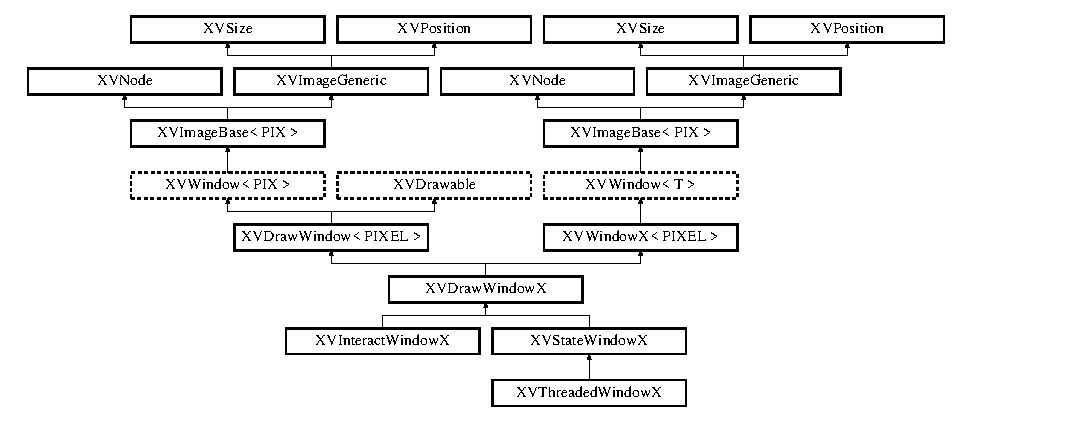
\includegraphics[height=5.23977cm]{class_XVDrawWindowX}
\end{center}
\end{figure}
\subsection*{Public Methods}
\begin{CompactItemize}
\item 
\label{XVDrawWindowX_a0}
\hypertarget{class_XVDrawWindowX_a0}{
\index{XVDrawWindowX@{XVDrawWindowX}!XVDrawWindowX@{XVDraw\-Window\-X}}\index{XVDrawWindowX@{XVDrawWindowX}!XVDrawWindowX@{XVDraw\-Window\-X}}
{\bf XVDraw\-Window\-X} (const \hyperlink{class_XVImageRGB}{XVImage\-RGB}$<$PIXEL $>$ \& im, int px = 0, int py = 0, char $\ast$ title = NULL, int event\_\-mask = 0, char $\ast$ disp = NULL, int num\_\-buf = 2, int double\_\-buf = 1, int function = GXcopy)}

\item 
\label{XVDrawWindowX_a1}
\hypertarget{class_XVDrawWindowX_a1}{
\index{XVDrawWindowX@{XVDrawWindowX}!XVDrawWindowX@{XVDraw\-Window\-X}}\index{XVDrawWindowX@{XVDrawWindowX}!XVDrawWindowX@{XVDraw\-Window\-X}}
{\bf XVDraw\-Window\-X} (int w, int h, int px = 0, int py = 0, char $\ast$ title = NULL, int event\_\-mask = 0, char $\ast$ disp = NULL, int num\_\-buf = 2, int double\_\-buf = 1, int function = GXcopy)}

\item 
\label{XVDrawWindowX_a2}
\hypertarget{class_XVDrawWindowX_a2}{
\index{~XVDrawWindowX@{$\sim$XVDrawWindowX}!XVDrawWindowX@{XVDraw\-Window\-X}}\index{XVDrawWindowX@{XVDrawWindowX}!~XVDrawWindowX@{$\sim$XVDraw\-Window\-X}}
{\bf $\sim$XVDraw\-Window\-X} ()}

\item 
void {\bf set\-XOR} ()
\item 
void {\bf set\-COPY} ()
\item 
\label{XVDrawWindowX_a5}
\hypertarget{class_XVDrawWindowX_a5}{
\index{addColor@{addColor}!XVDrawWindowX@{XVDraw\-Window\-X}}\index{XVDrawWindowX@{XVDrawWindowX}!addColor@{add\-Color}}
virtual void {\bf add\-Color} (\hyperlink{class_XVDrawColor}{XVDraw\-Color})}

\item 
\label{XVDrawWindowX_a6}
\hypertarget{class_XVDrawWindowX_a6}{
\index{drawPoint@{drawPoint}!XVDrawWindowX@{XVDraw\-Window\-X}}\index{XVDrawWindowX@{XVDrawWindowX}!drawPoint@{draw\-Point}}
virtual int {\bf draw\-Point} (int x, int y, \hyperlink{class_XVDrawColor}{XVDraw\-Color} c = DEFAULT\_\-COLOR)}

\item 
\label{XVDrawWindowX_a7}
\hypertarget{class_XVDrawWindowX_a7}{
\index{drawLine@{drawLine}!XVDrawWindowX@{XVDraw\-Window\-X}}\index{XVDrawWindowX@{XVDrawWindowX}!drawLine@{draw\-Line}}
virtual int {\bf draw\-Line} (int x1, int y1, int x2, int y2, \hyperlink{class_XVDrawColor}{XVDraw\-Color} c = DEFAULT\_\-COLOR)}

\item 
\label{XVDrawWindowX_a8}
\hypertarget{class_XVDrawWindowX_a8}{
\index{drawRectangle@{drawRectangle}!XVDrawWindowX@{XVDraw\-Window\-X}}\index{XVDrawWindowX@{XVDrawWindowX}!drawRectangle@{draw\-Rectangle}}
virtual int {\bf draw\-Rectangle} (int x, int y, int w, int h, \hyperlink{class_XVDrawColor}{XVDraw\-Color} c = DEFAULT\_\-COLOR)}

\item 
\label{XVDrawWindowX_a9}
\hypertarget{class_XVDrawWindowX_a9}{
\index{drawEllipse@{drawEllipse}!XVDrawWindowX@{XVDraw\-Window\-X}}\index{XVDrawWindowX@{XVDrawWindowX}!drawEllipse@{draw\-Ellipse}}
virtual int {\bf draw\-Ellipse} (int x, int y, int w, int h, \hyperlink{class_XVDrawColor}{XVDraw\-Color} c = DEFAULT\_\-COLOR)}

\item 
\label{XVDrawWindowX_a10}
\hypertarget{class_XVDrawWindowX_a10}{
\index{fillRectangle@{fillRectangle}!XVDrawWindowX@{XVDraw\-Window\-X}}\index{XVDrawWindowX@{XVDrawWindowX}!fillRectangle@{fill\-Rectangle}}
virtual int {\bf fill\-Rectangle} (int x, int y, int w, int h, \hyperlink{class_XVDrawColor}{XVDraw\-Color} c = DEFAULT\_\-COLOR)}

\item 
\label{XVDrawWindowX_a11}
\hypertarget{class_XVDrawWindowX_a11}{
\index{fillEllipse@{fillEllipse}!XVDrawWindowX@{XVDraw\-Window\-X}}\index{XVDrawWindowX@{XVDrawWindowX}!fillEllipse@{fill\-Ellipse}}
virtual int {\bf fill\-Ellipse} (int x, int y, int w, int h, \hyperlink{class_XVDrawColor}{XVDraw\-Color} c = DEFAULT\_\-COLOR)}

\item 
\label{XVDrawWindowX_a12}
\hypertarget{class_XVDrawWindowX_a12}{
\index{drawString@{drawString}!XVDrawWindowX@{XVDraw\-Window\-X}}\index{XVDrawWindowX@{XVDrawWindowX}!drawString@{draw\-String}}
virtual int {\bf draw\-String} (int x, int y, char $\ast$ str, int length, \hyperlink{class_XVDrawColor}{XVDraw\-Color} c = DEFAULT\_\-COLOR)}

\end{CompactItemize}
\subsection*{Protected Methods}
\begin{CompactItemize}
\item 
\label{XVDrawWindowX_b0}
\hypertarget{class_XVDrawWindowX_b0}{
\index{setFunction@{setFunction}!XVDrawWindowX@{XVDraw\-Window\-X}}\index{XVDrawWindowX@{XVDrawWindowX}!setFunction@{set\-Function}}
void {\bf set\-Function} (int)}

\end{CompactItemize}
\subsection*{Protected Attributes}
\begin{CompactItemize}
\item 
std::map$<$string, GC$>$ {\bf GCmap}
\item 
int {\bf function}
\end{CompactItemize}
\subsection*{Private Types}
\begin{CompactItemize}
\item 
typedef std::map$<$string, GCiterator {\bf MI}
\end{CompactItemize}


\subsection{Detailed Description}
\subsubsection*{template$<$class PIXEL$>$  template class XVDraw\-Window\-X}

subclass of \hyperlink{class_XVWindowX}{XVWindow\-X} that has basic shape drawing functionality.





Definition at line 436 of file XVWindow\-X.h.

\subsection{Member Typedef Documentation}
\label{XVDrawWindowX_u0}
\hypertarget{class_XVDrawWindowX_u0}{
\index{XVDrawWindowX@{XVDraw\-Window\-X}!MI@{MI}}
\index{MI@{MI}!XVDrawWindowX@{XVDraw\-Window\-X}}
\subsubsection[MI]{\setlength{\rightskip}{0pt plus 5cm}template$<$classPIXEL$>$ typedef std::map$<$string, GC$>$::iterator XVDraw\-Window\-X$<$PIXEL$>$::MI\hspace{0.3cm}{\tt  \mbox{[}private\mbox{]}}}}




Definition at line 439 of file XVWindow\-X.h.

\subsection{Member Function Documentation}
\label{XVDrawWindowX_a3}
\hypertarget{class_XVDrawWindowX_a3}{
\index{XVDrawWindowX@{XVDraw\-Window\-X}!setXOR@{setXOR}}
\index{setXOR@{setXOR}!XVDrawWindowX@{XVDraw\-Window\-X}}
\subsubsection[setXOR]{\setlength{\rightskip}{0pt plus 5cm}template$<$classPIXEL$>$ void XVDraw\-Window\-X$<$PIXEL$>$::set\-XOR ()\hspace{0.3cm}{\tt  \mbox{[}inline, virtual\mbox{]}}}}




Reimplemented from \hyperlink{class_XVDrawable}{XVDrawable}.

Definition at line 482 of file XVWindow\-X.h.\label{XVDrawWindowX_a4}
\hypertarget{class_XVDrawWindowX_a4}{
\index{XVDrawWindowX@{XVDraw\-Window\-X}!setCOPY@{setCOPY}}
\index{setCOPY@{setCOPY}!XVDrawWindowX@{XVDraw\-Window\-X}}
\subsubsection[setCOPY]{\setlength{\rightskip}{0pt plus 5cm}template$<$classPIXEL$>$ void XVDraw\-Window\-X$<$PIXEL$>$::set\-COPY ()\hspace{0.3cm}{\tt  \mbox{[}inline, virtual\mbox{]}}}}




Reimplemented from \hyperlink{class_XVDrawable}{XVDrawable}.

Definition at line 483 of file XVWindow\-X.h.

\subsection{Member Data Documentation}
\label{XVDrawWindowX_n0}
\hypertarget{class_XVDrawWindowX_n0}{
\index{XVDrawWindowX@{XVDraw\-Window\-X}!GCmap@{GCmap}}
\index{GCmap@{GCmap}!XVDrawWindowX@{XVDraw\-Window\-X}}
\subsubsection[GCmap]{\setlength{\rightskip}{0pt plus 5cm}template$<$classPIXEL$>$ std::map$<$ string,GC $>$ XVDraw\-Window\-X$<$PIXEL$>$::GCmap\hspace{0.3cm}{\tt  \mbox{[}protected\mbox{]}}}}




Definition at line 463 of file XVWindow\-X.h.\label{XVDrawWindowX_n1}
\hypertarget{class_XVDrawWindowX_n1}{
\index{XVDrawWindowX@{XVDraw\-Window\-X}!function@{function}}
\index{function@{function}!XVDrawWindowX@{XVDraw\-Window\-X}}
\subsubsection[function]{\setlength{\rightskip}{0pt plus 5cm}template$<$classPIXEL$>$ int XVDraw\-Window\-X$<$PIXEL$>$::function\hspace{0.3cm}{\tt  \mbox{[}protected\mbox{]}}}}




Definition at line 464 of file XVWindow\-X.h.

The documentation for this class was generated from the following file:\begin{CompactItemize}
\item 
/home/burschka/XVision2-2.0.0/src/Consoles/\hyperlink{XVWindowX.h-source}{XVWindow\-X.h}\end{CompactItemize}

\hypertarget{class_XVEdge}{
\section{XVEdge  Template Class Reference}
\label{XVEdge}\index{XVEdge@{XVEdge}}
}
XVEdge class declaration This is a simple, fast, signed edge with a -1, 1 mask. 


{\tt \#include $<$XVPattern.h$>$}

Inheritance diagram for XVEdge:\begin{figure}[H]
\begin{center}
\leavevmode
\includegraphics[height=2cm]{class_XVEdge}
\end{center}
\end{figure}
\subsection*{Public Methods}
\begin{CompactItemize}
\item 
{\bf XVEdge} (int mwidth\_\-in = default\_\-mwidth, float alpha\_\-in = default\_\-alpha)
\item 
{\bf XVEdge} (const XVEdge \& e)
\item 
virtual \hyperlink{class_XVPattern}{XVPattern}$<$T$>$$\ast$ {\bf dup} ()
\item 
int {\bf xpad} (int , int height)
\item 
int {\bf ypad} (int , int )
\item 
\label{XVEdge_a5}
\hypertarget{class_XVEdge_a5}{
\index{find@{find}!XVEdge@{XVEdge}}\index{XVEdge@{XVEdge}!find@{find}}
XVOffset {\bf find} (\hyperlink{class_XVImageScalar}{XVImage\-Scalar}$<$T$>$ \&)}

\item 
linetype\& {\bf line\-Type} ()
\end{CompactItemize}
\subsection*{Private Attributes}
\begin{CompactItemize}
\item 
float {\bf alpha}
\item 
linetype {\bf trans\_\-type}
\end{CompactItemize}


\subsection{Detailed Description}
\subsubsection*{template$<$class T$>$  template class XVEdge}

XVEdge class declaration This is a simple, fast, signed edge with a -1, 1 mask.





Definition at line 129 of file XVPattern.h.

\subsection{Constructor \& Destructor Documentation}
\label{XVEdge_a0}
\hypertarget{class_XVEdge_a0}{
\index{XVEdge@{XVEdge}!XVEdge@{XVEdge}}
\index{XVEdge@{XVEdge}!XVEdge@{XVEdge}}
\subsubsection[XVEdge]{\setlength{\rightskip}{0pt plus 5cm}template$<$classT$>$ XVEdge$<$T$>$::XVEdge$<$T$>$ (int {\em mwidth\_\-in} = default\_\-mwidth, float {\em alpha\_\-in} = default\_\-alpha)\hspace{0.3cm}{\tt  \mbox{[}inline\mbox{]}}}}




Definition at line 147 of file XVPattern.h.\label{XVEdge_a1}
\hypertarget{class_XVEdge_a1}{
\index{XVEdge@{XVEdge}!XVEdge@{XVEdge}}
\index{XVEdge@{XVEdge}!XVEdge@{XVEdge}}
\subsubsection[XVEdge]{\setlength{\rightskip}{0pt plus 5cm}template$<$classT$>$ XVEdge$<$T$>$::XVEdge$<$T$>$ (const XVEdge$<$T$>$ \& {\em e})\hspace{0.3cm}{\tt  \mbox{[}inline\mbox{]}}}}




Definition at line 156 of file XVPattern.h.

\subsection{Member Function Documentation}
\label{XVEdge_a2}
\hypertarget{class_XVEdge_a2}{
\index{XVEdge@{XVEdge}!dup@{dup}}
\index{dup@{dup}!XVEdge@{XVEdge}}
\subsubsection[dup]{\setlength{\rightskip}{0pt plus 5cm}template$<$classT$>$ \hyperlink{class_XVPattern}{XVPattern}$<$ T $>$$\ast$ XVEdge$<$T$>$::dup$<$T$>$ ()\hspace{0.3cm}{\tt  \mbox{[}inline, virtual\mbox{]}}}}




Definition at line 158 of file XVPattern.h.\label{XVEdge_a3}
\hypertarget{class_XVEdge_a3}{
\index{XVEdge@{XVEdge}!xpad@{xpad}}
\index{xpad@{xpad}!XVEdge@{XVEdge}}
\subsubsection[xpad]{\setlength{\rightskip}{0pt plus 5cm}template$<$classT$>$ int XVEdge$<$T$>$::xpad (int {\em width}, int {\em height})\hspace{0.3cm}{\tt  \mbox{[}inline, virtual\mbox{]}}}}




Reimplemented from \hyperlink{class_XVPattern}{XVPattern}.

Definition at line 160 of file XVPattern.h.\label{XVEdge_a4}
\hypertarget{class_XVEdge_a4}{
\index{XVEdge@{XVEdge}!ypad@{ypad}}
\index{ypad@{ypad}!XVEdge@{XVEdge}}
\subsubsection[ypad]{\setlength{\rightskip}{0pt plus 5cm}template$<$classT$>$ int XVEdge$<$T$>$::ypad (int {\em width}, int {\em height})\hspace{0.3cm}{\tt  \mbox{[}inline, virtual\mbox{]}}}}




Reimplemented from \hyperlink{class_XVPattern}{XVPattern}.

Definition at line 162 of file XVPattern.h.\label{XVEdge_a6}
\hypertarget{class_XVEdge_a6}{
\index{XVEdge@{XVEdge}!lineType@{lineType}}
\index{lineType@{lineType}!XVEdge@{XVEdge}}
\subsubsection[lineType]{\setlength{\rightskip}{0pt plus 5cm}template$<$classT$>$ linetype \& XVEdge$<$T$>$::line\-Type ()\hspace{0.3cm}{\tt  \mbox{[}inline\mbox{]}}}}




Definition at line 166 of file XVPattern.h.

\subsection{Member Data Documentation}
\label{XVEdge_o0}
\hypertarget{class_XVEdge_o0}{
\index{XVEdge@{XVEdge}!alpha@{alpha}}
\index{alpha@{alpha}!XVEdge@{XVEdge}}
\subsubsection[alpha]{\setlength{\rightskip}{0pt plus 5cm}template$<$classT$>$ float XVEdge$<$T$>$::alpha\hspace{0.3cm}{\tt  \mbox{[}private\mbox{]}}}}




Definition at line 137 of file XVPattern.h.\label{XVEdge_o1}
\hypertarget{class_XVEdge_o1}{
\index{XVEdge@{XVEdge}!trans_type@{trans\_\-type}}
\index{trans_type@{trans\_\-type}!XVEdge@{XVEdge}}
\subsubsection[trans_type]{\setlength{\rightskip}{0pt plus 5cm}template$<$classT$>$ linetype XVEdge$<$T$>$::trans\_\-type\hspace{0.3cm}{\tt  \mbox{[}private\mbox{]}}}}




Definition at line 143 of file XVPattern.h.

The documentation for this class was generated from the following file:\begin{CompactItemize}
\item 
/home/burschka/XVision2-2.0.0/src/Tracking/Edges/\hyperlink{XVPattern.h-source}{XVPattern.h}\end{CompactItemize}

\hypertarget{class_XVException}{
\section{XVException  Class Reference}
\label{XVException}\index{XVException@{XVException}}
}
base class for an XVision exception. 


{\tt \#include $<$XVException.h$>$}

Inheritance diagram for XVException:\begin{figure}[H]
\begin{center}
\leavevmode
\includegraphics[height=11cm]{class_XVException}
\end{center}
\end{figure}
\subsection*{Public Methods}
\begin{CompactItemize}
\item 
{\bf XVException} ()
\item 
{\bf XVException} (char $\ast$ err)
\item 
const char$\ast$ {\bf what} () const  throw ()
\end{CompactItemize}
\subsection*{Protected Attributes}
\begin{CompactItemize}
\item 
char$\ast$ {\bf error}
\end{CompactItemize}


\subsection{Detailed Description}
base class for an XVision exception.





Definition at line 9 of file XVException.h.

\subsection{Constructor \& Destructor Documentation}
\label{XVException_a0}
\hypertarget{class_XVException_a0}{
\index{XVException@{XVException}!XVException@{XVException}}
\index{XVException@{XVException}!XVException@{XVException}}
\subsubsection[XVException]{\setlength{\rightskip}{0pt plus 5cm}XVException::XVException ()\hspace{0.3cm}{\tt  \mbox{[}inline\mbox{]}}}}




Definition at line 17 of file XVException.h.\label{XVException_a1}
\hypertarget{class_XVException_a1}{
\index{XVException@{XVException}!XVException@{XVException}}
\index{XVException@{XVException}!XVException@{XVException}}
\subsubsection[XVException]{\setlength{\rightskip}{0pt plus 5cm}XVException::XVException (char $\ast$ {\em err})\hspace{0.3cm}{\tt  \mbox{[}inline\mbox{]}}}}




Definition at line 18 of file XVException.h.

\subsection{Member Function Documentation}
\label{XVException_a2}
\hypertarget{class_XVException_a2}{
\index{XVException@{XVException}!what@{what}}
\index{what@{what}!XVException@{XVException}}
\subsubsection[what]{\setlength{\rightskip}{0pt plus 5cm}const char $\ast$ XVException::what () const  throw ()\hspace{0.3cm}{\tt  \mbox{[}inline\mbox{]}}}}




Definition at line 20 of file XVException.h.

\subsection{Member Data Documentation}
\label{XVException_n0}
\hypertarget{class_XVException_n0}{
\index{XVException@{XVException}!error@{error}}
\index{error@{error}!XVException@{XVException}}
\subsubsection[error]{\setlength{\rightskip}{0pt plus 5cm}char $\ast$ XVException::error\hspace{0.3cm}{\tt  \mbox{[}protected\mbox{]}}}}




Definition at line 13 of file XVException.h.

The documentation for this class was generated from the following file:\begin{CompactItemize}
\item 
/home/burschka/XVision2-2.0.0/src/Tools/\hyperlink{XVException.h-source}{XVException.h}\end{CompactItemize}

\hypertarget{class_XVGroupTracker}{
\section{XVGroup\-Tracker  Template Class Reference}
\label{XVGroupTracker}\index{XVGroupTracker@{XVGroup\-Tracker}}
}
XVGroup\-Tracker. 


{\tt \#include $<$XVGroup\-Tracker.h$>$}

Inheritance diagram for XVGroup\-Tracker:\begin{figure}[H]
\begin{center}
\leavevmode
\includegraphics[height=2cm]{class_XVGroupTracker}
\end{center}
\end{figure}
\subsection*{Public Types}
\begin{CompactItemize}
\item 
typedef FEATURETYPE::STATE {\bf STATE}
\end{CompactItemize}
\subsection*{Public Methods}
\begin{CompactItemize}
\item 
{\bf XVGroup\-Tracker} (SRCTYPE \& s, FEATURETYPE \& f, int pf = DEFAULT\_\-ITERATIONS)
\item 
virtual vector$<$STATE $>$ {\bf init} (vector$<$STATE $>$ \& init\-States)
\item 
virtual void {\bf track} ()  throw (XVTracker\-Exception)
\item 
virtual vector$<$STATE $>$ {\bf next\-State} ()  throw (XVTracker\-Exception)
\item 
void {\bf add\-Feature} (FEATURETYPE \& f)
\item 
void {\bf remove\-Feature} (int i)
\item 
vector$<$FEATURETYPE $\ast$$>$\& {\bf get\-Features} ()
\end{CompactItemize}
\subsection*{Protected Attributes}
\begin{CompactItemize}
\item 
SRCTYPE\& {\bf source}
\item 
vector$<$FEATURETYPE $\ast$$>$ {\bf features}
\item 
int {\bf steps\-Per\-Frame}
\item 
int {\bf frame\-Num}
\end{CompactItemize}


\subsection{Detailed Description}
\subsubsection*{template$<$class SRCTYPE, class FEATURETYPE$>$  template class XVGroup\-Tracker}

XVGroup\-Tracker.

\begin{Desc}
\item[{\bf Author(s): }]\par
 Sam Lang \end{Desc}
\begin{Desc}
\item[{\bf Version: }]\par
 \end{Desc}
\begin{Desc}
\item[{\bf Id: }] XVGroup\-Tracker.h,v 1.6 2005/02/22 02:35:54 cvsuser Exp \end{Desc}


XVGroup\-Tracker is just like \hyperlink{class_XVTracker}{XVTracker}, except you can have multiple features.

\begin{Desc}
\item[{\bf See also: }]\par
 \hyperlink{class_XVTracker}{XVTracker} ,  \hyperlink{class_XVVideo}{XVVideo} ,  XVFeature \end{Desc}




Definition at line 37 of file XVGroup\-Tracker.h.

\subsection{Member Typedef Documentation}
\label{XVGroupTracker_s0}
\hypertarget{class_XVGroupTracker_s0}{
\index{XVGroupTracker@{XVGroup\-Tracker}!STATE@{STATE}}
\index{STATE@{STATE}!XVGroupTracker@{XVGroup\-Tracker}}
\subsubsection[STATE]{\setlength{\rightskip}{0pt plus 5cm}template$<$classSRCTYPE, classFEATURETYPE$>$ typedef FEATURETYPE::STATE XVGroup\-Tracker$<$SRCTYPE, FEATURETYPE$>$::STATE}}




Definition at line 49 of file XVGroup\-Tracker.h.

\subsection{Constructor \& Destructor Documentation}
\label{XVGroupTracker_a0}
\hypertarget{class_XVGroupTracker_a0}{
\index{XVGroupTracker@{XVGroup\-Tracker}!XVGroupTracker@{XVGroupTracker}}
\index{XVGroupTracker@{XVGroupTracker}!XVGroupTracker@{XVGroup\-Tracker}}
\subsubsection[XVGroupTracker]{\setlength{\rightskip}{0pt plus 5cm}template$<$classSRCTYPE, classFEATURETYPE$>$ XVGroup\-Tracker$<$SRCTYPE, FEATURETYPE$>$::XVGroup\-Tracker$<$SRCTYPE, FEATURETYPE$>$ (SRCTYPE \& {\em s}, FEATURETYPE \& {\em f}, int {\em pf} = DEFAULT\_\-ITERATIONS)}}




Definition at line 51 of file XVGroup\-Tracker.h.

\subsection{Member Function Documentation}
\label{XVGroupTracker_a1}
\hypertarget{class_XVGroupTracker_a1}{
\index{XVGroupTracker@{XVGroup\-Tracker}!init@{init}}
\index{init@{init}!XVGroupTracker@{XVGroup\-Tracker}}
\subsubsection[init]{\setlength{\rightskip}{0pt plus 5cm}template$<$classSRCTYPE, classFEATURETYPE$>$ vector$<$ STATE $>$ XVGroup\-Tracker$<$SRCTYPE, FEATURETYPE$>$::init$<$STATE $>$ (vector$<$ STATE $>$\& {\em init\-States})\hspace{0.3cm}{\tt  \mbox{[}inline, virtual\mbox{]}}}}




Definition at line 54 of file XVGroup\-Tracker.h.\label{XVGroupTracker_a2}
\hypertarget{class_XVGroupTracker_a2}{
\index{XVGroupTracker@{XVGroup\-Tracker}!track@{track}}
\index{track@{track}!XVGroupTracker@{XVGroup\-Tracker}}
\subsubsection[track]{\setlength{\rightskip}{0pt plus 5cm}template$<$classSRC, classFEATURE$>$ void XVGroup\-Tracker$<$ SRC,FEATURE $>$::track ()  throw (\hyperlink{class_XVTrackerException}{XVTracker\-Exception})\hspace{0.3cm}{\tt  \mbox{[}virtual\mbox{]}}}}




Definition at line 24 of file XVGroup\-Tracker.icc.\label{XVGroupTracker_a3}
\hypertarget{class_XVGroupTracker_a3}{
\index{XVGroupTracker@{XVGroup\-Tracker}!nextState@{nextState}}
\index{nextState@{nextState}!XVGroupTracker@{XVGroup\-Tracker}}
\subsubsection[nextState]{\setlength{\rightskip}{0pt plus 5cm}template$<$classSRC, classFEATURE$>$ vector$<$ typename FEATURE::STATE $>$ XVGroup\-Tracker$<$ SRC,FEATURE $>$::next\-State ()  throw (\hyperlink{class_XVTrackerException}{XVTracker\-Exception})\hspace{0.3cm}{\tt  \mbox{[}virtual\mbox{]}}}}




Definition at line 9 of file XVGroup\-Tracker.icc.\label{XVGroupTracker_a4}
\hypertarget{class_XVGroupTracker_a4}{
\index{XVGroupTracker@{XVGroup\-Tracker}!addFeature@{addFeature}}
\index{addFeature@{addFeature}!XVGroupTracker@{XVGroup\-Tracker}}
\subsubsection[addFeature]{\setlength{\rightskip}{0pt plus 5cm}template$<$classSRCTYPE, classFEATURETYPE$>$ void XVGroup\-Tracker$<$SRCTYPE, FEATURETYPE$>$::add\-Feature (FEATURETYPE \& {\em f})\hspace{0.3cm}{\tt  \mbox{[}inline\mbox{]}}}}




Definition at line 65 of file XVGroup\-Tracker.h.\label{XVGroupTracker_a5}
\hypertarget{class_XVGroupTracker_a5}{
\index{XVGroupTracker@{XVGroup\-Tracker}!removeFeature@{removeFeature}}
\index{removeFeature@{removeFeature}!XVGroupTracker@{XVGroup\-Tracker}}
\subsubsection[removeFeature]{\setlength{\rightskip}{0pt plus 5cm}template$<$classSRCTYPE, classFEATURETYPE$>$ void XVGroup\-Tracker$<$SRCTYPE, FEATURETYPE$>$::remove\-Feature (int {\em i})\hspace{0.3cm}{\tt  \mbox{[}inline\mbox{]}}}}




Definition at line 66 of file XVGroup\-Tracker.h.\label{XVGroupTracker_a6}
\hypertarget{class_XVGroupTracker_a6}{
\index{XVGroupTracker@{XVGroup\-Tracker}!getFeatures@{getFeatures}}
\index{getFeatures@{getFeatures}!XVGroupTracker@{XVGroup\-Tracker}}
\subsubsection[getFeatures]{\setlength{\rightskip}{0pt plus 5cm}template$<$classSRCTYPE, classFEATURETYPE$>$ vector$<$ FEATURETYPE $\ast$$>$\& XVGroup\-Tracker$<$SRCTYPE, FEATURETYPE$>$::get\-Features$<$FEATURETYPE $\ast$$>$ ()\hspace{0.3cm}{\tt  \mbox{[}inline\mbox{]}}}}




Definition at line 67 of file XVGroup\-Tracker.h.

\subsection{Member Data Documentation}
\label{XVGroupTracker_n0}
\hypertarget{class_XVGroupTracker_n0}{
\index{XVGroupTracker@{XVGroup\-Tracker}!source@{source}}
\index{source@{source}!XVGroupTracker@{XVGroup\-Tracker}}
\subsubsection[source]{\setlength{\rightskip}{0pt plus 5cm}template$<$classSRCTYPE, classFEATURETYPE$>$ SRCTYPE \& XVGroup\-Tracker$<$SRCTYPE, FEATURETYPE$>$::source\hspace{0.3cm}{\tt  \mbox{[}protected\mbox{]}}}}




Definition at line 41 of file XVGroup\-Tracker.h.\label{XVGroupTracker_n1}
\hypertarget{class_XVGroupTracker_n1}{
\index{XVGroupTracker@{XVGroup\-Tracker}!features@{features}}
\index{features@{features}!XVGroupTracker@{XVGroup\-Tracker}}
\subsubsection[features]{\setlength{\rightskip}{0pt plus 5cm}template$<$classSRCTYPE, classFEATURETYPE$>$ vector$<$ FEATURETYPE $\ast$$>$ XVGroup\-Tracker$<$SRCTYPE, FEATURETYPE$>$::features\hspace{0.3cm}{\tt  \mbox{[}protected\mbox{]}}}}




Definition at line 42 of file XVGroup\-Tracker.h.\label{XVGroupTracker_n2}
\hypertarget{class_XVGroupTracker_n2}{
\index{XVGroupTracker@{XVGroup\-Tracker}!stepsPerFrame@{stepsPerFrame}}
\index{stepsPerFrame@{stepsPerFrame}!XVGroupTracker@{XVGroup\-Tracker}}
\subsubsection[stepsPerFrame]{\setlength{\rightskip}{0pt plus 5cm}template$<$classSRCTYPE, classFEATURETYPE$>$ int XVGroup\-Tracker$<$SRCTYPE, FEATURETYPE$>$::steps\-Per\-Frame\hspace{0.3cm}{\tt  \mbox{[}protected\mbox{]}}}}




Definition at line 44 of file XVGroup\-Tracker.h.\label{XVGroupTracker_n3}
\hypertarget{class_XVGroupTracker_n3}{
\index{XVGroupTracker@{XVGroup\-Tracker}!frameNum@{frameNum}}
\index{frameNum@{frameNum}!XVGroupTracker@{XVGroup\-Tracker}}
\subsubsection[frameNum]{\setlength{\rightskip}{0pt plus 5cm}template$<$classSRCTYPE, classFEATURETYPE$>$ int XVGroup\-Tracker$<$SRCTYPE, FEATURETYPE$>$::frame\-Num\hspace{0.3cm}{\tt  \mbox{[}protected\mbox{]}}}}




Definition at line 45 of file XVGroup\-Tracker.h.

The documentation for this class was generated from the following files:\begin{CompactItemize}
\item 
/home/burschka/XVision2-2.0.0/src/Tracking/\hyperlink{XVGroupTracker.h-source}{XVGroup\-Tracker.h}\item 
/home/burschka/XVision2-2.0.0/src/Tracking/\hyperlink{XVGroupTracker.icc-source}{XVGroup\-Tracker.icc}\end{CompactItemize}

\hypertarget{class_XVHueRangeTable}{
\section{XVHue\-Range\-Table  Template Class Reference}
\label{XVHueRangeTable}\index{XVHueRangeTable@{XVHue\-Range\-Table}}
}
The Hue\-Range\-Table class allows for fast lookup to find the hue of a given RGB value The table holds boolean values: true if the hue of the RGB pixel was within the desired range, false otherwise. 


{\tt \#include $<$XVColor\-Seg.h$>$}

Inheritance diagram for XVHue\-Range\-Table:\begin{figure}[H]
\begin{center}
\leavevmode
\includegraphics[height=3cm]{class_XVHueRangeTable}
\end{center}
\end{figure}
\subsection*{Public Methods}
\begin{CompactItemize}
\item 
{\bf XVHue\-Range\-Table} (HUERANGE range, u\_\-char dp, u\_\-char bp)
\item 
{\bf $\sim$XVHue\-Range\-Table} ()
\item 
\label{XVHueRangeTable_a2}
\hypertarget{class_XVHueRangeTable_a2}{
\index{updateTable@{updateTable}!XVHueRangeTable@{XVHue\-Range\-Table}}\index{XVHueRangeTable@{XVHueRangeTable}!updateTable@{update\-Table}}
void {\bf update\-Table} (HUERANGE)}

\item 
HUERANGE {\bf get\-Range} ()
\end{CompactItemize}
\subsection*{Public Attributes}
\begin{CompactItemize}
\item 
HUERANGE {\bf hue\-Range}
\item 
\hyperlink{class_XVHueSectorTable}{XVHue\-Sector\-Table}$<$T, Y$>$$\ast$ {\bf hue\-Table}
\end{CompactItemize}
\subsection*{Protected Methods}
\begin{CompactItemize}
\item 
\label{XVHueRangeTable_b0}
\hypertarget{class_XVHueRangeTable_b0}{
\index{computeValue@{computeValue}!XVHueRangeTable@{XVHue\-Range\-Table}}\index{XVHueRangeTable@{XVHueRangeTable}!computeValue@{compute\-Value}}
Y {\bf compute\-Value} (T)}

\end{CompactItemize}
\subsection*{Protected Attributes}
\begin{CompactItemize}
\item 
u\_\-char {\bf dark\-Pix}
\item 
u\_\-char {\bf bright\-Pix}
\end{CompactItemize}


\subsection{Detailed Description}
\subsubsection*{template$<$class T, class Y$>$  template class XVHue\-Range\-Table}

The Hue\-Range\-Table class allows for fast lookup to find the hue of a given RGB value The table holds boolean values: true if the hue of the RGB pixel was within the desired range, false otherwise.





Definition at line 170 of file XVColor\-Seg.h.

\subsection{Constructor \& Destructor Documentation}
\label{XVHueRangeTable_a0}
\hypertarget{class_XVHueRangeTable_a0}{
\index{XVHueRangeTable@{XVHue\-Range\-Table}!XVHueRangeTable@{XVHueRangeTable}}
\index{XVHueRangeTable@{XVHueRangeTable}!XVHueRangeTable@{XVHue\-Range\-Table}}
\subsubsection[XVHueRangeTable]{\setlength{\rightskip}{0pt plus 5cm}template$<$classT, classY$>$ XVHue\-Range\-Table$<$T, Y$>$::XVHue\-Range\-Table$<$T, Y$>$ (HUERANGE {\em range}, u\_\-char {\em dp}, u\_\-char {\em bp})}}




Definition at line 183 of file XVColor\-Seg.h.\label{XVHueRangeTable_a1}
\hypertarget{class_XVHueRangeTable_a1}{
\index{XVHueRangeTable@{XVHue\-Range\-Table}!~XVHueRangeTable@{$\sim$XVHueRangeTable}}
\index{~XVHueRangeTable@{$\sim$XVHueRangeTable}!XVHueRangeTable@{XVHue\-Range\-Table}}
\subsubsection[~XVHueRangeTable]{\setlength{\rightskip}{0pt plus 5cm}template$<$classT, classY$>$ XVHue\-Range\-Table$<$T, Y$>$::$\sim$XVHue\-Range\-Table$<$T, Y$>$ ()\hspace{0.3cm}{\tt  \mbox{[}inline\mbox{]}}}}




Definition at line 189 of file XVColor\-Seg.h.

\subsection{Member Function Documentation}
\label{XVHueRangeTable_a3}
\hypertarget{class_XVHueRangeTable_a3}{
\index{XVHueRangeTable@{XVHue\-Range\-Table}!getRange@{getRange}}
\index{getRange@{getRange}!XVHueRangeTable@{XVHue\-Range\-Table}}
\subsubsection[getRange]{\setlength{\rightskip}{0pt plus 5cm}template$<$classT, classY$>$ HUERANGE XVHue\-Range\-Table$<$T, Y$>$::get\-Range ()\hspace{0.3cm}{\tt  \mbox{[}inline\mbox{]}}}}




Definition at line 192 of file XVColor\-Seg.h.

\subsection{Member Data Documentation}
\label{XVHueRangeTable_n0}
\hypertarget{class_XVHueRangeTable_n0}{
\index{XVHueRangeTable@{XVHue\-Range\-Table}!darkPix@{darkPix}}
\index{darkPix@{darkPix}!XVHueRangeTable@{XVHue\-Range\-Table}}
\subsubsection[darkPix]{\setlength{\rightskip}{0pt plus 5cm}template$<$classT, classY$>$ u\_\-char XVHue\-Range\-Table$<$T, Y$>$::dark\-Pix\hspace{0.3cm}{\tt  \mbox{[}protected\mbox{]}}}}




Definition at line 175 of file XVColor\-Seg.h.\label{XVHueRangeTable_n1}
\hypertarget{class_XVHueRangeTable_n1}{
\index{XVHueRangeTable@{XVHue\-Range\-Table}!brightPix@{brightPix}}
\index{brightPix@{brightPix}!XVHueRangeTable@{XVHue\-Range\-Table}}
\subsubsection[brightPix]{\setlength{\rightskip}{0pt plus 5cm}template$<$classT, classY$>$ u\_\-char XVHue\-Range\-Table$<$T, Y$>$::bright\-Pix\hspace{0.3cm}{\tt  \mbox{[}protected\mbox{]}}}}




Definition at line 175 of file XVColor\-Seg.h.\label{XVHueRangeTable_m0}
\hypertarget{class_XVHueRangeTable_m0}{
\index{XVHueRangeTable@{XVHue\-Range\-Table}!hueRange@{hueRange}}
\index{hueRange@{hueRange}!XVHueRangeTable@{XVHue\-Range\-Table}}
\subsubsection[hueRange]{\setlength{\rightskip}{0pt plus 5cm}template$<$classT, classY$>$ HUERANGE XVHue\-Range\-Table$<$T, Y$>$::hue\-Range}}




Definition at line 179 of file XVColor\-Seg.h.\label{XVHueRangeTable_m1}
\hypertarget{class_XVHueRangeTable_m1}{
\index{XVHueRangeTable@{XVHue\-Range\-Table}!hueTable@{hueTable}}
\index{hueTable@{hueTable}!XVHueRangeTable@{XVHue\-Range\-Table}}
\subsubsection[hueTable]{\setlength{\rightskip}{0pt plus 5cm}template$<$classT, classY$>$ \hyperlink{class_XVHueSectorTable}{XVHue\-Sector\-Table}$<$ T,Y $>$$\ast$ XVHue\-Range\-Table$<$T, Y$>$::hue\-Table}}




Definition at line 181 of file XVColor\-Seg.h.

The documentation for this class was generated from the following file:\begin{CompactItemize}
\item 
/home/burschka/XVision2-2.0.0/src/Segmentation/\hyperlink{XVColorSeg.h-source}{XVColor\-Seg.h}\end{CompactItemize}

\hypertarget{class_XVHueSectorTable}{
\section{XVHue\-Sector\-Table  Template Class Reference}
\label{XVHueSectorTable}\index{XVHueSectorTable@{XVHue\-Sector\-Table}}
}
The Hue\-Sector\-Table class builds a table of the RGB to Sector (Hue Sector) values. 


{\tt \#include $<$XVColor\-Seg.h$>$}

Inheritance diagram for XVHue\-Sector\-Table:\begin{figure}[H]
\begin{center}
\leavevmode
\includegraphics[height=3cm]{class_XVHueSectorTable}
\end{center}
\end{figure}
\subsection*{Public Methods}
\begin{CompactItemize}
\item 
{\bf XVHue\-Sector\-Table} (int num, u\_\-char dp, u\_\-char bp)
\item 
int {\bf get\-Sectors} ()
\end{CompactItemize}
\subsection*{Protected Methods}
\begin{CompactItemize}
\item 
\label{XVHueSectorTable_b0}
\hypertarget{class_XVHueSectorTable_b0}{
\index{computeValue@{computeValue}!XVHueSectorTable@{XVHue\-Sector\-Table}}\index{XVHueSectorTable@{XVHueSectorTable}!computeValue@{compute\-Value}}
Y {\bf compute\-Value} (T)}

\end{CompactItemize}
\subsection*{Protected Attributes}
\begin{CompactItemize}
\item 
u\_\-char {\bf dark\-Pix}
\item 
u\_\-char {\bf bright\-Pix}
\item 
int {\bf num\-Of\-Sectors}
\end{CompactItemize}


\subsection{Detailed Description}
\subsubsection*{template$<$class T, class Y$>$  template class XVHue\-Sector\-Table}

The Hue\-Sector\-Table class builds a table of the RGB to Sector (Hue Sector) values.





Definition at line 51 of file XVColor\-Seg.h.

\subsection{Constructor \& Destructor Documentation}
\label{XVHueSectorTable_a0}
\hypertarget{class_XVHueSectorTable_a0}{
\index{XVHueSectorTable@{XVHue\-Sector\-Table}!XVHueSectorTable@{XVHueSectorTable}}
\index{XVHueSectorTable@{XVHueSectorTable}!XVHueSectorTable@{XVHue\-Sector\-Table}}
\subsubsection[XVHueSectorTable]{\setlength{\rightskip}{0pt plus 5cm}template$<$classT, classY$>$ XVHue\-Sector\-Table$<$T, Y$>$::XVHue\-Sector\-Table$<$T, Y$>$ (int {\em num}, u\_\-char {\em dp}, u\_\-char {\em bp})}}




Definition at line 63 of file XVColor\-Seg.h.

\subsection{Member Function Documentation}
\label{XVHueSectorTable_a1}
\hypertarget{class_XVHueSectorTable_a1}{
\index{XVHueSectorTable@{XVHue\-Sector\-Table}!getSectors@{getSectors}}
\index{getSectors@{getSectors}!XVHueSectorTable@{XVHue\-Sector\-Table}}
\subsubsection[getSectors]{\setlength{\rightskip}{0pt plus 5cm}template$<$classT, classY$>$ int XVHue\-Sector\-Table$<$T, Y$>$::get\-Sectors ()\hspace{0.3cm}{\tt  \mbox{[}inline\mbox{]}}}}




Definition at line 70 of file XVColor\-Seg.h.

\subsection{Member Data Documentation}
\label{XVHueSectorTable_n0}
\hypertarget{class_XVHueSectorTable_n0}{
\index{XVHueSectorTable@{XVHue\-Sector\-Table}!darkPix@{darkPix}}
\index{darkPix@{darkPix}!XVHueSectorTable@{XVHue\-Sector\-Table}}
\subsubsection[darkPix]{\setlength{\rightskip}{0pt plus 5cm}template$<$classT, classY$>$ u\_\-char XVHue\-Sector\-Table$<$T, Y$>$::dark\-Pix\hspace{0.3cm}{\tt  \mbox{[}protected\mbox{]}}}}




Definition at line 55 of file XVColor\-Seg.h.\label{XVHueSectorTable_n1}
\hypertarget{class_XVHueSectorTable_n1}{
\index{XVHueSectorTable@{XVHue\-Sector\-Table}!brightPix@{brightPix}}
\index{brightPix@{brightPix}!XVHueSectorTable@{XVHue\-Sector\-Table}}
\subsubsection[brightPix]{\setlength{\rightskip}{0pt plus 5cm}template$<$classT, classY$>$ u\_\-char XVHue\-Sector\-Table$<$T, Y$>$::bright\-Pix\hspace{0.3cm}{\tt  \mbox{[}protected\mbox{]}}}}




Definition at line 55 of file XVColor\-Seg.h.\label{XVHueSectorTable_n2}
\hypertarget{class_XVHueSectorTable_n2}{
\index{XVHueSectorTable@{XVHue\-Sector\-Table}!numOfSectors@{numOfSectors}}
\index{numOfSectors@{numOfSectors}!XVHueSectorTable@{XVHue\-Sector\-Table}}
\subsubsection[numOfSectors]{\setlength{\rightskip}{0pt plus 5cm}template$<$classT, classY$>$ int XVHue\-Sector\-Table$<$T, Y$>$::num\-Of\-Sectors\hspace{0.3cm}{\tt  \mbox{[}protected\mbox{]}}}}




Definition at line 57 of file XVColor\-Seg.h.

The documentation for this class was generated from the following file:\begin{CompactItemize}
\item 
/home/burschka/XVision2-2.0.0/src/Segmentation/\hyperlink{XVColorSeg.h-source}{XVColor\-Seg.h}\end{CompactItemize}

\hypertarget{class_XVHueSeg}{
\section{XVHue\-Seg  Template Class Reference}
\label{XVHueSeg}\index{XVHueSeg@{XVHue\-Seg}}
}
The XVHue\-Sector\-Seg class does Segmentation based on the Hue Sectors of the image. 


{\tt \#include $<$XVColor\-Seg.h$>$}

Inheritance diagram for XVHue\-Seg:\begin{figure}[H]
\begin{center}
\leavevmode
\includegraphics[height=2cm]{class_XVHueSeg}
\end{center}
\end{figure}
\subsection*{Public Methods}
\begin{CompactItemize}
\item 
\label{XVHueSeg_a0}
\hypertarget{class_XVHueSeg_a0}{
\index{XVHueSeg@{XVHueSeg}!XVHueSeg@{XVHue\-Seg}}\index{XVHueSeg@{XVHueSeg}!XVHueSeg@{XVHue\-Seg}}
{\bf XVHue\-Seg} (int sec = DEFAULT\_\-SECTOR\_\-NUM, u\_\-char dp = DEFAULT\_\-DARK\_\-PIXEL, u\_\-char bp = DEFAULT\_\-BRIGHT\_\-PIXEL)}

\item 
\label{XVHueSeg_a1}
\hypertarget{class_XVHueSeg_a1}{
\index{XVHueSeg@{XVHueSeg}!XVHueSeg@{XVHue\-Seg}}\index{XVHueSeg@{XVHueSeg}!XVHueSeg@{XVHue\-Seg}}
{\bf XVHue\-Seg} (\hyperlink{class_XVHueSectorTable}{XVHue\-Sector\-Table}$<$T, Y$>$ $\ast$)}

\item 
\label{XVHueSeg_a2}
\hypertarget{class_XVHueSeg_a2}{
\index{findBestHue@{findBestHue}!XVHueSeg@{XVHue\-Seg}}\index{XVHueSeg@{XVHueSeg}!findBestHue@{find\-Best\-Hue}}
float {\bf find\-Best\-Hue} (const \hyperlink{class_XVImageBase}{XVImage\-Base}$<$T$>$ \&)}

\item 
int {\bf get\-Num\-Of\-Sectors} ()
\item 
void {\bf update} (const \hyperlink{class_XVImageBase}{XVImage\-Base}$<$T$>$ \& roi\-IM)
\end{CompactItemize}
\subsection*{Protected Attributes}
\begin{CompactItemize}
\item 
int {\bf num\-Of\-Sectors}
\end{CompactItemize}


\subsection{Detailed Description}
\subsubsection*{template$<$class T, class Y$>$  template class XVHue\-Seg}

The XVHue\-Sector\-Seg class does Segmentation based on the Hue Sectors of the image.





Definition at line 78 of file XVColor\-Seg.h.

\subsection{Member Function Documentation}
\label{XVHueSeg_a3}
\hypertarget{class_XVHueSeg_a3}{
\index{XVHueSeg@{XVHue\-Seg}!getNumOfSectors@{getNumOfSectors}}
\index{getNumOfSectors@{getNumOfSectors}!XVHueSeg@{XVHue\-Seg}}
\subsubsection[getNumOfSectors]{\setlength{\rightskip}{0pt plus 5cm}template$<$classT, classY$>$ int XVHue\-Seg$<$T, Y$>$::get\-Num\-Of\-Sectors ()\hspace{0.3cm}{\tt  \mbox{[}inline\mbox{]}}}}




Definition at line 98 of file XVColor\-Seg.h.\label{XVHueSeg_a4}
\hypertarget{class_XVHueSeg_a4}{
\index{XVHueSeg@{XVHue\-Seg}!update@{update}}
\index{update@{update}!XVHueSeg@{XVHue\-Seg}}
\subsubsection[update]{\setlength{\rightskip}{0pt plus 5cm}template$<$classT, classY$>$ void XVHue\-Seg$<$T, Y$>$::update (const \hyperlink{class_XVImageBase}{XVImage\-Base}$<$ T $>$\& {\em roi\-IM})\hspace{0.3cm}{\tt  \mbox{[}inline, virtual\mbox{]}}}}




Reimplemented from \hyperlink{class_XVSegmentation}{XVSegmentation}.

Definition at line 100 of file XVColor\-Seg.h.

\subsection{Member Data Documentation}
\label{XVHueSeg_n0}
\hypertarget{class_XVHueSeg_n0}{
\index{XVHueSeg@{XVHue\-Seg}!numOfSectors@{numOfSectors}}
\index{numOfSectors@{numOfSectors}!XVHueSeg@{XVHue\-Seg}}
\subsubsection[numOfSectors]{\setlength{\rightskip}{0pt plus 5cm}template$<$classT, classY$>$ int XVHue\-Seg$<$T, Y$>$::num\-Of\-Sectors\hspace{0.3cm}{\tt  \mbox{[}protected\mbox{]}}}}




Definition at line 87 of file XVColor\-Seg.h.

The documentation for this class was generated from the following file:\begin{CompactItemize}
\item 
/home/burschka/XVision2-2.0.0/src/Segmentation/\hyperlink{XVColorSeg.h-source}{XVColor\-Seg.h}\end{CompactItemize}

\hypertarget{class_XVImageBase}{
\section{XVImage\-Base  Template Class Reference}
\label{XVImageBase}\index{XVImageBase@{XVImage\-Base}}
}
Base templated class for images. 


{\tt \#include $<$XVImage\-Base.h$>$}

Inheritance diagram for XVImage\-Base:\begin{figure}[H]
\begin{center}
\leavevmode
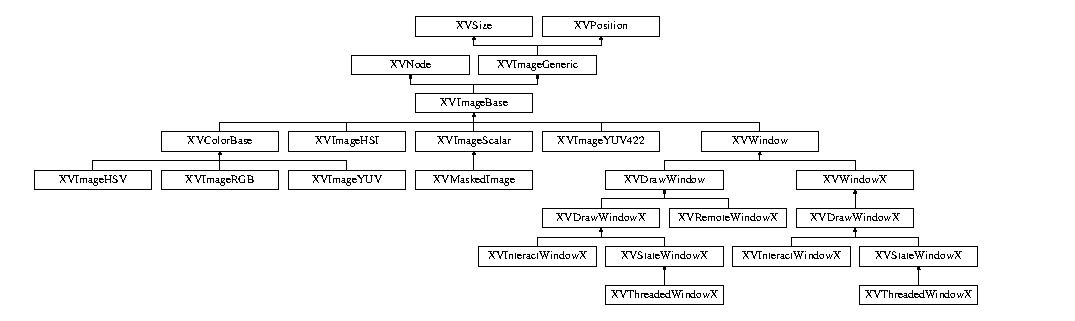
\includegraphics[height=3.86207cm]{class_XVImageBase}
\end{center}
\end{figure}
\subsection*{Public Types}
\begin{CompactItemize}
\item 
typedef T {\bf PIXELTYPE}
\end{CompactItemize}
\subsection*{Public Methods}
\begin{CompactItemize}
\item 
int \hyperlink{class_XVImageBase_a0}{Size\-X} (void) const
\begin{CompactList}\small\item\em Returns the width of the pixmap.\item\end{CompactList}\item 
int \hyperlink{class_XVImageBase_a1}{Size\-Y} (void) const
\begin{CompactList}\small\item\em Returns the height of the pixmap.\item\end{CompactList}\item 
const T$\ast$ \hyperlink{class_XVImageBase_a2}{data} () const
\begin{CompactList}\small\item\em Const Pointer.\item\end{CompactList}\item 
const T$\ast$ \hyperlink{class_XVImageBase_a3}{pix\-Data} () const
\begin{CompactList}\small\item\em Const Pointer.\item\end{CompactList}\item 
int \hyperlink{class_XVImageBase_a4}{Skip} () const
\begin{CompactList}\small\item\em Integer.\item\end{CompactList}\item 
virtual XVImage\_\-Type \hyperlink{class_XVImageBase_a5}{Image\-Type} () const
\begin{CompactList}\small\item\em Returns the image data type.\item\end{CompactList}\item 
T$\ast$ \hyperlink{class_XVImageBase_a6}{lock} (void)
\begin{CompactList}\small\item\em Locks the pixmap for this image, until you call unlock.\item\end{CompactList}\item 
bool \hyperlink{class_XVImageBase_a7}{unlock} (void)
\begin{CompactList}\small\item\em Unlocks the pixmap, making it available to be locked.\item\end{CompactList}\item 
void \hyperlink{class_XVImageBase_a8}{reposition} (const XVPosition \& xvp)
\begin{CompactList}\small\item\em Sets the "window" that the image affects within the pixmap.\item\end{CompactList}\item 
void {\bf reposition} (const int px, const int py)
\item 
void \hyperlink{class_XVImageBase_a10}{remap} (T $\ast$ addr,bool own\_\-flag=true)
\begin{CompactList}\small\item\em Sets a new position for the image data.\item\end{CompactList}\item 
const T$\ast$ \hyperlink{class_XVImageBase_a11}{operator\mbox{[}$\,$\mbox{]}} (int r) const
\begin{CompactList}\small\item\em Returns a pointer to the beginning of row r in the image.\item\end{CompactList}\item 
virtual void \hyperlink{class_XVImageBase_a12}{resize} (const int set\_\-width, const int set\_\-height)
\begin{CompactList}\small\item\em Resizes the image based on new width and height for the image.\item\end{CompactList}\item 
virtual void \hyperlink{class_XVImageBase_a13}{resize} (const \hyperlink{class_XVSize}{XVSize} \& xsize)
\begin{CompactList}\small\item\em Resizes the image based on the \hyperlink{class_XVSize}{XVSize} class.\item\end{CompactList}\item 
virtual void \hyperlink{class_XVImageBase_a14}{set\-Sub\-Image} (const \hyperlink{class_XVSize}{XVSize} \&, const XVPosition \&)
\begin{CompactList}\small\item\em Sets the window based on the \hyperlink{class_XVSize}{XVSize} and XVPosition classes.\item\end{CompactList}\item 
\label{XVImageBase_a15}
\hypertarget{class_XVImageBase_a15}{
\index{setSubImage@{setSubImage}!XVImageBase@{XVImage\-Base}}\index{XVImageBase@{XVImageBase}!setSubImage@{set\-Sub\-Image}}
virtual void {\bf set\-Sub\-Image} (int, int, int, int)}

\item 
\label{XVImageBase_a16}
\hypertarget{class_XVImageBase_a16}{
\index{setSubImage@{setSubImage}!XVImageBase@{XVImage\-Base}}\index{XVImageBase@{XVImageBase}!setSubImage@{set\-Sub\-Image}}
virtual void {\bf set\-Sub\-Image} (const \hyperlink{class_XVImageGeneric}{XVImage\-Generic} \&)}

\item 
virtual void \hyperlink{class_XVImageBase_a17}{set\-To\-Pixmap} ()
\begin{CompactList}\small\item\em Sets the image back to the entire pixmap.\item\end{CompactList}\item 
\hyperlink{class_XVImageBase_a18}{XVImage\-Base} (const int, const int, XVPixmap$<$T$>$ $\ast$ \hyperlink{class_XVImageBase_n1}{pixmap} = NULL)
\begin{CompactList}\small\item\em Constructs based on user parameters.\item\end{CompactList}\item 
\hyperlink{class_XVImageBase_a19}{XVImage\-Base} (const \hyperlink{class_XVSize}{XVSize} \&, XVPixmap$<$T$>$ $\ast$ \hyperlink{class_XVImageBase_n1}{pixmap} = NULL)
\begin{CompactList}\small\item\em Constructs based on an \hyperlink{class_XVSize}{XVSize} class, other parameters as above.\item\end{CompactList}\item 
\hyperlink{class_XVImageBase_a20}{XVImage\-Base} (const \hyperlink{class_XVImageGeneric}{XVImage\-Generic} \&, XVPixmap$<$T$>$ $\ast$ \hyperlink{class_XVImageBase_n1}{pixmap} = NULL)
\begin{CompactList}\small\item\em Constucts an image based on the pixmap passed in and defined by the region of interest.\item\end{CompactList}\item 
\label{XVImageBase_a21}
\hypertarget{class_XVImageBase_a21}{
\index{XVImageBase@{XVImageBase}!XVImageBase@{XVImage\-Base}}\index{XVImageBase@{XVImageBase}!XVImageBase@{XVImage\-Base}}
\hyperlink{class_XVImageBase_a21}{XVImage\-Base} (const XVImage\-Base$<$T$>$ \&im)}

\begin{CompactList}\small\item\em Copy constructor.\item\end{CompactList}\item 
\hyperlink{class_XVImageBase_a22}{XVImage\-Base} (XVPixmap$<$T$>$ $\ast$ \hyperlink{class_XVImageBase_n1}{pixmap})
\begin{CompactList}\small\item\em Constructor to cover the passed pixmap.\item\end{CompactList}\item 
\label{XVImageBase_a23}
\hypertarget{class_XVImageBase_a23}{
\index{XVImageBase@{XVImageBase}!XVImageBase@{XVImage\-Base}}\index{XVImageBase@{XVImageBase}!XVImageBase@{XVImage\-Base}}
{\bf XVImage\-Base} ()}

\item 
\label{XVImageBase_a24}
\hypertarget{class_XVImageBase_a24}{
\index{~XVImageBase@{$\sim$XVImageBase}!XVImageBase@{XVImage\-Base}}\index{XVImageBase@{XVImageBase}!~XVImageBase@{$\sim$XVImage\-Base}}
{\bf $\sim$XVImage\-Base} ()}

\item 
XVImage\-Base$<$T$>$\& \hyperlink{class_XVImageBase_a25}{operator=} (const XVImage\-Base$<$T$>$ \& im)
\begin{CompactList}\small\item\em WARNING: Please Read the Detailed Description.\item\end{CompactList}\end{CompactItemize}
\subsection*{Protected Attributes}
\begin{CompactItemize}
\item 
T$\ast$ \hyperlink{class_XVImageBase_n0}{win\_\-addr}
\begin{CompactList}\small\item\em Pointer.\item\end{CompactList}\item 
XVPixmap$<$T$>$$\ast$ \hyperlink{class_XVImageBase_n1}{pixmap}
\begin{CompactList}\small\item\em The pixmap containing this image.\item\end{CompactList}\item 
int \hyperlink{class_XVImageBase_n2}{lineskip}
\begin{CompactList}\small\item\em The number of memory elements between each leftmost pixel of a given row.\item\end{CompactList}\item 
int \hyperlink{class_XVImageBase_n3}{write\_\-perm}
\begin{CompactList}\small\item\em Whether this image can modify the underlying pixmap.\item\end{CompactList}\end{CompactItemize}
\subsection*{Friends}
\begin{CompactItemize}
\item 
class {\bf XVImage\-Iterator$<$ T $>$}
\end{CompactItemize}


\subsection{Detailed Description}
\subsubsection*{template$<$class T$>$  template class XVImage\-Base}

Base templated class for images.

XVImage\-Base contains the basics of an image which is defined as a full  or partial part of a pixmap upon which various operations can be performed. Base contains the basic operations, such as equality, output,  and dimensioning.  A basic "subimage" is defined in \hyperlink{class_XVImageGeneric}{XVImage\-Generic}, but only XVImage\-Base is templated, thus making XVImage\-Base ideal as the base class when any actions on the image data must take place. \par
The locking mechanism requires that locks be released on a pixmap before it will allow another image/iterators set to lock. That being said, all write iterators lock on construction and unlock on destruction. All write iterators based on an image must be destroyed in order for all locks to release and the way opened for a new image to lock.\par
 Locking Functions:\par
 XVPixmap::lock\_\-pixmap().\par
 \hyperlink{class_XVImageBase_a6}{XVImage\-Base::lock}(), and all derived classes.\par
 XVImage\-YUV::uv\_\-lock().\par
 XVImage\-WIterator::XVImage\-WIterator().\par
 Unlocking Functions:\par
 XVPixmap::unlock\_\-pixmap().\par
 \hyperlink{class_XVImageBase_a7}{XVImage\-Base::unlock}(), and all derived classes.\par
 XVImage\-YUV::uv\_\-unlock().\par
 XVImage\-WIterator::$\sim$XVImage\-WIterator().\par
 Sanity Check Functions:\par
 XVPixmap::get\_\-num\_\-locks().\par
 



Definition at line 335 of file XVImage\-Base.h.

\subsection{Member Typedef Documentation}
\label{XVImageBase_s0}
\hypertarget{class_XVImageBase_s0}{
\index{XVImageBase@{XVImage\-Base}!PIXELTYPE@{PIXELTYPE}}
\index{PIXELTYPE@{PIXELTYPE}!XVImageBase@{XVImage\-Base}}
\subsubsection[PIXELTYPE]{\setlength{\rightskip}{0pt plus 5cm}template$<$classT$>$ typedef T XVImage\-Base$<$T$>$::PIXELTYPE}}




Definition at line 339 of file XVImage\-Base.h.

\subsection{Constructor \& Destructor Documentation}
\label{XVImageBase_a18}
\hypertarget{class_XVImageBase_a18}{
\index{XVImageBase@{XVImage\-Base}!XVImageBase@{XVImageBase}}
\index{XVImageBase@{XVImageBase}!XVImageBase@{XVImage\-Base}}
\subsubsection[XVImageBase]{\setlength{\rightskip}{0pt plus 5cm}template$<$classT$>$ XVImage\-Base$<$T$>$::XVImage\-Base$<$T$>$ (const {\em int}, const {\em int}, XVPixmap$<$ T $>$$\ast$ {\em pixmap} = NULL)}}


Constructs based on user parameters.

If pixmap is NULL, it creates a new one the same size as the image.

PARAMTERS:

int width - the width of the image int height - the height of the image XVPixmap$<$T$>$ $\ast$ pixmap - the pixmap to set the image to (defaults to NULL) \label{XVImageBase_a19}
\hypertarget{class_XVImageBase_a19}{
\index{XVImageBase@{XVImage\-Base}!XVImageBase@{XVImageBase}}
\index{XVImageBase@{XVImageBase}!XVImageBase@{XVImage\-Base}}
\subsubsection[XVImageBase]{\setlength{\rightskip}{0pt plus 5cm}template$<$classT$>$ XVImage\-Base$<$T$>$::XVImage\-Base$<$T$>$ (const \hyperlink{class_XVSize}{XVSize} \&, XVPixmap$<$ T $>$$\ast$ {\em pixmap} = NULL)}}


Constructs based on an \hyperlink{class_XVSize}{XVSize} class, other parameters as above.

PARAMETERS:

\hyperlink{class_XVSize}{XVSize} \& size - reference to size of the new image XVPixmap$<$T$>$ $\ast$ - pointer to the pixmap to set this image to \label{XVImageBase_a20}
\hypertarget{class_XVImageBase_a20}{
\index{XVImageBase@{XVImage\-Base}!XVImageBase@{XVImageBase}}
\index{XVImageBase@{XVImageBase}!XVImageBase@{XVImage\-Base}}
\subsubsection[XVImageBase]{\setlength{\rightskip}{0pt plus 5cm}template$<$classT$>$ XVImage\-Base$<$T$>$::XVImage\-Base$<$T$>$ (const \hyperlink{class_XVImageGeneric}{XVImage\-Generic} \&, XVPixmap$<$ T $>$$\ast$ {\em pixmap} = NULL)}}


Constucts an image based on the pixmap passed in and defined by the region of interest.

PARAMETERS:

\hyperlink{class_XVImageGeneric}{XVImage\-Generic} roi - the region of interest to set this image to XVPixmap$<$T$>$ $\ast$ pixmap - the pixmap to set this image to refer to \label{XVImageBase_a22}
\hypertarget{class_XVImageBase_a22}{
\index{XVImageBase@{XVImage\-Base}!XVImageBase@{XVImageBase}}
\index{XVImageBase@{XVImageBase}!XVImageBase@{XVImage\-Base}}
\subsubsection[XVImageBase]{\setlength{\rightskip}{0pt plus 5cm}template$<$classT$>$ XVImage\-Base$<$T$>$::XVImage\-Base$<$T$>$ (XVPixmap$<$ T $>$$\ast$ {\em pixmap})}}


Constructor to cover the passed pixmap.

The entire passed pixmap falls into the scope of the new image. 

\subsection{Member Function Documentation}
\label{XVImageBase_a0}
\hypertarget{class_XVImageBase_a0}{
\index{XVImageBase@{XVImage\-Base}!SizeX@{SizeX}}
\index{SizeX@{SizeX}!XVImageBase@{XVImage\-Base}}
\subsubsection[SizeX]{\setlength{\rightskip}{0pt plus 5cm}template$<$classT$>$ int XVImage\-Base$<$T$>$::Size\-X (void) const\hspace{0.3cm}{\tt  \mbox{[}inline\mbox{]}}}}


Returns the width of the pixmap.



Definition at line 372 of file XVImage\-Base.h.\label{XVImageBase_a1}
\hypertarget{class_XVImageBase_a1}{
\index{XVImageBase@{XVImage\-Base}!SizeY@{SizeY}}
\index{SizeY@{SizeY}!XVImageBase@{XVImage\-Base}}
\subsubsection[SizeY]{\setlength{\rightskip}{0pt plus 5cm}template$<$classT$>$ int XVImage\-Base$<$T$>$::Size\-Y (void) const\hspace{0.3cm}{\tt  \mbox{[}inline\mbox{]}}}}


Returns the height of the pixmap.



Definition at line 377 of file XVImage\-Base.h.\label{XVImageBase_a2}
\hypertarget{class_XVImageBase_a2}{
\index{XVImageBase@{XVImage\-Base}!data@{data}}
\index{data@{data}!XVImageBase@{XVImage\-Base}}
\subsubsection[data]{\setlength{\rightskip}{0pt plus 5cm}template$<$classT$>$ const T $\ast$ XVImage\-Base$<$T$>$::data () const\hspace{0.3cm}{\tt  \mbox{[}inline\mbox{]}}}}


Const Pointer.

Returns the beginning of the image in the pixmap (const). 

Definition at line 383 of file XVImage\-Base.h.\label{XVImageBase_a3}
\hypertarget{class_XVImageBase_a3}{
\index{XVImageBase@{XVImage\-Base}!pixData@{pixData}}
\index{pixData@{pixData}!XVImageBase@{XVImage\-Base}}
\subsubsection[pixData]{\setlength{\rightskip}{0pt plus 5cm}template$<$classT$>$ const T $\ast$ XVImage\-Base$<$T$>$::pix\-Data () const\hspace{0.3cm}{\tt  \mbox{[}inline\mbox{]}}}}


Const Pointer.

Returns the beginning of the underlying pixmap (const). 

Definition at line 389 of file XVImage\-Base.h.\label{XVImageBase_a4}
\hypertarget{class_XVImageBase_a4}{
\index{XVImageBase@{XVImage\-Base}!Skip@{Skip}}
\index{Skip@{Skip}!XVImageBase@{XVImage\-Base}}
\subsubsection[Skip]{\setlength{\rightskip}{0pt plus 5cm}template$<$classT$>$ int XVImage\-Base$<$T$>$::Skip () const\hspace{0.3cm}{\tt  \mbox{[}inline\mbox{]}}}}


Integer.

Returns the lineskip value. 

Definition at line 395 of file XVImage\-Base.h.\label{XVImageBase_a5}
\hypertarget{class_XVImageBase_a5}{
\index{XVImageBase@{XVImage\-Base}!ImageType@{ImageType}}
\index{ImageType@{ImageType}!XVImageBase@{XVImage\-Base}}
\subsubsection[ImageType]{\setlength{\rightskip}{0pt plus 5cm}template$<$classT$>$ XVImage\_\-Type XVImage\-Base$<$T$>$::Image\-Type () const\hspace{0.3cm}{\tt  \mbox{[}inline, virtual\mbox{]}}}}


Returns the image data type.

Returns an XVImage\_\-Type (i.e. is XV\_\-RGB16). See XVImage\_\-Type. 

Definition at line 402 of file XVImage\-Base.h.\label{XVImageBase_a6}
\hypertarget{class_XVImageBase_a6}{
\index{XVImageBase@{XVImage\-Base}!lock@{lock}}
\index{lock@{lock}!XVImageBase@{XVImage\-Base}}
\subsubsection[lock]{\setlength{\rightskip}{0pt plus 5cm}template$<$classT$>$ T $\ast$ XVImage\-Base$<$T$>$::lock (void)\hspace{0.3cm}{\tt  \mbox{[}inline\mbox{]}}}}


Locks the pixmap for this image, until you call unlock.

Returns a pointer to the beginning of the image space in the pixmap if it successfully locks, otherwise returns NULL. See the general XVImage\-Base documentation for a description of the locking mechanism. 

Definition at line 411 of file XVImage\-Base.h.\label{XVImageBase_a7}
\hypertarget{class_XVImageBase_a7}{
\index{XVImageBase@{XVImage\-Base}!unlock@{unlock}}
\index{unlock@{unlock}!XVImageBase@{XVImage\-Base}}
\subsubsection[unlock]{\setlength{\rightskip}{0pt plus 5cm}template$<$classT$>$ bool XVImage\-Base$<$T$>$::unlock (void)\hspace{0.3cm}{\tt  \mbox{[}inline\mbox{]}}}}


Unlocks the pixmap, making it available to be locked.



Definition at line 419 of file XVImage\-Base.h.\label{XVImageBase_a8}
\hypertarget{class_XVImageBase_a8}{
\index{XVImageBase@{XVImage\-Base}!reposition@{reposition}}
\index{reposition@{reposition}!XVImageBase@{XVImage\-Base}}
\subsubsection[reposition]{\setlength{\rightskip}{0pt plus 5cm}template$<$classT$>$ void XVImage\-Base$<$T$>$::reposition (const XVPosition \& {\em xvp})\hspace{0.3cm}{\tt  \mbox{[}inline\mbox{]}}}}


Sets the "window" that the image affects within the pixmap.

Takes integer parameters. 

Definition at line 430 of file XVImage\-Base.h.\label{XVImageBase_a9}
\hypertarget{class_XVImageBase_a9}{
\index{XVImageBase@{XVImage\-Base}!reposition@{reposition}}
\index{reposition@{reposition}!XVImageBase@{XVImage\-Base}}
\subsubsection[reposition]{\setlength{\rightskip}{0pt plus 5cm}template$<$classT$>$ void XVImage\-Base$<$T$>$::reposition (const int {\em px}, const int {\em py})\hspace{0.3cm}{\tt  \mbox{[}inline\mbox{]}}}}




Definition at line 436 of file XVImage\-Base.h.\label{XVImageBase_a10}
\hypertarget{class_XVImageBase_a10}{
\index{XVImageBase@{XVImage\-Base}!remap@{remap}}
\index{remap@{remap}!XVImageBase@{XVImage\-Base}}
\subsubsection[remap]{\setlength{\rightskip}{0pt plus 5cm}template$<$classT$>$ void XVImage\-Base$<$T$>$::remap (T $\ast$ {\em addr}, bool {\em own\_\-flag} = true)}}


Sets a new position for the image data.

Used primarily for grabbing a frame from a framebuffer. \label{XVImageBase_a11}
\hypertarget{class_XVImageBase_a11}{
\index{XVImageBase@{XVImage\-Base}!operator[]@{operator[]}}
\index{operator[]@{operator[]}!XVImageBase@{XVImage\-Base}}
\subsubsection[operator{}]{\setlength{\rightskip}{0pt plus 5cm}template$<$classT$>$ const T $\ast$ XVImage\-Base$<$T$>$::operator\mbox{[}$\,$\mbox{]} (int {\em r}) const\hspace{0.3cm}{\tt  \mbox{[}inline\mbox{]}}}}


Returns a pointer to the beginning of row r in the image.



Definition at line 451 of file XVImage\-Base.h.\label{XVImageBase_a12}
\hypertarget{class_XVImageBase_a12}{
\index{XVImageBase@{XVImage\-Base}!resize@{resize}}
\index{resize@{resize}!XVImageBase@{XVImage\-Base}}
\subsubsection[resize]{\setlength{\rightskip}{0pt plus 5cm}template$<$classT$>$ void XVImage\-Base$<$T$>$::resize (const int {\em w}, const int {\em h})\hspace{0.3cm}{\tt  \mbox{[}virtual\mbox{]}}}}


Resizes the image based on new width and height for the image.

Takes integer parameters. 

Reimplemented from \hyperlink{class_XVSize_a9}{XVSize}.

Reimplemented in \hyperlink{class_XVWindowX_a3}{XVWindow\-X}.\label{XVImageBase_a13}
\hypertarget{class_XVImageBase_a13}{
\index{XVImageBase@{XVImage\-Base}!resize@{resize}}
\index{resize@{resize}!XVImageBase@{XVImage\-Base}}
\subsubsection[resize]{\setlength{\rightskip}{0pt plus 5cm}template$<$classT$>$ void XVImage\-Base$<$T$>$::resize (const \hyperlink{class_XVSize}{XVSize} \& {\em size})\hspace{0.3cm}{\tt  \mbox{[}virtual\mbox{]}}}}


Resizes the image based on the \hyperlink{class_XVSize}{XVSize} class.

For more information, see \hyperlink{class_XVSize}{XVSize}. 

Reimplemented from \hyperlink{class_XVSize_a8}{XVSize}.

Reimplemented in \hyperlink{class_XVRemoteWindowX_a9}{XVRemote\-Window\-X}, \hyperlink{class_XVWindow_a4}{XVWindow}, and \hyperlink{class_XVWindowX_a2}{XVWindow\-X}.\label{XVImageBase_a14}
\hypertarget{class_XVImageBase_a14}{
\index{XVImageBase@{XVImage\-Base}!setSubImage@{setSubImage}}
\index{setSubImage@{setSubImage}!XVImageBase@{XVImage\-Base}}
\subsubsection[setSubImage]{\setlength{\rightskip}{0pt plus 5cm}template$<$classT$>$ void XVImage\-Base$<$T$>$::set\-Sub\-Image (const \hyperlink{class_XVSize}{XVSize} \&, const XVPosition \&)\hspace{0.3cm}{\tt  \mbox{[}virtual\mbox{]}}}}


Sets the window based on the \hyperlink{class_XVSize}{XVSize} and XVPosition classes.

For more information see \hyperlink{class_XVSize}{XVSize} and XVPosition. 

Referenced by set\-To\-Pixmap().\label{XVImageBase_a17}
\hypertarget{class_XVImageBase_a17}{
\index{XVImageBase@{XVImage\-Base}!setToPixmap@{setToPixmap}}
\index{setToPixmap@{setToPixmap}!XVImageBase@{XVImage\-Base}}
\subsubsection[setToPixmap]{\setlength{\rightskip}{0pt plus 5cm}template$<$classT$>$ void XVImage\-Base$<$T$>$::set\-To\-Pixmap ()\hspace{0.3cm}{\tt  \mbox{[}inline, virtual\mbox{]}}}}


Sets the image back to the entire pixmap.



Definition at line 477 of file XVImage\-Base.h.\label{XVImageBase_a25}
\hypertarget{class_XVImageBase_a25}{
\index{XVImageBase@{XVImage\-Base}!operator=@{operator=}}
\index{operator=@{operator=}!XVImageBase@{XVImage\-Base}}
\subsubsection[operator=]{\setlength{\rightskip}{0pt plus 5cm}template$<$classT$>$ XVImage\-Base$<$ T $>$\& XVImage\-Base$<$T$>$::operator= (const XVImage\-Base$<$ T $>$\& {\em im})}}


WARNING: Please Read the Detailed Description.

If SLOW\_\-COPY is defined (not default), the method of assignment is a pixel by pixel copy. While very safe, this takes time, and is accordingly a slow copy. If SLOW\_\-COPY is not defined (default) the method of assignment is via "pointer-swinging": the pointer to  Image A's pixmap is assigned and registered as the pixmap pointer  for Image B, and the Image parameters (height, width, position, etc.) are then copied. While much faster than the SLOW\_\-COPY method, this may may not be what you are expecting. After assignment, both images A and B will modify the same data! 

\subsection{Friends And Related Function Documentation}
\label{XVImageBase_l0}
\hypertarget{class_XVImageBase_l0}{
\index{XVImageBase@{XVImage\-Base}!XVImageIterator< T >@{XVImageIterator$<$ T $>$}}
\index{XVImageIterator< T >@{XVImageIterator$<$ T $>$}!XVImageBase@{XVImage\-Base}}
\subsubsection[XVImageIterator< T >]{\setlength{\rightskip}{0pt plus 5cm}template$<$classT$>$ class XVImage\-Iterator\hspace{0.3cm}{\tt  \mbox{[}friend\mbox{]}}}}




Definition at line 341 of file XVImage\-Base.h.

\subsection{Member Data Documentation}
\label{XVImageBase_n0}
\hypertarget{class_XVImageBase_n0}{
\index{XVImageBase@{XVImage\-Base}!win_addr@{win\_\-addr}}
\index{win_addr@{win\_\-addr}!XVImageBase@{XVImage\-Base}}
\subsubsection[win_addr]{\setlength{\rightskip}{0pt plus 5cm}template$<$classT$>$ T $\ast$ XVImage\-Base$<$T$>$::win\_\-addr\hspace{0.3cm}{\tt  \mbox{[}protected\mbox{]}}}}


Pointer.

The address of the image in the pixmap. 

Definition at line 348 of file XVImage\-Base.h.\label{XVImageBase_n1}
\hypertarget{class_XVImageBase_n1}{
\index{XVImageBase@{XVImage\-Base}!pixmap@{pixmap}}
\index{pixmap@{pixmap}!XVImageBase@{XVImage\-Base}}
\subsubsection[pixmap]{\setlength{\rightskip}{0pt plus 5cm}template$<$classT$>$ XVPixmap$<$ T $>$$\ast$ XVImage\-Base$<$T$>$::pixmap\hspace{0.3cm}{\tt  \mbox{[}protected\mbox{]}}}}


The pixmap containing this image.



Definition at line 353 of file XVImage\-Base.h.\label{XVImageBase_n2}
\hypertarget{class_XVImageBase_n2}{
\index{XVImageBase@{XVImage\-Base}!lineskip@{lineskip}}
\index{lineskip@{lineskip}!XVImageBase@{XVImage\-Base}}
\subsubsection[lineskip]{\setlength{\rightskip}{0pt plus 5cm}template$<$classT$>$ int XVImage\-Base$<$T$>$::lineskip\hspace{0.3cm}{\tt  \mbox{[}protected\mbox{]}}}}


The number of memory elements between each leftmost pixel of a given row.



Definition at line 359 of file XVImage\-Base.h.\label{XVImageBase_n3}
\hypertarget{class_XVImageBase_n3}{
\index{XVImageBase@{XVImage\-Base}!write_perm@{write\_\-perm}}
\index{write_perm@{write\_\-perm}!XVImageBase@{XVImage\-Base}}
\subsubsection[write_perm]{\setlength{\rightskip}{0pt plus 5cm}template$<$classT$>$ int XVImage\-Base$<$T$>$::write\_\-perm\hspace{0.3cm}{\tt  \mbox{[}protected\mbox{]}}}}


Whether this image can modify the underlying pixmap.



Definition at line 365 of file XVImage\-Base.h.

The documentation for this class was generated from the following file:\begin{CompactItemize}
\item 
/home/burschka/XVision2-2.0.0/src/Images/\hyperlink{XVImageBase.h-source}{XVImage\-Base.h}\end{CompactItemize}

\hypertarget{class_XVImageException}{
\section{XVImage\-Exception  Class Reference}
\label{XVImageException}\index{XVImageException@{XVImage\-Exception}}
}
exception class for XVImages. 


{\tt \#include $<$XVImage\-Base.h$>$}

Inheritance diagram for XVImage\-Exception:\begin{figure}[H]
\begin{center}
\leavevmode
\includegraphics[height=3cm]{class_XVImageException}
\end{center}
\end{figure}
\subsection*{Public Methods}
\begin{CompactItemize}
\item 
{\bf XVImage\-Exception} ()
\item 
{\bf XVImage\-Exception} (char $\ast$ err)
\end{CompactItemize}


\subsection{Detailed Description}
exception class for XVImages.





Definition at line 20 of file XVImage\-Base.h.

\subsection{Constructor \& Destructor Documentation}
\label{XVImageException_a0}
\hypertarget{class_XVImageException_a0}{
\index{XVImageException@{XVImage\-Exception}!XVImageException@{XVImageException}}
\index{XVImageException@{XVImageException}!XVImageException@{XVImage\-Exception}}
\subsubsection[XVImageException]{\setlength{\rightskip}{0pt plus 5cm}XVImage\-Exception::XVImage\-Exception ()}}




Definition at line 21 of file XVImage\-Base.h.\label{XVImageException_a1}
\hypertarget{class_XVImageException_a1}{
\index{XVImageException@{XVImage\-Exception}!XVImageException@{XVImageException}}
\index{XVImageException@{XVImageException}!XVImageException@{XVImage\-Exception}}
\subsubsection[XVImageException]{\setlength{\rightskip}{0pt plus 5cm}XVImage\-Exception::XVImage\-Exception (char $\ast$ {\em err})}}




Definition at line 22 of file XVImage\-Base.h.

The documentation for this class was generated from the following file:\begin{CompactItemize}
\item 
/home/burschka/XVision2-2.0.0/src/Images/\hyperlink{XVImageBase.h-source}{XVImage\-Base.h}\end{CompactItemize}

\hypertarget{class_XVImageGeneric}{
\section{XVImage\-Generic  Class Reference}
\label{XVImageGeneric}\index{XVImageGeneric@{XVImage\-Generic}}
}
Very basic definition (non-templated) of an image. 


{\tt \#include $<$XVImage\-Base.h$>$}

Inheritance diagram for XVImage\-Generic:\begin{figure}[H]
\begin{center}
\leavevmode
\includegraphics[height=3.57013cm]{class_XVImageGeneric}
\end{center}
\end{figure}
\subsection*{Public Methods}
\begin{CompactItemize}
\item 
{\bf XVImage\-Generic} (const \hyperlink{class_XVSize}{XVSize} \&xsize, const XVPosition \&xvp)
\item 
{\bf XVImage\-Generic} (const \hyperlink{class_XVSize}{XVSize} \&xsize)
\item 
{\bf XVImage\-Generic} (const int cw, const int rh, const int px = 0, const int py = 0)
\item 
{\bf XVImage\-Generic} ()
\item 
{\bf XVImage\-Generic} (const XVImage\-Generic \&xvg)
\item 
bool \hyperlink{class_XVImageGeneric_a5}{within} (const XVImage\-Generic \& outer) const
\begin{CompactList}\small\item\em Checks if this region is completely bounded by another.\item\end{CompactList}\item 
bool \hyperlink{class_XVImageGeneric_a6}{contains} (const XVPosition \& pos) const
\begin{CompactList}\small\item\em checks if a point is contained by this region.\item\end{CompactList}\end{CompactItemize}


\subsection{Detailed Description}
Very basic definition (non-templated) of an image.

XVImage\-Generic specifies the dimension aspects of a image, but due to its a lack of templatization, it is suitable as  the definition of a "window." If you need to use the data from image, use \hyperlink{class_XVImageBase}{XVImage\-Base}. 



Definition at line 241 of file XVImage\-Base.h.

\subsection{Constructor \& Destructor Documentation}
\label{XVImageGeneric_a0}
\hypertarget{class_XVImageGeneric_a0}{
\index{XVImageGeneric@{XVImage\-Generic}!XVImageGeneric@{XVImageGeneric}}
\index{XVImageGeneric@{XVImageGeneric}!XVImageGeneric@{XVImage\-Generic}}
\subsubsection[XVImageGeneric]{\setlength{\rightskip}{0pt plus 5cm}XVImage\-Generic::XVImage\-Generic (const \hyperlink{class_XVSize}{XVSize} \& {\em xsize}, const XVPosition \& {\em xvp})}}




Definition at line 245 of file XVImage\-Base.h.\label{XVImageGeneric_a1}
\hypertarget{class_XVImageGeneric_a1}{
\index{XVImageGeneric@{XVImage\-Generic}!XVImageGeneric@{XVImageGeneric}}
\index{XVImageGeneric@{XVImageGeneric}!XVImageGeneric@{XVImage\-Generic}}
\subsubsection[XVImageGeneric]{\setlength{\rightskip}{0pt plus 5cm}XVImage\-Generic::XVImage\-Generic (const \hyperlink{class_XVSize}{XVSize} \& {\em xsize})}}




Definition at line 248 of file XVImage\-Base.h.\label{XVImageGeneric_a2}
\hypertarget{class_XVImageGeneric_a2}{
\index{XVImageGeneric@{XVImage\-Generic}!XVImageGeneric@{XVImageGeneric}}
\index{XVImageGeneric@{XVImageGeneric}!XVImageGeneric@{XVImage\-Generic}}
\subsubsection[XVImageGeneric]{\setlength{\rightskip}{0pt plus 5cm}XVImage\-Generic::XVImage\-Generic (const int {\em cw}, const int {\em rh}, const int {\em px} = 0, const int {\em py} = 0)}}




Definition at line 251 of file XVImage\-Base.h.\label{XVImageGeneric_a3}
\hypertarget{class_XVImageGeneric_a3}{
\index{XVImageGeneric@{XVImage\-Generic}!XVImageGeneric@{XVImageGeneric}}
\index{XVImageGeneric@{XVImageGeneric}!XVImageGeneric@{XVImage\-Generic}}
\subsubsection[XVImageGeneric]{\setlength{\rightskip}{0pt plus 5cm}XVImage\-Generic::XVImage\-Generic ()}}




Definition at line 254 of file XVImage\-Base.h.\label{XVImageGeneric_a4}
\hypertarget{class_XVImageGeneric_a4}{
\index{XVImageGeneric@{XVImage\-Generic}!XVImageGeneric@{XVImageGeneric}}
\index{XVImageGeneric@{XVImageGeneric}!XVImageGeneric@{XVImage\-Generic}}
\subsubsection[XVImageGeneric]{\setlength{\rightskip}{0pt plus 5cm}XVImage\-Generic::XVImage\-Generic (const XVImage\-Generic \& {\em xvg})}}




Definition at line 256 of file XVImage\-Base.h.

\subsection{Member Function Documentation}
\label{XVImageGeneric_a5}
\hypertarget{class_XVImageGeneric_a5}{
\index{XVImageGeneric@{XVImage\-Generic}!within@{within}}
\index{within@{within}!XVImageGeneric@{XVImage\-Generic}}
\subsubsection[within]{\setlength{\rightskip}{0pt plus 5cm}bool XVImage\-Generic::within (const XVImage\-Generic \& {\em outer}) const\hspace{0.3cm}{\tt  \mbox{[}inline\mbox{]}}}}


Checks if this region is completely bounded by another.

This region is within the outer region if this region's boundary is within or on the boundary of the outer region. 

Definition at line 264 of file XVImage\-Base.h.\label{XVImageGeneric_a6}
\hypertarget{class_XVImageGeneric_a6}{
\index{XVImageGeneric@{XVImage\-Generic}!contains@{contains}}
\index{contains@{contains}!XVImageGeneric@{XVImage\-Generic}}
\subsubsection[contains]{\setlength{\rightskip}{0pt plus 5cm}bool XVImage\-Generic::contains (const XVPosition \& {\em pos}) const\hspace{0.3cm}{\tt  \mbox{[}inline\mbox{]}}}}


checks if a point is contained by this region.

The point is contained by the region if the  the point is inside or on the boundary of the  region. 

Definition at line 276 of file XVImage\-Base.h.

The documentation for this class was generated from the following file:\begin{CompactItemize}
\item 
/home/burschka/XVision2-2.0.0/src/Images/\hyperlink{XVImageBase.h-source}{XVImage\-Base.h}\end{CompactItemize}

\hypertarget{class_XVImageHSI}{
\section{XVImage\-HSI  Template Class Reference}
\label{XVImageHSI}\index{XVImageHSI@{XVImage\-HSI}}
}
class for HSI images. 


{\tt \#include $<$XVImage\-HSI.h$>$}

Inheritance diagram for XVImage\-HSI:\begin{figure}[H]
\begin{center}
\leavevmode
\includegraphics[height=4cm]{class_XVImageHSI}
\end{center}
\end{figure}
\subsection*{Public Methods}
\begin{CompactItemize}
\item 
{\bf XVImage\-HSI} (int width, int height, XVPixmap$<$T$>$ $\ast$\hyperlink{class_XVImageBase_n1}{pixmap}=NULL, char $\ast$title=NULL)
\item 
{\bf XVImage\-HSI} (XVPixmap$<$T$>$ $\ast$\hyperlink{class_XVImageBase_n1}{pixmap})
\item 
{\bf XVImage\-HSI} ()
\end{CompactItemize}


\subsection{Detailed Description}
\subsubsection*{template$<$class T$>$  template class XVImage\-HSI}

class for HSI images.





Definition at line 16 of file XVImage\-HSI.h.

\subsection{Constructor \& Destructor Documentation}
\label{XVImageHSI_a0}
\hypertarget{class_XVImageHSI_a0}{
\index{XVImageHSI@{XVImage\-HSI}!XVImageHSI@{XVImageHSI}}
\index{XVImageHSI@{XVImageHSI}!XVImageHSI@{XVImage\-HSI}}
\subsubsection[XVImageHSI]{\setlength{\rightskip}{0pt plus 5cm}template$<$classT$>$ XVImage\-HSI$<$T$>$::XVImage\-HSI$<$T$>$ (int {\em width}, int {\em height}, XVPixmap$<$ T $>$$\ast$ {\em pixmap} = NULL, char $\ast$ {\em title} = NULL)}}




Definition at line 19 of file XVImage\-HSI.h.\label{XVImageHSI_a1}
\hypertarget{class_XVImageHSI_a1}{
\index{XVImageHSI@{XVImage\-HSI}!XVImageHSI@{XVImageHSI}}
\index{XVImageHSI@{XVImageHSI}!XVImageHSI@{XVImage\-HSI}}
\subsubsection[XVImageHSI]{\setlength{\rightskip}{0pt plus 5cm}template$<$classT$>$ XVImage\-HSI$<$T$>$::XVImage\-HSI$<$T$>$ (XVPixmap$<$ T $>$$\ast$ {\em pixmap})}}




Definition at line 21 of file XVImage\-HSI.h.\label{XVImageHSI_a2}
\hypertarget{class_XVImageHSI_a2}{
\index{XVImageHSI@{XVImage\-HSI}!XVImageHSI@{XVImageHSI}}
\index{XVImageHSI@{XVImageHSI}!XVImageHSI@{XVImage\-HSI}}
\subsubsection[XVImageHSI]{\setlength{\rightskip}{0pt plus 5cm}template$<$classT$>$ XVImage\-HSI$<$T$>$::XVImage\-HSI$<$T$>$ ()}}




Definition at line 22 of file XVImage\-HSI.h.

The documentation for this class was generated from the following file:\begin{CompactItemize}
\item 
/home/burschka/XVision2-2.0.0/src/Images/\hyperlink{XVImageHSI.h-source}{XVImage\-HSI.h}\end{CompactItemize}

\hypertarget{class_XVImageHSV}{
\section{XVImage\-HSV  Template Class Reference}
\label{XVImageHSV}\index{XVImageHSV@{XVImage\-HSV}}
}
class for HSV images. 


{\tt \#include $<$XVImage\-HSV.h$>$}

Inheritance diagram for XVImage\-HSV:\begin{figure}[H]
\begin{center}
\leavevmode
\includegraphics[height=5cm]{class_XVImageHSV}
\end{center}
\end{figure}
\subsection*{Public Methods}
\begin{CompactItemize}
\item 
{\bf XVImage\-HSV} (int width, int height, XVPixmap$<$T$>$ $\ast$ \hyperlink{class_XVImageBase_n1}{pixmap} = NULL)
\item 
{\bf XVImage\-HSV} (\hyperlink{class_XVSize}{XVSize} s, XVPixmap$<$T$>$ $\ast$ p )
\item 
{\bf XVImage\-HSV} (XVPixmap$<$T$>$ $\ast$ \hyperlink{class_XVImageBase_n1}{pixmap})
\item 
{\bf XVImage\-HSV} ()
\end{CompactItemize}


\subsection{Detailed Description}
\subsubsection*{template$<$class T$>$  template class XVImage\-HSV}

class for HSV images.





Definition at line 21 of file XVImage\-HSV.h.

\subsection{Constructor \& Destructor Documentation}
\label{XVImageHSV_a0}
\hypertarget{class_XVImageHSV_a0}{
\index{XVImageHSV@{XVImage\-HSV}!XVImageHSV@{XVImageHSV}}
\index{XVImageHSV@{XVImageHSV}!XVImageHSV@{XVImage\-HSV}}
\subsubsection[XVImageHSV]{\setlength{\rightskip}{0pt plus 5cm}template$<$classT$>$ XVImage\-HSV$<$T$>$::XVImage\-HSV$<$T$>$ (int {\em width}, int {\em height}, XVPixmap$<$ T $>$$\ast$ {\em pixmap} = NULL)}}




Definition at line 25 of file XVImage\-HSV.h.\label{XVImageHSV_a1}
\hypertarget{class_XVImageHSV_a1}{
\index{XVImageHSV@{XVImage\-HSV}!XVImageHSV@{XVImageHSV}}
\index{XVImageHSV@{XVImageHSV}!XVImageHSV@{XVImage\-HSV}}
\subsubsection[XVImageHSV]{\setlength{\rightskip}{0pt plus 5cm}template$<$classT$>$ XVImage\-HSV$<$T$>$::XVImage\-HSV$<$T$>$ (\hyperlink{class_XVSize}{XVSize} {\em s}, XVPixmap$<$ T $>$$\ast$ {\em p})}}




Definition at line 27 of file XVImage\-HSV.h.\label{XVImageHSV_a2}
\hypertarget{class_XVImageHSV_a2}{
\index{XVImageHSV@{XVImage\-HSV}!XVImageHSV@{XVImageHSV}}
\index{XVImageHSV@{XVImageHSV}!XVImageHSV@{XVImage\-HSV}}
\subsubsection[XVImageHSV]{\setlength{\rightskip}{0pt plus 5cm}template$<$classT$>$ XVImage\-HSV$<$T$>$::XVImage\-HSV$<$T$>$ (XVPixmap$<$ T $>$$\ast$ {\em pixmap})}}




Definition at line 30 of file XVImage\-HSV.h.\label{XVImageHSV_a3}
\hypertarget{class_XVImageHSV_a3}{
\index{XVImageHSV@{XVImage\-HSV}!XVImageHSV@{XVImageHSV}}
\index{XVImageHSV@{XVImageHSV}!XVImageHSV@{XVImage\-HSV}}
\subsubsection[XVImageHSV]{\setlength{\rightskip}{0pt plus 5cm}template$<$classT$>$ XVImage\-HSV$<$T$>$::XVImage\-HSV$<$T$>$ ()}}




Definition at line 31 of file XVImage\-HSV.h.

The documentation for this class was generated from the following file:\begin{CompactItemize}
\item 
/home/burschka/XVision2-2.0.0/src/Images/\hyperlink{XVImageHSV.h-source}{XVImage\-HSV.h}\end{CompactItemize}

\hypertarget{class_XVImageRGB}{
\section{XVImage\-RGB  Template Class Reference}
\label{XVImageRGB}\index{XVImageRGB@{XVImage\-RGB}}
}
class for RGB images. 


{\tt \#include $<$XVImage\-RGB.h$>$}

Inheritance diagram for XVImage\-RGB:\begin{figure}[H]
\begin{center}
\leavevmode
\includegraphics[height=5cm]{class_XVImageRGB}
\end{center}
\end{figure}
\subsection*{Public Methods}
\begin{CompactItemize}
\item 
{\bf XVImage\-RGB} (int width, int height, XVPixmap$<$T$>$ $\ast$ \hyperlink{class_XVImageBase_n1}{pixmap} = NULL)
\item 
{\bf XVImage\-RGB} (\hyperlink{class_XVSize}{XVSize} s, XVPixmap$<$T$>$ $\ast$ p )
\item 
{\bf XVImage\-RGB} (XVPixmap$<$T$>$ $\ast$ \hyperlink{class_XVImageBase_n1}{pixmap})
\item 
{\bf XVImage\-RGB} ()
\end{CompactItemize}


\subsection{Detailed Description}
\subsubsection*{template$<$class T$>$  template class XVImage\-RGB}

class for RGB images.





Definition at line 18 of file XVImage\-RGB.h.

\subsection{Constructor \& Destructor Documentation}
\label{XVImageRGB_a0}
\hypertarget{class_XVImageRGB_a0}{
\index{XVImageRGB@{XVImage\-RGB}!XVImageRGB@{XVImageRGB}}
\index{XVImageRGB@{XVImageRGB}!XVImageRGB@{XVImage\-RGB}}
\subsubsection[XVImageRGB]{\setlength{\rightskip}{0pt plus 5cm}template$<$classT$>$ XVImage\-RGB$<$T$>$::XVImage\-RGB$<$T$>$ (int {\em width}, int {\em height}, XVPixmap$<$ T $>$$\ast$ {\em pixmap} = NULL)}}




Definition at line 22 of file XVImage\-RGB.h.\label{XVImageRGB_a1}
\hypertarget{class_XVImageRGB_a1}{
\index{XVImageRGB@{XVImage\-RGB}!XVImageRGB@{XVImageRGB}}
\index{XVImageRGB@{XVImageRGB}!XVImageRGB@{XVImage\-RGB}}
\subsubsection[XVImageRGB]{\setlength{\rightskip}{0pt plus 5cm}template$<$classT$>$ XVImage\-RGB$<$T$>$::XVImage\-RGB$<$T$>$ (\hyperlink{class_XVSize}{XVSize} {\em s}, XVPixmap$<$ T $>$$\ast$ {\em p})}}




Definition at line 24 of file XVImage\-RGB.h.\label{XVImageRGB_a2}
\hypertarget{class_XVImageRGB_a2}{
\index{XVImageRGB@{XVImage\-RGB}!XVImageRGB@{XVImageRGB}}
\index{XVImageRGB@{XVImageRGB}!XVImageRGB@{XVImage\-RGB}}
\subsubsection[XVImageRGB]{\setlength{\rightskip}{0pt plus 5cm}template$<$classT$>$ XVImage\-RGB$<$T$>$::XVImage\-RGB$<$T$>$ (XVPixmap$<$ T $>$$\ast$ {\em pixmap})}}




Definition at line 27 of file XVImage\-RGB.h.\label{XVImageRGB_a3}
\hypertarget{class_XVImageRGB_a3}{
\index{XVImageRGB@{XVImage\-RGB}!XVImageRGB@{XVImageRGB}}
\index{XVImageRGB@{XVImageRGB}!XVImageRGB@{XVImage\-RGB}}
\subsubsection[XVImageRGB]{\setlength{\rightskip}{0pt plus 5cm}template$<$classT$>$ XVImage\-RGB$<$T$>$::XVImage\-RGB$<$T$>$ ()}}




Definition at line 28 of file XVImage\-RGB.h.

The documentation for this class was generated from the following file:\begin{CompactItemize}
\item 
/home/burschka/XVision2-2.0.0/src/Images/\hyperlink{XVImageRGB.h-source}{XVImage\-RGB.h}\end{CompactItemize}

\hypertarget{class_XVImageScalar}{
\section{XVImage\-Scalar  Template Class Reference}
\label{XVImageScalar}\index{XVImageScalar@{XVImage\-Scalar}}
}
Defines an image with scalar operations. 


{\tt \#include $<$XVImage\-Scalar.h$>$}

Inheritance diagram for XVImage\-Scalar:\begin{figure}[H]
\begin{center}
\leavevmode
\includegraphics[height=5cm]{class_XVImageScalar}
\end{center}
\end{figure}
\subsection*{Public Methods}
\begin{CompactItemize}
\item 
{\bf XVImage\-Scalar} (int width, int height, XVPixmap$<$T$>$ $\ast$ \hyperlink{class_XVImageBase_n1}{pixmap} = NULL)
\item 
{\bf XVImage\-Scalar} (const \hyperlink{class_XVSize}{XVSize} \& s, XVPixmap$<$T$>$ $\ast$ p )
\item 
{\bf XVImage\-Scalar} (XVPixmap$<$T$>$ $\ast$ \hyperlink{class_XVImageBase_n1}{pixmap})
\item 
{\bf XVImage\-Scalar} ()
\item 
\label{XVImageScalar_a4}
\hypertarget{class_XVImageScalar_a4}{
\index{operator XVImageRGB@{operator XVImageRGB}!XVImageScalar@{XVImage\-Scalar}}\index{XVImageScalar@{XVImageScalar}!operator XVImageRGB@{operator XVImage\-RGB}}
{\bf operator XVImage\-RGB} () const}

\item 
\label{XVImageScalar_a5}
\hypertarget{class_XVImageScalar_a5}{
\index{operator XVImageRGB@{operator XVImageRGB}!XVImageScalar@{XVImage\-Scalar}}\index{XVImageScalar@{XVImageScalar}!operator XVImageRGB@{operator XVImage\-RGB}}
{\bf operator XVImage\-RGB} () const}

\item 
\label{XVImageScalar_a6}
\hypertarget{class_XVImageScalar_a6}{
\index{operator XVImageRGB@{operator XVImageRGB}!XVImageScalar@{XVImage\-Scalar}}\index{XVImageScalar@{XVImageScalar}!operator XVImageRGB@{operator XVImage\-RGB}}
{\bf operator XVImage\-RGB} () const}

\item 
\label{XVImageScalar_a7}
\hypertarget{class_XVImageScalar_a7}{
\index{operator XVImageRGB@{operator XVImageRGB}!XVImageScalar@{XVImage\-Scalar}}\index{XVImageScalar@{XVImageScalar}!operator XVImageRGB@{operator XVImage\-RGB}}
{\bf operator XVImage\-RGB} () const}

\item 
\label{XVImageScalar_a8}
\hypertarget{class_XVImageScalar_a8}{
\index{operator XVImageRGB@{operator XVImageRGB}!XVImageScalar@{XVImage\-Scalar}}\index{XVImageScalar@{XVImageScalar}!operator XVImageRGB@{operator XVImage\-RGB}}
{\bf operator XVImage\-RGB} () const}

\item 
\label{XVImageScalar_a9}
\hypertarget{class_XVImageScalar_a9}{
\index{operator XVImageRGB@{operator XVImageRGB}!XVImageScalar@{XVImage\-Scalar}}\index{XVImageScalar@{XVImageScalar}!operator XVImageRGB@{operator XVImage\-RGB}}
{\bf operator XVImage\-RGB} () const}

\item 
\label{XVImageScalar_a10}
\hypertarget{class_XVImageScalar_a10}{
\index{operator XVImageYUV@{operator XVImageYUV}!XVImageScalar@{XVImage\-Scalar}}\index{XVImageScalar@{XVImageScalar}!operator XVImageYUV@{operator XVImage\-YUV}}
{\bf operator XVImage\-YUV} () const}

\item 
\label{XVImageScalar_a11}
\hypertarget{class_XVImageScalar_a11}{
\index{operator XVImageHSV@{operator XVImageHSV}!XVImageScalar@{XVImage\-Scalar}}\index{XVImageScalar@{XVImageScalar}!operator XVImageHSV@{operator XVImage\-HSV}}
{\bf operator XVImage\-HSV} () const}

\item 
\label{XVImageScalar_a12}
\hypertarget{class_XVImageScalar_a12}{
\index{operator XVImageYUV422@{operator XVImageYUV422}!XVImageScalar@{XVImage\-Scalar}}\index{XVImageScalar@{XVImageScalar}!operator XVImageYUV422@{operator XVImage\-YUV422}}
{\bf operator XVImage\-YUV422} () const}

\item 
template$<$classT2$>$ {\bf operator XVImage\-Scalar}$<$T2$>$ () const
\item 
\label{XVImageScalar_a14}
\hypertarget{class_XVImageScalar_a14}{
\index{mean@{mean}!XVImageScalar@{XVImage\-Scalar}}\index{XVImageScalar@{XVImageScalar}!mean@{mean}}
T {\bf mean} () const}

\item 
\label{XVImageScalar_a15}
\hypertarget{class_XVImageScalar_a15}{
\index{avg@{avg}!XVImageScalar@{XVImage\-Scalar}}\index{XVImageScalar@{XVImageScalar}!avg@{avg}}
T {\bf avg} () const}

\item 
\label{XVImageScalar_a16}
\hypertarget{class_XVImageScalar_a16}{
\index{sum@{sum}!XVImageScalar@{XVImage\-Scalar}}\index{XVImageScalar@{XVImageScalar}!sum@{sum}}
T {\bf sum} () const}

\item 
\label{XVImageScalar_a17}
\hypertarget{class_XVImageScalar_a17}{
\index{operator+=@{operator+=}!XVImageScalar@{XVImage\-Scalar}}\index{XVImageScalar@{XVImageScalar}!operator+=@{operator+=}}
XVImage\-Scalar$<$T$>$\& \hyperlink{class_XVImageScalar_a17}{operator+=} (const XVImage\-Scalar$<$T$>$ \&)}

\begin{CompactList}\small\item\em Adds to each pixel in the image the corresponding pixel in the image passed in.\item\end{CompactList}\item 
\label{XVImageScalar_a18}
\hypertarget{class_XVImageScalar_a18}{
\index{operator-=@{operator-=}!XVImageScalar@{XVImage\-Scalar}}\index{XVImageScalar@{XVImageScalar}!operator-=@{operator-=}}
XVImage\-Scalar$<$T$>$\& \hyperlink{class_XVImageScalar_a18}{operator-=} (const XVImage\-Scalar$<$T$>$ \&)}

\begin{CompactList}\small\item\em Subtracts from each pixel in the image the corresponding pixel in the image passed in.\item\end{CompactList}\item 
\label{XVImageScalar_a19}
\hypertarget{class_XVImageScalar_a19}{
\index{operator *=@{operator $\ast$=}!XVImageScalar@{XVImage\-Scalar}}\index{XVImageScalar@{XVImageScalar}!operator *=@{operator $\ast$=}}
XVImage\-Scalar$<$T$>$\& \hyperlink{class_XVImageScalar_a19}{operator $\ast$=} (const XVImage\-Scalar$<$T$>$ \&)}

\begin{CompactList}\small\item\em Multiplies each pixel in the image by the corresponding pixel in the image passed in.\item\end{CompactList}\item 
\label{XVImageScalar_a20}
\hypertarget{class_XVImageScalar_a20}{
\index{operator/=@{operator/=}!XVImageScalar@{XVImage\-Scalar}}\index{XVImageScalar@{XVImageScalar}!operator/=@{operator/=}}
XVImage\-Scalar$<$T$>$\& \hyperlink{class_XVImageScalar_a20}{operator/=} (const XVImage\-Scalar$<$T$>$ \&)}

\begin{CompactList}\small\item\em Divides each pixel in the image by the corresponding pixel in the image passed in.\item\end{CompactList}\item 
\label{XVImageScalar_a21}
\hypertarget{class_XVImageScalar_a21}{
\index{operator=@{operator=}!XVImageScalar@{XVImage\-Scalar}}\index{XVImageScalar@{XVImageScalar}!operator=@{operator=}}
XVImage\-Scalar$<$T$>$\& \hyperlink{class_XVImageScalar_a21}{operator=} (T)}

\begin{CompactList}\small\item\em Sets each pixel in the image to a specified value.\item\end{CompactList}\item 
\label{XVImageScalar_a22}
\hypertarget{class_XVImageScalar_a22}{
\index{operator+=@{operator+=}!XVImageScalar@{XVImage\-Scalar}}\index{XVImageScalar@{XVImageScalar}!operator+=@{operator+=}}
XVImage\-Scalar$<$T$>$\& \hyperlink{class_XVImageScalar_a22}{operator+=} (T)}

\begin{CompactList}\small\item\em Adds to each pixel in the image the corresponding pixel in the image passed in.\item\end{CompactList}\item 
\label{XVImageScalar_a23}
\hypertarget{class_XVImageScalar_a23}{
\index{operator-=@{operator-=}!XVImageScalar@{XVImage\-Scalar}}\index{XVImageScalar@{XVImageScalar}!operator-=@{operator-=}}
XVImage\-Scalar$<$T$>$\& \hyperlink{class_XVImageScalar_a23}{operator-=} (T)}

\begin{CompactList}\small\item\em Subtracts from each pixel in the image the corresponding pixel in the image passed in.\item\end{CompactList}\item 
\label{XVImageScalar_a24}
\hypertarget{class_XVImageScalar_a24}{
\index{operator *=@{operator $\ast$=}!XVImageScalar@{XVImage\-Scalar}}\index{XVImageScalar@{XVImageScalar}!operator *=@{operator $\ast$=}}
XVImage\-Scalar$<$T$>$\& \hyperlink{class_XVImageScalar_a24}{operator $\ast$=} (T)}

\begin{CompactList}\small\item\em Multiplies each pixel in the image by the corresponding pixel in the image passed in.\item\end{CompactList}\item 
\label{XVImageScalar_a25}
\hypertarget{class_XVImageScalar_a25}{
\index{operator/=@{operator/=}!XVImageScalar@{XVImage\-Scalar}}\index{XVImageScalar@{XVImageScalar}!operator/=@{operator/=}}
XVImage\-Scalar$<$T$>$\& \hyperlink{class_XVImageScalar_a25}{operator/=} (T)}

\begin{CompactList}\small\item\em Divides each pixel in the image by the corresponding pixel in the image passed in.\item\end{CompactList}\item 
\label{XVImageScalar_a26}
\hypertarget{class_XVImageScalar_a26}{
\index{operator-@{operator-}!XVImageScalar@{XVImage\-Scalar}}\index{XVImageScalar@{XVImageScalar}!operator-@{operator-}}
XVImage\-Scalar$<$T$>$\& {\bf operator-} ()}

\end{CompactItemize}


\subsection{Detailed Description}
\subsubsection*{template$<$class T$>$  template class XVImage\-Scalar}

Defines an image with scalar operations.

Image class where each pixel is represented by a scalar type, such as u\_\-char, u\_\-short, int, float or double.  The class is inherited from \hyperlink{class_XVImageBase}{XVImage\-Base}, and has some additional  arithmetic operators, plus write\_\-pgm and read\_\-pgm for input and output of greyscale images in .pgm files; 



Definition at line 32 of file XVImage\-Scalar.h.

\subsection{Constructor \& Destructor Documentation}
\label{XVImageScalar_a0}
\hypertarget{class_XVImageScalar_a0}{
\index{XVImageScalar@{XVImage\-Scalar}!XVImageScalar@{XVImageScalar}}
\index{XVImageScalar@{XVImageScalar}!XVImageScalar@{XVImage\-Scalar}}
\subsubsection[XVImageScalar]{\setlength{\rightskip}{0pt plus 5cm}template$<$classT$>$ XVImage\-Scalar$<$T$>$::XVImage\-Scalar$<$T$>$ (int {\em width}, int {\em height}, XVPixmap$<$ T $>$$\ast$ {\em pixmap} = NULL)}}




Definition at line 41 of file XVImage\-Scalar.h.\label{XVImageScalar_a1}
\hypertarget{class_XVImageScalar_a1}{
\index{XVImageScalar@{XVImage\-Scalar}!XVImageScalar@{XVImageScalar}}
\index{XVImageScalar@{XVImageScalar}!XVImageScalar@{XVImage\-Scalar}}
\subsubsection[XVImageScalar]{\setlength{\rightskip}{0pt plus 5cm}template$<$classT$>$ XVImage\-Scalar$<$T$>$::XVImage\-Scalar$<$T$>$ (const \hyperlink{class_XVSize}{XVSize} \& {\em s}, XVPixmap$<$ T $>$$\ast$ {\em p})}}




Definition at line 43 of file XVImage\-Scalar.h.\label{XVImageScalar_a2}
\hypertarget{class_XVImageScalar_a2}{
\index{XVImageScalar@{XVImage\-Scalar}!XVImageScalar@{XVImageScalar}}
\index{XVImageScalar@{XVImageScalar}!XVImageScalar@{XVImage\-Scalar}}
\subsubsection[XVImageScalar]{\setlength{\rightskip}{0pt plus 5cm}template$<$classT$>$ XVImage\-Scalar$<$T$>$::XVImage\-Scalar$<$T$>$ (XVPixmap$<$ T $>$$\ast$ {\em pixmap})}}




Definition at line 46 of file XVImage\-Scalar.h.\label{XVImageScalar_a3}
\hypertarget{class_XVImageScalar_a3}{
\index{XVImageScalar@{XVImage\-Scalar}!XVImageScalar@{XVImageScalar}}
\index{XVImageScalar@{XVImageScalar}!XVImageScalar@{XVImage\-Scalar}}
\subsubsection[XVImageScalar]{\setlength{\rightskip}{0pt plus 5cm}template$<$classT$>$ XVImage\-Scalar$<$T$>$::XVImage\-Scalar$<$T$>$ ()}}




Definition at line 48 of file XVImage\-Scalar.h.

\subsection{Member Function Documentation}
\label{XVImageScalar_a13}
\hypertarget{class_XVImageScalar_a13}{
\index{XVImageScalar@{XVImage\-Scalar}!operator XVImageScalar@{operator XVImageScalar}}
\index{operator XVImageScalar@{operator XVImageScalar}!XVImageScalar@{XVImage\-Scalar}}
\subsubsection[operator XVImageScalar]{\setlength{\rightskip}{0pt plus 5cm}template$<$classT$>$  template$<$classT2$>$ XVImage\-Scalar$<$T$>$::operator XVImage\-Scalar$<$ T2 $>$ () const\hspace{0.3cm}{\tt  \mbox{[}inline\mbox{]}}}}




Definition at line 61 of file XVImage\-Scalar.h.

The documentation for this class was generated from the following file:\begin{CompactItemize}
\item 
/home/burschka/XVision2-2.0.0/src/Images/\hyperlink{XVImageScalar.h-source}{XVImage\-Scalar.h}\end{CompactItemize}

\hypertarget{class_XVImageYUV}{
\section{XVImage\-YUV  Template Class Reference}
\label{XVImageYUV}\index{XVImageYUV@{XVImage\-YUV}}
}
class for YUV images. 


{\tt \#include $<$XVImage\-YUV.h$>$}

Inheritance diagram for XVImage\-YUV:\begin{figure}[H]
\begin{center}
\leavevmode
\includegraphics[height=5cm]{class_XVImageYUV}
\end{center}
\end{figure}
\subsection*{Public Methods}
\begin{CompactItemize}
\item 
{\bf XVImage\-YUV} (int width, int height, XVPixmap$<$T$>$ $\ast$ \hyperlink{class_XVImageBase_n1}{pixmap} = NULL)
\item 
{\bf XVImage\-YUV} (\hyperlink{class_XVSize}{XVSize} s, XVPixmap$<$T$>$ $\ast$ p )
\item 
{\bf XVImage\-YUV} (XVPixmap$<$T$>$ $\ast$ \hyperlink{class_XVImageBase_n1}{pixmap})
\item 
{\bf XVImage\-YUV} ()
\end{CompactItemize}


\subsection{Detailed Description}
\subsubsection*{template$<$class T$>$  template class XVImage\-YUV}

class for YUV images.





Definition at line 21 of file XVImage\-YUV.h.

\subsection{Constructor \& Destructor Documentation}
\label{XVImageYUV_a0}
\hypertarget{class_XVImageYUV_a0}{
\index{XVImageYUV@{XVImage\-YUV}!XVImageYUV@{XVImageYUV}}
\index{XVImageYUV@{XVImageYUV}!XVImageYUV@{XVImage\-YUV}}
\subsubsection[XVImageYUV]{\setlength{\rightskip}{0pt plus 5cm}template$<$classT$>$ XVImage\-YUV$<$T$>$::XVImage\-YUV$<$T$>$ (int {\em width}, int {\em height}, XVPixmap$<$ T $>$$\ast$ {\em pixmap} = NULL)}}




Definition at line 25 of file XVImage\-YUV.h.\label{XVImageYUV_a1}
\hypertarget{class_XVImageYUV_a1}{
\index{XVImageYUV@{XVImage\-YUV}!XVImageYUV@{XVImageYUV}}
\index{XVImageYUV@{XVImageYUV}!XVImageYUV@{XVImage\-YUV}}
\subsubsection[XVImageYUV]{\setlength{\rightskip}{0pt plus 5cm}template$<$classT$>$ XVImage\-YUV$<$T$>$::XVImage\-YUV$<$T$>$ (\hyperlink{class_XVSize}{XVSize} {\em s}, XVPixmap$<$ T $>$$\ast$ {\em p})}}




Definition at line 27 of file XVImage\-YUV.h.\label{XVImageYUV_a2}
\hypertarget{class_XVImageYUV_a2}{
\index{XVImageYUV@{XVImage\-YUV}!XVImageYUV@{XVImageYUV}}
\index{XVImageYUV@{XVImageYUV}!XVImageYUV@{XVImage\-YUV}}
\subsubsection[XVImageYUV]{\setlength{\rightskip}{0pt plus 5cm}template$<$classT$>$ XVImage\-YUV$<$T$>$::XVImage\-YUV$<$T$>$ (XVPixmap$<$ T $>$$\ast$ {\em pixmap})}}




Definition at line 30 of file XVImage\-YUV.h.\label{XVImageYUV_a3}
\hypertarget{class_XVImageYUV_a3}{
\index{XVImageYUV@{XVImage\-YUV}!XVImageYUV@{XVImageYUV}}
\index{XVImageYUV@{XVImageYUV}!XVImageYUV@{XVImage\-YUV}}
\subsubsection[XVImageYUV]{\setlength{\rightskip}{0pt plus 5cm}template$<$classT$>$ XVImage\-YUV$<$T$>$::XVImage\-YUV$<$T$>$ ()}}




Definition at line 31 of file XVImage\-YUV.h.

The documentation for this class was generated from the following file:\begin{CompactItemize}
\item 
/home/burschka/XVision2-2.0.0/src/Images/\hyperlink{XVImageYUV.h-source}{XVImage\-YUV.h}\end{CompactItemize}

\hypertarget{class_XVImageYUV422}{
\section{XVImage\-YUV422  Class Reference}
\label{XVImageYUV422}\index{XVImageYUV422@{XVImage\-YUV422}}
}
class for YUV422 images. 


{\tt \#include $<$XVImage\-YUV422.h$>$}

Inheritance diagram for XVImage\-YUV422:\begin{figure}[H]
\begin{center}
\leavevmode
\includegraphics[height=3.82906cm]{class_XVImageYUV422}
\end{center}
\end{figure}
\subsection*{Public Methods}
\begin{CompactItemize}
\item 
{\bf XVImage\-YUV422} (const int width, const int height, XVPixmap$<$XV\_\-YUV422$>$ $\ast$ \hyperlink{class_XVImageBase_n1}{pixmap} = NULL)
\item 
{\bf XVImage\-YUV422} (const \hyperlink{class_XVSize}{XVSize} s, XVPixmap$<$XV\_\-YUV422$>$ $\ast$ p )
\item 
{\bf XVImage\-YUV422} (const \hyperlink{class_XVImageGeneric}{XVImage\-Generic} \& im, XVPixmap$<$XV\_\-YUV422$>$ $\ast$ pix = NULL)
\item 
{\bf XVImage\-YUV422} (const XVImage\-YUV422 \& im)
\item 
{\bf XVImage\-YUV422} (XVPixmap$<$XV\_\-YUV422$>$ $\ast$ \hyperlink{class_XVImageBase_n1}{pixmap})
\item 
{\bf XVImage\-YUV422} ()
\item 
\hyperlink{class_XVImageBase}{XVImage\-Base}$<$XV\_\-YUV422$>$ {\bf new\-Image} ()
\item 
\hyperlink{class_XVImageBase}{XVImage\-Base}$<$XV\_\-YUV422$>$ {\bf new\-Image} (int w, int h)
\item 
\hyperlink{class_XVImageBase}{XVImage\-Base}$<$XV\_\-YUV422$>$ {\bf new\-Image} (\hyperlink{class_XVSize}{XVSize} s)
\item 
\hyperlink{class_XVImageBase}{XVImage\-Base}$<$XV\_\-YUV422$>$ {\bf new\-Image} (XVPixmap$<$XV\_\-YUV422$>$ $\ast$ p )
\item 
\label{XVImageYUV422_a10}
\hypertarget{class_XVImageYUV422_a10}{
\index{operator XVImageRGB@{operator XVImageRGB}!XVImageYUV422@{XVImage\-YUV422}}\index{XVImageYUV422@{XVImageYUV422}!operator XVImageRGB@{operator XVImage\-RGB}}
{\bf operator XVImage\-RGB} () const}

\item 
\label{XVImageYUV422_a11}
\hypertarget{class_XVImageYUV422_a11}{
\index{operator XVImageRGB@{operator XVImageRGB}!XVImageYUV422@{XVImage\-YUV422}}\index{XVImageYUV422@{XVImageYUV422}!operator XVImageRGB@{operator XVImage\-RGB}}
{\bf operator XVImage\-RGB} () const}

\item 
\label{XVImageYUV422_a12}
\hypertarget{class_XVImageYUV422_a12}{
\index{operator XVImageRGB@{operator XVImageRGB}!XVImageYUV422@{XVImage\-YUV422}}\index{XVImageYUV422@{XVImageYUV422}!operator XVImageRGB@{operator XVImage\-RGB}}
{\bf operator XVImage\-RGB} () const}

\item 
\label{XVImageYUV422_a13}
\hypertarget{class_XVImageYUV422_a13}{
\index{operator XVImageRGB@{operator XVImageRGB}!XVImageYUV422@{XVImage\-YUV422}}\index{XVImageYUV422@{XVImageYUV422}!operator XVImageRGB@{operator XVImage\-RGB}}
{\bf operator XVImage\-RGB} () const}

\item 
\label{XVImageYUV422_a14}
\hypertarget{class_XVImageYUV422_a14}{
\index{operator XVImageRGB@{operator XVImageRGB}!XVImageYUV422@{XVImage\-YUV422}}\index{XVImageYUV422@{XVImageYUV422}!operator XVImageRGB@{operator XVImage\-RGB}}
{\bf operator XVImage\-RGB} () const}

\item 
\label{XVImageYUV422_a15}
\hypertarget{class_XVImageYUV422_a15}{
\index{operator XVImageRGB@{operator XVImageRGB}!XVImageYUV422@{XVImage\-YUV422}}\index{XVImageYUV422@{XVImageYUV422}!operator XVImageRGB@{operator XVImage\-RGB}}
{\bf operator XVImage\-RGB} () const}

\item 
\label{XVImageYUV422_a16}
\hypertarget{class_XVImageYUV422_a16}{
\index{operator XVImageYUV@{operator XVImageYUV}!XVImageYUV422@{XVImage\-YUV422}}\index{XVImageYUV422@{XVImageYUV422}!operator XVImageYUV@{operator XVImage\-YUV}}
{\bf operator XVImage\-YUV} () const}

\item 
\label{XVImageYUV422_a17}
\hypertarget{class_XVImageYUV422_a17}{
\index{operator XVImageYUV422@{operator XVImageYUV422}!XVImageYUV422@{XVImage\-YUV422}}\index{XVImageYUV422@{XVImageYUV422}!operator XVImageYUV422@{operator XVImage\-YUV422}}
{\bf operator XVImage\-YUV422} () const}

\item 
\label{XVImageYUV422_a18}
\hypertarget{class_XVImageYUV422_a18}{
\index{operator XVImageHSV@{operator XVImageHSV}!XVImageYUV422@{XVImage\-YUV422}}\index{XVImageYUV422@{XVImageYUV422}!operator XVImageHSV@{operator XVImage\-HSV}}
{\bf operator XVImage\-HSV} () const}

\item 
\label{XVImageYUV422_a19}
\hypertarget{class_XVImageYUV422_a19}{
\index{operator XVImageScalar@{operator XVImageScalar}!XVImageYUV422@{XVImage\-YUV422}}\index{XVImageYUV422@{XVImageYUV422}!operator XVImageScalar@{operator XVImage\-Scalar}}
{\bf operator XVImage\-Scalar} () const}

\item 
\label{XVImageYUV422_a20}
\hypertarget{class_XVImageYUV422_a20}{
\index{operator XVImageScalar@{operator XVImageScalar}!XVImageYUV422@{XVImage\-YUV422}}\index{XVImageYUV422@{XVImageYUV422}!operator XVImageScalar@{operator XVImage\-Scalar}}
{\bf operator XVImage\-Scalar} () const}

\item 
\label{XVImageYUV422_a21}
\hypertarget{class_XVImageYUV422_a21}{
\index{operator XVImageScalar@{operator XVImageScalar}!XVImageYUV422@{XVImage\-YUV422}}\index{XVImageYUV422@{XVImageYUV422}!operator XVImageScalar@{operator XVImage\-Scalar}}
{\bf operator XVImage\-Scalar} () const}

\item 
\label{XVImageYUV422_a22}
\hypertarget{class_XVImageYUV422_a22}{
\index{operator XVImageScalar@{operator XVImageScalar}!XVImageYUV422@{XVImage\-YUV422}}\index{XVImageYUV422@{XVImageYUV422}!operator XVImageScalar@{operator XVImage\-Scalar}}
{\bf operator XVImage\-Scalar} () const}

\item 
\label{XVImageYUV422_a23}
\hypertarget{class_XVImageYUV422_a23}{
\index{operator XVImageScalar@{operator XVImageScalar}!XVImageYUV422@{XVImage\-YUV422}}\index{XVImageYUV422@{XVImageYUV422}!operator XVImageScalar@{operator XVImage\-Scalar}}
{\bf operator XVImage\-Scalar} () const}

\item 
\label{XVImageYUV422_a24}
\hypertarget{class_XVImageYUV422_a24}{
\index{operator XVImageScalar@{operator XVImageScalar}!XVImageYUV422@{XVImage\-YUV422}}\index{XVImageYUV422@{XVImageYUV422}!operator XVImageScalar@{operator XVImage\-Scalar}}
{\bf operator XVImage\-Scalar} () const}

\item 
\label{XVImageYUV422_a25}
\hypertarget{class_XVImageYUV422_a25}{
\index{operator XVImageScalar@{operator XVImageScalar}!XVImageYUV422@{XVImage\-YUV422}}\index{XVImageYUV422@{XVImageYUV422}!operator XVImageScalar@{operator XVImage\-Scalar}}
{\bf operator XVImage\-Scalar} () const}

\item 
\label{XVImageYUV422_a26}
\hypertarget{class_XVImageYUV422_a26}{
\index{operator XVImageScalar@{operator XVImageScalar}!XVImageYUV422@{XVImage\-YUV422}}\index{XVImageYUV422@{XVImageYUV422}!operator XVImageScalar@{operator XVImage\-Scalar}}
{\bf operator XVImage\-Scalar} () const}

\end{CompactItemize}


\subsection{Detailed Description}
class for YUV422 images.





Definition at line 13 of file XVImage\-YUV422.h.

\subsection{Constructor \& Destructor Documentation}
\label{XVImageYUV422_a0}
\hypertarget{class_XVImageYUV422_a0}{
\index{XVImageYUV422@{XVImage\-YUV422}!XVImageYUV422@{XVImageYUV422}}
\index{XVImageYUV422@{XVImageYUV422}!XVImageYUV422@{XVImage\-YUV422}}
\subsubsection[XVImageYUV422]{\setlength{\rightskip}{0pt plus 5cm}XVImage\-YUV422::XVImage\-YUV422 (const int {\em width}, const int {\em height}, XVPixmap$<$ XV\_\-YUV422 $>$$\ast$ {\em pixmap} = NULL)}}




Definition at line 17 of file XVImage\-YUV422.h.\label{XVImageYUV422_a1}
\hypertarget{class_XVImageYUV422_a1}{
\index{XVImageYUV422@{XVImage\-YUV422}!XVImageYUV422@{XVImageYUV422}}
\index{XVImageYUV422@{XVImageYUV422}!XVImageYUV422@{XVImage\-YUV422}}
\subsubsection[XVImageYUV422]{\setlength{\rightskip}{0pt plus 5cm}XVImage\-YUV422::XVImage\-YUV422 (const \hyperlink{class_XVSize}{XVSize} {\em s}, XVPixmap$<$ XV\_\-YUV422 $>$$\ast$ {\em p})}}




Definition at line 19 of file XVImage\-YUV422.h.\label{XVImageYUV422_a2}
\hypertarget{class_XVImageYUV422_a2}{
\index{XVImageYUV422@{XVImage\-YUV422}!XVImageYUV422@{XVImageYUV422}}
\index{XVImageYUV422@{XVImageYUV422}!XVImageYUV422@{XVImage\-YUV422}}
\subsubsection[XVImageYUV422]{\setlength{\rightskip}{0pt plus 5cm}XVImage\-YUV422::XVImage\-YUV422 (const \hyperlink{class_XVImageGeneric}{XVImage\-Generic} \& {\em im}, XVPixmap$<$ XV\_\-YUV422 $>$$\ast$ {\em pix} = NULL)}}




Definition at line 21 of file XVImage\-YUV422.h.\label{XVImageYUV422_a3}
\hypertarget{class_XVImageYUV422_a3}{
\index{XVImageYUV422@{XVImage\-YUV422}!XVImageYUV422@{XVImageYUV422}}
\index{XVImageYUV422@{XVImageYUV422}!XVImageYUV422@{XVImage\-YUV422}}
\subsubsection[XVImageYUV422]{\setlength{\rightskip}{0pt plus 5cm}XVImage\-YUV422::XVImage\-YUV422 (const XVImage\-YUV422 \& {\em im})}}




Definition at line 22 of file XVImage\-YUV422.h.\label{XVImageYUV422_a4}
\hypertarget{class_XVImageYUV422_a4}{
\index{XVImageYUV422@{XVImage\-YUV422}!XVImageYUV422@{XVImageYUV422}}
\index{XVImageYUV422@{XVImageYUV422}!XVImageYUV422@{XVImage\-YUV422}}
\subsubsection[XVImageYUV422]{\setlength{\rightskip}{0pt plus 5cm}XVImage\-YUV422::XVImage\-YUV422 (XVPixmap$<$ XV\_\-YUV422 $>$$\ast$ {\em pixmap})}}




Definition at line 24 of file XVImage\-YUV422.h.\label{XVImageYUV422_a5}
\hypertarget{class_XVImageYUV422_a5}{
\index{XVImageYUV422@{XVImage\-YUV422}!XVImageYUV422@{XVImageYUV422}}
\index{XVImageYUV422@{XVImageYUV422}!XVImageYUV422@{XVImage\-YUV422}}
\subsubsection[XVImageYUV422]{\setlength{\rightskip}{0pt plus 5cm}XVImage\-YUV422::XVImage\-YUV422 ()}}




Definition at line 25 of file XVImage\-YUV422.h.

\subsection{Member Function Documentation}
\label{XVImageYUV422_a6}
\hypertarget{class_XVImageYUV422_a6}{
\index{XVImageYUV422@{XVImage\-YUV422}!newImage@{newImage}}
\index{newImage@{newImage}!XVImageYUV422@{XVImage\-YUV422}}
\subsubsection[newImage]{\setlength{\rightskip}{0pt plus 5cm}\hyperlink{class_XVImageBase}{XVImage\-Base}$<$ XV\_\-YUV422 $>$ XVImage\-YUV422::new\-Image$<$XV\_\-YUV422$>$ ()\hspace{0.3cm}{\tt  \mbox{[}inline\mbox{]}}}}




Definition at line 27 of file XVImage\-YUV422.h.\label{XVImageYUV422_a7}
\hypertarget{class_XVImageYUV422_a7}{
\index{XVImageYUV422@{XVImage\-YUV422}!newImage@{newImage}}
\index{newImage@{newImage}!XVImageYUV422@{XVImage\-YUV422}}
\subsubsection[newImage]{\setlength{\rightskip}{0pt plus 5cm}\hyperlink{class_XVImageBase}{XVImage\-Base}$<$ XV\_\-YUV422 $>$ XVImage\-YUV422::new\-Image$<$XV\_\-YUV422$>$ (int {\em w}, int {\em h})\hspace{0.3cm}{\tt  \mbox{[}inline\mbox{]}}}}




Definition at line 28 of file XVImage\-YUV422.h.\label{XVImageYUV422_a8}
\hypertarget{class_XVImageYUV422_a8}{
\index{XVImageYUV422@{XVImage\-YUV422}!newImage@{newImage}}
\index{newImage@{newImage}!XVImageYUV422@{XVImage\-YUV422}}
\subsubsection[newImage]{\setlength{\rightskip}{0pt plus 5cm}\hyperlink{class_XVImageBase}{XVImage\-Base}$<$ XV\_\-YUV422 $>$ XVImage\-YUV422::new\-Image$<$XV\_\-YUV422$>$ (\hyperlink{class_XVSize}{XVSize} {\em s})\hspace{0.3cm}{\tt  \mbox{[}inline\mbox{]}}}}




Definition at line 29 of file XVImage\-YUV422.h.\label{XVImageYUV422_a9}
\hypertarget{class_XVImageYUV422_a9}{
\index{XVImageYUV422@{XVImage\-YUV422}!newImage@{newImage}}
\index{newImage@{newImage}!XVImageYUV422@{XVImage\-YUV422}}
\subsubsection[newImage]{\setlength{\rightskip}{0pt plus 5cm}\hyperlink{class_XVImageBase}{XVImage\-Base}$<$ XV\_\-YUV422 $>$ XVImage\-YUV422::new\-Image$<$XV\_\-YUV422$>$ (XVPixmap$<$ XV\_\-YUV422 $>$$\ast$ {\em p})\hspace{0.3cm}{\tt  \mbox{[}inline\mbox{]}}}}




Definition at line 30 of file XVImage\-YUV422.h.

The documentation for this class was generated from the following file:\begin{CompactItemize}
\item 
/home/burschka/XVision2-2.0.0/src/Images/\hyperlink{XVImageYUV422.h-source}{XVImage\-YUV422.h}\end{CompactItemize}

\hypertarget{class_XVInteractive}{
\section{XVInteractive  Class Reference}
\label{XVInteractive}\index{XVInteractive@{XVInteractive}}
}
class providing methods for selecting items/regions of XVInteract\-Windows. 


{\tt \#include $<$XVInteractive.h$>$}

Inheritance diagram for XVInteractive:\begin{figure}[H]
\begin{center}
\leavevmode
\includegraphics[height=2cm]{class_XVInteractive}
\end{center}
\end{figure}
\subsection*{Public Methods}
\begin{CompactItemize}
\item 
\label{XVInteractive_a0}
\hypertarget{class_XVInteractive_a0}{
\index{selectPoint@{selectPoint}!XVInteractive@{XVInteractive}}\index{XVInteractive@{XVInteractive}!selectPoint@{select\-Point}}
virtual void {\bf select\-Point} (XVPosition \&, \hyperlink{class_XVDrawColor}{XVDraw\-Color} c = DEFAULT\_\-COLOR, bool draw\_\-flag=true) = 0}

\item 
\label{XVInteractive_a1}
\hypertarget{class_XVInteractive_a1}{
\index{selectLine@{selectLine}!XVInteractive@{XVInteractive}}\index{XVInteractive@{XVInteractive}!selectLine@{select\-Line}}
virtual void {\bf select\-Line} (XVPosition \&, XVPosition \&, \hyperlink{class_XVDrawColor}{XVDraw\-Color} c = DEFAULT\_\-COLOR) = 0}

\item 
\label{XVInteractive_a2}
\hypertarget{class_XVInteractive_a2}{
\index{selectRectangle@{selectRectangle}!XVInteractive@{XVInteractive}}\index{XVInteractive@{XVInteractive}!selectRectangle@{select\-Rectangle}}
virtual void {\bf select\-Rectangle} (\hyperlink{class_XVImageGeneric}{XVImage\-Generic} \&, \hyperlink{class_XVDrawColor}{XVDraw\-Color} c = DEFAULT\_\-COLOR) = 0}

\item 
\label{XVInteractive_a3}
\hypertarget{class_XVInteractive_a3}{
\index{selectEllipse@{selectEllipse}!XVInteractive@{XVInteractive}}\index{XVInteractive@{XVInteractive}!selectEllipse@{select\-Ellipse}}
virtual void {\bf select\-Ellipse} (\hyperlink{class_XVImageGeneric}{XVImage\-Generic} \&, \hyperlink{class_XVDrawColor}{XVDraw\-Color} c = DEFAULT\_\-COLOR) = 0}

\item 
\label{XVInteractive_a4}
\hypertarget{class_XVInteractive_a4}{
\index{selectSizedRect@{selectSizedRect}!XVInteractive@{XVInteractive}}\index{XVInteractive@{XVInteractive}!selectSizedRect@{select\-Sized\-Rect}}
virtual void {\bf select\-Sized\-Rect} (\hyperlink{class_XVImageGeneric}{XVImage\-Generic} \&, const \hyperlink{class_XVSize}{XVSize} \&, \hyperlink{class_XVDrawColor}{XVDraw\-Color} c = DEFAULT\_\-COLOR) = 0}

\item 
\label{XVInteractive_a5}
\hypertarget{class_XVInteractive_a5}{
\index{selectAngledRect@{selectAngledRect}!XVInteractive@{XVInteractive}}\index{XVInteractive@{XVInteractive}!selectAngledRect@{select\-Angled\-Rect}}
virtual void {\bf select\-Angled\-Rect} (XVPosition \&, \hyperlink{class_XVSize}{XVSize} \&, double \&, \hyperlink{class_XVDrawColor}{XVDraw\-Color} c = DEFAULT\_\-COLOR) = 0}

\item 
\label{XVInteractive_a6}
\hypertarget{class_XVInteractive_a6}{
\index{selectAngledRect@{selectAngledRect}!XVInteractive@{XVInteractive}}\index{XVInteractive@{XVInteractive}!selectAngledRect@{select\-Angled\-Rect}}
virtual void {\bf select\-Angled\-Rect} (XVPosition \&, XVPosition \&, \hyperlink{class_XVSize}{XVSize} \&, double \&,\hyperlink{class_XVDrawColor}{XVDraw\-Color} c =DEFAULT\_\-COLOR) = 0}

\end{CompactItemize}


\subsection{Detailed Description}
class providing methods for selecting items/regions of XVInteract\-Windows.





Definition at line 10 of file XVInteractive.h.

The documentation for this class was generated from the following file:\begin{CompactItemize}
\item 
/home/burschka/XVision2-2.0.0/src/Consoles/\hyperlink{XVInteractive.h-source}{XVInteractive.h}\end{CompactItemize}

\hypertarget{class_XVInteractWindowX}{
\section{XVInteract\-Window\-X  Template Class Reference}
\label{XVInteractWindowX}\index{XVInteractWindowX@{XVInteract\-Window\-X}}
}
subclass of \hyperlink{class_XVDrawWindowX}{XVDraw\-Window\-X} that allows for user interaction (selection of objects). 


{\tt \#include $<$XVWindow\-X.h$>$}

Inheritance diagram for XVInteract\-Window\-X:\begin{figure}[H]
\begin{center}
\leavevmode
\includegraphics[height=4.35556cm]{class_XVInteractWindowX}
\end{center}
\end{figure}
\subsection*{Public Methods}
\begin{CompactItemize}
\item 
\label{XVInteractWindowX_a0}
\hypertarget{class_XVInteractWindowX_a0}{
\index{XVInteractWindowX@{XVInteractWindowX}!XVInteractWindowX@{XVInteract\-Window\-X}}\index{XVInteractWindowX@{XVInteractWindowX}!XVInteractWindowX@{XVInteract\-Window\-X}}
{\bf XVInteract\-Window\-X} (const \hyperlink{class_XVImageRGB}{XVImage\-RGB}$<$PIXEL $>$ \& im, int px = 0, int py = 0, char $\ast$ title = NULL, int event\_\-mask = 0, char $\ast$ disp = NULL, int num\_\-buf = 2, int double\_\-buf = 1, int function = GXxor)}

\item 
\label{XVInteractWindowX_a1}
\hypertarget{class_XVInteractWindowX_a1}{
\index{XVInteractWindowX@{XVInteractWindowX}!XVInteractWindowX@{XVInteract\-Window\-X}}\index{XVInteractWindowX@{XVInteractWindowX}!XVInteractWindowX@{XVInteract\-Window\-X}}
{\bf XVInteract\-Window\-X} (int w, int h, int px = 0, int py = 0, char $\ast$ title = NULL, int event\_\-mask = 0, char $\ast$ disp = NULL, int num\_\-buf = 2, int double\_\-buf = 1, int function = GXxor)}

\item 
\label{XVInteractWindowX_a2}
\hypertarget{class_XVInteractWindowX_a2}{
\index{~XVInteractWindowX@{$\sim$XVInteractWindowX}!XVInteractWindowX@{XVInteract\-Window\-X}}\index{XVInteractWindowX@{XVInteractWindowX}!~XVInteractWindowX@{$\sim$XVInteract\-Window\-X}}
{\bf $\sim$XVInteract\-Window\-X} ()}

\item 
\label{XVInteractWindowX_a3}
\hypertarget{class_XVInteractWindowX_a3}{
\index{selectPoint@{selectPoint}!XVInteractWindowX@{XVInteract\-Window\-X}}\index{XVInteractWindowX@{XVInteractWindowX}!selectPoint@{select\-Point}}
virtual void {\bf select\-Point} (XVPosition \&, \hyperlink{class_XVDrawColor}{XVDraw\-Color} c = DEFAULT\_\-COLOR,bool draw\_\-flag=true)}

\item 
\label{XVInteractWindowX_a4}
\hypertarget{class_XVInteractWindowX_a4}{
\index{selectLine@{selectLine}!XVInteractWindowX@{XVInteract\-Window\-X}}\index{XVInteractWindowX@{XVInteractWindowX}!selectLine@{select\-Line}}
virtual void {\bf select\-Line} (XVPosition \&, XVPosition \&, \hyperlink{class_XVDrawColor}{XVDraw\-Color} c = DEFAULT\_\-COLOR)}

\item 
\label{XVInteractWindowX_a5}
\hypertarget{class_XVInteractWindowX_a5}{
\index{selectRectangle@{selectRectangle}!XVInteractWindowX@{XVInteract\-Window\-X}}\index{XVInteractWindowX@{XVInteractWindowX}!selectRectangle@{select\-Rectangle}}
virtual void {\bf select\-Rectangle} (\hyperlink{class_XVImageGeneric}{XVImage\-Generic} \&, \hyperlink{class_XVDrawColor}{XVDraw\-Color} c = DEFAULT\_\-COLOR)}

\item 
\label{XVInteractWindowX_a6}
\hypertarget{class_XVInteractWindowX_a6}{
\index{selectEllipse@{selectEllipse}!XVInteractWindowX@{XVInteract\-Window\-X}}\index{XVInteractWindowX@{XVInteractWindowX}!selectEllipse@{select\-Ellipse}}
virtual void {\bf select\-Ellipse} (\hyperlink{class_XVImageGeneric}{XVImage\-Generic} \&, \hyperlink{class_XVDrawColor}{XVDraw\-Color} c = DEFAULT\_\-COLOR)}

\item 
\label{XVInteractWindowX_a7}
\hypertarget{class_XVInteractWindowX_a7}{
\index{selectSizedRect@{selectSizedRect}!XVInteractWindowX@{XVInteract\-Window\-X}}\index{XVInteractWindowX@{XVInteractWindowX}!selectSizedRect@{select\-Sized\-Rect}}
virtual void {\bf select\-Sized\-Rect} (\hyperlink{class_XVImageGeneric}{XVImage\-Generic} \&, const \hyperlink{class_XVSize}{XVSize} \&, \hyperlink{class_XVDrawColor}{XVDraw\-Color} c = DEFAULT\_\-COLOR)}

\item 
\label{XVInteractWindowX_a8}
\hypertarget{class_XVInteractWindowX_a8}{
\index{selectAngledRect@{selectAngledRect}!XVInteractWindowX@{XVInteract\-Window\-X}}\index{XVInteractWindowX@{XVInteractWindowX}!selectAngledRect@{select\-Angled\-Rect}}
virtual void {\bf select\-Angled\-Rect} (XVPosition \&, \hyperlink{class_XVSize}{XVSize} \&, double \&, \hyperlink{class_XVDrawColor}{XVDraw\-Color} c = DEFAULT\_\-COLOR)}

\item 
\label{XVInteractWindowX_a9}
\hypertarget{class_XVInteractWindowX_a9}{
\index{selectAngledRect@{selectAngledRect}!XVInteractWindowX@{XVInteract\-Window\-X}}\index{XVInteractWindowX@{XVInteractWindowX}!selectAngledRect@{select\-Angled\-Rect}}
virtual void {\bf select\-Angled\-Rect} (XVPosition \&, XVPosition \&, \hyperlink{class_XVSize}{XVSize} \&, double \&, \hyperlink{class_XVDrawColor}{XVDraw\-Color} c = DEFAULT\_\-COLOR)}

\end{CompactItemize}
\subsection*{Protected Attributes}
\begin{CompactItemize}
\item 
Cursor {\bf cross\-Hair}
\item 
Cursor {\bf arrow}
\end{CompactItemize}


\subsection{Detailed Description}
\subsubsection*{template$<$class PIXEL$>$  template class XVInteract\-Window\-X}

subclass of \hyperlink{class_XVDrawWindowX}{XVDraw\-Window\-X} that allows for user interaction (selection of objects).





Definition at line 694 of file XVWindow\-X.h.

\subsection{Member Data Documentation}
\label{XVInteractWindowX_n0}
\hypertarget{class_XVInteractWindowX_n0}{
\index{XVInteractWindowX@{XVInteract\-Window\-X}!crossHair@{crossHair}}
\index{crossHair@{crossHair}!XVInteractWindowX@{XVInteract\-Window\-X}}
\subsubsection[crossHair]{\setlength{\rightskip}{0pt plus 5cm}template$<$classPIXEL$>$ Cursor XVInteract\-Window\-X$<$PIXEL$>$::cross\-Hair\hspace{0.3cm}{\tt  \mbox{[}protected\mbox{]}}}}




Definition at line 713 of file XVWindow\-X.h.\label{XVInteractWindowX_n1}
\hypertarget{class_XVInteractWindowX_n1}{
\index{XVInteractWindowX@{XVInteract\-Window\-X}!arrow@{arrow}}
\index{arrow@{arrow}!XVInteractWindowX@{XVInteract\-Window\-X}}
\subsubsection[arrow]{\setlength{\rightskip}{0pt plus 5cm}template$<$classPIXEL$>$ Cursor XVInteract\-Window\-X$<$PIXEL$>$::arrow\hspace{0.3cm}{\tt  \mbox{[}protected\mbox{]}}}}




Definition at line 713 of file XVWindow\-X.h.

The documentation for this class was generated from the following file:\begin{CompactItemize}
\item 
/home/burschka/XVision2-2.0.0/src/Consoles/\hyperlink{XVWindowX.h-source}{XVWindow\-X.h}\end{CompactItemize}

\hypertarget{class_XVIterator}{
\section{XVIterator  Template Class Reference}
\label{XVIterator}\index{XVIterator@{XVIterator}}
}
XVImage\-Iterator is a class which encapsulates the pointer logic for iterating across images. 


{\tt \#include $<$XVImage\-Iterator.h$>$}

Inheritance diagram for XVIterator:\begin{figure}[H]
\begin{center}
\leavevmode
\includegraphics[height=5cm]{class_XVIterator}
\end{center}
\end{figure}
\subsection*{Public Methods}
\begin{CompactItemize}
\item 
{\bf XVIterator} ()
\item 
{\bf XVIterator} (\hyperlink{class_XVImageBase}{XVImage\-Base}$<$PIXIMTYPE$>$ \& imref)
\item 
{\bf XVIterator} (\hyperlink{class_XVImageBase}{XVImage\-Base}$<$PIXIMTYPE$>$ \& imref, int xsize, int ysize, const int px = 0, const int py = 0)
\item 
void \hyperlink{class_XVIterator_a3}{reset} ()
\begin{CompactList}\small\item\em Resets an iterator on the partial image.\item\end{CompactList}\item 
\hyperlink{class_XVIterator_a4}{XVIterator} (XVIterator$<$PIXTYPE, PIXIMTYPE$>$ \& iter)
\begin{CompactList}\small\item\em Copy constructor.\item\end{CompactList}\item 
{\bf XVIterator} (\hyperlink{class_XVImageBase}{XVImage\-Base}$<$PIXIMTYPE$>$ \& imref, const \hyperlink{class_XVImageGeneric}{XVImage\-Generic} \& xvg)
\item 
\hyperlink{class_XVIterator_a6}{XVIterator} (\hyperlink{class_XVImageBase}{XVImage\-Base}$<$PIXIMTYPE$>$ \& imref, const \hyperlink{class_XVSize}{XVSize} \& xsize, const XVPosition \& xvp)
\begin{CompactList}\small\item\em Subimage Constructor: \hyperlink{class_XVSize}{XVSize} and two integer defined subimage.\item\end{CompactList}\item 
int \hyperlink{class_XVIterator_a7}{currposx} ()
\begin{CompactList}\small\item\em Current X Position.\item\end{CompactList}\item 
int \hyperlink{class_XVIterator_a8}{currposy} ()
\begin{CompactList}\small\item\em Current Y Position.\item\end{CompactList}\item 
XVIterator$<$PIXTYPE, PIXIMTYPE$>$\& \hyperlink{class_XVIterator_a9}{operator++} ()
\begin{CompactList}\small\item\em Prefix Increment.\item\end{CompactList}\item 
XVIterator$<$PIXTYPE, PIXIMTYPE$>$\& \hyperlink{class_XVIterator_a10}{operator+=} (const int val)
\begin{CompactList}\small\item\em Increment by a constant value.\item\end{CompactList}\item 
bool \hyperlink{class_XVIterator_a11}{operator==} (XVIterator$<$PIXTYPE, PIXIMTYPE$>$ \& iter)
\begin{CompactList}\small\item\em Are two iterators equal?.\item\end{CompactList}\item 
bool \hyperlink{class_XVIterator_a12}{operator$<$} (XVIterator$<$PIXTYPE, PIXIMTYPE$>$ \& iter)
\begin{CompactList}\small\item\em Less than operator.\item\end{CompactList}\item 
bool \hyperlink{class_XVIterator_a13}{operator $>$} (XVIterator$<$PIXTYPE, PIXIMTYPE$>$ \& iter)
\begin{CompactList}\small\item\em Less than operator.\item\end{CompactList}\item 
PIXTYPE\& \hyperlink{class_XVIterator_a14}{operator $\ast$} ()
\begin{CompactList}\small\item\em Dereference for Read Iterators.\item\end{CompactList}\item 
PIXTYPE$\ast$ \hyperlink{class_XVIterator_a15}{operator $\rightarrow$ } ()
\begin{CompactList}\small\item\em Pointer to Member for Read Iterators.\item\end{CompactList}\item 
bool \hyperlink{class_XVIterator_a16}{end} ()
\begin{CompactList}\small\item\em At or after the end of the iterator?.\item\end{CompactList}\item 
bool \hyperlink{class_XVIterator_a17}{beginning} ()
\begin{CompactList}\small\item\em At or before the end of the iterator? returns true if the ptr is located before the upper left corner of the image.\item\end{CompactList}\item 
void \hyperlink{class_XVIterator_a18}{move\-By} (signed int diffxpos, signed int diffypos)
\begin{CompactList}\small\item\em Move: Move the iterator to a position in its defined window.\item\end{CompactList}\item 
void {\bf move\-By} (const XVPosition \& diff\-Pos)
\item 
void \hyperlink{class_XVIterator_a20}{move} (const XVPosition \& xvp)
\begin{CompactList}\small\item\em Move: Move the iterator to a position in its defined window.\item\end{CompactList}\item 
void {\bf move} (int x, int y)
\end{CompactItemize}
\subsection*{Protected Methods}
\begin{CompactItemize}
\item 
\label{XVIterator_b0}
\hypertarget{class_XVIterator_b0}{
\index{getDataPtr@{getDataPtr}!XVIterator@{XVIterator}}\index{XVIterator@{XVIterator}!getDataPtr@{get\-Data\-Ptr}}
virtual PIXTYPE$\ast$ {\bf get\-Data\-Ptr} (\hyperlink{class_XVImageBase}{XVImage\-Base}$<$PIXIMTYPE$>$ \&) = 0}

\item 
void {\bf init\_\-ptrs} ( const \hyperlink{class_XVImageBase}{XVImage\-Base}$<$PIXIMTYPE$>$ \& imref, int xsize, int ysize, int px = 0, int py = 0 )
\end{CompactItemize}
\subsection*{Protected Attributes}
\begin{CompactItemize}
\item 
PIXTYPE$\ast$ {\bf uleftptr}
\item 
PIXTYPE$\ast$ {\bf ptr}
\item 
PIXTYPE$\ast$ {\bf endrowptr}
\item 
PIXTYPE$\ast$ {\bf bottomcrnr}
\item 
int {\bf lineskip}
\item 
int {\bf rowlength}
\end{CompactItemize}


\subsection{Detailed Description}
\subsubsection*{template$<$class PIXTYPE, class PIXIMTYPE$>$  template class XVIterator}

XVImage\-Iterator is a class which encapsulates the pointer logic for iterating across images.

Definition of Iterators for Images. These Iterators are a way of  encapsulating the pointer arithmetic logic required for moving across an image using normal operations of ++, and easy to understand for and while loops.

For maximum performance pointers are faster, but the timings on  these iterators using box filters, etc. have been about double  the values of straight pointer arithmetic.

To iterate across an image img of type Tx: XVImage\-Iterator$<$Tx$>$ img\-Iter(img);

for (; img\-Iter.end() == false ; ++img\-Iter) \{ code \} 



Definition at line 35 of file XVImage\-Iterator.h.

\subsection{Constructor \& Destructor Documentation}
\label{XVIterator_a0}
\hypertarget{class_XVIterator_a0}{
\index{XVIterator@{XVIterator}!XVIterator@{XVIterator}}
\index{XVIterator@{XVIterator}!XVIterator@{XVIterator}}
\subsubsection[XVIterator]{\setlength{\rightskip}{0pt plus 5cm}template$<$classPIXTYPE, classPIXIMTYPE$>$ XVIterator$<$PIXTYPE, PIXIMTYPE$>$::XVIterator$<$PIXTYPE, PIXIMTYPE$>$ ()\hspace{0.3cm}{\tt  \mbox{[}inline\mbox{]}}}}




Definition at line 62 of file XVImage\-Iterator.h.\label{XVIterator_a1}
\hypertarget{class_XVIterator_a1}{
\index{XVIterator@{XVIterator}!XVIterator@{XVIterator}}
\index{XVIterator@{XVIterator}!XVIterator@{XVIterator}}
\subsubsection[XVIterator]{\setlength{\rightskip}{0pt plus 5cm}template$<$classPIXTYPE, classPIXIMTYPE$>$ XVIterator$<$PIXTYPE, PIXIMTYPE$>$::XVIterator$<$PIXTYPE, PIXIMTYPE$>$ (\hyperlink{class_XVImageBase}{XVImage\-Base}$<$ PIXIMTYPE $>$\& {\em imref})\hspace{0.3cm}{\tt  \mbox{[}inline\mbox{]}}}}




Definition at line 63 of file XVImage\-Iterator.h.\label{XVIterator_a2}
\hypertarget{class_XVIterator_a2}{
\index{XVIterator@{XVIterator}!XVIterator@{XVIterator}}
\index{XVIterator@{XVIterator}!XVIterator@{XVIterator}}
\subsubsection[XVIterator]{\setlength{\rightskip}{0pt plus 5cm}template$<$classPIXTYPE, classPIXIMTYPE$>$ XVIterator$<$PIXTYPE, PIXIMTYPE$>$::XVIterator$<$PIXTYPE, PIXIMTYPE$>$ (\hyperlink{class_XVImageBase}{XVImage\-Base}$<$ PIXIMTYPE $>$\& {\em imref}, int {\em xsize}, int {\em ysize}, const int {\em px} = 0, const int {\em py} = 0)\hspace{0.3cm}{\tt  \mbox{[}inline\mbox{]}}}}




Definition at line 64 of file XVImage\-Iterator.h.\label{XVIterator_a4}
\hypertarget{class_XVIterator_a4}{
\index{XVIterator@{XVIterator}!XVIterator@{XVIterator}}
\index{XVIterator@{XVIterator}!XVIterator@{XVIterator}}
\subsubsection[XVIterator]{\setlength{\rightskip}{0pt plus 5cm}template$<$classPIXTYPE, classPIXIMTYPE$>$ XVIterator$<$PIXTYPE, PIXIMTYPE$>$::XVIterator$<$PIXTYPE, PIXIMTYPE$>$ (XVIterator$<$ PIXTYPE,PIXIMTYPE $>$\& {\em iter})\hspace{0.3cm}{\tt  \mbox{[}inline\mbox{]}}}}


Copy constructor.

Copies Iterators. 

Definition at line 82 of file XVImage\-Iterator.h.\label{XVIterator_a5}
\hypertarget{class_XVIterator_a5}{
\index{XVIterator@{XVIterator}!XVIterator@{XVIterator}}
\index{XVIterator@{XVIterator}!XVIterator@{XVIterator}}
\subsubsection[XVIterator]{\setlength{\rightskip}{0pt plus 5cm}template$<$classPIXTYPE, classPIXIMTYPE$>$ XVIterator$<$PIXTYPE, PIXIMTYPE$>$::XVIterator$<$PIXTYPE, PIXIMTYPE$>$ (\hyperlink{class_XVImageBase}{XVImage\-Base}$<$ PIXIMTYPE $>$\& {\em imref}, const \hyperlink{class_XVImageGeneric}{XVImage\-Generic} \& {\em xvg})\hspace{0.3cm}{\tt  \mbox{[}inline\mbox{]}}}}




Definition at line 93 of file XVImage\-Iterator.h.\label{XVIterator_a6}
\hypertarget{class_XVIterator_a6}{
\index{XVIterator@{XVIterator}!XVIterator@{XVIterator}}
\index{XVIterator@{XVIterator}!XVIterator@{XVIterator}}
\subsubsection[XVIterator]{\setlength{\rightskip}{0pt plus 5cm}template$<$classPIXTYPE, classPIXIMTYPE$>$ XVIterator$<$PIXTYPE, PIXIMTYPE$>$::XVIterator$<$PIXTYPE, PIXIMTYPE$>$ (\hyperlink{class_XVImageBase}{XVImage\-Base}$<$ PIXIMTYPE $>$\& {\em imref}, const \hyperlink{class_XVSize}{XVSize} \& {\em xsize}, const XVPosition \& {\em xvp})\hspace{0.3cm}{\tt  \mbox{[}inline\mbox{]}}}}


Subimage Constructor: \hyperlink{class_XVSize}{XVSize} and two integer defined subimage.

Will assert that your defined subimage is contained by the image you wish to iterate across. 

Definition at line 104 of file XVImage\-Iterator.h.

\subsection{Member Function Documentation}
\label{XVIterator_b1}
\hypertarget{class_XVIterator_b1}{
\index{XVIterator@{XVIterator}!init_ptrs@{init\_\-ptrs}}
\index{init_ptrs@{init\_\-ptrs}!XVIterator@{XVIterator}}
\subsubsection[init_ptrs]{\setlength{\rightskip}{0pt plus 5cm}template$<$classPIXTYPE, classPIXIMTYPE$>$ void XVIterator$<$PIXTYPE, PIXIMTYPE$>$::init\_\-ptrs (const \hyperlink{class_XVImageBase}{XVImage\-Base}$<$ PIXIMTYPE $>$\& {\em imref}, int {\em xsize}, int {\em ysize}, int {\em px} = 0, int {\em py} = 0)\hspace{0.3cm}{\tt  \mbox{[}inline, protected\mbox{]}}}}




Definition at line 50 of file XVImage\-Iterator.h.\label{XVIterator_a3}
\hypertarget{class_XVIterator_a3}{
\index{XVIterator@{XVIterator}!reset@{reset}}
\index{reset@{reset}!XVIterator@{XVIterator}}
\subsubsection[reset]{\setlength{\rightskip}{0pt plus 5cm}template$<$classPIXTYPE, classPIXIMTYPE$>$ void XVIterator$<$PIXTYPE, PIXIMTYPE$>$::reset ()\hspace{0.3cm}{\tt  \mbox{[}inline\mbox{]}}}}


Resets an iterator on the partial image.

It leaves the size of the window the same, moving it in the image to a specified location (x,y) given by two parameters. 

Definition at line 73 of file XVImage\-Iterator.h.\label{XVIterator_a7}
\hypertarget{class_XVIterator_a7}{
\index{XVIterator@{XVIterator}!currposx@{currposx}}
\index{currposx@{currposx}!XVIterator@{XVIterator}}
\subsubsection[currposx]{\setlength{\rightskip}{0pt plus 5cm}template$<$classPIXTYPE, classPIXIMTYPE$>$ int XVIterator$<$PIXTYPE, PIXIMTYPE$>$::currposx ()\hspace{0.3cm}{\tt  \mbox{[}inline\mbox{]}}}}


Current X Position.

Returns the current position of the iterator on the x-axis, using the upper left corner as an origin. 

Definition at line 116 of file XVImage\-Iterator.h.\label{XVIterator_a8}
\hypertarget{class_XVIterator_a8}{
\index{XVIterator@{XVIterator}!currposy@{currposy}}
\index{currposy@{currposy}!XVIterator@{XVIterator}}
\subsubsection[currposy]{\setlength{\rightskip}{0pt plus 5cm}template$<$classPIXTYPE, classPIXIMTYPE$>$ int XVIterator$<$PIXTYPE, PIXIMTYPE$>$::currposy ()\hspace{0.3cm}{\tt  \mbox{[}inline\mbox{]}}}}


Current Y Position.

Returns the current position of the iterator on the y-axis, using the upper left corner as an origin. 

Definition at line 126 of file XVImage\-Iterator.h.\label{XVIterator_a9}
\hypertarget{class_XVIterator_a9}{
\index{XVIterator@{XVIterator}!operator++@{operator++}}
\index{operator++@{operator++}!XVIterator@{XVIterator}}
\subsubsection[operator++]{\setlength{\rightskip}{0pt plus 5cm}template$<$classPIXTYPE, classPIXIMTYPE$>$ XVIterator$<$ PIXTYPE,PIXIMTYPE $>$\& XVIterator$<$PIXTYPE, PIXIMTYPE$>$::operator++ ()\hspace{0.3cm}{\tt  \mbox{[}inline\mbox{]}}}}


Prefix Increment.

Moves the iterator to the next row position in the iterator using prefix syntax, wrapping to the next row when necessary. For Example: in a 2 by 3 iterator the sequence of coordinates sequenced by iterator calls would be: (0,0) --$>$ (1,0) --$>$ (0,1) --$>$ (1,1) --$>$ (0,2) --$>$ (1,2). 

Definition at line 139 of file XVImage\-Iterator.h.\label{XVIterator_a10}
\hypertarget{class_XVIterator_a10}{
\index{XVIterator@{XVIterator}!operator+=@{operator+=}}
\index{operator+=@{operator+=}!XVIterator@{XVIterator}}
\subsubsection[operator+=]{\setlength{\rightskip}{0pt plus 5cm}template$<$classPIXTYPE, classPIXIMTYPE$>$ XVIterator$<$ PIXTYPE,PIXIMTYPE $>$\& XVIterator$<$PIXTYPE, PIXIMTYPE$>$::operator+= (const int {\em val})\hspace{0.3cm}{\tt  \mbox{[}inline\mbox{]}}}}


Increment by a constant value.



Definition at line 168 of file XVImage\-Iterator.h.\label{XVIterator_a11}
\hypertarget{class_XVIterator_a11}{
\index{XVIterator@{XVIterator}!operator==@{operator==}}
\index{operator==@{operator==}!XVIterator@{XVIterator}}
\subsubsection[operator==]{\setlength{\rightskip}{0pt plus 5cm}template$<$classPIXTYPE, classPIXIMTYPE$>$ bool XVIterator$<$PIXTYPE, PIXIMTYPE$>$::operator== (XVIterator$<$ PIXTYPE,PIXIMTYPE $>$\& {\em iter})\hspace{0.3cm}{\tt  \mbox{[}inline\mbox{]}}}}


Are two iterators equal?.

Equality for iterators --$>$ do they point to the same position in the pixmap? 

Definition at line 180 of file XVImage\-Iterator.h.\label{XVIterator_a12}
\hypertarget{class_XVIterator_a12}{
\index{XVIterator@{XVIterator}!operator<@{operator$<$}}
\index{operator<@{operator$<$}!XVIterator@{XVIterator}}
\subsubsection[operator<]{\setlength{\rightskip}{0pt plus 5cm}template$<$classPIXTYPE, classPIXIMTYPE$>$ bool XVIterator$<$PIXTYPE, PIXIMTYPE$>$::operator$<$ (XVIterator$<$ PIXTYPE,PIXIMTYPE $>$\& {\em iter})\hspace{0.3cm}{\tt  \mbox{[}inline\mbox{]}}}}


Less than operator.

(i2 $<$ i3) returns true if i2 points to a position in the pixmap that is before i3s. In debugging, the function asserts that the  two iterators point to the same image. 

Definition at line 191 of file XVImage\-Iterator.h.\label{XVIterator_a13}
\hypertarget{class_XVIterator_a13}{
\index{XVIterator@{XVIterator}!operator >@{operator $>$}}
\index{operator >@{operator $>$}!XVIterator@{XVIterator}}
\subsubsection[operator >]{\setlength{\rightskip}{0pt plus 5cm}template$<$classPIXTYPE, classPIXIMTYPE$>$ bool XVIterator$<$PIXTYPE, PIXIMTYPE$>$::operator $>$ (XVIterator$<$ PIXTYPE,PIXIMTYPE $>$\& {\em iter})\hspace{0.3cm}{\tt  \mbox{[}inline\mbox{]}}}}


Less than operator.

(i2 $>$ i3) returns true if i2 points to a position after i3s. In debugging, the function asserts that both iterators i2 \&  i3 refer to the same image. 

Definition at line 203 of file XVImage\-Iterator.h.\label{XVIterator_a14}
\hypertarget{class_XVIterator_a14}{
\index{XVIterator@{XVIterator}!operator *@{operator $\ast$}}
\index{operator *@{operator $\ast$}!XVIterator@{XVIterator}}
\subsubsection[operator *]{\setlength{\rightskip}{0pt plus 5cm}template$<$classPIXTYPE, classPIXIMTYPE$>$ PIXTYPE \& XVIterator$<$PIXTYPE, PIXIMTYPE$>$::operator $\ast$ ()\hspace{0.3cm}{\tt  \mbox{[}inline\mbox{]}}}}


Dereference for Read Iterators.

Returns a const reference to the actual entry in the pixmap that the iterator points to. 

Definition at line 214 of file XVImage\-Iterator.h.\label{XVIterator_a15}
\hypertarget{class_XVIterator_a15}{
\index{XVIterator@{XVIterator}!operator->@{operator-$>$}}
\index{operator->@{operator-$>$}!XVIterator@{XVIterator}}
\subsubsection[operator->]{\setlength{\rightskip}{0pt plus 5cm}template$<$classPIXTYPE, classPIXIMTYPE$>$ PIXTYPE $\ast$ XVIterator$<$PIXTYPE, PIXIMTYPE$>$::operator $\rightarrow$  ()\hspace{0.3cm}{\tt  \mbox{[}inline\mbox{]}}}}


Pointer to Member for Read Iterators.

Returns current iterating pointer, as const. 

Definition at line 223 of file XVImage\-Iterator.h.\label{XVIterator_a16}
\hypertarget{class_XVIterator_a16}{
\index{XVIterator@{XVIterator}!end@{end}}
\index{end@{end}!XVIterator@{XVIterator}}
\subsubsection[end]{\setlength{\rightskip}{0pt plus 5cm}template$<$classPIXTYPE, classPIXIMTYPE$>$ bool XVIterator$<$PIXTYPE, PIXIMTYPE$>$::end ()\hspace{0.3cm}{\tt  \mbox{[}inline\mbox{]}}}}


At or after the end of the iterator?.

Returns true if the ptr is past the end of the set size  area of the image. 

Definition at line 233 of file XVImage\-Iterator.h.\label{XVIterator_a17}
\hypertarget{class_XVIterator_a17}{
\index{XVIterator@{XVIterator}!beginning@{beginning}}
\index{beginning@{beginning}!XVIterator@{XVIterator}}
\subsubsection[beginning]{\setlength{\rightskip}{0pt plus 5cm}template$<$classPIXTYPE, classPIXIMTYPE$>$ bool XVIterator$<$PIXTYPE, PIXIMTYPE$>$::beginning ()\hspace{0.3cm}{\tt  \mbox{[}inline\mbox{]}}}}


At or before the end of the iterator? returns true if the ptr is located before the upper left corner of the image.



Definition at line 243 of file XVImage\-Iterator.h.\label{XVIterator_a18}
\hypertarget{class_XVIterator_a18}{
\index{XVIterator@{XVIterator}!moveBy@{moveBy}}
\index{moveBy@{moveBy}!XVIterator@{XVIterator}}
\subsubsection[moveBy]{\setlength{\rightskip}{0pt plus 5cm}template$<$classPIXTYPE, classPIXIMTYPE$>$ void XVIterator$<$PIXTYPE, PIXIMTYPE$>$::move\-By (signed int {\em diffxpos}, signed int {\em diffypos})\hspace{0.3cm}{\tt  \mbox{[}inline\mbox{]}}}}


Move: Move the iterator to a position in its defined window.

Moves the iterator by an amount (x,y) given as two parameters. For example to move to the beginning of the image, the call would be: iter.move (-iter.currposx(),-iter.currposy()); 

Definition at line 254 of file XVImage\-Iterator.h.\label{XVIterator_a19}
\hypertarget{class_XVIterator_a19}{
\index{XVIterator@{XVIterator}!moveBy@{moveBy}}
\index{moveBy@{moveBy}!XVIterator@{XVIterator}}
\subsubsection[moveBy]{\setlength{\rightskip}{0pt plus 5cm}template$<$classPIXTYPE, classPIXIMTYPE$>$ void XVIterator$<$PIXTYPE, PIXIMTYPE$>$::move\-By (const XVPosition \& {\em diff\-Pos})\hspace{0.3cm}{\tt  \mbox{[}inline\mbox{]}}}}




Definition at line 261 of file XVImage\-Iterator.h.\label{XVIterator_a20}
\hypertarget{class_XVIterator_a20}{
\index{XVIterator@{XVIterator}!move@{move}}
\index{move@{move}!XVIterator@{XVIterator}}
\subsubsection[move]{\setlength{\rightskip}{0pt plus 5cm}template$<$classPIXTYPE, classPIXIMTYPE$>$ void XVIterator$<$PIXTYPE, PIXIMTYPE$>$::move (const XVPosition \& {\em xvp})\hspace{0.3cm}{\tt  \mbox{[}inline\mbox{]}}}}


Move: Move the iterator to a position in its defined window.

Moves the iterator to a position (x,y) defined by an XVPosition. To move to the beginning of the image, use  XVIterator$<$T$>$ xvi(...) \{  // code xvi.move(xvi); \} because the position an iterator represents is its upperleft-corner. 

Definition at line 279 of file XVImage\-Iterator.h.\label{XVIterator_a21}
\hypertarget{class_XVIterator_a21}{
\index{XVIterator@{XVIterator}!move@{move}}
\index{move@{move}!XVIterator@{XVIterator}}
\subsubsection[move]{\setlength{\rightskip}{0pt plus 5cm}template$<$classPIXTYPE, classPIXIMTYPE$>$ void XVIterator$<$PIXTYPE, PIXIMTYPE$>$::move (int {\em x}, int {\em y})\hspace{0.3cm}{\tt  \mbox{[}inline\mbox{]}}}}




Definition at line 285 of file XVImage\-Iterator.h.

\subsection{Member Data Documentation}
\label{XVIterator_n0}
\hypertarget{class_XVIterator_n0}{
\index{XVIterator@{XVIterator}!uleftptr@{uleftptr}}
\index{uleftptr@{uleftptr}!XVIterator@{XVIterator}}
\subsubsection[uleftptr]{\setlength{\rightskip}{0pt plus 5cm}template$<$classPIXTYPE, classPIXIMTYPE$>$ PIXTYPE $\ast$ XVIterator$<$PIXTYPE, PIXIMTYPE$>$::uleftptr\hspace{0.3cm}{\tt  \mbox{[}protected\mbox{]}}}}




Definition at line 39 of file XVImage\-Iterator.h.\label{XVIterator_n1}
\hypertarget{class_XVIterator_n1}{
\index{XVIterator@{XVIterator}!ptr@{ptr}}
\index{ptr@{ptr}!XVIterator@{XVIterator}}
\subsubsection[ptr]{\setlength{\rightskip}{0pt plus 5cm}template$<$classPIXTYPE, classPIXIMTYPE$>$ PIXTYPE $\ast$ XVIterator$<$PIXTYPE, PIXIMTYPE$>$::ptr\hspace{0.3cm}{\tt  \mbox{[}protected\mbox{]}}}}




Definition at line 40 of file XVImage\-Iterator.h.\label{XVIterator_n2}
\hypertarget{class_XVIterator_n2}{
\index{XVIterator@{XVIterator}!endrowptr@{endrowptr}}
\index{endrowptr@{endrowptr}!XVIterator@{XVIterator}}
\subsubsection[endrowptr]{\setlength{\rightskip}{0pt plus 5cm}template$<$classPIXTYPE, classPIXIMTYPE$>$ PIXTYPE $\ast$ XVIterator$<$PIXTYPE, PIXIMTYPE$>$::endrowptr\hspace{0.3cm}{\tt  \mbox{[}protected\mbox{]}}}}




Definition at line 41 of file XVImage\-Iterator.h.\label{XVIterator_n3}
\hypertarget{class_XVIterator_n3}{
\index{XVIterator@{XVIterator}!bottomcrnr@{bottomcrnr}}
\index{bottomcrnr@{bottomcrnr}!XVIterator@{XVIterator}}
\subsubsection[bottomcrnr]{\setlength{\rightskip}{0pt plus 5cm}template$<$classPIXTYPE, classPIXIMTYPE$>$ PIXTYPE $\ast$ XVIterator$<$PIXTYPE, PIXIMTYPE$>$::bottomcrnr\hspace{0.3cm}{\tt  \mbox{[}protected\mbox{]}}}}




Definition at line 42 of file XVImage\-Iterator.h.\label{XVIterator_n4}
\hypertarget{class_XVIterator_n4}{
\index{XVIterator@{XVIterator}!lineskip@{lineskip}}
\index{lineskip@{lineskip}!XVIterator@{XVIterator}}
\subsubsection[lineskip]{\setlength{\rightskip}{0pt plus 5cm}template$<$classPIXTYPE, classPIXIMTYPE$>$ int XVIterator$<$PIXTYPE, PIXIMTYPE$>$::lineskip\hspace{0.3cm}{\tt  \mbox{[}protected\mbox{]}}}}




Definition at line 44 of file XVImage\-Iterator.h.\label{XVIterator_n5}
\hypertarget{class_XVIterator_n5}{
\index{XVIterator@{XVIterator}!rowlength@{rowlength}}
\index{rowlength@{rowlength}!XVIterator@{XVIterator}}
\subsubsection[rowlength]{\setlength{\rightskip}{0pt plus 5cm}template$<$classPIXTYPE, classPIXIMTYPE$>$ int XVIterator$<$PIXTYPE, PIXIMTYPE$>$::rowlength\hspace{0.3cm}{\tt  \mbox{[}protected\mbox{]}}}}




Definition at line 45 of file XVImage\-Iterator.h.

The documentation for this class was generated from the following file:\begin{CompactItemize}
\item 
/home/burschka/XVision2-2.0.0/src/Images/\hyperlink{XVImageIterator.h-source}{XVImage\-Iterator.h}\end{CompactItemize}

\hypertarget{class_XVLine}{
\section{XVLine  Class Reference}
\label{XVLine}\index{XVLine@{XVLine}}
}
line class for XVision. 


{\tt \#include $<$XVGeometry.h$>$}

\subsection*{Public Methods}
\begin{CompactItemize}
\item 
{\bf XVLine} ()
\item 
\label{XVLine_a1}
\hypertarget{class_XVLine_a1}{
\index{XVLine@{XVLine}!XVLine@{XVLine}}\index{XVLine@{XVLine}!XVLine@{XVLine}}
{\bf XVLine} (\hyperlink{class_XV2Vec}{XV2Vec}$<$double$>$ end1, \hyperlink{class_XV2Vec}{XV2Vec}$<$double$>$ end2)}

\item 
\label{XVLine_a2}
\hypertarget{class_XVLine_a2}{
\index{operator+=@{operator+=}!XVLine@{XVLine}}\index{XVLine@{XVLine}!operator+=@{operator+=}}
void {\bf operator+=} (XVLine)}

\item 
\label{XVLine_a3}
\hypertarget{class_XVLine_a3}{
\index{operator-=@{operator-=}!XVLine@{XVLine}}\index{XVLine@{XVLine}!operator-=@{operator-=}}
void {\bf operator-=} (XVLine)}

\item 
\label{XVLine_a4}
\hypertarget{class_XVLine_a4}{
\index{endpoints@{endpoints}!XVLine@{XVLine}}\index{XVLine@{XVLine}!endpoints@{endpoints}}
void {\bf endpoints} (\hyperlink{class_XV2Vec}{XV2Vec}$<$double$>$ ends\mbox{[}2\mbox{]}) const}

\item 
\label{XVLine_a5}
\hypertarget{class_XVLine_a5}{
\index{rotate@{rotate}!XVLine@{XVLine}}\index{XVLine@{XVLine}!rotate@{rotate}}
void {\bf rotate} (const \hyperlink{class_XV2Vec}{XV2Vec}$<$double$>$ \&, double)}

\end{CompactItemize}
\subsection*{Public Attributes}
\begin{CompactItemize}
\item 
\hyperlink{class_XV2Vec}{XV2Vec}$<$double$>$ {\bf center}
\item 
double {\bf length}
\item 
double {\bf angle}
\end{CompactItemize}


\subsection{Detailed Description}
line class for XVision.





Definition at line 193 of file XVGeometry.h.

\subsection{Constructor \& Destructor Documentation}
\label{XVLine_a0}
\hypertarget{class_XVLine_a0}{
\index{XVLine@{XVLine}!XVLine@{XVLine}}
\index{XVLine@{XVLine}!XVLine@{XVLine}}
\subsubsection[XVLine]{\setlength{\rightskip}{0pt plus 5cm}XVLine::XVLine ()}}




Definition at line 202 of file XVGeometry.h.

\subsection{Member Data Documentation}
\label{XVLine_m0}
\hypertarget{class_XVLine_m0}{
\index{XVLine@{XVLine}!center@{center}}
\index{center@{center}!XVLine@{XVLine}}
\subsubsection[center]{\setlength{\rightskip}{0pt plus 5cm}\hyperlink{class_XV2Vec}{XV2Vec}$<$ double $>$ XVLine::center}}




Definition at line 197 of file XVGeometry.h.\label{XVLine_m1}
\hypertarget{class_XVLine_m1}{
\index{XVLine@{XVLine}!length@{length}}
\index{length@{length}!XVLine@{XVLine}}
\subsubsection[length]{\setlength{\rightskip}{0pt plus 5cm}double XVLine::length}}




Definition at line 199 of file XVGeometry.h.\label{XVLine_m2}
\hypertarget{class_XVLine_m2}{
\index{XVLine@{XVLine}!angle@{angle}}
\index{angle@{angle}!XVLine@{XVLine}}
\subsubsection[angle]{\setlength{\rightskip}{0pt plus 5cm}double XVLine::angle}}




Definition at line 200 of file XVGeometry.h.

The documentation for this class was generated from the following file:\begin{CompactItemize}
\item 
/home/burschka/XVision2-2.0.0/src/Tools/\hyperlink{XVGeometry.h-source}{XVGeometry.h}\end{CompactItemize}

\hypertarget{class_XVList}{
\section{XVList  Class Reference}
\label{XVList}\index{XVList@{XVList}}
}
linked list class, uses XVNodes as list elements. 


{\tt \#include $<$XVList.h$>$}

\subsection*{Public Methods}
\begin{CompactItemize}
\item 
{\bf XVList} ()
\item 
int {\bf list\_\-length} ()
\item 
void {\bf append} (\hyperlink{class_XVNode}{XVNode} $\ast$ new\_\-node)
\item 
void {\bf remove} (\hyperlink{class_XVNode}{XVNode} $\ast$ rem\_\-node)
\item 
bool {\bf contains} (\hyperlink{class_XVNode}{XVNode} $\ast$ check)
\item 
bool {\bf empty} ()
\end{CompactItemize}
\subsection*{Protected Attributes}
\begin{CompactItemize}
\item 
int {\bf count}
\item 
\hyperlink{class_XVNode}{XVNode}$\ast$ {\bf head}
\end{CompactItemize}


\subsection{Detailed Description}
linked list class, uses XVNodes as list elements.





Definition at line 28 of file XVList.h.

\subsection{Constructor \& Destructor Documentation}
\label{XVList_a0}
\hypertarget{class_XVList_a0}{
\index{XVList@{XVList}!XVList@{XVList}}
\index{XVList@{XVList}!XVList@{XVList}}
\subsubsection[XVList]{\setlength{\rightskip}{0pt plus 5cm}XVList::XVList ()\hspace{0.3cm}{\tt  \mbox{[}inline\mbox{]}}}}




Definition at line 37 of file XVList.h.

\subsection{Member Function Documentation}
\label{XVList_a1}
\hypertarget{class_XVList_a1}{
\index{XVList@{XVList}!list_length@{list\_\-length}}
\index{list_length@{list\_\-length}!XVList@{XVList}}
\subsubsection[list_length]{\setlength{\rightskip}{0pt plus 5cm}int XVList::list\_\-length ()\hspace{0.3cm}{\tt  \mbox{[}inline\mbox{]}}}}




Definition at line 39 of file XVList.h.\label{XVList_a2}
\hypertarget{class_XVList_a2}{
\index{XVList@{XVList}!append@{append}}
\index{append@{append}!XVList@{XVList}}
\subsubsection[append]{\setlength{\rightskip}{0pt plus 5cm}void XVList::append (\hyperlink{class_XVNode}{XVNode} $\ast$ {\em new\_\-node})\hspace{0.3cm}{\tt  \mbox{[}inline\mbox{]}}}}




Definition at line 41 of file XVList.h.\label{XVList_a3}
\hypertarget{class_XVList_a3}{
\index{XVList@{XVList}!remove@{remove}}
\index{remove@{remove}!XVList@{XVList}}
\subsubsection[remove]{\setlength{\rightskip}{0pt plus 5cm}void XVList::remove (\hyperlink{class_XVNode}{XVNode} $\ast$ {\em rem\_\-node})\hspace{0.3cm}{\tt  \mbox{[}inline\mbox{]}}}}




Definition at line 51 of file XVList.h.\label{XVList_a4}
\hypertarget{class_XVList_a4}{
\index{XVList@{XVList}!contains@{contains}}
\index{contains@{contains}!XVList@{XVList}}
\subsubsection[contains]{\setlength{\rightskip}{0pt plus 5cm}bool XVList::contains (\hyperlink{class_XVNode}{XVNode} $\ast$ {\em check})\hspace{0.3cm}{\tt  \mbox{[}inline\mbox{]}}}}




Definition at line 69 of file XVList.h.\label{XVList_a5}
\hypertarget{class_XVList_a5}{
\index{XVList@{XVList}!empty@{empty}}
\index{empty@{empty}!XVList@{XVList}}
\subsubsection[empty]{\setlength{\rightskip}{0pt plus 5cm}bool XVList::empty ()\hspace{0.3cm}{\tt  \mbox{[}inline\mbox{]}}}}




Definition at line 79 of file XVList.h.

\subsection{Member Data Documentation}
\label{XVList_n0}
\hypertarget{class_XVList_n0}{
\index{XVList@{XVList}!count@{count}}
\index{count@{count}!XVList@{XVList}}
\subsubsection[count]{\setlength{\rightskip}{0pt plus 5cm}int XVList::count\hspace{0.3cm}{\tt  \mbox{[}protected\mbox{]}}}}




Definition at line 32 of file XVList.h.\label{XVList_n1}
\hypertarget{class_XVList_n1}{
\index{XVList@{XVList}!head@{head}}
\index{head@{head}!XVList@{XVList}}
\subsubsection[head]{\setlength{\rightskip}{0pt plus 5cm}\hyperlink{class_XVNode}{XVNode} $\ast$ XVList::head\hspace{0.3cm}{\tt  \mbox{[}protected\mbox{]}}}}




Definition at line 33 of file XVList.h.

The documentation for this class was generated from the following file:\begin{CompactItemize}
\item 
/home/burschka/XVision2-2.0.0/src/Tools/\hyperlink{XVList.h-source}{XVList.h}\end{CompactItemize}

\hypertarget{class_XVLookupTableException}{
\section{XVLookup\-Table\-Exception  Class Reference}
\label{XVLookupTableException}\index{XVLookupTableException@{XVLookup\-Table\-Exception}}
}
XVLookup\-Table. 


{\tt \#include $<$XVLookup\-Table.h$>$}

Inheritance diagram for XVLookup\-Table\-Exception:\begin{figure}[H]
\begin{center}
\leavevmode
\includegraphics[height=3cm]{class_XVLookupTableException}
\end{center}
\end{figure}
\subsection*{Public Methods}
\begin{CompactItemize}
\item 
{\bf XVLookup\-Table\-Exception} ()
\item 
{\bf XVLookup\-Table\-Exception} (char $\ast$ err)
\end{CompactItemize}


\subsection{Detailed Description}
XVLookup\-Table.

\begin{Desc}
\item[{\bf Author(s): }]\par
 Sam Lang \end{Desc}
\begin{Desc}
\item[{\bf Version: }]\par
 \end{Desc}
\begin{Desc}
\item[{\bf Id: }] XVLookup\-Table.h,v 1.4 2005/02/22 02:35:54 cvsuser Exp \end{Desc}


The XVLookup\-Table class provides a fast lookup for different functions. Most frequent use is pixel conversion (for example, fast lookup between all types of RGB pixels (16 bit) to Hue pixels).

Many lookup tables already exist. See below for further information.

The class is templated on the input type (T) and the output type (Y). (for example, T = XV\_\-RGB16, Y = HUE\_\-VALUE). 



Definition at line 30 of file XVLookup\-Table.h.

\subsection{Constructor \& Destructor Documentation}
\label{XVLookupTableException_a0}
\hypertarget{class_XVLookupTableException_a0}{
\index{XVLookupTableException@{XVLookup\-Table\-Exception}!XVLookupTableException@{XVLookupTableException}}
\index{XVLookupTableException@{XVLookupTableException}!XVLookupTableException@{XVLookup\-Table\-Exception}}
\subsubsection[XVLookupTableException]{\setlength{\rightskip}{0pt plus 5cm}XVLookup\-Table\-Exception::XVLookup\-Table\-Exception ()}}




Definition at line 33 of file XVLookup\-Table.h.\label{XVLookupTableException_a1}
\hypertarget{class_XVLookupTableException_a1}{
\index{XVLookupTableException@{XVLookup\-Table\-Exception}!XVLookupTableException@{XVLookupTableException}}
\index{XVLookupTableException@{XVLookupTableException}!XVLookupTableException@{XVLookup\-Table\-Exception}}
\subsubsection[XVLookupTableException]{\setlength{\rightskip}{0pt plus 5cm}XVLookup\-Table\-Exception::XVLookup\-Table\-Exception (char $\ast$ {\em err})}}




Definition at line 34 of file XVLookup\-Table.h.

The documentation for this class was generated from the following file:\begin{CompactItemize}
\item 
/home/burschka/XVision2-2.0.0/src/Tools/\hyperlink{XVLookupTable.h-source}{XVLookup\-Table.h}\end{CompactItemize}

\hypertarget{class_XVMaskedImage}{
\section{XVMasked\-Image  Template Class Reference}
\label{XVMaskedImage}\index{XVMaskedImage@{XVMasked\-Image}}
}
Defines a masked image class This class is templated on the actual underlying image while the 8-bit mask is carried along inside this class (inherited). 


{\tt \#include $<$XVMasked\-Image.h$>$}

Inheritance diagram for XVMasked\-Image:\begin{figure}[H]
\begin{center}
\leavevmode
\includegraphics[height=5cm]{class_XVMaskedImage}
\end{center}
\end{figure}
\subsection*{Public Methods}
\begin{CompactItemize}
\item 
\label{XVMaskedImage_a0}
\hypertarget{class_XVMaskedImage_a0}{
\index{XVMaskedImage@{XVMaskedImage}!XVMaskedImage@{XVMasked\-Image}}\index{XVMaskedImage@{XVMaskedImage}!XVMaskedImage@{XVMasked\-Image}}
{\bf XVMasked\-Image} (int s\_\-width, int s\_\-height, XVPixmap$<$typename IMTYPE::PIXELTYPE$>$ $\ast$ \hyperlink{class_XVImageBase_n1}{pixmap} = NULL)}

\item 
\label{XVMaskedImage_a1}
\hypertarget{class_XVMaskedImage_a1}{
\index{XVMaskedImage@{XVMaskedImage}!XVMaskedImage@{XVMasked\-Image}}\index{XVMaskedImage@{XVMaskedImage}!XVMaskedImage@{XVMasked\-Image}}
{\bf XVMasked\-Image} (const \hyperlink{class_XVSize}{XVSize} \& s, XVPixmap$<$typename IMTYPE::PIXELTYPE$>$ $\ast$ \hyperlink{class_XVImageBase_n1}{pixmap} = NULL)}

\item 
\label{XVMaskedImage_a2}
\hypertarget{class_XVMaskedImage_a2}{
\index{XVMaskedImage@{XVMaskedImage}!XVMaskedImage@{XVMasked\-Image}}\index{XVMaskedImage@{XVMaskedImage}!XVMaskedImage@{XVMasked\-Image}}
{\bf XVMasked\-Image} (XVPixmap$<$typename IMTYPE::PIXELTYPE$>$ $\ast$ \hyperlink{class_XVImageBase_n1}{pixmap})}

\item 
\label{XVMaskedImage_a3}
\hypertarget{class_XVMaskedImage_a3}{
\index{XVMaskedImage@{XVMaskedImage}!XVMaskedImage@{XVMasked\-Image}}\index{XVMaskedImage@{XVMaskedImage}!XVMaskedImage@{XVMasked\-Image}}
{\bf XVMasked\-Image} ()}

\item 
\label{XVMaskedImage_a4}
\hypertarget{class_XVMaskedImage_a4}{
\index{intersect@{intersect}!XVMaskedImage@{XVMasked\-Image}}\index{XVMaskedImage@{XVMaskedImage}!intersect@{intersect}}
IMTYPE\& {\bf intersect} ()}

\item 
\label{XVMaskedImage_a5}
\hypertarget{class_XVMaskedImage_a5}{
\index{reassign_real@{reassign\_\-real}!XVMaskedImage@{XVMasked\-Image}}\index{XVMaskedImage@{XVMaskedImage}!reassign_real@{reassign\_\-real}}
void {\bf reassign\_\-real} (IMTYPE $\ast$new\_\-real)}

\end{CompactItemize}
\subsection*{Public Attributes}
\begin{CompactItemize}
\item 
IMTYPE$\ast$ {\bf realimage}
\item 
IMTYPE$\ast$ {\bf maskimage}
\end{CompactItemize}


\subsection{Detailed Description}
\subsubsection*{template$<$class IMTYPE$>$  template class XVMasked\-Image}

Defines a masked image class This class is templated on the actual underlying image while the 8-bit mask is carried along inside this class (inherited).

Some operators are overloaded to act only where the mask is != 0 Thus, this mask takes the convention that 0 is "off" 



Definition at line 31 of file XVMasked\-Image.h.

\subsection{Member Data Documentation}
\label{XVMaskedImage_m0}
\hypertarget{class_XVMaskedImage_m0}{
\index{XVMaskedImage@{XVMasked\-Image}!realimage@{realimage}}
\index{realimage@{realimage}!XVMaskedImage@{XVMasked\-Image}}
\subsubsection[realimage]{\setlength{\rightskip}{0pt plus 5cm}template$<$classIMTYPE$>$ IMTYPE $\ast$ XVMasked\-Image$<$IMTYPE$>$::realimage}}




Definition at line 36 of file XVMasked\-Image.h.\label{XVMaskedImage_m1}
\hypertarget{class_XVMaskedImage_m1}{
\index{XVMaskedImage@{XVMasked\-Image}!maskimage@{maskimage}}
\index{maskimage@{maskimage}!XVMaskedImage@{XVMasked\-Image}}
\subsubsection[maskimage]{\setlength{\rightskip}{0pt plus 5cm}template$<$classIMTYPE$>$ IMTYPE $\ast$ XVMasked\-Image$<$IMTYPE$>$::maskimage}}




Definition at line 37 of file XVMasked\-Image.h.

The documentation for this class was generated from the following file:\begin{CompactItemize}
\item 
/home/burschka/XVision2-2.0.0/src/Images/\hyperlink{XVMaskedImage.h-source}{XVMasked\-Image.h}\end{CompactItemize}

\hypertarget{class_XVMaxEdge}{
\section{XVMax\-Edge  Template Class Reference}
\label{XVMaxEdge}\index{XVMaxEdge@{XVMax\-Edge}}
}
XVMax\-Edge class declaration This is a simple, fast, unsigned edge that finds the max column of an image. 


{\tt \#include $<$XVPattern.h$>$}

Inheritance diagram for XVMax\-Edge:\begin{figure}[H]
\begin{center}
\leavevmode
\includegraphics[height=2cm]{class_XVMaxEdge}
\end{center}
\end{figure}
\subsection*{Public Methods}
\begin{CompactItemize}
\item 
{\bf XVMax\-Edge} (int mwidth\_\-in = default\_\-mwidth, int min\_\-threshold = 0)
\item 
{\bf XVMax\-Edge} (const XVMax\-Edge \& e)
\item 
int {\bf xpad} (int w, int h)
\item 
int {\bf ypad} (int w, int h)
\item 
\label{XVMaxEdge_a4}
\hypertarget{class_XVMaxEdge_a4}{
\index{find@{find}!XVMaxEdge@{XVMax\-Edge}}\index{XVMaxEdge@{XVMaxEdge}!find@{find}}
XVOffset {\bf find} (\hyperlink{class_XVImageScalar}{XVImage\-Scalar}$<$T$>$ \&)}

\item 
linetype\& {\bf line\-Type} ()
\end{CompactItemize}
\subsection*{Private Attributes}
\begin{CompactItemize}
\item 
linetype {\bf trans\_\-type}
\end{CompactItemize}


\subsection{Detailed Description}
\subsubsection*{template$<$class T$>$  template class XVMax\-Edge}

XVMax\-Edge class declaration This is a simple, fast, unsigned edge that finds the max column of an image.





Definition at line 174 of file XVPattern.h.

\subsection{Constructor \& Destructor Documentation}
\label{XVMaxEdge_a0}
\hypertarget{class_XVMaxEdge_a0}{
\index{XVMaxEdge@{XVMax\-Edge}!XVMaxEdge@{XVMaxEdge}}
\index{XVMaxEdge@{XVMaxEdge}!XVMaxEdge@{XVMax\-Edge}}
\subsubsection[XVMaxEdge]{\setlength{\rightskip}{0pt plus 5cm}template$<$classT$>$ XVMax\-Edge$<$T$>$::XVMax\-Edge$<$T$>$ (int {\em mwidth\_\-in} = default\_\-mwidth, int {\em min\_\-threshold} = 0)\hspace{0.3cm}{\tt  \mbox{[}inline\mbox{]}}}}




Definition at line 190 of file XVPattern.h.\label{XVMaxEdge_a1}
\hypertarget{class_XVMaxEdge_a1}{
\index{XVMaxEdge@{XVMax\-Edge}!XVMaxEdge@{XVMaxEdge}}
\index{XVMaxEdge@{XVMaxEdge}!XVMaxEdge@{XVMax\-Edge}}
\subsubsection[XVMaxEdge]{\setlength{\rightskip}{0pt plus 5cm}template$<$classT$>$ XVMax\-Edge$<$T$>$::XVMax\-Edge$<$T$>$ (const XVMax\-Edge$<$T$>$ \& {\em e})\hspace{0.3cm}{\tt  \mbox{[}inline\mbox{]}}}}




Definition at line 198 of file XVPattern.h.

\subsection{Member Function Documentation}
\label{XVMaxEdge_a2}
\hypertarget{class_XVMaxEdge_a2}{
\index{XVMaxEdge@{XVMax\-Edge}!xpad@{xpad}}
\index{xpad@{xpad}!XVMaxEdge@{XVMax\-Edge}}
\subsubsection[xpad]{\setlength{\rightskip}{0pt plus 5cm}template$<$classT$>$ int XVMax\-Edge$<$T$>$::xpad (int {\em w}, int {\em h})\hspace{0.3cm}{\tt  \mbox{[}inline, virtual\mbox{]}}}}




Reimplemented from \hyperlink{class_XVPattern}{XVPattern}.

Definition at line 200 of file XVPattern.h.\label{XVMaxEdge_a3}
\hypertarget{class_XVMaxEdge_a3}{
\index{XVMaxEdge@{XVMax\-Edge}!ypad@{ypad}}
\index{ypad@{ypad}!XVMaxEdge@{XVMax\-Edge}}
\subsubsection[ypad]{\setlength{\rightskip}{0pt plus 5cm}template$<$classT$>$ int XVMax\-Edge$<$T$>$::ypad (int {\em w}, int {\em h})\hspace{0.3cm}{\tt  \mbox{[}inline, virtual\mbox{]}}}}




Reimplemented from \hyperlink{class_XVPattern}{XVPattern}.

Definition at line 201 of file XVPattern.h.\label{XVMaxEdge_a5}
\hypertarget{class_XVMaxEdge_a5}{
\index{XVMaxEdge@{XVMax\-Edge}!lineType@{lineType}}
\index{lineType@{lineType}!XVMaxEdge@{XVMax\-Edge}}
\subsubsection[lineType]{\setlength{\rightskip}{0pt plus 5cm}template$<$classT$>$ linetype \& XVMax\-Edge$<$T$>$::line\-Type ()\hspace{0.3cm}{\tt  \mbox{[}inline\mbox{]}}}}




Definition at line 204 of file XVPattern.h.

\subsection{Member Data Documentation}
\label{XVMaxEdge_o0}
\hypertarget{class_XVMaxEdge_o0}{
\index{XVMaxEdge@{XVMax\-Edge}!trans_type@{trans\_\-type}}
\index{trans_type@{trans\_\-type}!XVMaxEdge@{XVMax\-Edge}}
\subsubsection[trans_type]{\setlength{\rightskip}{0pt plus 5cm}template$<$classT$>$ linetype XVMax\-Edge$<$T$>$::trans\_\-type\hspace{0.3cm}{\tt  \mbox{[}private\mbox{]}}}}




Definition at line 187 of file XVPattern.h.

The documentation for this class was generated from the following file:\begin{CompactItemize}
\item 
/home/burschka/XVision2-2.0.0/src/Tracking/Edges/\hyperlink{XVPattern.h-source}{XVPattern.h}\end{CompactItemize}

\hypertarget{class_XVMotionSeg}{
\section{XVMotion\-Seg  Template Class Reference}
\label{XVMotionSeg}\index{XVMotionSeg@{XVMotion\-Seg}}
}
The XVMotion\-Seg class does Segmentation based on the motion of the image. 


{\tt \#include $<$XVMotion\-Seg.h$>$}

Inheritance diagram for XVMotion\-Seg:\begin{figure}[H]
\begin{center}
\leavevmode
\includegraphics[height=2cm]{class_XVMotionSeg}
\end{center}
\end{figure}
\subsection*{Public Methods}
\begin{CompactItemize}
\item 
\label{XVMotionSeg_a0}
\hypertarget{class_XVMotionSeg_a0}{
\index{XVMotionSeg@{XVMotionSeg}!XVMotionSeg@{XVMotion\-Seg}}\index{XVMotionSeg@{XVMotionSeg}!XVMotionSeg@{XVMotion\-Seg}}
{\bf XVMotion\-Seg} (int, int, int thresh = DEFAULT\_\-THRESHOLD, \hyperlink{class_XVThresholdTable}{XVThreshold\-Table}$<$T$>$ $\ast$ table = NULL)}

\item 
\label{XVMotionSeg_a1}
\hypertarget{class_XVMotionSeg_a1}{
\index{XVMotionSeg@{XVMotionSeg}!XVMotionSeg@{XVMotion\-Seg}}\index{XVMotionSeg@{XVMotionSeg}!XVMotionSeg@{XVMotion\-Seg}}
{\bf XVMotion\-Seg} (const \hyperlink{class_XVImageScalar}{XVImage\-Scalar}$<$T$>$ \&, int thresh = DEFAULT\_\-THRESHOLD, \hyperlink{class_XVThresholdTable}{XVThreshold\-Table}$<$T$>$ $\ast$ table = NULL)}

\item 
\label{XVMotionSeg_a2}
\hypertarget{class_XVMotionSeg_a2}{
\index{segment@{segment}!XVMotionSeg@{XVMotion\-Seg}}\index{XVMotionSeg@{XVMotionSeg}!segment@{segment}}
virtual void {\bf segment} (const \hyperlink{class_XVImageBase}{XVImage\-Base}$<$T$>$ \&, \hyperlink{class_XVImageScalar}{XVImage\-Scalar}$<$T$>$ \&)}

\item 
virtual void {\bf update} (const \hyperlink{class_XVImageBase}{XVImage\-Base}$<$T$>$ \& im)
\end{CompactItemize}
\subsection*{Protected Methods}
\begin{CompactItemize}
\item 
\label{XVMotionSeg_b0}
\hypertarget{class_XVMotionSeg_b0}{
\index{init@{init}!XVMotionSeg@{XVMotion\-Seg}}\index{XVMotionSeg@{XVMotionSeg}!init@{init}}
void {\bf init} (const \hyperlink{class_XVImageScalar}{XVImage\-Scalar}$<$T$>$ \&, int, \hyperlink{class_XVThresholdTable}{XVThreshold\-Table}$<$T$>$ $\ast$ table = NULL)}

\end{CompactItemize}
\subsection*{Protected Attributes}
\begin{CompactItemize}
\item 
\hyperlink{class_XVImageScalar}{XVImage\-Scalar}$<$T$>$ {\bf prev}
\end{CompactItemize}


\subsection{Detailed Description}
\subsubsection*{template$<$class T$>$  template class XVMotion\-Seg}

The XVMotion\-Seg class does Segmentation based on the motion of the image.





Definition at line 35 of file XVMotion\-Seg.h.

\subsection{Member Function Documentation}
\label{XVMotionSeg_a3}
\hypertarget{class_XVMotionSeg_a3}{
\index{XVMotionSeg@{XVMotion\-Seg}!update@{update}}
\index{update@{update}!XVMotionSeg@{XVMotion\-Seg}}
\subsubsection[update]{\setlength{\rightskip}{0pt plus 5cm}template$<$classT$>$ void XVMotion\-Seg$<$T$>$::update (const \hyperlink{class_XVImageBase}{XVImage\-Base}$<$ T $>$\& {\em im})\hspace{0.3cm}{\tt  \mbox{[}inline, virtual\mbox{]}}}}




Reimplemented from \hyperlink{class_XVSegmentation}{XVSegmentation}.

Definition at line 59 of file XVMotion\-Seg.h.

\subsection{Member Data Documentation}
\label{XVMotionSeg_n0}
\hypertarget{class_XVMotionSeg_n0}{
\index{XVMotionSeg@{XVMotion\-Seg}!prev@{prev}}
\index{prev@{prev}!XVMotionSeg@{XVMotion\-Seg}}
\subsubsection[prev]{\setlength{\rightskip}{0pt plus 5cm}template$<$classT$>$ \hyperlink{class_XVImageScalar}{XVImage\-Scalar}$<$ T $>$ XVMotion\-Seg$<$T$>$::prev\hspace{0.3cm}{\tt  \mbox{[}protected\mbox{]}}}}




Definition at line 44 of file XVMotion\-Seg.h.

The documentation for this class was generated from the following file:\begin{CompactItemize}
\item 
/home/burschka/XVision2-2.0.0/src/Segmentation/\hyperlink{XVMotionSeg.h-source}{XVMotion\-Seg.h}\end{CompactItemize}

\hypertarget{class_XVNode}{
\section{XVNode  Class Reference}
\label{XVNode}\index{XVNode@{XVNode}}
}
XVnode class. 


{\tt \#include $<$XVList.h$>$}

Inheritance diagram for XVNode:\begin{figure}[H]
\begin{center}
\leavevmode
\includegraphics[height=7cm]{class_XVNode}
\end{center}
\end{figure}
\subsection*{Public Methods}
\begin{CompactItemize}
\item 
{\bf XVNode} ()
\end{CompactItemize}
\subsection*{Public Attributes}
\begin{CompactItemize}
\item 
XVNode$\ast$ {\bf succ}
\end{CompactItemize}


\subsection{Detailed Description}
XVnode class.

This is a simple node in a linked list (\hyperlink{class_XVList}{XVList}). Each node in a given list represent the images (\hyperlink{class_XVImageBase}{XVImage\-Base}) that share the same pixmap (XVPixmap) 



Definition at line 16 of file XVList.h.

\subsection{Constructor \& Destructor Documentation}
\label{XVNode_a0}
\hypertarget{class_XVNode_a0}{
\index{XVNode@{XVNode}!XVNode@{XVNode}}
\index{XVNode@{XVNode}!XVNode@{XVNode}}
\subsubsection[XVNode]{\setlength{\rightskip}{0pt plus 5cm}XVNode::XVNode ()\hspace{0.3cm}{\tt  \mbox{[}inline\mbox{]}}}}




Definition at line 22 of file XVList.h.

\subsection{Member Data Documentation}
\label{XVNode_m0}
\hypertarget{class_XVNode_m0}{
\index{XVNode@{XVNode}!succ@{succ}}
\index{succ@{succ}!XVNode@{XVNode}}
\subsubsection[succ]{\setlength{\rightskip}{0pt plus 5cm}XVNode $\ast$ XVNode::succ}}




Definition at line 20 of file XVList.h.

The documentation for this class was generated from the following file:\begin{CompactItemize}
\item 
/home/burschka/XVision2-2.0.0/src/Tools/\hyperlink{XVList.h-source}{XVList.h}\end{CompactItemize}

\hypertarget{class_XVOmniWarper}{
\section{XVOmni\-Warper  Struct Reference}
\label{XVOmniWarper}\index{XVOmniWarper@{XVOmni\-Warper}}
}
unwarps images obtained by omni-camera. 


{\tt \#include $<$XVOmni\-Warper.h$>$}

\subsection*{Public Methods}
\begin{CompactItemize}
\item 
{\bf XVOmni\-Warper} ()
\item 
\label{XVOmniWarper_a1}
\hypertarget{class_XVOmniWarper_a1}{
\index{omni2plane@{omni2plane}!XVOmniWarper@{XVOmni\-Warper}}\index{XVOmniWarper@{XVOmniWarper}!omni2plane@{omni2plane}}
template$<$classXVImage$>$ XVImage {\bf omni2plane} ( const XVImage\& source, int nwidth, int nheight, int xd, int yd, double k = 1.0 ) const}

\item 
\label{XVOmniWarper_a2}
\hypertarget{class_XVOmniWarper_a2}{
\index{omni2plane@{omni2plane}!XVOmniWarper@{XVOmni\-Warper}}\index{XVOmniWarper@{XVOmniWarper}!omni2plane@{omni2plane}}
template$<$classXVImage$>$ XVImage {\bf omni2plane} ( const XVImage\& source, int nwidth, int nheight, double theta, double phai, double k = 1.0 ) const}

\end{CompactItemize}
\subsection*{Public Attributes}
\begin{CompactItemize}
\item 
int {\bf center\-X}
\item 
int {\bf center\-Y}
\item 
int {\bf horizon}
\end{CompactItemize}
\subsection*{Static Public Attributes}
\begin{CompactItemize}
\item 
int {\bf def\-Center\-X}
\item 
int {\bf def\-Center\-Y}
\item 
int {\bf def\-Horizon}
\end{CompactItemize}


\subsection{Detailed Description}
unwarps images obtained by omni-camera.





Definition at line 8 of file XVOmni\-Warper.h.

\subsection{Constructor \& Destructor Documentation}
\label{XVOmniWarper_a0}
\hypertarget{class_XVOmniWarper_a0}{
\index{XVOmniWarper@{XVOmni\-Warper}!XVOmniWarper@{XVOmniWarper}}
\index{XVOmniWarper@{XVOmniWarper}!XVOmniWarper@{XVOmni\-Warper}}
\subsubsection[XVOmniWarper]{\setlength{\rightskip}{0pt plus 5cm}XVOmni\-Warper::XVOmni\-Warper ()}}




Definition at line 17 of file XVOmni\-Warper.h.

\subsection{Member Data Documentation}
\label{XVOmniWarper_p0}
\hypertarget{class_XVOmniWarper_p0}{
\index{XVOmniWarper@{XVOmni\-Warper}!defCenterX@{defCenterX}}
\index{defCenterX@{defCenterX}!XVOmniWarper@{XVOmni\-Warper}}
\subsubsection[defCenterX]{\setlength{\rightskip}{0pt plus 5cm}int XVOmni\-Warper::def\-Center\-X\hspace{0.3cm}{\tt  \mbox{[}static\mbox{]}}}}




Definition at line 9 of file XVOmni\-Warper.h.\label{XVOmniWarper_p1}
\hypertarget{class_XVOmniWarper_p1}{
\index{XVOmniWarper@{XVOmni\-Warper}!defCenterY@{defCenterY}}
\index{defCenterY@{defCenterY}!XVOmniWarper@{XVOmni\-Warper}}
\subsubsection[defCenterY]{\setlength{\rightskip}{0pt plus 5cm}int XVOmni\-Warper::def\-Center\-Y\hspace{0.3cm}{\tt  \mbox{[}static\mbox{]}}}}




Definition at line 10 of file XVOmni\-Warper.h.\label{XVOmniWarper_p2}
\hypertarget{class_XVOmniWarper_p2}{
\index{XVOmniWarper@{XVOmni\-Warper}!defHorizon@{defHorizon}}
\index{defHorizon@{defHorizon}!XVOmniWarper@{XVOmni\-Warper}}
\subsubsection[defHorizon]{\setlength{\rightskip}{0pt plus 5cm}int XVOmni\-Warper::def\-Horizon\hspace{0.3cm}{\tt  \mbox{[}static\mbox{]}}}}




Definition at line 11 of file XVOmni\-Warper.h.\label{XVOmniWarper_m0}
\hypertarget{class_XVOmniWarper_m0}{
\index{XVOmniWarper@{XVOmni\-Warper}!centerX@{centerX}}
\index{centerX@{centerX}!XVOmniWarper@{XVOmni\-Warper}}
\subsubsection[centerX]{\setlength{\rightskip}{0pt plus 5cm}int XVOmni\-Warper::center\-X}}




Definition at line 13 of file XVOmni\-Warper.h.\label{XVOmniWarper_m1}
\hypertarget{class_XVOmniWarper_m1}{
\index{XVOmniWarper@{XVOmni\-Warper}!centerY@{centerY}}
\index{centerY@{centerY}!XVOmniWarper@{XVOmni\-Warper}}
\subsubsection[centerY]{\setlength{\rightskip}{0pt plus 5cm}int XVOmni\-Warper::center\-Y}}




Definition at line 14 of file XVOmni\-Warper.h.\label{XVOmniWarper_m2}
\hypertarget{class_XVOmniWarper_m2}{
\index{XVOmniWarper@{XVOmni\-Warper}!horizon@{horizon}}
\index{horizon@{horizon}!XVOmniWarper@{XVOmni\-Warper}}
\subsubsection[horizon]{\setlength{\rightskip}{0pt plus 5cm}int XVOmni\-Warper::horizon}}




Definition at line 15 of file XVOmni\-Warper.h.

The documentation for this struct was generated from the following file:\begin{CompactItemize}
\item 
/home/burschka/XVision2-2.0.0/src/Tools/\hyperlink{XVOmniWarper.h-source}{XVOmni\-Warper.h}\end{CompactItemize}

\hypertarget{class_XVPattern}{
\section{XVPattern  Template Class Reference}
\label{XVPattern}\index{XVPattern@{XVPattern}}
}
XVPattern$<$T$>$. 


{\tt \#include $<$XVPattern.h$>$}

Inheritance diagram for XVPattern:\begin{figure}[H]
\begin{center}
\leavevmode
\includegraphics[height=2cm]{class_XVPattern}
\end{center}
\end{figure}
\subsection*{Public Types}
\begin{CompactItemize}
\item 
typedef T {\bf PIXELTYPE}
\end{CompactItemize}
\subsection*{Public Methods}
\begin{CompactItemize}
\item 
{\bf XVPattern} ()
\item 
{\bf XVPattern} (const XVPattern \& cpy)
\item 
\label{XVPattern_a2}
\hypertarget{class_XVPattern_a2}{
\index{xpad@{xpad}!XVPattern@{XVPattern}}\index{XVPattern@{XVPattern}!xpad@{xpad}}
virtual int {\bf xpad} (int width, int height) = 0}

\item 
\label{XVPattern_a3}
\hypertarget{class_XVPattern_a3}{
\index{ypad@{ypad}!XVPattern@{XVPattern}}\index{XVPattern@{XVPattern}!ypad@{ypad}}
virtual int {\bf ypad} (int width, int height) = 0}

\item 
\label{XVPattern_a4}
\hypertarget{class_XVPattern_a4}{
\index{find@{find}!XVPattern@{XVPattern}}\index{XVPattern@{XVPattern}!find@{find}}
virtual XVOffset {\bf find} (\hyperlink{class_XVImageScalar}{XVImage\-Scalar}$<$T$>$ \&) = 0}

\item 
float {\bf sensitivity} ()
\item 
void {\bf set\_\-sensitivity} (float sen)
\item 
int {\bf lower\_\-threshold} (int image\_\-height)
\item 
int {\bf upper\_\-threshold} (int image\_\-height)
\end{CompactItemize}
\subsection*{Protected Attributes}
\begin{CompactItemize}
\item 
int {\bf lthreshold}
\item 
int {\bf uthreshold}
\item 
float {\bf \_\-sensitivity}
\item 
int {\bf mwidth}
\end{CompactItemize}


\subsection{Detailed Description}
\subsubsection*{template$<$class T$>$  template class XVPattern}

XVPattern$<$T$>$.

\begin{Desc}
\item[{\bf Author(s): }]\par
 Sam Lang

\end{Desc}
XVPattern is the base class for all edge classes. Specifically, the XVPattern class has the find function which finds an edge from an image. Each edge also requires padding or a boundary, on the edges of the image so search in.

\begin{Desc}
\item[{\bf See also: }]\par
 \hyperlink{class_XVEdge}{XVEdge} ,  \hyperlink{class_XVMaxEdge}{XVMax\-Edge} ,  \hyperlink{class_XVShortEdge}{XVShort\-Edge} \end{Desc}




Definition at line 83 of file XVPattern.h.

\subsection{Member Typedef Documentation}
\label{XVPattern_s0}
\hypertarget{class_XVPattern_s0}{
\index{XVPattern@{XVPattern}!PIXELTYPE@{PIXELTYPE}}
\index{PIXELTYPE@{PIXELTYPE}!XVPattern@{XVPattern}}
\subsubsection[PIXELTYPE]{\setlength{\rightskip}{0pt plus 5cm}template$<$classT$>$ typedef T XVPattern$<$T$>$::PIXELTYPE}}




Definition at line 96 of file XVPattern.h.

\subsection{Constructor \& Destructor Documentation}
\label{XVPattern_a0}
\hypertarget{class_XVPattern_a0}{
\index{XVPattern@{XVPattern}!XVPattern@{XVPattern}}
\index{XVPattern@{XVPattern}!XVPattern@{XVPattern}}
\subsubsection[XVPattern]{\setlength{\rightskip}{0pt plus 5cm}template$<$classT$>$ XVPattern$<$T$>$::XVPattern$<$T$>$ ()\hspace{0.3cm}{\tt  \mbox{[}inline\mbox{]}}}}




Definition at line 98 of file XVPattern.h.\label{XVPattern_a1}
\hypertarget{class_XVPattern_a1}{
\index{XVPattern@{XVPattern}!XVPattern@{XVPattern}}
\index{XVPattern@{XVPattern}!XVPattern@{XVPattern}}
\subsubsection[XVPattern]{\setlength{\rightskip}{0pt plus 5cm}template$<$classT$>$ XVPattern$<$T$>$::XVPattern$<$T$>$ (const XVPattern$<$T$>$ \& {\em cpy})}}




Definition at line 99 of file XVPattern.h.

\subsection{Member Function Documentation}
\label{XVPattern_a5}
\hypertarget{class_XVPattern_a5}{
\index{XVPattern@{XVPattern}!sensitivity@{sensitivity}}
\index{sensitivity@{sensitivity}!XVPattern@{XVPattern}}
\subsubsection[sensitivity]{\setlength{\rightskip}{0pt plus 5cm}template$<$classT$>$ float XVPattern$<$T$>$::sensitivity ()\hspace{0.3cm}{\tt  \mbox{[}inline\mbox{]}}}}




Definition at line 110 of file XVPattern.h.\label{XVPattern_a6}
\hypertarget{class_XVPattern_a6}{
\index{XVPattern@{XVPattern}!set_sensitivity@{set\_\-sensitivity}}
\index{set_sensitivity@{set\_\-sensitivity}!XVPattern@{XVPattern}}
\subsubsection[set_sensitivity]{\setlength{\rightskip}{0pt plus 5cm}template$<$classT$>$ void XVPattern$<$T$>$::set\_\-sensitivity (float {\em sen})\hspace{0.3cm}{\tt  \mbox{[}inline\mbox{]}}}}




Definition at line 111 of file XVPattern.h.\label{XVPattern_a7}
\hypertarget{class_XVPattern_a7}{
\index{XVPattern@{XVPattern}!lower_threshold@{lower\_\-threshold}}
\index{lower_threshold@{lower\_\-threshold}!XVPattern@{XVPattern}}
\subsubsection[lower_threshold]{\setlength{\rightskip}{0pt plus 5cm}template$<$classT$>$ int XVPattern$<$T$>$::lower\_\-threshold (int {\em image\_\-height})\hspace{0.3cm}{\tt  \mbox{[}inline\mbox{]}}}}




Definition at line 113 of file XVPattern.h.\label{XVPattern_a8}
\hypertarget{class_XVPattern_a8}{
\index{XVPattern@{XVPattern}!upper_threshold@{upper\_\-threshold}}
\index{upper_threshold@{upper\_\-threshold}!XVPattern@{XVPattern}}
\subsubsection[upper_threshold]{\setlength{\rightskip}{0pt plus 5cm}template$<$classT$>$ int XVPattern$<$T$>$::upper\_\-threshold (int {\em image\_\-height})\hspace{0.3cm}{\tt  \mbox{[}inline\mbox{]}}}}




Definition at line 117 of file XVPattern.h.

\subsection{Member Data Documentation}
\label{XVPattern_n0}
\hypertarget{class_XVPattern_n0}{
\index{XVPattern@{XVPattern}!lthreshold@{lthreshold}}
\index{lthreshold@{lthreshold}!XVPattern@{XVPattern}}
\subsubsection[lthreshold]{\setlength{\rightskip}{0pt plus 5cm}template$<$classT$>$ int XVPattern$<$T$>$::lthreshold\hspace{0.3cm}{\tt  \mbox{[}protected\mbox{]}}}}




Definition at line 90 of file XVPattern.h.\label{XVPattern_n1}
\hypertarget{class_XVPattern_n1}{
\index{XVPattern@{XVPattern}!uthreshold@{uthreshold}}
\index{uthreshold@{uthreshold}!XVPattern@{XVPattern}}
\subsubsection[uthreshold]{\setlength{\rightskip}{0pt plus 5cm}template$<$classT$>$ int XVPattern$<$T$>$::uthreshold\hspace{0.3cm}{\tt  \mbox{[}protected\mbox{]}}}}




Definition at line 90 of file XVPattern.h.\label{XVPattern_n2}
\hypertarget{class_XVPattern_n2}{
\index{XVPattern@{XVPattern}!_sensitivity@{\_\-sensitivity}}
\index{_sensitivity@{\_\-sensitivity}!XVPattern@{XVPattern}}
\subsubsection[_sensitivity]{\setlength{\rightskip}{0pt plus 5cm}template$<$classT$>$ float XVPattern$<$T$>$::\_\-sensitivity\hspace{0.3cm}{\tt  \mbox{[}protected\mbox{]}}}}




Definition at line 91 of file XVPattern.h.\label{XVPattern_n3}
\hypertarget{class_XVPattern_n3}{
\index{XVPattern@{XVPattern}!mwidth@{mwidth}}
\index{mwidth@{mwidth}!XVPattern@{XVPattern}}
\subsubsection[mwidth]{\setlength{\rightskip}{0pt plus 5cm}template$<$classT$>$ int XVPattern$<$T$>$::mwidth\hspace{0.3cm}{\tt  \mbox{[}protected\mbox{]}}}}




Definition at line 92 of file XVPattern.h.

The documentation for this class was generated from the following file:\begin{CompactItemize}
\item 
/home/burschka/XVision2-2.0.0/src/Tracking/Edges/\hyperlink{XVPattern.h-source}{XVPattern.h}\end{CompactItemize}

\hypertarget{class_XVRemoteWindowX}{
\section{XVRemote\-Window\-X  Template Class Reference}
\label{XVRemoteWindowX}\index{XVRemoteWindowX@{XVRemote\-Window\-X}}
}
The purpose of this XVRemote\-Window\-X class is to provide an additional layer for drawing on a remote X display. 


{\tt \#include $<$XVRemote\-Window\-X.h$>$}

Inheritance diagram for XVRemote\-Window\-X:\begin{figure}[H]
\begin{center}
\leavevmode
\includegraphics[height=6cm]{class_XVRemoteWindowX}
\end{center}
\end{figure}
\subsection*{Public Methods}
\begin{CompactItemize}
\item 
\label{XVRemoteWindowX_a0}
\hypertarget{class_XVRemoteWindowX_a0}{
\index{XVRemoteWindowX@{XVRemoteWindowX}!XVRemoteWindowX@{XVRemote\-Window\-X}}\index{XVRemoteWindowX@{XVRemoteWindowX}!XVRemoteWindowX@{XVRemote\-Window\-X}}
\hyperlink{class_XVRemoteWindowX_a0}{XVRemote\-Window\-X} ( \hyperlink{class_XVDrawWindowX}{XVDraw\-Window\-X}$<$T$>$\& xwin, float scale\-X = 1.0, float scale\-Y = 1.0 )}

\begin{CompactList}\small\item\em If you call this constructor, make sure the object xwin will not be destroyed before this XVRemote\-Window\-X object.\item\end{CompactList}\item 
\label{XVRemoteWindowX_a1}
\hypertarget{class_XVRemoteWindowX_a1}{
\index{XVRemoteWindowX@{XVRemoteWindowX}!XVRemoteWindowX@{XVRemote\-Window\-X}}\index{XVRemoteWindowX@{XVRemoteWindowX}!XVRemoteWindowX@{XVRemote\-Window\-X}}
{\bf XVRemote\-Window\-X} ( const \hyperlink{class_XVImageRGB}{XVImage\-RGB}$<$T$>$ \& im, int px = 0, int py = 0, char $\ast$ title = NULL, int event\_\-mask = 0, char $\ast$ disp = NULL, int num\_\-buf = 2, int double\_\-buf = 1, int function = GXcopy )}

\item 
\label{XVRemoteWindowX_a2}
\hypertarget{class_XVRemoteWindowX_a2}{
\index{XVRemoteWindowX@{XVRemoteWindowX}!XVRemoteWindowX@{XVRemote\-Window\-X}}\index{XVRemoteWindowX@{XVRemoteWindowX}!XVRemoteWindowX@{XVRemote\-Window\-X}}
{\bf XVRemote\-Window\-X} ( const \hyperlink{class_XVImageRGB}{XVImage\-RGB}$<$T$>$ \& im, float scale\-X, float scale\-Y, int px = 0, int py = 0, char $\ast$ title = NULL, int event\_\-mask = 0, char $\ast$ disp = NULL, int num\_\-buf = 2, int double\_\-buf = 1, int function = GXcopy )}

\item 
\label{XVRemoteWindowX_a3}
\hypertarget{class_XVRemoteWindowX_a3}{
\index{XVRemoteWindowX@{XVRemoteWindowX}!XVRemoteWindowX@{XVRemote\-Window\-X}}\index{XVRemoteWindowX@{XVRemoteWindowX}!XVRemoteWindowX@{XVRemote\-Window\-X}}
{\bf XVRemote\-Window\-X} ( int w, int h, int px = 0, int py = 0, char $\ast$ title = NULL, int event\_\-mask = 0, char $\ast$ disp = NULL, int num\_\-buf = 2, int double\_\-buf = 1, int function = GXcopy )}

\item 
\label{XVRemoteWindowX_a4}
\hypertarget{class_XVRemoteWindowX_a4}{
\index{XVRemoteWindowX@{XVRemoteWindowX}!XVRemoteWindowX@{XVRemote\-Window\-X}}\index{XVRemoteWindowX@{XVRemoteWindowX}!XVRemoteWindowX@{XVRemote\-Window\-X}}
{\bf XVRemote\-Window\-X} ( int w, int h, float scale\-X, float scale\-Y, int px = 0, int py = 0, char $\ast$ title = NULL, int event\_\-mask = 0, char $\ast$ disp = NULL, int num\_\-buf = 2, int double\_\-buf = 1, int function = GXcopy )}

\item 
\label{XVRemoteWindowX_a5}
\hypertarget{class_XVRemoteWindowX_a5}{
\index{~XVRemoteWindowX@{$\sim$XVRemoteWindowX}!XVRemoteWindowX@{XVRemote\-Window\-X}}\index{XVRemoteWindowX@{XVRemoteWindowX}!~XVRemoteWindowX@{$\sim$XVRemote\-Window\-X}}
virtual {\bf $\sim$XVRemote\-Window\-X} ()}

\item 
virtual void {\bf map} (void)
\item 
virtual void {\bf unmap} (void)
\item 
virtual void {\bf set\-Title} ( const char$\ast$ title )
\item 
virtual void \hyperlink{class_XVRemoteWindowX_a9}{resize} ( const \hyperlink{class_XVSize}{XVSize}\& size )
\begin{CompactList}\small\item\em Resizes the image based on the \hyperlink{class_XVSize}{XVSize} class.\item\end{CompactList}\item 
\label{XVRemoteWindowX_a10}
\hypertarget{class_XVRemoteWindowX_a10}{
\index{setImages@{setImages}!XVRemoteWindowX@{XVRemote\-Window\-X}}\index{XVRemoteWindowX@{XVRemoteWindowX}!setImages@{set\-Images}}
virtual void {\bf set\-Images} ( \hyperlink{class_XVImageRGB}{XVImage\-RGB}$<$T$>$ $\ast$ frames, int count )}

\item 
\label{XVRemoteWindowX_a11}
\hypertarget{class_XVRemoteWindowX_a11}{
\index{CopyImage@{CopyImage}!XVRemoteWindowX@{XVRemote\-Window\-X}}\index{XVRemoteWindowX@{XVRemoteWindowX}!CopyImage@{Copy\-Image}}
virtual void {\bf Copy\-Image} ( int which, u\_\-short flip = 0 )}

\item 
\label{XVRemoteWindowX_a12}
\hypertarget{class_XVRemoteWindowX_a12}{
\index{ClearWindow@{ClearWindow}!XVRemoteWindowX@{XVRemote\-Window\-X}}\index{XVRemoteWindowX@{XVRemoteWindowX}!ClearWindow@{Clear\-Window}}
virtual void {\bf Clear\-Window} (void)}

\item 
\label{XVRemoteWindowX_a13}
\hypertarget{class_XVRemoteWindowX_a13}{
\index{CopySubImage@{CopySubImage}!XVRemoteWindowX@{XVRemote\-Window\-X}}\index{XVRemoteWindowX@{XVRemoteWindowX}!CopySubImage@{Copy\-Sub\-Image}}
virtual void {\bf Copy\-Sub\-Image} ( const \hyperlink{class_XVImageRGB}{XVImage\-RGB}$<$T$>$\& image, bool flip=0 )}

\item 
\label{XVRemoteWindowX_a14}
\hypertarget{class_XVRemoteWindowX_a14}{
\index{swap_buffers@{swap\_\-buffers}!XVRemoteWindowX@{XVRemote\-Window\-X}}\index{XVRemoteWindowX@{XVRemoteWindowX}!swap_buffers@{swap\_\-buffers}}
virtual void {\bf swap\_\-buffers} (void)}

\item 
\label{XVRemoteWindowX_a15}
\hypertarget{class_XVRemoteWindowX_a15}{
\index{flush@{flush}!XVRemoteWindowX@{XVRemote\-Window\-X}}\index{XVRemoteWindowX@{XVRemoteWindowX}!flush@{flush}}
virtual void {\bf flush} (void)}

\item 
\label{XVRemoteWindowX_a16}
\hypertarget{class_XVRemoteWindowX_a16}{
\index{getDisplayedImage@{getDisplayedImage}!XVRemoteWindowX@{XVRemote\-Window\-X}}\index{XVRemoteWindowX@{XVRemoteWindowX}!getDisplayedImage@{get\-Displayed\-Image}}
virtual \hyperlink{class_XVImageRGB}{XVImage\-RGB}$<$T$>$ {\bf get\-Displayed\-Image} ( int px, int py, int w, int h )}

\item 
\label{XVRemoteWindowX_a17}
\hypertarget{class_XVRemoteWindowX_a17}{
\index{getLastImage@{getLastImage}!XVRemoteWindowX@{XVRemote\-Window\-X}}\index{XVRemoteWindowX@{XVRemoteWindowX}!getLastImage@{get\-Last\-Image}}
virtual \hyperlink{class_XVImageRGB}{XVImage\-RGB}$<$T$>$ \hyperlink{class_XVRemoteWindowX_a17}{get\-Last\-Image} (void)}

\begin{CompactList}\small\item\em This function is to get the image (not including the drawings) that last sent to the X server.\item\end{CompactList}\item 
\label{XVRemoteWindowX_a18}
\hypertarget{class_XVRemoteWindowX_a18}{
\index{getEventsImage@{getEventsImage}!XVRemoteWindowX@{XVRemote\-Window\-X}}\index{XVRemoteWindowX@{XVRemoteWindowX}!getEventsImage@{get\-Events\-Image}}
virtual \hyperlink{class_XVImageRGB}{XVImage\-RGB}$<$T$>$ \hyperlink{class_XVRemoteWindowX_a18}{get\-Events\-Image} (void)}

\begin{CompactList}\small\item\em This function is to get the image (not including the drawings) that was displaying when events (returned by check\_\-events) occurs.\item\end{CompactList}\item 
\label{XVRemoteWindowX_a19}
\hypertarget{class_XVRemoteWindowX_a19}{
\index{check_events@{check\_\-events}!XVRemoteWindowX@{XVRemote\-Window\-X}}\index{XVRemoteWindowX@{XVRemoteWindowX}!check_events@{check\_\-events}}
virtual int {\bf check\_\-events} ( int $\ast$ret\_\-filed )}

\item 
\label{XVRemoteWindowX_a20}
\hypertarget{class_XVRemoteWindowX_a20}{
\index{drawPoint@{drawPoint}!XVRemoteWindowX@{XVRemote\-Window\-X}}\index{XVRemoteWindowX@{XVRemoteWindowX}!drawPoint@{draw\-Point}}
virtual int {\bf draw\-Point} ( int x, int y, \hyperlink{class_XVDrawColor}{XVDraw\-Color} c = DEFAULT\_\-COLOR )}

\item 
\label{XVRemoteWindowX_a21}
\hypertarget{class_XVRemoteWindowX_a21}{
\index{drawLine@{drawLine}!XVRemoteWindowX@{XVRemote\-Window\-X}}\index{XVRemoteWindowX@{XVRemoteWindowX}!drawLine@{draw\-Line}}
virtual int {\bf draw\-Line} ( int x1, int y1, int x2, int y2, \hyperlink{class_XVDrawColor}{XVDraw\-Color} c = DEFAULT\_\-COLOR )}

\item 
\label{XVRemoteWindowX_a22}
\hypertarget{class_XVRemoteWindowX_a22}{
\index{drawRectangle@{drawRectangle}!XVRemoteWindowX@{XVRemote\-Window\-X}}\index{XVRemoteWindowX@{XVRemoteWindowX}!drawRectangle@{draw\-Rectangle}}
virtual int {\bf draw\-Rectangle} ( int x, int y, int w, int h, \hyperlink{class_XVDrawColor}{XVDraw\-Color} c = DEFAULT\_\-COLOR )}

\item 
\label{XVRemoteWindowX_a23}
\hypertarget{class_XVRemoteWindowX_a23}{
\index{fillRectangle@{fillRectangle}!XVRemoteWindowX@{XVRemote\-Window\-X}}\index{XVRemoteWindowX@{XVRemoteWindowX}!fillRectangle@{fill\-Rectangle}}
virtual int {\bf fill\-Rectangle} ( int x, int y, int w, int h, \hyperlink{class_XVDrawColor}{XVDraw\-Color} c = DEFAULT\_\-COLOR )}

\item 
\label{XVRemoteWindowX_a24}
\hypertarget{class_XVRemoteWindowX_a24}{
\index{drawEllipse@{drawEllipse}!XVRemoteWindowX@{XVRemote\-Window\-X}}\index{XVRemoteWindowX@{XVRemoteWindowX}!drawEllipse@{draw\-Ellipse}}
virtual int {\bf draw\-Ellipse} ( int x, int y, int w, int h, \hyperlink{class_XVDrawColor}{XVDraw\-Color} c = DEFAULT\_\-COLOR )}

\item 
\label{XVRemoteWindowX_a25}
\hypertarget{class_XVRemoteWindowX_a25}{
\index{fillEllipse@{fillEllipse}!XVRemoteWindowX@{XVRemote\-Window\-X}}\index{XVRemoteWindowX@{XVRemoteWindowX}!fillEllipse@{fill\-Ellipse}}
virtual int {\bf fill\-Ellipse} ( int x, int y, int w, int h, \hyperlink{class_XVDrawColor}{XVDraw\-Color} c = DEFAULT\_\-COLOR )}

\item 
\label{XVRemoteWindowX_a26}
\hypertarget{class_XVRemoteWindowX_a26}{
\index{drawString@{drawString}!XVRemoteWindowX@{XVRemote\-Window\-X}}\index{XVRemoteWindowX@{XVRemoteWindowX}!drawString@{draw\-String}}
virtual int {\bf draw\-String} ( int x, int y, char $\ast$ string, int length, \hyperlink{class_XVDrawColor}{XVDraw\-Color} c = DEFAULT\_\-COLOR )}

\item 
virtual void {\bf add\-Color} ( \hyperlink{class_XVDrawColor}{XVDraw\-Color} c )
\item 
virtual void {\bf set\-XOR} ()
\item 
virtual void {\bf set\-COPY} ()
\item 
virtual Display$\ast$ \hyperlink{class_XVRemoteWindowX_a30}{get\-XDisplay} (void)
\begin{CompactList}\small\item\em These are hooks for use by the Haskell people.\item\end{CompactList}\item 
virtual Drawable {\bf get\-XDrawable} (void)
\item 
int {\bf Width} () const
\item 
int {\bf Height} () const
\item 
int {\bf Rows} () const
\item 
int {\bf Columns} () const
\item 
const int\& {\bf Pos\-X} () const
\item 
const int\& {\bf Pos\-Y} () const
\item 
const int\& {\bf x} () const
\item 
const int\& {\bf y} () const
\end{CompactItemize}
\subsection*{Protected Types}
\begin{CompactItemize}
\item 
typedef std::list$<$Drawing$>$ {\bf Drawings}
\item 
typedef Drawings::iterator {\bf One\-Drawing}
\item 
typedef std::queue$<$Event$>$ {\bf Events}
\end{CompactItemize}
\subsection*{Protected Methods}
\begin{CompactItemize}
\item 
\label{XVRemoteWindowX_b0}
\hypertarget{class_XVRemoteWindowX_b0}{
\index{fetch_size@{fetch\_\-size}!XVRemoteWindowX@{XVRemote\-Window\-X}}\index{XVRemoteWindowX@{XVRemoteWindowX}!fetch_size@{fetch\_\-size}}
void \hyperlink{class_XVRemoteWindowX_b0}{fetch\_\-size} ()}

\begin{CompactList}\small\item\em get the size and position information from worker.\item\end{CompactList}\end{CompactItemize}
\subsection*{Protected Attributes}
\begin{CompactItemize}
\item 
\label{XVRemoteWindowX_n0}
\hypertarget{class_XVRemoteWindowX_n0}{
\index{next@{next}!XVRemoteWindowX@{XVRemote\-Window\-X}}\index{XVRemoteWindowX@{XVRemoteWindowX}!next@{next}}
struct XVRemote\-Window\-X::Requests $\ast$ {\bf next}}

\item 
\label{XVRemoteWindowX_n1}
\hypertarget{class_XVRemoteWindowX_n1}{
\index{data@{data}!XVRemoteWindowX@{XVRemote\-Window\-X}}\index{XVRemoteWindowX@{XVRemoteWindowX}!data@{data}}
struct XVRemote\-Window\-X::Data $\ast$  {\bf data}}

\item 
pthread\_\-t {\bf supervisor}
\item 
\hyperlink{class_XVDrawWindowX}{XVDraw\-Window\-X}$<$T$>$$\ast$ {\bf worker}
\item 
bool {\bf to\_\-free}
\item 
bool {\bf supervised}
\item 
float {\bf factor\-X}
\item 
float {\bf factor\-Y}
\end{CompactItemize}
\subsection*{Static Protected Methods}
\begin{CompactItemize}
\item 
\label{XVRemoteWindowX_e0}
\hypertarget{class_XVRemoteWindowX_e0}{
\index{supervising@{supervising}!XVRemoteWindowX@{XVRemote\-Window\-X}}\index{XVRemoteWindowX@{XVRemoteWindowX}!supervising@{supervising}}
void$\ast$ {\bf supervising} ( void $\ast$ obj )}

\end{CompactItemize}
\subsection*{Private Methods}
\begin{CompactItemize}
\item 
\label{XVRemoteWindowX_c0}
\hypertarget{class_XVRemoteWindowX_c0}{
\index{init@{init}!XVRemoteWindowX@{XVRemote\-Window\-X}}\index{XVRemoteWindowX@{XVRemoteWindowX}!init@{init}}
void {\bf init} ()}

\end{CompactItemize}


\subsection{Detailed Description}
\subsubsection*{template$<$class T$>$  template class XVRemote\-Window\-X}

The purpose of this XVRemote\-Window\-X class is to provide an additional layer for drawing on a remote X display.

A separated thread is used to communicate with the X server and drawing requests are discarded if new ones come before they are submitted. CAUTION: Not all functions are buffered. The only functions buffered for sure are Clear\-Window, copy\-Sub\-Image, draw\-Xxxx/fill\-Xxxx and check\_\-events.  Other requests may be directly passed to the X server. Since another  thread has been started to handle X requests, take your own risk using  unbuffered functions! -- I won't do that other than map() if I were you. 



Definition at line 30 of file XVRemote\-Window\-X.h.

\subsection{Member Typedef Documentation}
\label{XVRemoteWindowX_t0}
\hypertarget{class_XVRemoteWindowX_t0}{
\index{XVRemoteWindowX@{XVRemote\-Window\-X}!Drawings@{Drawings}}
\index{Drawings@{Drawings}!XVRemoteWindowX@{XVRemote\-Window\-X}}
\subsubsection[Drawings]{\setlength{\rightskip}{0pt plus 5cm}template$<$classT$>$ typedef std::list$<$Drawing$>$ XVRemote\-Window\-X$<$T$>$::Drawings\hspace{0.3cm}{\tt  \mbox{[}protected\mbox{]}}}}




Definition at line 49 of file XVRemote\-Window\-X.h.\label{XVRemoteWindowX_t1}
\hypertarget{class_XVRemoteWindowX_t1}{
\index{XVRemoteWindowX@{XVRemote\-Window\-X}!OneDrawing@{OneDrawing}}
\index{OneDrawing@{OneDrawing}!XVRemoteWindowX@{XVRemote\-Window\-X}}
\subsubsection[OneDrawing]{\setlength{\rightskip}{0pt plus 5cm}template$<$classT$>$ typedef Drawings::iterator XVRemote\-Window\-X$<$T$>$::One\-Drawing\hspace{0.3cm}{\tt  \mbox{[}protected\mbox{]}}}}




Definition at line 50 of file XVRemote\-Window\-X.h.\label{XVRemoteWindowX_t2}
\hypertarget{class_XVRemoteWindowX_t2}{
\index{XVRemoteWindowX@{XVRemote\-Window\-X}!Events@{Events}}
\index{Events@{Events}!XVRemoteWindowX@{XVRemote\-Window\-X}}
\subsubsection[Events]{\setlength{\rightskip}{0pt plus 5cm}template$<$classT$>$ typedef std::queue$<$Event$>$ XVRemote\-Window\-X$<$T$>$::Events\hspace{0.3cm}{\tt  \mbox{[}protected\mbox{]}}}}




Definition at line 66 of file XVRemote\-Window\-X.h.

\subsection{Member Function Documentation}
\label{XVRemoteWindowX_a6}
\hypertarget{class_XVRemoteWindowX_a6}{
\index{XVRemoteWindowX@{XVRemote\-Window\-X}!map@{map}}
\index{map@{map}!XVRemoteWindowX@{XVRemote\-Window\-X}}
\subsubsection[map]{\setlength{\rightskip}{0pt plus 5cm}template$<$classT$>$ void XVRemote\-Window\-X$<$T$>$::map (void)\hspace{0.3cm}{\tt  \mbox{[}inline, virtual\mbox{]}}}}




Reimplemented from \hyperlink{class_XVWindow}{XVWindow}.

Definition at line 128 of file XVRemote\-Window\-X.h.\label{XVRemoteWindowX_a7}
\hypertarget{class_XVRemoteWindowX_a7}{
\index{XVRemoteWindowX@{XVRemote\-Window\-X}!unmap@{unmap}}
\index{unmap@{unmap}!XVRemoteWindowX@{XVRemote\-Window\-X}}
\subsubsection[unmap]{\setlength{\rightskip}{0pt plus 5cm}template$<$classT$>$ void XVRemote\-Window\-X$<$T$>$::unmap (void)\hspace{0.3cm}{\tt  \mbox{[}inline, virtual\mbox{]}}}}




Reimplemented from \hyperlink{class_XVWindow}{XVWindow}.

Definition at line 129 of file XVRemote\-Window\-X.h.\label{XVRemoteWindowX_a8}
\hypertarget{class_XVRemoteWindowX_a8}{
\index{XVRemoteWindowX@{XVRemote\-Window\-X}!setTitle@{setTitle}}
\index{setTitle@{setTitle}!XVRemoteWindowX@{XVRemote\-Window\-X}}
\subsubsection[setTitle]{\setlength{\rightskip}{0pt plus 5cm}template$<$classT$>$ void XVRemote\-Window\-X$<$T$>$::set\-Title (const char $\ast$ {\em title})\hspace{0.3cm}{\tt  \mbox{[}inline, virtual\mbox{]}}}}




Reimplemented from \hyperlink{class_XVWindow}{XVWindow}.

Definition at line 131 of file XVRemote\-Window\-X.h.\label{XVRemoteWindowX_a9}
\hypertarget{class_XVRemoteWindowX_a9}{
\index{XVRemoteWindowX@{XVRemote\-Window\-X}!resize@{resize}}
\index{resize@{resize}!XVRemoteWindowX@{XVRemote\-Window\-X}}
\subsubsection[resize]{\setlength{\rightskip}{0pt plus 5cm}template$<$classT$>$ void XVRemote\-Window\-X$<$T$>$::resize (const \hyperlink{class_XVSize}{XVSize} \& {\em size})\hspace{0.3cm}{\tt  \mbox{[}inline, virtual\mbox{]}}}}


Resizes the image based on the \hyperlink{class_XVSize}{XVSize} class.

For more information, see \hyperlink{class_XVSize}{XVSize}. 

Reimplemented from \hyperlink{class_XVWindow_a4}{XVWindow}.

Definition at line 132 of file XVRemote\-Window\-X.h.\label{XVRemoteWindowX_a27}
\hypertarget{class_XVRemoteWindowX_a27}{
\index{XVRemoteWindowX@{XVRemote\-Window\-X}!addColor@{addColor}}
\index{addColor@{addColor}!XVRemoteWindowX@{XVRemote\-Window\-X}}
\subsubsection[addColor]{\setlength{\rightskip}{0pt plus 5cm}template$<$classT$>$ void XVRemote\-Window\-X$<$T$>$::add\-Color (\hyperlink{class_XVDrawColor}{XVDraw\-Color} {\em c})\hspace{0.3cm}{\tt  \mbox{[}inline, virtual\mbox{]}}}}




Reimplemented from \hyperlink{class_XVDrawable}{XVDrawable}.

Definition at line 169 of file XVRemote\-Window\-X.h.\label{XVRemoteWindowX_a28}
\hypertarget{class_XVRemoteWindowX_a28}{
\index{XVRemoteWindowX@{XVRemote\-Window\-X}!setXOR@{setXOR}}
\index{setXOR@{setXOR}!XVRemoteWindowX@{XVRemote\-Window\-X}}
\subsubsection[setXOR]{\setlength{\rightskip}{0pt plus 5cm}template$<$classT$>$ void XVRemote\-Window\-X$<$T$>$::set\-XOR ()\hspace{0.3cm}{\tt  \mbox{[}inline, virtual\mbox{]}}}}




Reimplemented from \hyperlink{class_XVDrawable}{XVDrawable}.

Definition at line 170 of file XVRemote\-Window\-X.h.\label{XVRemoteWindowX_a29}
\hypertarget{class_XVRemoteWindowX_a29}{
\index{XVRemoteWindowX@{XVRemote\-Window\-X}!setCOPY@{setCOPY}}
\index{setCOPY@{setCOPY}!XVRemoteWindowX@{XVRemote\-Window\-X}}
\subsubsection[setCOPY]{\setlength{\rightskip}{0pt plus 5cm}template$<$classT$>$ void XVRemote\-Window\-X$<$T$>$::set\-COPY ()\hspace{0.3cm}{\tt  \mbox{[}inline, virtual\mbox{]}}}}




Reimplemented from \hyperlink{class_XVDrawable}{XVDrawable}.

Definition at line 171 of file XVRemote\-Window\-X.h.\label{XVRemoteWindowX_a30}
\hypertarget{class_XVRemoteWindowX_a30}{
\index{XVRemoteWindowX@{XVRemote\-Window\-X}!getXDisplay@{getXDisplay}}
\index{getXDisplay@{getXDisplay}!XVRemoteWindowX@{XVRemote\-Window\-X}}
\subsubsection[getXDisplay]{\setlength{\rightskip}{0pt plus 5cm}template$<$classT$>$ Display $\ast$ XVRemote\-Window\-X$<$T$>$::get\-XDisplay (void)\hspace{0.3cm}{\tt  \mbox{[}inline, virtual\mbox{]}}}}


These are hooks for use by the Haskell people.

For detailed information, see comments in XVWindows.h X requests go through these hooks are NOT buffered ! 

Definition at line 176 of file XVRemote\-Window\-X.h.\label{XVRemoteWindowX_a31}
\hypertarget{class_XVRemoteWindowX_a31}{
\index{XVRemoteWindowX@{XVRemote\-Window\-X}!getXDrawable@{getXDrawable}}
\index{getXDrawable@{getXDrawable}!XVRemoteWindowX@{XVRemote\-Window\-X}}
\subsubsection[getXDrawable]{\setlength{\rightskip}{0pt plus 5cm}template$<$classT$>$ Drawable XVRemote\-Window\-X$<$T$>$::get\-XDrawable (void)\hspace{0.3cm}{\tt  \mbox{[}inline, virtual\mbox{]}}}}




Definition at line 177 of file XVRemote\-Window\-X.h.\label{XVRemoteWindowX_a32}
\hypertarget{class_XVRemoteWindowX_a32}{
\index{XVRemoteWindowX@{XVRemote\-Window\-X}!Width@{Width}}
\index{Width@{Width}!XVRemoteWindowX@{XVRemote\-Window\-X}}
\subsubsection[Width]{\setlength{\rightskip}{0pt plus 5cm}template$<$classT$>$ int XVRemote\-Window\-X$<$T$>$::Width () const\hspace{0.3cm}{\tt  \mbox{[}inline\mbox{]}}}}




Reimplemented from \hyperlink{class_XVSize}{XVSize}.

Definition at line 183 of file XVRemote\-Window\-X.h.\label{XVRemoteWindowX_a33}
\hypertarget{class_XVRemoteWindowX_a33}{
\index{XVRemoteWindowX@{XVRemote\-Window\-X}!Height@{Height}}
\index{Height@{Height}!XVRemoteWindowX@{XVRemote\-Window\-X}}
\subsubsection[Height]{\setlength{\rightskip}{0pt plus 5cm}template$<$classT$>$ int XVRemote\-Window\-X$<$T$>$::Height () const\hspace{0.3cm}{\tt  \mbox{[}inline\mbox{]}}}}




Reimplemented from \hyperlink{class_XVSize}{XVSize}.

Definition at line 184 of file XVRemote\-Window\-X.h.\label{XVRemoteWindowX_a34}
\hypertarget{class_XVRemoteWindowX_a34}{
\index{XVRemoteWindowX@{XVRemote\-Window\-X}!Rows@{Rows}}
\index{Rows@{Rows}!XVRemoteWindowX@{XVRemote\-Window\-X}}
\subsubsection[Rows]{\setlength{\rightskip}{0pt plus 5cm}template$<$classT$>$ int XVRemote\-Window\-X$<$T$>$::Rows () const\hspace{0.3cm}{\tt  \mbox{[}inline\mbox{]}}}}




Reimplemented from \hyperlink{class_XVSize}{XVSize}.

Definition at line 185 of file XVRemote\-Window\-X.h.\label{XVRemoteWindowX_a35}
\hypertarget{class_XVRemoteWindowX_a35}{
\index{XVRemoteWindowX@{XVRemote\-Window\-X}!Columns@{Columns}}
\index{Columns@{Columns}!XVRemoteWindowX@{XVRemote\-Window\-X}}
\subsubsection[Columns]{\setlength{\rightskip}{0pt plus 5cm}template$<$classT$>$ int XVRemote\-Window\-X$<$T$>$::Columns () const\hspace{0.3cm}{\tt  \mbox{[}inline\mbox{]}}}}




Reimplemented from \hyperlink{class_XVSize}{XVSize}.

Definition at line 186 of file XVRemote\-Window\-X.h.\label{XVRemoteWindowX_a36}
\hypertarget{class_XVRemoteWindowX_a36}{
\index{XVRemoteWindowX@{XVRemote\-Window\-X}!PosX@{PosX}}
\index{PosX@{PosX}!XVRemoteWindowX@{XVRemote\-Window\-X}}
\subsubsection[PosX]{\setlength{\rightskip}{0pt plus 5cm}template$<$classT$>$ const int \& XVRemote\-Window\-X$<$T$>$::Pos\-X () const\hspace{0.3cm}{\tt  \mbox{[}inline\mbox{]}}}}




Definition at line 187 of file XVRemote\-Window\-X.h.\label{XVRemoteWindowX_a37}
\hypertarget{class_XVRemoteWindowX_a37}{
\index{XVRemoteWindowX@{XVRemote\-Window\-X}!PosY@{PosY}}
\index{PosY@{PosY}!XVRemoteWindowX@{XVRemote\-Window\-X}}
\subsubsection[PosY]{\setlength{\rightskip}{0pt plus 5cm}template$<$classT$>$ const int \& XVRemote\-Window\-X$<$T$>$::Pos\-Y () const\hspace{0.3cm}{\tt  \mbox{[}inline\mbox{]}}}}




Definition at line 188 of file XVRemote\-Window\-X.h.\label{XVRemoteWindowX_a38}
\hypertarget{class_XVRemoteWindowX_a38}{
\index{XVRemoteWindowX@{XVRemote\-Window\-X}!x@{x}}
\index{x@{x}!XVRemoteWindowX@{XVRemote\-Window\-X}}
\subsubsection[x]{\setlength{\rightskip}{0pt plus 5cm}template$<$classT$>$ const int \& XVRemote\-Window\-X$<$T$>$::x () const\hspace{0.3cm}{\tt  \mbox{[}inline\mbox{]}}}}




Definition at line 189 of file XVRemote\-Window\-X.h.\label{XVRemoteWindowX_a39}
\hypertarget{class_XVRemoteWindowX_a39}{
\index{XVRemoteWindowX@{XVRemote\-Window\-X}!y@{y}}
\index{y@{y}!XVRemoteWindowX@{XVRemote\-Window\-X}}
\subsubsection[y]{\setlength{\rightskip}{0pt plus 5cm}template$<$classT$>$ const int \& XVRemote\-Window\-X$<$T$>$::y () const\hspace{0.3cm}{\tt  \mbox{[}inline\mbox{]}}}}




Definition at line 190 of file XVRemote\-Window\-X.h.

\subsection{Member Data Documentation}
\label{XVRemoteWindowX_n2}
\hypertarget{class_XVRemoteWindowX_n2}{
\index{XVRemoteWindowX@{XVRemote\-Window\-X}!supervisor@{supervisor}}
\index{supervisor@{supervisor}!XVRemoteWindowX@{XVRemote\-Window\-X}}
\subsubsection[supervisor]{\setlength{\rightskip}{0pt plus 5cm}template$<$classT$>$ pthread\_\-t XVRemote\-Window\-X$<$T$>$::supervisor\hspace{0.3cm}{\tt  \mbox{[}protected\mbox{]}}}}




Definition at line 86 of file XVRemote\-Window\-X.h.\label{XVRemoteWindowX_n3}
\hypertarget{class_XVRemoteWindowX_n3}{
\index{XVRemoteWindowX@{XVRemote\-Window\-X}!worker@{worker}}
\index{worker@{worker}!XVRemoteWindowX@{XVRemote\-Window\-X}}
\subsubsection[worker]{\setlength{\rightskip}{0pt plus 5cm}template$<$classT$>$ \hyperlink{class_XVDrawWindowX}{XVDraw\-Window\-X}$<$ T $>$$\ast$ XVRemote\-Window\-X$<$T$>$::worker\hspace{0.3cm}{\tt  \mbox{[}protected\mbox{]}}}}




Definition at line 87 of file XVRemote\-Window\-X.h.\label{XVRemoteWindowX_n4}
\hypertarget{class_XVRemoteWindowX_n4}{
\index{XVRemoteWindowX@{XVRemote\-Window\-X}!to_free@{to\_\-free}}
\index{to_free@{to\_\-free}!XVRemoteWindowX@{XVRemote\-Window\-X}}
\subsubsection[to_free]{\setlength{\rightskip}{0pt plus 5cm}template$<$classT$>$ bool XVRemote\-Window\-X$<$T$>$::to\_\-free\hspace{0.3cm}{\tt  \mbox{[}protected\mbox{]}}}}




Definition at line 88 of file XVRemote\-Window\-X.h.\label{XVRemoteWindowX_n5}
\hypertarget{class_XVRemoteWindowX_n5}{
\index{XVRemoteWindowX@{XVRemote\-Window\-X}!supervised@{supervised}}
\index{supervised@{supervised}!XVRemoteWindowX@{XVRemote\-Window\-X}}
\subsubsection[supervised]{\setlength{\rightskip}{0pt plus 5cm}template$<$classT$>$ bool XVRemote\-Window\-X$<$T$>$::supervised\hspace{0.3cm}{\tt  \mbox{[}protected\mbox{]}}}}




Definition at line 89 of file XVRemote\-Window\-X.h.\label{XVRemoteWindowX_n6}
\hypertarget{class_XVRemoteWindowX_n6}{
\index{XVRemoteWindowX@{XVRemote\-Window\-X}!factorX@{factorX}}
\index{factorX@{factorX}!XVRemoteWindowX@{XVRemote\-Window\-X}}
\subsubsection[factorX]{\setlength{\rightskip}{0pt plus 5cm}template$<$classT$>$ float XVRemote\-Window\-X$<$T$>$::factor\-X\hspace{0.3cm}{\tt  \mbox{[}protected\mbox{]}}}}




Definition at line 90 of file XVRemote\-Window\-X.h.\label{XVRemoteWindowX_n7}
\hypertarget{class_XVRemoteWindowX_n7}{
\index{XVRemoteWindowX@{XVRemote\-Window\-X}!factorY@{factorY}}
\index{factorY@{factorY}!XVRemoteWindowX@{XVRemote\-Window\-X}}
\subsubsection[factorY]{\setlength{\rightskip}{0pt plus 5cm}template$<$classT$>$ float XVRemote\-Window\-X$<$T$>$::factor\-Y\hspace{0.3cm}{\tt  \mbox{[}protected\mbox{]}}}}




Definition at line 90 of file XVRemote\-Window\-X.h.

The documentation for this class was generated from the following file:\begin{CompactItemize}
\item 
/home/burschka/XVision2-2.0.0/src/Consoles/\hyperlink{XVRemoteWindowX.h-source}{XVRemote\-Window\-X.h}\end{CompactItemize}

\hypertarget{class_XVRGBConversionTable}{
\section{XVRGBConversion\-Table  Template Class Reference}
\label{XVRGBConversionTable}\index{XVRGBConversionTable@{XVRGBConversion\-Table}}
}
XVRGBConversion\-Table. 


{\tt \#include $<$XVLookup\-Table.h$>$}

Inheritance diagram for XVRGBConversion\-Table:\begin{figure}[H]
\begin{center}
\leavevmode
\includegraphics[height=3cm]{class_XVRGBConversionTable}
\end{center}
\end{figure}
\subsection*{Protected Methods}
\begin{CompactItemize}
\item 
virtual TO\_\-TYPE {\bf compute\-Value} (RGB\_\-TYPE rgb)
\end{CompactItemize}


\subsection{Detailed Description}
\subsubsection*{template$<$class RGB\_\-TYPE, class TO\_\-TYPE$>$  template class XVRGBConversion\-Table}

XVRGBConversion\-Table.

\begin{Desc}
\item[{\bf Author(s): }]\par
 Sam Lang \end{Desc}
\begin{Desc}
\item[{\bf Version: }]\par
 \end{Desc}
\begin{Desc}
\item[{\bf Id: }] XVLookup\-Table.h,v 1.4 2005/02/22 02:35:54 cvsuser Exp \end{Desc}


The XVRGBConversion\-Table class performs fast conversion from RGB pixels to any of the other pixel formats supported in XVPixel.h. Specifically, the conversion operator $<$$<$ must be defined to go from XV\_\-RGB$\ast$ pixels to that type of pixel.

\begin{Desc}
\item[{\bf See also: }]\par
 XVPixel.h \end{Desc}




Definition at line 206 of file XVLookup\-Table.h.

\subsection{Member Function Documentation}
\label{XVRGBConversionTable_b0}
\hypertarget{class_XVRGBConversionTable_b0}{
\index{XVRGBConversionTable@{XVRGBConversion\-Table}!computeValue@{computeValue}}
\index{computeValue@{computeValue}!XVRGBConversionTable@{XVRGBConversion\-Table}}
\subsubsection[computeValue]{\setlength{\rightskip}{0pt plus 5cm}template$<$classRGB\_\-TYPE, classTO\_\-TYPE$>$ TO\_\-TYPE XVRGBConversion\-Table$<$RGB\_\-TYPE, TO\_\-TYPE$>$::compute\-Value (RGB\_\-TYPE {\em rgb})\hspace{0.3cm}{\tt  \mbox{[}inline, protected, virtual\mbox{]}}}}




Definition at line 210 of file XVLookup\-Table.h.

The documentation for this class was generated from the following file:\begin{CompactItemize}
\item 
/home/burschka/XVision2-2.0.0/src/Tools/\hyperlink{XVLookupTable.h-source}{XVLookup\-Table.h}\end{CompactItemize}

\hypertarget{class_XVRGBDistanceSeg}{
\section{XVRGBDistance\-Seg  Template Class Reference}
\label{XVRGBDistanceSeg}\index{XVRGBDistanceSeg@{XVRGBDistance\-Seg}}
}
The XVRGBDistance\-Seg class does Segmentation based on the distance between the colors in the image and some predefined color. 


{\tt \#include $<$XVColor\-Seg.h$>$}

Inheritance diagram for XVRGBDistance\-Seg:\begin{figure}[H]
\begin{center}
\leavevmode
\includegraphics[height=2cm]{class_XVRGBDistanceSeg}
\end{center}
\end{figure}
\subsection*{Public Methods}
\begin{CompactItemize}
\item 
\label{XVRGBDistanceSeg_a0}
\hypertarget{class_XVRGBDistanceSeg_a0}{
\index{XVRGBDistanceSeg@{XVRGBDistanceSeg}!XVRGBDistanceSeg@{XVRGBDistance\-Seg}}\index{XVRGBDistanceSeg@{XVRGBDistanceSeg}!XVRGBDistanceSeg@{XVRGBDistance\-Seg}}
{\bf XVRGBDistance\-Seg} (T, u\_\-short dist = DEFAULT\_\-DISTANCE, \hyperlink{class_XVRGBDistanceTable}{XVRGBDistance\-Table}$<$T$>$ $\ast$ table = NULL)}

\item 
void {\bf update} (const \hyperlink{class_XVImageBase}{XVImage\-Base}$<$T$>$ \& roi\-IM)
\end{CompactItemize}


\subsection{Detailed Description}
\subsubsection*{template$<$class T$>$  template class XVRGBDistance\-Seg}

The XVRGBDistance\-Seg class does Segmentation based on the distance between the colors in the image and some predefined color.





Definition at line 141 of file XVColor\-Seg.h.

\subsection{Member Function Documentation}
\label{XVRGBDistanceSeg_a1}
\hypertarget{class_XVRGBDistanceSeg_a1}{
\index{XVRGBDistanceSeg@{XVRGBDistance\-Seg}!update@{update}}
\index{update@{update}!XVRGBDistanceSeg@{XVRGBDistance\-Seg}}
\subsubsection[update]{\setlength{\rightskip}{0pt plus 5cm}template$<$classT$>$ void XVRGBDistance\-Seg$<$T$>$::update (const \hyperlink{class_XVImageBase}{XVImage\-Base}$<$ T $>$\& {\em roi\-IM})\hspace{0.3cm}{\tt  \mbox{[}inline, virtual\mbox{]}}}}




Reimplemented from \hyperlink{class_XVSegmentation}{XVSegmentation}.

Definition at line 153 of file XVColor\-Seg.h.

The documentation for this class was generated from the following file:\begin{CompactItemize}
\item 
/home/burschka/XVision2-2.0.0/src/Segmentation/\hyperlink{XVColorSeg.h-source}{XVColor\-Seg.h}\end{CompactItemize}

\hypertarget{class_XVRGBDistanceTable}{
\section{XVRGBDistance\-Table  Template Class Reference}
\label{XVRGBDistanceTable}\index{XVRGBDistanceTable@{XVRGBDistance\-Table}}
}
The RGBDistance\-Table class allows for fast lookup to find the distance between any color and a given color. 


{\tt \#include $<$XVColor\-Seg.h$>$}

Inheritance diagram for XVRGBDistance\-Table:\begin{figure}[H]
\begin{center}
\leavevmode
\includegraphics[height=3cm]{class_XVRGBDistanceTable}
\end{center}
\end{figure}
\subsection*{Public Methods}
\begin{CompactItemize}
\item 
\label{XVRGBDistanceTable_a0}
\hypertarget{class_XVRGBDistanceTable_a0}{
\index{XVRGBDistanceTable@{XVRGBDistanceTable}!XVRGBDistanceTable@{XVRGBDistance\-Table}}\index{XVRGBDistanceTable@{XVRGBDistanceTable}!XVRGBDistanceTable@{XVRGBDistance\-Table}}
{\bf XVRGBDistance\-Table} (T, u\_\-short)}

\end{CompactItemize}
\subsection*{Protected Methods}
\begin{CompactItemize}
\item 
\label{XVRGBDistanceTable_b0}
\hypertarget{class_XVRGBDistanceTable_b0}{
\index{computeValue@{computeValue}!XVRGBDistanceTable@{XVRGBDistance\-Table}}\index{XVRGBDistanceTable@{XVRGBDistanceTable}!computeValue@{compute\-Value}}
bool {\bf compute\-Value} (T)}

\end{CompactItemize}
\subsection*{Protected Attributes}
\begin{CompactItemize}
\item 
T {\bf base\-Color}
\item 
float {\bf bc\-Length}
\item 
u\_\-short {\bf distance}
\end{CompactItemize}


\subsection{Detailed Description}
\subsubsection*{template$<$class T$>$  template class XVRGBDistance\-Table}

The RGBDistance\-Table class allows for fast lookup to find the distance between any color and a given color.

The distance is given as the sine of the angle between the two colors, or the length of their cross product divided by their lengths. 



Definition at line 118 of file XVColor\-Seg.h.

\subsection{Member Data Documentation}
\label{XVRGBDistanceTable_n0}
\hypertarget{class_XVRGBDistanceTable_n0}{
\index{XVRGBDistanceTable@{XVRGBDistance\-Table}!baseColor@{baseColor}}
\index{baseColor@{baseColor}!XVRGBDistanceTable@{XVRGBDistance\-Table}}
\subsubsection[baseColor]{\setlength{\rightskip}{0pt plus 5cm}template$<$classT$>$ T XVRGBDistance\-Table$<$T$>$::base\-Color\hspace{0.3cm}{\tt  \mbox{[}protected\mbox{]}}}}




Definition at line 122 of file XVColor\-Seg.h.\label{XVRGBDistanceTable_n1}
\hypertarget{class_XVRGBDistanceTable_n1}{
\index{XVRGBDistanceTable@{XVRGBDistance\-Table}!bcLength@{bcLength}}
\index{bcLength@{bcLength}!XVRGBDistanceTable@{XVRGBDistance\-Table}}
\subsubsection[bcLength]{\setlength{\rightskip}{0pt plus 5cm}template$<$classT$>$ float XVRGBDistance\-Table$<$T$>$::bc\-Length\hspace{0.3cm}{\tt  \mbox{[}protected\mbox{]}}}}




Definition at line 123 of file XVColor\-Seg.h.\label{XVRGBDistanceTable_n2}
\hypertarget{class_XVRGBDistanceTable_n2}{
\index{XVRGBDistanceTable@{XVRGBDistance\-Table}!distance@{distance}}
\index{distance@{distance}!XVRGBDistanceTable@{XVRGBDistance\-Table}}
\subsubsection[distance]{\setlength{\rightskip}{0pt plus 5cm}template$<$classT$>$ u\_\-short XVRGBDistance\-Table$<$T$>$::distance\hspace{0.3cm}{\tt  \mbox{[}protected\mbox{]}}}}




Definition at line 124 of file XVColor\-Seg.h.

The documentation for this class was generated from the following file:\begin{CompactItemize}
\item 
/home/burschka/XVision2-2.0.0/src/Segmentation/\hyperlink{XVColorSeg.h-source}{XVColor\-Seg.h}\end{CompactItemize}

\hypertarget{class_XVRGBTable}{
\section{XVRGBTable  Template Class Reference}
\label{XVRGBTable}\index{XVRGBTable@{XVRGBTable}}
}
XVRGBTable. 


{\tt \#include $<$XVLookup\-Table.h$>$}

Inheritance diagram for XVRGBTable:\begin{figure}[H]
\begin{center}
\leavevmode
\includegraphics[height=2.64151cm]{class_XVRGBTable}
\end{center}
\end{figure}
\subsection*{Public Methods}
\begin{CompactItemize}
\item 
{\bf XVRGBTable} ()
\item 
void {\bf build\-Table} ()
\item 
Y {\bf operator\mbox{[}$\,$\mbox{]}} (const XV\_\-RGB15)
\item 
Y {\bf operator()} (const XV\_\-RGB15)
\item 
Y {\bf operator\mbox{[}$\,$\mbox{]}} (const XV\_\-RGB16)
\item 
Y {\bf operator()} (const XV\_\-RGB16)
\item 
Y {\bf operator\mbox{[}$\,$\mbox{]}} (const XV\_\-RGB24)
\item 
Y {\bf operator()} (const XV\_\-RGB24)
\item 
Y {\bf operator\mbox{[}$\,$\mbox{]}} (const XV\_\-RGBA32)
\item 
Y {\bf operator()} (const XV\_\-RGBA32)
\end{CompactItemize}
\subsection*{Protected Methods}
\begin{CompactItemize}
\item 
\label{XVRGBTable_b0}
\hypertarget{class_XVRGBTable_b0}{
\index{computeValue@{computeValue}!XVRGBTable@{XVRGBTable}}\index{XVRGBTable@{XVRGBTable}!computeValue@{compute\-Value}}
virtual Y {\bf compute\-Value} (T pixel) = 0}

\item 
Y\& {\bf table\-Element} (const XV\_\-RGB15 p)
\item 
Y\& {\bf table\-Element} (const XV\_\-RGB16 p)
\item 
Y\& {\bf table\-Element} (const XV\_\-RGB24 p)
\item 
Y\& {\bf table\-Element} (const XV\_\-RGBA32 p)
\end{CompactItemize}


\subsection{Detailed Description}
\subsubsection*{template$<$class T, class Y$>$  template class XVRGBTable}

XVRGBTable.

\begin{Desc}
\item[{\bf Author(s): }]\par
 Sam Lang \end{Desc}
\begin{Desc}
\item[{\bf Version: }]\par
 \end{Desc}
\begin{Desc}
\item[{\bf Id: }] XVLookup\-Table.h,v 1.4 2005/02/22 02:35:54 cvsuser Exp \end{Desc}


Fast lookup table for RGB pixels to some value (hue, YUV, etc.). This class is templated on the RGB pixel type and the result type. The RGB pixel type can be any of the XV\_\-RGB$\ast$ structures specified in XVPixel.h.

Since a 24 or 32 bit lookup table would be restrictively large (16 Megs, and 2.4 Gigs respectively), the access (\mbox{[}\mbox{]} and ()) operators bitshift the 24 and 32 bit pixels down to a 16 bit value. This means that its not really worthwile to have 24 or 32 bit pixels if you are just going to pass them through an XVRGBTable, because the precision in the larger bit pixel is lost. For completeness though, the 24 and 32 bit pixel conversions exist. 



Definition at line 158 of file XVLookup\-Table.h.

\subsection{Constructor \& Destructor Documentation}
\label{XVRGBTable_a0}
\hypertarget{class_XVRGBTable_a0}{
\index{XVRGBTable@{XVRGBTable}!XVRGBTable@{XVRGBTable}}
\index{XVRGBTable@{XVRGBTable}!XVRGBTable@{XVRGBTable}}
\subsubsection[XVRGBTable]{\setlength{\rightskip}{0pt plus 5cm}template$<$classT, classY$>$ XVRGBTable$<$T, Y$>$::XVRGBTable$<$T, Y$>$ ()}}




Definition at line 177 of file XVLookup\-Table.h.

\subsection{Member Function Documentation}
\label{XVRGBTable_b1}
\hypertarget{class_XVRGBTable_b1}{
\index{XVRGBTable@{XVRGBTable}!tableElement@{tableElement}}
\index{tableElement@{tableElement}!XVRGBTable@{XVRGBTable}}
\subsubsection[tableElement]{\setlength{\rightskip}{0pt plus 5cm}template$<$classT, classY$>$ Y \& XVRGBTable$<$T, Y$>$::table\-Element (const XV\_\-RGB15 {\em p})\hspace{0.3cm}{\tt  \mbox{[}inline, protected\mbox{]}}}}




Definition at line 166 of file XVLookup\-Table.h.\label{XVRGBTable_b2}
\hypertarget{class_XVRGBTable_b2}{
\index{XVRGBTable@{XVRGBTable}!tableElement@{tableElement}}
\index{tableElement@{tableElement}!XVRGBTable@{XVRGBTable}}
\subsubsection[tableElement]{\setlength{\rightskip}{0pt plus 5cm}template$<$classT, classY$>$ Y \& XVRGBTable$<$T, Y$>$::table\-Element (const XV\_\-RGB16 {\em p})\hspace{0.3cm}{\tt  \mbox{[}inline, protected\mbox{]}}}}




Definition at line 167 of file XVLookup\-Table.h.\label{XVRGBTable_b3}
\hypertarget{class_XVRGBTable_b3}{
\index{XVRGBTable@{XVRGBTable}!tableElement@{tableElement}}
\index{tableElement@{tableElement}!XVRGBTable@{XVRGBTable}}
\subsubsection[tableElement]{\setlength{\rightskip}{0pt plus 5cm}template$<$classT, classY$>$ Y \& XVRGBTable$<$T, Y$>$::table\-Element (const XV\_\-RGB24 {\em p})\hspace{0.3cm}{\tt  \mbox{[}inline, protected\mbox{]}}}}




Definition at line 168 of file XVLookup\-Table.h.\label{XVRGBTable_b4}
\hypertarget{class_XVRGBTable_b4}{
\index{XVRGBTable@{XVRGBTable}!tableElement@{tableElement}}
\index{tableElement@{tableElement}!XVRGBTable@{XVRGBTable}}
\subsubsection[tableElement]{\setlength{\rightskip}{0pt plus 5cm}template$<$classT, classY$>$ Y \& XVRGBTable$<$T, Y$>$::table\-Element (const XV\_\-RGBA32 {\em p})\hspace{0.3cm}{\tt  \mbox{[}inline, protected\mbox{]}}}}




Definition at line 171 of file XVLookup\-Table.h.\label{XVRGBTable_a1}
\hypertarget{class_XVRGBTable_a1}{
\index{XVRGBTable@{XVRGBTable}!buildTable@{buildTable}}
\index{buildTable@{buildTable}!XVRGBTable@{XVRGBTable}}
\subsubsection[buildTable]{\setlength{\rightskip}{0pt plus 5cm}template$<$classT, classY$>$ void XVRGBTable$<$ T,Y $>$::build\-Table (void)}}




Definition at line 23 of file XVLookup\-Table.icc.\label{XVRGBTable_a2}
\hypertarget{class_XVRGBTable_a2}{
\index{XVRGBTable@{XVRGBTable}!operator[]@{operator[]}}
\index{operator[]@{operator[]}!XVRGBTable@{XVRGBTable}}
\subsubsection[operator{}]{\setlength{\rightskip}{0pt plus 5cm}template$<$classT, classY$>$ Y XVRGBTable$<$ T,Y $>$::operator\mbox{[}$\,$\mbox{]} (const {\em pixel})\hspace{0.3cm}{\tt  \mbox{[}inline\mbox{]}}}}




Definition at line 68 of file XVLookup\-Table.icc.\label{XVRGBTable_a3}
\hypertarget{class_XVRGBTable_a3}{
\index{XVRGBTable@{XVRGBTable}!operator()@{operator()}}
\index{operator()@{operator()}!XVRGBTable@{XVRGBTable}}
\subsubsection[operator()]{\setlength{\rightskip}{0pt plus 5cm}template$<$classT, classY$>$ Y XVRGBTable$<$ T,Y $>$::operator() (const {\em pixel})\hspace{0.3cm}{\tt  \mbox{[}inline\mbox{]}}}}




Definition at line 73 of file XVLookup\-Table.icc.\label{XVRGBTable_a4}
\hypertarget{class_XVRGBTable_a4}{
\index{XVRGBTable@{XVRGBTable}!operator[]@{operator[]}}
\index{operator[]@{operator[]}!XVRGBTable@{XVRGBTable}}
\subsubsection[operator{}]{\setlength{\rightskip}{0pt plus 5cm}template$<$classT, classY$>$ Y XVRGBTable$<$ T,Y $>$::operator\mbox{[}$\,$\mbox{]} (const {\em pixel})\hspace{0.3cm}{\tt  \mbox{[}inline\mbox{]}}}}




Definition at line 68 of file XVLookup\-Table.icc.\label{XVRGBTable_a5}
\hypertarget{class_XVRGBTable_a5}{
\index{XVRGBTable@{XVRGBTable}!operator()@{operator()}}
\index{operator()@{operator()}!XVRGBTable@{XVRGBTable}}
\subsubsection[operator()]{\setlength{\rightskip}{0pt plus 5cm}template$<$classT, classY$>$ Y XVRGBTable$<$ T,Y $>$::operator() (const {\em pixel})\hspace{0.3cm}{\tt  \mbox{[}inline\mbox{]}}}}




Definition at line 73 of file XVLookup\-Table.icc.\label{XVRGBTable_a6}
\hypertarget{class_XVRGBTable_a6}{
\index{XVRGBTable@{XVRGBTable}!operator[]@{operator[]}}
\index{operator[]@{operator[]}!XVRGBTable@{XVRGBTable}}
\subsubsection[operator{}]{\setlength{\rightskip}{0pt plus 5cm}template$<$classT, classY$>$ Y XVRGBTable$<$ T,Y $>$::operator\mbox{[}$\,$\mbox{]} (const {\em pixel})\hspace{0.3cm}{\tt  \mbox{[}inline\mbox{]}}}}




Definition at line 68 of file XVLookup\-Table.icc.\label{XVRGBTable_a7}
\hypertarget{class_XVRGBTable_a7}{
\index{XVRGBTable@{XVRGBTable}!operator()@{operator()}}
\index{operator()@{operator()}!XVRGBTable@{XVRGBTable}}
\subsubsection[operator()]{\setlength{\rightskip}{0pt plus 5cm}template$<$classT, classY$>$ Y XVRGBTable$<$ T,Y $>$::operator() (const {\em pixel})\hspace{0.3cm}{\tt  \mbox{[}inline\mbox{]}}}}




Definition at line 73 of file XVLookup\-Table.icc.\label{XVRGBTable_a8}
\hypertarget{class_XVRGBTable_a8}{
\index{XVRGBTable@{XVRGBTable}!operator[]@{operator[]}}
\index{operator[]@{operator[]}!XVRGBTable@{XVRGBTable}}
\subsubsection[operator{}]{\setlength{\rightskip}{0pt plus 5cm}template$<$classT, classY$>$ Y XVRGBTable$<$ T,Y $>$::operator\mbox{[}$\,$\mbox{]} (const {\em pixel})\hspace{0.3cm}{\tt  \mbox{[}inline\mbox{]}}}}




Definition at line 68 of file XVLookup\-Table.icc.\label{XVRGBTable_a9}
\hypertarget{class_XVRGBTable_a9}{
\index{XVRGBTable@{XVRGBTable}!operator()@{operator()}}
\index{operator()@{operator()}!XVRGBTable@{XVRGBTable}}
\subsubsection[operator()]{\setlength{\rightskip}{0pt plus 5cm}template$<$classT, classY$>$ Y XVRGBTable$<$ T,Y $>$::operator() (const {\em pixel})\hspace{0.3cm}{\tt  \mbox{[}inline\mbox{]}}}}




Definition at line 73 of file XVLookup\-Table.icc.

The documentation for this class was generated from the following files:\begin{CompactItemize}
\item 
/home/burschka/XVision2-2.0.0/src/Tools/\hyperlink{XVLookupTable.h-source}{XVLookup\-Table.h}\item 
/home/burschka/XVision2-2.0.0/src/Tools/\hyperlink{XVLookupTable.icc-source}{XVLookup\-Table.icc}\end{CompactItemize}

\hypertarget{class_XVRowVector}{
\section{XVRow\-Vector  Class Reference}
\label{XVRowVector}\index{XVRowVector@{XVRow\-Vector}}
}
XVRow\-Vector class For specifics on the member functions here, see the XVMatrix class from which this is derived. Basically, XVRow\-Vector is a horizontal matrix, while \hyperlink{class_XVColVector}{XVCol\-Vector} is a vertical matrix. 


{\tt \#include $<$XVMatrix.h$>$}

Inheritance diagram for XVRow\-Vector:\begin{figure}[H]
\begin{center}
\leavevmode
\includegraphics[height=2cm]{class_XVRowVector}
\end{center}
\end{figure}
\subsection*{Public Methods}
\begin{CompactItemize}
\item 
{\bf XVRow\-Vector} ()
\item 
{\bf XVRow\-Vector} (int nn)
\item 
{\bf XVRow\-Vector} (const XVRow\-Vector \&v)
\item 
void {\bf resize} (int i)
\item 
Fr\-Real\& {\bf operator\mbox{[}$\,$\mbox{]}} (int n)
\item 
const Fr\-Real\& {\bf operator\mbox{[}$\,$\mbox{]}} (int n) const
\item 
\label{XVRowVector_a6}
\hypertarget{class_XVRowVector_a6}{
\index{operator=@{operator=}!XVRowVector@{XVRow\-Vector}}\index{XVRowVector@{XVRowVector}!operator=@{operator=}}
XVRow\-Vector\& {\bf operator=} (const XVRow\-Vector \&v)}

\item 
\label{XVRowVector_a7}
\hypertarget{class_XVRowVector_a7}{
\index{operator<<@{operator$<$$<$}!XVRowVector@{XVRow\-Vector}}\index{XVRowVector@{XVRowVector}!operator<<@{operator$<$$<$}}
XVRow\-Vector\& {\bf operator$<$$<$} (const XVRow\-Vector \&v)}

\item 
\label{XVRowVector_a8}
\hypertarget{class_XVRowVector_a8}{
\index{operator=@{operator=}!XVRowVector@{XVRow\-Vector}}\index{XVRowVector@{XVRowVector}!operator=@{operator=}}
XVRow\-Vector\& {\bf operator=} (const XVMatrix \&m)}

\item 
\label{XVRowVector_a9}
\hypertarget{class_XVRowVector_a9}{
\index{operator=@{operator=}!XVRowVector@{XVRow\-Vector}}\index{XVRowVector@{XVRowVector}!operator=@{operator=}}
XVRow\-Vector\& {\bf operator=} (Fr\-Real x)}

\item 
\label{XVRowVector_a10}
\hypertarget{class_XVRowVector_a10}{
\index{t@{t}!XVRowVector@{XVRow\-Vector}}\index{XVRowVector@{XVRowVector}!t@{t}}
\hyperlink{class_XVColVector}{XVCol\-Vector} {\bf t} () const}

\end{CompactItemize}
\subsection*{Protected Methods}
\begin{CompactItemize}
\item 
{\bf XVRow\-Vector} (XVMatrix \&m, int i)
\end{CompactItemize}
\subsection*{Friends}
\begin{CompactItemize}
\item 
class {\bf XVMatrix}
\end{CompactItemize}


\subsection{Detailed Description}
XVRow\-Vector class For specifics on the member functions here, see the XVMatrix class from which this is derived. Basically, XVRow\-Vector is a horizontal matrix, while \hyperlink{class_XVColVector}{XVCol\-Vector} is a vertical matrix.





Definition at line 305 of file XVMatrix.h.

\subsection{Constructor \& Destructor Documentation}
\label{XVRowVector_b0}
\hypertarget{class_XVRowVector_b0}{
\index{XVRowVector@{XVRow\-Vector}!XVRowVector@{XVRowVector}}
\index{XVRowVector@{XVRowVector}!XVRowVector@{XVRow\-Vector}}
\subsubsection[XVRowVector]{\setlength{\rightskip}{0pt plus 5cm}XVRow\-Vector::XVRow\-Vector (XVMatrix \& {\em m}, int {\em i})\hspace{0.3cm}{\tt  \mbox{[}inline, protected\mbox{]}}}}




Definition at line 250 of file XVMatrix.icc.\label{XVRowVector_a0}
\hypertarget{class_XVRowVector_a0}{
\index{XVRowVector@{XVRow\-Vector}!XVRowVector@{XVRowVector}}
\index{XVRowVector@{XVRowVector}!XVRowVector@{XVRow\-Vector}}
\subsubsection[XVRowVector]{\setlength{\rightskip}{0pt plus 5cm}XVRow\-Vector::XVRow\-Vector ()\hspace{0.3cm}{\tt  \mbox{[}inline\mbox{]}}}}




Definition at line 136 of file XVMatrix.icc.\label{XVRowVector_a1}
\hypertarget{class_XVRowVector_a1}{
\index{XVRowVector@{XVRow\-Vector}!XVRowVector@{XVRowVector}}
\index{XVRowVector@{XVRowVector}!XVRowVector@{XVRow\-Vector}}
\subsubsection[XVRowVector]{\setlength{\rightskip}{0pt plus 5cm}XVRow\-Vector::XVRow\-Vector (int {\em nn})\hspace{0.3cm}{\tt  \mbox{[}inline\mbox{]}}}}




Definition at line 139 of file XVMatrix.icc.\label{XVRowVector_a2}
\hypertarget{class_XVRowVector_a2}{
\index{XVRowVector@{XVRow\-Vector}!XVRowVector@{XVRowVector}}
\index{XVRowVector@{XVRowVector}!XVRowVector@{XVRow\-Vector}}
\subsubsection[XVRowVector]{\setlength{\rightskip}{0pt plus 5cm}XVRow\-Vector::XVRow\-Vector (const XVRow\-Vector \& {\em v})\hspace{0.3cm}{\tt  \mbox{[}inline\mbox{]}}}}




Definition at line 244 of file XVMatrix.icc.

\subsection{Member Function Documentation}
\label{XVRowVector_a3}
\hypertarget{class_XVRowVector_a3}{
\index{XVRowVector@{XVRow\-Vector}!resize@{resize}}
\index{resize@{resize}!XVRowVector@{XVRow\-Vector}}
\subsubsection[resize]{\setlength{\rightskip}{0pt plus 5cm}void XVRow\-Vector::resize (int {\em i})\hspace{0.3cm}{\tt  \mbox{[}inline\mbox{]}}}}




Definition at line 143 of file XVMatrix.icc.\label{XVRowVector_a4}
\hypertarget{class_XVRowVector_a4}{
\index{XVRowVector@{XVRow\-Vector}!operator[]@{operator[]}}
\index{operator[]@{operator[]}!XVRowVector@{XVRow\-Vector}}
\subsubsection[operator{}]{\setlength{\rightskip}{0pt plus 5cm}Fr\-Real \& XVRow\-Vector::operator\mbox{[}$\,$\mbox{]} (int {\em n})\hspace{0.3cm}{\tt  \mbox{[}inline\mbox{]}}}}




Definition at line 157 of file XVMatrix.icc.\label{XVRowVector_a5}
\hypertarget{class_XVRowVector_a5}{
\index{XVRowVector@{XVRow\-Vector}!operator[]@{operator[]}}
\index{operator[]@{operator[]}!XVRowVector@{XVRow\-Vector}}
\subsubsection[operator{}]{\setlength{\rightskip}{0pt plus 5cm}const Fr\-Real \& XVRow\-Vector::operator\mbox{[}$\,$\mbox{]} (int {\em n}) const\hspace{0.3cm}{\tt  \mbox{[}inline\mbox{]}}}}




Definition at line 168 of file XVMatrix.icc.

\subsection{Friends And Related Function Documentation}
\label{XVRowVector_l0}
\hypertarget{class_XVRowVector_l0}{
\index{XVRowVector@{XVRow\-Vector}!XVMatrix@{XVMatrix}}
\index{XVMatrix@{XVMatrix}!XVRowVector@{XVRow\-Vector}}
\subsubsection[XVMatrix]{\setlength{\rightskip}{0pt plus 5cm}class XVMatrix\hspace{0.3cm}{\tt  \mbox{[}friend\mbox{]}}}}




Definition at line 307 of file XVMatrix.h.

The documentation for this class was generated from the following files:\begin{CompactItemize}
\item 
/home/burschka/XVision2-2.0.0/src/Tools/\hyperlink{XVMatrix.h-source}{XVMatrix.h}\item 
/home/burschka/XVision2-2.0.0/src/Tools/\hyperlink{XVMatrix.icc-source}{XVMatrix.icc}\end{CompactItemize}

\hypertarget{class_XVScalarRangeSeg}{
\section{XVScalar\-Range\-Seg  Template Class Reference}
\label{XVScalarRangeSeg}\index{XVScalarRangeSeg@{XVScalar\-Range\-Seg}}
}
segmentation based on scalar range values. 


{\tt \#include $<$XVScalar\-Seg.h$>$}

Inheritance diagram for XVScalar\-Range\-Seg:\begin{figure}[H]
\begin{center}
\leavevmode
\includegraphics[height=2cm]{class_XVScalarRangeSeg}
\end{center}
\end{figure}
\subsection*{Public Methods}
\begin{CompactItemize}
\item 
\label{XVScalarRangeSeg_a0}
\hypertarget{class_XVScalarRangeSeg_a0}{
\index{XVScalarRangeSeg@{XVScalarRangeSeg}!XVScalarRangeSeg@{XVScalar\-Range\-Seg}}\index{XVScalarRangeSeg@{XVScalarRangeSeg}!XVScalarRangeSeg@{XVScalar\-Range\-Seg}}
{\bf XVScalar\-Range\-Seg} (disp\-Lims$<$T$>$ \& set\_\-range)}

\item 
{\bf $\sim$XVScalar\-Range\-Seg} ()
\item 
void {\bf update} (const \hyperlink{class_XVImageBase}{XVImage\-Base}$<$T$>$\&)
\end{CompactItemize}


\subsection{Detailed Description}
\subsubsection*{template$<$class T, class Y$>$  template class XVScalar\-Range\-Seg}

segmentation based on scalar range values.





Definition at line 33 of file XVScalar\-Seg.h.

\subsection{Constructor \& Destructor Documentation}
\label{XVScalarRangeSeg_a1}
\hypertarget{class_XVScalarRangeSeg_a1}{
\index{XVScalarRangeSeg@{XVScalar\-Range\-Seg}!~XVScalarRangeSeg@{$\sim$XVScalarRangeSeg}}
\index{~XVScalarRangeSeg@{$\sim$XVScalarRangeSeg}!XVScalarRangeSeg@{XVScalar\-Range\-Seg}}
\subsubsection[~XVScalarRangeSeg]{\setlength{\rightskip}{0pt plus 5cm}template$<$classT, classY$>$ XVScalar\-Range\-Seg$<$T, Y$>$::$\sim$XVScalar\-Range\-Seg$<$T, Y$>$ ()\hspace{0.3cm}{\tt  \mbox{[}inline\mbox{]}}}}




Definition at line 42 of file XVScalar\-Seg.h.

\subsection{Member Function Documentation}
\label{XVScalarRangeSeg_a2}
\hypertarget{class_XVScalarRangeSeg_a2}{
\index{XVScalarRangeSeg@{XVScalar\-Range\-Seg}!update@{update}}
\index{update@{update}!XVScalarRangeSeg@{XVScalar\-Range\-Seg}}
\subsubsection[update]{\setlength{\rightskip}{0pt plus 5cm}template$<$classT, classY$>$ void XVScalar\-Range\-Seg$<$T, Y$>$::update (const \hyperlink{class_XVImageBase}{XVImage\-Base}$<$ T $>$\& {\em roi\-IM})\hspace{0.3cm}{\tt  \mbox{[}inline, virtual\mbox{]}}}}




Reimplemented from \hyperlink{class_XVSegmentation}{XVSegmentation}.

Definition at line 43 of file XVScalar\-Seg.h.

The documentation for this class was generated from the following file:\begin{CompactItemize}
\item 
/home/burschka/XVision2-2.0.0/src/Segmentation/\hyperlink{XVScalarSeg.h-source}{XVScalar\-Seg.h}\end{CompactItemize}

\hypertarget{class_XVScalarRangeTable}{
\section{XVScalar\-Range\-Table  Template Class Reference}
\label{XVScalarRangeTable}\index{XVScalarRangeTable@{XVScalar\-Range\-Table}}
}
fast lookup table for scalar range values. 


{\tt \#include $<$XVScalar\-Seg.h$>$}

Inheritance diagram for XVScalar\-Range\-Table:\begin{figure}[H]
\begin{center}
\leavevmode
\includegraphics[height=3cm]{class_XVScalarRangeTable}
\end{center}
\end{figure}
\subsection*{Public Methods}
\begin{CompactItemize}
\item 
{\bf XVScalar\-Range\-Table} (disp\-Lims$<$T$>$ \& set\_\-range)
\item 
{\bf $\sim$XVScalar\-Range\-Table} ()
\item 
Y {\bf compute\-Value} (T val)
\item 
\label{XVScalarRangeTable_a3}
\hypertarget{class_XVScalarRangeTable_a3}{
\index{buildTable@{buildTable}!XVScalarRangeTable@{XVScalar\-Range\-Table}}\index{XVScalarRangeTable@{XVScalarRangeTable}!buildTable@{build\-Table}}
void \hyperlink{class_XVScalarRangeTable_a3}{build\-Table} (void)}

\begin{CompactList}\small\item\em Iterates through each of the possible values and computes the pixel value of a given type.\item\end{CompactList}\end{CompactItemize}
\subsection*{Private Attributes}
\begin{CompactItemize}
\item 
disp\-Lims$<$T$>$ {\bf range}
\end{CompactItemize}


\subsection{Detailed Description}
\subsubsection*{template$<$class T, class Y$>$  template class XVScalar\-Range\-Table}

fast lookup table for scalar range values.





Definition at line 15 of file XVScalar\-Seg.h.

\subsection{Constructor \& Destructor Documentation}
\label{XVScalarRangeTable_a0}
\hypertarget{class_XVScalarRangeTable_a0}{
\index{XVScalarRangeTable@{XVScalar\-Range\-Table}!XVScalarRangeTable@{XVScalarRangeTable}}
\index{XVScalarRangeTable@{XVScalarRangeTable}!XVScalarRangeTable@{XVScalar\-Range\-Table}}
\subsubsection[XVScalarRangeTable]{\setlength{\rightskip}{0pt plus 5cm}template$<$classT, classY$>$ XVScalar\-Range\-Table$<$T, Y$>$::XVScalar\-Range\-Table$<$T, Y$>$ (disp\-Lims$<$ T $>$\& {\em set\_\-range})}}




Definition at line 22 of file XVScalar\-Seg.h.\label{XVScalarRangeTable_a1}
\hypertarget{class_XVScalarRangeTable_a1}{
\index{XVScalarRangeTable@{XVScalar\-Range\-Table}!~XVScalarRangeTable@{$\sim$XVScalarRangeTable}}
\index{~XVScalarRangeTable@{$\sim$XVScalarRangeTable}!XVScalarRangeTable@{XVScalar\-Range\-Table}}
\subsubsection[~XVScalarRangeTable]{\setlength{\rightskip}{0pt plus 5cm}template$<$classT, classY$>$ XVScalar\-Range\-Table$<$T, Y$>$::$\sim$XVScalar\-Range\-Table$<$T, Y$>$ ()\hspace{0.3cm}{\tt  \mbox{[}inline\mbox{]}}}}




Definition at line 25 of file XVScalar\-Seg.h.

\subsection{Member Function Documentation}
\label{XVScalarRangeTable_a2}
\hypertarget{class_XVScalarRangeTable_a2}{
\index{XVScalarRangeTable@{XVScalar\-Range\-Table}!computeValue@{computeValue}}
\index{computeValue@{computeValue}!XVScalarRangeTable@{XVScalar\-Range\-Table}}
\subsubsection[computeValue]{\setlength{\rightskip}{0pt plus 5cm}template$<$classT, classY$>$ Y XVScalar\-Range\-Table$<$T, Y$>$::compute\-Value (T {\em val})\hspace{0.3cm}{\tt  \mbox{[}inline, virtual\mbox{]}}}}




Reimplemented from \hyperlink{class_XVScalarTable}{XVScalar\-Table}.

Definition at line 26 of file XVScalar\-Seg.h.

\subsection{Member Data Documentation}
\label{XVScalarRangeTable_o0}
\hypertarget{class_XVScalarRangeTable_o0}{
\index{XVScalarRangeTable@{XVScalar\-Range\-Table}!range@{range}}
\index{range@{range}!XVScalarRangeTable@{XVScalar\-Range\-Table}}
\subsubsection[range]{\setlength{\rightskip}{0pt plus 5cm}template$<$classT, classY$>$ disp\-Lims$<$ T $>$ XVScalar\-Range\-Table$<$T, Y$>$::range\hspace{0.3cm}{\tt  \mbox{[}private\mbox{]}}}}




Definition at line 20 of file XVScalar\-Seg.h.

The documentation for this class was generated from the following file:\begin{CompactItemize}
\item 
/home/burschka/XVision2-2.0.0/src/Segmentation/\hyperlink{XVScalarSeg.h-source}{XVScalar\-Seg.h}\end{CompactItemize}

\hypertarget{class_XVScalarTable}{
\section{XVScalar\-Table  Template Class Reference}
\label{XVScalarTable}\index{XVScalarTable@{XVScalar\-Table}}
}
XVScalar\-Table. 


{\tt \#include $<$XVLookup\-Table.h$>$}

Inheritance diagram for XVScalar\-Table:\begin{figure}[H]
\begin{center}
\leavevmode
\includegraphics[height=3cm]{class_XVScalarTable}
\end{center}
\end{figure}
\subsection*{Public Methods}
\begin{CompactItemize}
\item 
{\bf XVScalar\-Table} ()
\item 
void \hyperlink{class_XVScalarTable_a1}{build\-Table} ()
\begin{CompactList}\small\item\em Iterates through each of the possible values and computes the pixel value of a given type.\item\end{CompactList}\item 
Y {\bf operator\mbox{[}$\,$\mbox{]}} (const u\_\-char pixel)
\item 
Y {\bf operator()} (const u\_\-char pixel)
\item 
Y {\bf operator\mbox{[}$\,$\mbox{]}} (const u\_\-short pixel)
\item 
Y {\bf operator()} (const u\_\-short pixel)
\item 
Y {\bf operator\mbox{[}$\,$\mbox{]}} (const char pixel)
\item 
Y {\bf operator()} (const char pixel)
\item 
Y {\bf operator\mbox{[}$\,$\mbox{]}} (const short pixel)
\item 
Y {\bf operator()} (const short pixel)
\item 
Y {\bf operator\mbox{[}$\,$\mbox{]}} (const int pixel)
\item 
Y {\bf operator()} (const int pixel)
\end{CompactItemize}
\subsection*{Protected Methods}
\begin{CompactItemize}
\item 
\label{XVScalarTable_b0}
\hypertarget{class_XVScalarTable_b0}{
\index{computeValue@{computeValue}!XVScalarTable@{XVScalar\-Table}}\index{XVScalarTable@{XVScalarTable}!computeValue@{compute\-Value}}
virtual Y {\bf compute\-Value} (T pixel) = 0}

\end{CompactItemize}


\subsection{Detailed Description}
\subsubsection*{template$<$class T, class Y$>$  template class XVScalar\-Table}

XVScalar\-Table.

\begin{Desc}
\item[{\bf Author(s): }]\par
 Sam Lang \end{Desc}
\begin{Desc}
\item[{\bf Version: }]\par
 \end{Desc}
\begin{Desc}
\item[{\bf Id: }] XVLookup\-Table.h,v 1.4 2005/02/22 02:35:54 cvsuser Exp \end{Desc}


The XVScalar\-Table defines a lookup table for fast conversion between a grayscale (char, short, etc.) pixel, and another value. T should be a built-in type, nothing bigger than a short (16 bits). Anything bigger is just too big. 



Definition at line 99 of file XVLookup\-Table.h.

\subsection{Constructor \& Destructor Documentation}
\label{XVScalarTable_a0}
\hypertarget{class_XVScalarTable_a0}{
\index{XVScalarTable@{XVScalar\-Table}!XVScalarTable@{XVScalarTable}}
\index{XVScalarTable@{XVScalarTable}!XVScalarTable@{XVScalar\-Table}}
\subsubsection[XVScalarTable]{\setlength{\rightskip}{0pt plus 5cm}template$<$classT, classY$>$ XVScalar\-Table$<$T, Y$>$::XVScalar\-Table$<$T, Y$>$ ()}}




Definition at line 109 of file XVLookup\-Table.h.

\subsection{Member Function Documentation}
\label{XVScalarTable_a1}
\hypertarget{class_XVScalarTable_a1}{
\index{XVScalarTable@{XVScalar\-Table}!buildTable@{buildTable}}
\index{buildTable@{buildTable}!XVScalarTable@{XVScalar\-Table}}
\subsubsection[buildTable]{\setlength{\rightskip}{0pt plus 5cm}template$<$classT, classY$>$ void XVScalar\-Table$<$ T,Y $>$::build\-Table (void)}}


Iterates through each of the possible values and computes the pixel value of a given type.



Reimplemented in \hyperlink{class_XVScalarRangeTable_a3}{XVScalar\-Range\-Table}.

Definition at line 8 of file XVLookup\-Table.icc.\label{XVScalarTable_a2}
\hypertarget{class_XVScalarTable_a2}{
\index{XVScalarTable@{XVScalar\-Table}!operator[]@{operator[]}}
\index{operator[]@{operator[]}!XVScalarTable@{XVScalar\-Table}}
\subsubsection[operator{}]{\setlength{\rightskip}{0pt plus 5cm}template$<$classT, classY$>$ Y XVScalar\-Table$<$T, Y$>$::operator\mbox{[}$\,$\mbox{]} (const u\_\-char {\em pixel})\hspace{0.3cm}{\tt  \mbox{[}inline\mbox{]}}}}




Definition at line 118 of file XVLookup\-Table.h.\label{XVScalarTable_a3}
\hypertarget{class_XVScalarTable_a3}{
\index{XVScalarTable@{XVScalar\-Table}!operator()@{operator()}}
\index{operator()@{operator()}!XVScalarTable@{XVScalar\-Table}}
\subsubsection[operator()]{\setlength{\rightskip}{0pt plus 5cm}template$<$classT, classY$>$ Y XVScalar\-Table$<$T, Y$>$::operator() (const u\_\-char {\em pixel})\hspace{0.3cm}{\tt  \mbox{[}inline\mbox{]}}}}




Definition at line 119 of file XVLookup\-Table.h.\label{XVScalarTable_a4}
\hypertarget{class_XVScalarTable_a4}{
\index{XVScalarTable@{XVScalar\-Table}!operator[]@{operator[]}}
\index{operator[]@{operator[]}!XVScalarTable@{XVScalar\-Table}}
\subsubsection[operator{}]{\setlength{\rightskip}{0pt plus 5cm}template$<$classT, classY$>$ Y XVScalar\-Table$<$T, Y$>$::operator\mbox{[}$\,$\mbox{]} (const u\_\-short {\em pixel})\hspace{0.3cm}{\tt  \mbox{[}inline\mbox{]}}}}




Definition at line 120 of file XVLookup\-Table.h.\label{XVScalarTable_a5}
\hypertarget{class_XVScalarTable_a5}{
\index{XVScalarTable@{XVScalar\-Table}!operator()@{operator()}}
\index{operator()@{operator()}!XVScalarTable@{XVScalar\-Table}}
\subsubsection[operator()]{\setlength{\rightskip}{0pt plus 5cm}template$<$classT, classY$>$ Y XVScalar\-Table$<$T, Y$>$::operator() (const u\_\-short {\em pixel})\hspace{0.3cm}{\tt  \mbox{[}inline\mbox{]}}}}




Definition at line 121 of file XVLookup\-Table.h.\label{XVScalarTable_a6}
\hypertarget{class_XVScalarTable_a6}{
\index{XVScalarTable@{XVScalar\-Table}!operator[]@{operator[]}}
\index{operator[]@{operator[]}!XVScalarTable@{XVScalar\-Table}}
\subsubsection[operator{}]{\setlength{\rightskip}{0pt plus 5cm}template$<$classT, classY$>$ Y XVScalar\-Table$<$T, Y$>$::operator\mbox{[}$\,$\mbox{]} (const char {\em pixel})\hspace{0.3cm}{\tt  \mbox{[}inline\mbox{]}}}}




Definition at line 122 of file XVLookup\-Table.h.\label{XVScalarTable_a7}
\hypertarget{class_XVScalarTable_a7}{
\index{XVScalarTable@{XVScalar\-Table}!operator()@{operator()}}
\index{operator()@{operator()}!XVScalarTable@{XVScalar\-Table}}
\subsubsection[operator()]{\setlength{\rightskip}{0pt plus 5cm}template$<$classT, classY$>$ Y XVScalar\-Table$<$T, Y$>$::operator() (const char {\em pixel})\hspace{0.3cm}{\tt  \mbox{[}inline\mbox{]}}}}




Definition at line 123 of file XVLookup\-Table.h.\label{XVScalarTable_a8}
\hypertarget{class_XVScalarTable_a8}{
\index{XVScalarTable@{XVScalar\-Table}!operator[]@{operator[]}}
\index{operator[]@{operator[]}!XVScalarTable@{XVScalar\-Table}}
\subsubsection[operator{}]{\setlength{\rightskip}{0pt plus 5cm}template$<$classT, classY$>$ Y XVScalar\-Table$<$T, Y$>$::operator\mbox{[}$\,$\mbox{]} (const short {\em pixel})\hspace{0.3cm}{\tt  \mbox{[}inline\mbox{]}}}}




Definition at line 124 of file XVLookup\-Table.h.\label{XVScalarTable_a9}
\hypertarget{class_XVScalarTable_a9}{
\index{XVScalarTable@{XVScalar\-Table}!operator()@{operator()}}
\index{operator()@{operator()}!XVScalarTable@{XVScalar\-Table}}
\subsubsection[operator()]{\setlength{\rightskip}{0pt plus 5cm}template$<$classT, classY$>$ Y XVScalar\-Table$<$T, Y$>$::operator() (const short {\em pixel})\hspace{0.3cm}{\tt  \mbox{[}inline\mbox{]}}}}




Definition at line 125 of file XVLookup\-Table.h.\label{XVScalarTable_a10}
\hypertarget{class_XVScalarTable_a10}{
\index{XVScalarTable@{XVScalar\-Table}!operator[]@{operator[]}}
\index{operator[]@{operator[]}!XVScalarTable@{XVScalar\-Table}}
\subsubsection[operator{}]{\setlength{\rightskip}{0pt plus 5cm}template$<$classT, classY$>$ Y XVScalar\-Table$<$T, Y$>$::operator\mbox{[}$\,$\mbox{]} (const int {\em pixel})\hspace{0.3cm}{\tt  \mbox{[}inline\mbox{]}}}}




Definition at line 126 of file XVLookup\-Table.h.\label{XVScalarTable_a11}
\hypertarget{class_XVScalarTable_a11}{
\index{XVScalarTable@{XVScalar\-Table}!operator()@{operator()}}
\index{operator()@{operator()}!XVScalarTable@{XVScalar\-Table}}
\subsubsection[operator()]{\setlength{\rightskip}{0pt plus 5cm}template$<$classT, classY$>$ Y XVScalar\-Table$<$T, Y$>$::operator() (const int {\em pixel})\hspace{0.3cm}{\tt  \mbox{[}inline\mbox{]}}}}




Definition at line 127 of file XVLookup\-Table.h.

The documentation for this class was generated from the following files:\begin{CompactItemize}
\item 
/home/burschka/XVision2-2.0.0/src/Tools/\hyperlink{XVLookupTable.h-source}{XVLookup\-Table.h}\item 
/home/burschka/XVision2-2.0.0/src/Tools/\hyperlink{XVLookupTable.icc-source}{XVLookup\-Table.icc}\end{CompactItemize}

\hypertarget{class_XVSegmentation}{
\section{XVSegmentation  Template Class Reference}
\label{XVSegmentation}\index{XVSegmentation@{XVSegmentation}}
}
The XVSegmentation takes images and does segmentation based on some user specified operation. 


{\tt \#include $<$XVSegmentation.h$>$}

Inheritance diagram for XVSegmentation:\begin{figure}[H]
\begin{center}
\leavevmode
\includegraphics[height=1.67164cm]{class_XVSegmentation}
\end{center}
\end{figure}
\subsection*{Public Methods}
\begin{CompactItemize}
\item 
{\bf XVSegmentation} ()
\item 
\label{XVSegmentation_a1}
\hypertarget{class_XVSegmentation_a1}{
\index{~XVSegmentation@{$\sim$XVSegmentation}!XVSegmentation@{XVSegmentation}}\index{XVSegmentation@{XVSegmentation}!~XVSegmentation@{$\sim$XVSegmentation}}
virtual {\bf $\sim$XVSegmentation} ()}

\item 
\label{XVSegmentation_a2}
\hypertarget{class_XVSegmentation_a2}{
\index{update@{update}!XVSegmentation@{XVSegmentation}}\index{XVSegmentation@{XVSegmentation}!update@{update}}
virtual void {\bf update} (const \hyperlink{class_XVImageBase}{XVImage\-Base}$<$T$>$ \&) = 0}

\item 
\label{XVSegmentation_a3}
\hypertarget{class_XVSegmentation_a3}{
\index{segment@{segment}!XVSegmentation@{XVSegmentation}}\index{XVSegmentation@{XVSegmentation}!segment@{segment}}
virtual void \hyperlink{class_XVSegmentation_a3}{segment} (const \hyperlink{class_XVImageBase}{XVImage\-Base}$<$T$>$ \&, \hyperlink{class_XVImageBase}{XVImage\-Base}$<$Y$>$ \&)}

\begin{CompactList}\small\item\em the segment function computes some value for each pixel in the color image (the first parameter) using the lookup table (which can be just about anything) and builds the scalar image (the second parameter) from those resulting values.\item\end{CompactList}\item 
\label{XVSegmentation_a4}
\hypertarget{class_XVSegmentation_a4}{
\index{findCentroid@{findCentroid}!XVSegmentation@{XVSegmentation}}\index{XVSegmentation@{XVSegmentation}!findCentroid@{find\-Centroid}}
virtual void {\bf find\-Centroid} (const \hyperlink{class_XVImageScalar}{XVImage\-Scalar}$<$Y$>$ \&, XVPosition \&, int \&, bool ($\ast$pf) (const Y) = NULL)}

\item 
\label{XVSegmentation_a5}
\hypertarget{class_XVSegmentation_a5}{
\index{findBoundingBox@{findBoundingBox}!XVSegmentation@{XVSegmentation}}\index{XVSegmentation@{XVSegmentation}!findBoundingBox@{find\-Bounding\-Box}}
virtual XVRectangle\-Blob\& {\bf find\-Bounding\-Box} (const \hyperlink{class_XVImageBase}{XVImage\-Base}$<$T$>$ \&, XVRectangle\-Blob \&, bool ($\ast$pf) (const Y) = NULL)}

\item 
\label{XVSegmentation_a6}
\hypertarget{class_XVSegmentation_a6}{
\index{percentError@{percentError}!XVSegmentation@{XVSegmentation}}\index{XVSegmentation@{XVSegmentation}!percentError@{percent\-Error}}
virtual double {\bf percent\-Error} (const \hyperlink{class_XVImageBase}{XVImage\-Base}$<$T$>$ \&, bool ($\ast$pf) (const Y) = NULL)}

\item 
\label{XVSegmentation_a7}
\hypertarget{class_XVSegmentation_a7}{
\index{regionGrow@{regionGrow}!XVSegmentation@{XVSegmentation}}\index{XVSegmentation@{XVSegmentation}!regionGrow@{region\-Grow}}
virtual void {\bf region\-Grow} (const \hyperlink{class_XVImageScalar}{XVImage\-Scalar}$<$Y$>$ \&, vector$<$XVRectangle\-Blob$>$ \&, bool ($\ast$pf) (const Y) = NULL, int padding = DEFAULT\_\-PADDING, int max\-Regions = MAX\_\-REGIONS, float ratio = M\_\-TO\_\-S\_\-RATIO)}

\item 
void {\bf set\-Check} (bool ($\ast$pf) (const Y))
\item 
u\_\-int$\ast$ {\bf get\-Histogram} ()
\end{CompactItemize}
\subsection*{Public Attributes}
\begin{CompactItemize}
\item 
\label{XVSegmentation_m0}
\hypertarget{class_XVSegmentation_m0}{
\index{SEGFUNC@{SEGFUNC}!XVSegmentation@{XVSegmentation}}\index{XVSegmentation@{XVSegmentation}!SEGFUNC@{SEGFUNC}}
bool ($\ast$ {\bf SEGFUNC} )(const Y)}

\end{CompactItemize}
\subsection*{Protected Attributes}
\begin{CompactItemize}
\item 
int {\bf hist\-Size}
\item 
int {\bf hist\-Array\-Size}
\item 
u\_\-int$\ast$ {\bf histogram}
\item 
XVLookup\-Table$<$T,Y$>$$\ast$ {\bf lookup}
\end{CompactItemize}
\subsection*{Private Types}
\begin{CompactItemize}
\item 
typedef T {\bf PIXELINTYPE}
\item 
typedef Y {\bf PIXELOUTTYPE}
\end{CompactItemize}


\subsection{Detailed Description}
\subsubsection*{template$<$class T, class Y$>$  template class XVSegmentation}

The XVSegmentation takes images and does segmentation based on some user specified operation.

Examples include segmentation based on color, motion,  shape, etc.

NOTE: The XVSegmentation class is abstract (it doesn't have a constructor). So it must be extended to be of any use. It just acts as a holder for functions that are general enough for all types of segmentation. Please see XVColor\-Seg.h and XVMotion\-Seg.h for further information. 



Definition at line 47 of file XVSegmentation.h.

\subsection{Member Typedef Documentation}
\label{XVSegmentation_u0}
\hypertarget{class_XVSegmentation_u0}{
\index{XVSegmentation@{XVSegmentation}!PIXELINTYPE@{PIXELINTYPE}}
\index{PIXELINTYPE@{PIXELINTYPE}!XVSegmentation@{XVSegmentation}}
\subsubsection[PIXELINTYPE]{\setlength{\rightskip}{0pt plus 5cm}template$<$classT, classY$>$ typedef T XVSegmentation$<$T, Y$>$::PIXELINTYPE\hspace{0.3cm}{\tt  \mbox{[}private\mbox{]}}}}




Definition at line 49 of file XVSegmentation.h.\label{XVSegmentation_u1}
\hypertarget{class_XVSegmentation_u1}{
\index{XVSegmentation@{XVSegmentation}!PIXELOUTTYPE@{PIXELOUTTYPE}}
\index{PIXELOUTTYPE@{PIXELOUTTYPE}!XVSegmentation@{XVSegmentation}}
\subsubsection[PIXELOUTTYPE]{\setlength{\rightskip}{0pt plus 5cm}template$<$classT, classY$>$ typedef Y XVSegmentation$<$T, Y$>$::PIXELOUTTYPE\hspace{0.3cm}{\tt  \mbox{[}private\mbox{]}}}}




Definition at line 50 of file XVSegmentation.h.

\subsection{Constructor \& Destructor Documentation}
\label{XVSegmentation_a0}
\hypertarget{class_XVSegmentation_a0}{
\index{XVSegmentation@{XVSegmentation}!XVSegmentation@{XVSegmentation}}
\index{XVSegmentation@{XVSegmentation}!XVSegmentation@{XVSegmentation}}
\subsubsection[XVSegmentation]{\setlength{\rightskip}{0pt plus 5cm}template$<$classT, classY$>$ XVSegmentation$<$T, Y$>$::XVSegmentation$<$T, Y$>$ ()}}




Definition at line 63 of file XVSegmentation.h.

\subsection{Member Function Documentation}
\label{XVSegmentation_a8}
\hypertarget{class_XVSegmentation_a8}{
\index{XVSegmentation@{XVSegmentation}!setCheck@{setCheck}}
\index{setCheck@{setCheck}!XVSegmentation@{XVSegmentation}}
\subsubsection[setCheck]{\setlength{\rightskip}{0pt plus 5cm}template$<$classT, classY$>$ void XVSegmentation$<$T, Y$>$::set\-Check (bool($\ast$ {\em pf})(const Y))\hspace{0.3cm}{\tt  \mbox{[}inline\mbox{]}}}}




Definition at line 90 of file XVSegmentation.h.\label{XVSegmentation_a9}
\hypertarget{class_XVSegmentation_a9}{
\index{XVSegmentation@{XVSegmentation}!getHistogram@{getHistogram}}
\index{getHistogram@{getHistogram}!XVSegmentation@{XVSegmentation}}
\subsubsection[getHistogram]{\setlength{\rightskip}{0pt plus 5cm}template$<$classT, classY$>$ u\_\-int $\ast$ XVSegmentation$<$T, Y$>$::get\-Histogram ()\hspace{0.3cm}{\tt  \mbox{[}inline\mbox{]}}}}




Definition at line 92 of file XVSegmentation.h.

\subsection{Member Data Documentation}
\label{XVSegmentation_n0}
\hypertarget{class_XVSegmentation_n0}{
\index{XVSegmentation@{XVSegmentation}!histSize@{histSize}}
\index{histSize@{histSize}!XVSegmentation@{XVSegmentation}}
\subsubsection[histSize]{\setlength{\rightskip}{0pt plus 5cm}template$<$classT, classY$>$ int XVSegmentation$<$T, Y$>$::hist\-Size\hspace{0.3cm}{\tt  \mbox{[}protected\mbox{]}}}}




Definition at line 54 of file XVSegmentation.h.\label{XVSegmentation_n1}
\hypertarget{class_XVSegmentation_n1}{
\index{XVSegmentation@{XVSegmentation}!histArraySize@{histArraySize}}
\index{histArraySize@{histArraySize}!XVSegmentation@{XVSegmentation}}
\subsubsection[histArraySize]{\setlength{\rightskip}{0pt plus 5cm}template$<$classT, classY$>$ int XVSegmentation$<$T, Y$>$::hist\-Array\-Size\hspace{0.3cm}{\tt  \mbox{[}protected\mbox{]}}}}




Definition at line 55 of file XVSegmentation.h.\label{XVSegmentation_n2}
\hypertarget{class_XVSegmentation_n2}{
\index{XVSegmentation@{XVSegmentation}!histogram@{histogram}}
\index{histogram@{histogram}!XVSegmentation@{XVSegmentation}}
\subsubsection[histogram]{\setlength{\rightskip}{0pt plus 5cm}template$<$classT, classY$>$ u\_\-int $\ast$ XVSegmentation$<$T, Y$>$::histogram\hspace{0.3cm}{\tt  \mbox{[}protected\mbox{]}}}}




Definition at line 56 of file XVSegmentation.h.\label{XVSegmentation_n3}
\hypertarget{class_XVSegmentation_n3}{
\index{XVSegmentation@{XVSegmentation}!lookup@{lookup}}
\index{lookup@{lookup}!XVSegmentation@{XVSegmentation}}
\subsubsection[lookup]{\setlength{\rightskip}{0pt plus 5cm}template$<$classT, classY$>$ XVLookup\-Table$<$ T,Y $>$$\ast$ XVSegmentation$<$T, Y$>$::lookup\hspace{0.3cm}{\tt  \mbox{[}protected\mbox{]}}}}




Definition at line 57 of file XVSegmentation.h.

The documentation for this class was generated from the following file:\begin{CompactItemize}
\item 
/home/burschka/XVision2-2.0.0/src/Segmentation/\hyperlink{XVSegmentation.h-source}{XVSegmentation.h}\end{CompactItemize}

\hypertarget{class_XVShortEdge}{
\section{XVShort\-Edge  Template Class Reference}
\label{XVShortEdge}\index{XVShortEdge@{XVShort\-Edge}}
}
XVShort\-Edge class declaration This is a simple, fast signed edge of length one. 


{\tt \#include $<$XVPattern.h$>$}

Inheritance diagram for XVShort\-Edge:\begin{figure}[H]
\begin{center}
\leavevmode
\includegraphics[height=2cm]{class_XVShortEdge}
\end{center}
\end{figure}
\subsection*{Public Methods}
\begin{CompactItemize}
\item 
\label{XVShortEdge_a0}
\hypertarget{class_XVShortEdge_a0}{
\index{XVShortEdge@{XVShortEdge}!XVShortEdge@{XVShort\-Edge}}\index{XVShortEdge@{XVShortEdge}!XVShortEdge@{XVShort\-Edge}}
{\bf XVShort\-Edge} (int mwidth\_\-in = default\_\-mwidth)}

\item 
{\bf XVShort\-Edge} (const XVShort\-Edge \& s)
\item 
int {\bf xpad} (int , int )
\item 
int {\bf ypad} (int , int )
\item 
\label{XVShortEdge_a4}
\hypertarget{class_XVShortEdge_a4}{
\index{find@{find}!XVShortEdge@{XVShort\-Edge}}\index{XVShortEdge@{XVShortEdge}!find@{find}}
XVOffset {\bf find} (\hyperlink{class_XVImageScalar}{XVImage\-Scalar}$<$T$>$ \& im)}

\item 
\label{XVShortEdge_a5}
\hypertarget{class_XVShortEdge_a5}{
\index{getlowout_ct@{getlowout\_\-ct}!XVShortEdge@{XVShort\-Edge}}\index{XVShortEdge@{XVShortEdge}!getlowout_ct@{getlowout\_\-ct}}
void {\bf getlowout\_\-ct} (\hyperlink{class_XVImageScalar}{XVImage\-Scalar}$<$T$>$ \& im)}

\end{CompactItemize}
\subsection*{Private Attributes}
\begin{CompactItemize}
\item 
int {\bf maxpeaks}
\end{CompactItemize}


\subsection{Detailed Description}
\subsubsection*{template$<$class T$>$  template class XVShort\-Edge}

XVShort\-Edge class declaration This is a simple, fast signed edge of length one.

Used primarily for contour tracking. 



Definition at line 250 of file XVPattern.h.

\subsection{Constructor \& Destructor Documentation}
\label{XVShortEdge_a1}
\hypertarget{class_XVShortEdge_a1}{
\index{XVShortEdge@{XVShort\-Edge}!XVShortEdge@{XVShortEdge}}
\index{XVShortEdge@{XVShortEdge}!XVShortEdge@{XVShort\-Edge}}
\subsubsection[XVShortEdge]{\setlength{\rightskip}{0pt plus 5cm}template$<$classT$>$ XVShort\-Edge$<$T$>$::XVShort\-Edge$<$T$>$ (const XVShort\-Edge$<$T$>$ \& {\em s})\hspace{0.3cm}{\tt  \mbox{[}inline\mbox{]}}}}




Definition at line 265 of file XVPattern.h.

\subsection{Member Function Documentation}
\label{XVShortEdge_a2}
\hypertarget{class_XVShortEdge_a2}{
\index{XVShortEdge@{XVShort\-Edge}!xpad@{xpad}}
\index{xpad@{xpad}!XVShortEdge@{XVShort\-Edge}}
\subsubsection[xpad]{\setlength{\rightskip}{0pt plus 5cm}template$<$classT$>$ int XVShort\-Edge$<$T$>$::xpad (int {\em w}, int {\em h})\hspace{0.3cm}{\tt  \mbox{[}inline, virtual\mbox{]}}}}




Reimplemented from \hyperlink{class_XVPattern}{XVPattern}.

Definition at line 267 of file XVPattern.h.\label{XVShortEdge_a3}
\hypertarget{class_XVShortEdge_a3}{
\index{XVShortEdge@{XVShort\-Edge}!ypad@{ypad}}
\index{ypad@{ypad}!XVShortEdge@{XVShort\-Edge}}
\subsubsection[ypad]{\setlength{\rightskip}{0pt plus 5cm}template$<$classT$>$ int XVShort\-Edge$<$T$>$::ypad (int {\em w}, int {\em h})\hspace{0.3cm}{\tt  \mbox{[}inline, virtual\mbox{]}}}}




Reimplemented from \hyperlink{class_XVPattern}{XVPattern}.

Definition at line 269 of file XVPattern.h.

\subsection{Member Data Documentation}
\label{XVShortEdge_o0}
\hypertarget{class_XVShortEdge_o0}{
\index{XVShortEdge@{XVShort\-Edge}!maxpeaks@{maxpeaks}}
\index{maxpeaks@{maxpeaks}!XVShortEdge@{XVShort\-Edge}}
\subsubsection[maxpeaks]{\setlength{\rightskip}{0pt plus 5cm}template$<$classT$>$ int XVShort\-Edge$<$T$>$::maxpeaks\hspace{0.3cm}{\tt  \mbox{[}private\mbox{]}}}}




Definition at line 260 of file XVPattern.h.

The documentation for this class was generated from the following file:\begin{CompactItemize}
\item 
/home/burschka/XVision2-2.0.0/src/Tracking/Edges/\hyperlink{XVPattern.h-source}{XVPattern.h}\end{CompactItemize}

\hypertarget{class_XVSize}{
\section{XVSize  Class Reference}
\label{XVSize}\index{XVSize@{XVSize}}
}
A section of data. 


{\tt \#include $<$XVImage\-Base.h$>$}

Inheritance diagram for XVSize:\begin{figure}[H]
\begin{center}
\leavevmode
\includegraphics[height=3.57013cm]{class_XVSize}
\end{center}
\end{figure}
\subsection*{Public Methods}
\begin{CompactItemize}
\item 
{\bf XVSize} (const int cw, const int rh)
\item 
{\bf XVSize} ()
\item 
virtual {\bf $\sim$XVSize} ()
\item 
\hyperlink{class_XVSize_a3}{XVSize} (const XVSize \& xsize)
\begin{CompactList}\small\item\em The Copy Constructor uses an item copy.\item\end{CompactList}\item 
int {\bf Width} () const
\item 
int {\bf Height} () const
\item 
int {\bf Rows} () const
\item 
int {\bf Columns} () const
\item 
virtual void \hyperlink{class_XVSize_a8}{resize} (const XVSize \& xsize)
\begin{CompactList}\small\item\em Resizes the Size class using an XVSize.\item\end{CompactList}\item 
virtual void \hyperlink{class_XVSize_a9}{resize} (int set\_\-width, int set\_\-height)
\begin{CompactList}\small\item\em Resizes the Size class, taking a width and a height.\item\end{CompactList}\item 
XVSize\& \hyperlink{class_XVSize_a10}{operator=} (const XVSize \&xs)
\begin{CompactList}\small\item\em Assignment operator.\item\end{CompactList}\item 
XVSize\& {\bf operator+=} (const XVSize \& s)
\item 
XVSize\& {\bf operator-=} (const XVSize \& s)
\item 
XVSize\& {\bf operator $\ast$=} (int val)
\end{CompactItemize}
\subsection*{Protected Attributes}
\begin{CompactItemize}
\item 
int {\bf width}
\item 
int {\bf height}
\end{CompactItemize}


\subsection{Detailed Description}
A section of data.

XVSize is the base class for anything that is  a section of some data, that is a width and a height, or some number of rows and columns. This is the base class for \hyperlink{class_XVImageGeneric}{XVImage\-Generic} (from which we derive \hyperlink{class_XVImageBase}{XVImage\-Base} and its class hierarchy), Video, and Matrix. 



Definition at line 31 of file XVImage\-Base.h.

\subsection{Constructor \& Destructor Documentation}
\label{XVSize_a0}
\hypertarget{class_XVSize_a0}{
\index{XVSize@{XVSize}!XVSize@{XVSize}}
\index{XVSize@{XVSize}!XVSize@{XVSize}}
\subsubsection[XVSize]{\setlength{\rightskip}{0pt plus 5cm}XVSize::XVSize (const int {\em cw}, const int {\em rh})\hspace{0.3cm}{\tt  \mbox{[}inline\mbox{]}}}}




Definition at line 40 of file XVImage\-Base.h.\label{XVSize_a1}
\hypertarget{class_XVSize_a1}{
\index{XVSize@{XVSize}!XVSize@{XVSize}}
\index{XVSize@{XVSize}!XVSize@{XVSize}}
\subsubsection[XVSize]{\setlength{\rightskip}{0pt plus 5cm}XVSize::XVSize ()\hspace{0.3cm}{\tt  \mbox{[}inline\mbox{]}}}}




Definition at line 41 of file XVImage\-Base.h.\label{XVSize_a2}
\hypertarget{class_XVSize_a2}{
\index{XVSize@{XVSize}!~XVSize@{$\sim$XVSize}}
\index{~XVSize@{$\sim$XVSize}!XVSize@{XVSize}}
\subsubsection[~XVSize]{\setlength{\rightskip}{0pt plus 5cm}XVSize::$\sim$XVSize ()\hspace{0.3cm}{\tt  \mbox{[}inline, virtual\mbox{]}}}}




Definition at line 43 of file XVImage\-Base.h.\label{XVSize_a3}
\hypertarget{class_XVSize_a3}{
\index{XVSize@{XVSize}!XVSize@{XVSize}}
\index{XVSize@{XVSize}!XVSize@{XVSize}}
\subsubsection[XVSize]{\setlength{\rightskip}{0pt plus 5cm}XVSize::XVSize (const XVSize \& {\em xsize})\hspace{0.3cm}{\tt  \mbox{[}inline\mbox{]}}}}


The Copy Constructor uses an item copy.



Definition at line 48 of file XVImage\-Base.h.

Referenced by XVWindow\-X::resize().

\subsection{Member Function Documentation}
\label{XVSize_a4}
\hypertarget{class_XVSize_a4}{
\index{XVSize@{XVSize}!Width@{Width}}
\index{Width@{Width}!XVSize@{XVSize}}
\subsubsection[Width]{\setlength{\rightskip}{0pt plus 5cm}int XVSize::Width () const\hspace{0.3cm}{\tt  \mbox{[}inline\mbox{]}}}}




Definition at line 53 of file XVImage\-Base.h.\label{XVSize_a5}
\hypertarget{class_XVSize_a5}{
\index{XVSize@{XVSize}!Height@{Height}}
\index{Height@{Height}!XVSize@{XVSize}}
\subsubsection[Height]{\setlength{\rightskip}{0pt plus 5cm}int XVSize::Height () const\hspace{0.3cm}{\tt  \mbox{[}inline\mbox{]}}}}




Definition at line 54 of file XVImage\-Base.h.\label{XVSize_a6}
\hypertarget{class_XVSize_a6}{
\index{XVSize@{XVSize}!Rows@{Rows}}
\index{Rows@{Rows}!XVSize@{XVSize}}
\subsubsection[Rows]{\setlength{\rightskip}{0pt plus 5cm}int XVSize::Rows () const\hspace{0.3cm}{\tt  \mbox{[}inline\mbox{]}}}}




Definition at line 55 of file XVImage\-Base.h.\label{XVSize_a7}
\hypertarget{class_XVSize_a7}{
\index{XVSize@{XVSize}!Columns@{Columns}}
\index{Columns@{Columns}!XVSize@{XVSize}}
\subsubsection[Columns]{\setlength{\rightskip}{0pt plus 5cm}int XVSize::Columns () const\hspace{0.3cm}{\tt  \mbox{[}inline\mbox{]}}}}




Definition at line 56 of file XVImage\-Base.h.\label{XVSize_a8}
\hypertarget{class_XVSize_a8}{
\index{XVSize@{XVSize}!resize@{resize}}
\index{resize@{resize}!XVSize@{XVSize}}
\subsubsection[resize]{\setlength{\rightskip}{0pt plus 5cm}void XVSize::resize (const XVSize \& {\em size})\hspace{0.3cm}{\tt  \mbox{[}inline, virtual\mbox{]}}}}


Resizes the Size class using an XVSize.



Reimplemented in \hyperlink{class_XVImageBase_a13}{XVImage\-Base}, \hyperlink{class_XVRemoteWindowX_a9}{XVRemote\-Window\-X}, \hyperlink{class_XVWindow_a4}{XVWindow}, and \hyperlink{class_XVWindowX_a2}{XVWindow\-X}.

Definition at line 59 of file XVImage\-Base.h.\label{XVSize_a9}
\hypertarget{class_XVSize_a9}{
\index{XVSize@{XVSize}!resize@{resize}}
\index{resize@{resize}!XVSize@{XVSize}}
\subsubsection[resize]{\setlength{\rightskip}{0pt plus 5cm}void XVSize::resize (int {\em w}, int {\em h})\hspace{0.3cm}{\tt  \mbox{[}inline, virtual\mbox{]}}}}


Resizes the Size class, taking a width and a height.



Reimplemented in \hyperlink{class_XVImageBase_a12}{XVImage\-Base}, and \hyperlink{class_XVWindowX_a3}{XVWindow\-X}.

Definition at line 65 of file XVImage\-Base.h.\label{XVSize_a10}
\hypertarget{class_XVSize_a10}{
\index{XVSize@{XVSize}!operator=@{operator=}}
\index{operator=@{operator=}!XVSize@{XVSize}}
\subsubsection[operator=]{\setlength{\rightskip}{0pt plus 5cm}XVSize \& XVSize::operator= (const XVSize \& {\em xs})\hspace{0.3cm}{\tt  \mbox{[}inline\mbox{]}}}}


Assignment operator.

Works just like resize(XVSize \&). 

Definition at line 71 of file XVImage\-Base.h.\label{XVSize_a11}
\hypertarget{class_XVSize_a11}{
\index{XVSize@{XVSize}!operator+=@{operator+=}}
\index{operator+=@{operator+=}!XVSize@{XVSize}}
\subsubsection[operator+=]{\setlength{\rightskip}{0pt plus 5cm}XVSize \& XVSize::operator+= (const XVSize \& {\em s})\hspace{0.3cm}{\tt  \mbox{[}inline\mbox{]}}}}




Definition at line 77 of file XVImage\-Base.h.\label{XVSize_a12}
\hypertarget{class_XVSize_a12}{
\index{XVSize@{XVSize}!operator-=@{operator-=}}
\index{operator-=@{operator-=}!XVSize@{XVSize}}
\subsubsection[operator-=]{\setlength{\rightskip}{0pt plus 5cm}XVSize \& XVSize::operator-= (const XVSize \& {\em s})\hspace{0.3cm}{\tt  \mbox{[}inline\mbox{]}}}}




Definition at line 81 of file XVImage\-Base.h.\label{XVSize_a13}
\hypertarget{class_XVSize_a13}{
\index{XVSize@{XVSize}!operator *=@{operator $\ast$=}}
\index{operator *=@{operator $\ast$=}!XVSize@{XVSize}}
\subsubsection[operator *=]{\setlength{\rightskip}{0pt plus 5cm}XVSize \& XVSize::operator $\ast$= (int {\em val})\hspace{0.3cm}{\tt  \mbox{[}inline\mbox{]}}}}




Definition at line 85 of file XVImage\-Base.h.

\subsection{Member Data Documentation}
\label{XVSize_n0}
\hypertarget{class_XVSize_n0}{
\index{XVSize@{XVSize}!width@{width}}
\index{width@{width}!XVSize@{XVSize}}
\subsubsection[width]{\setlength{\rightskip}{0pt plus 5cm}int XVSize::width\hspace{0.3cm}{\tt  \mbox{[}protected\mbox{]}}}}




Definition at line 35 of file XVImage\-Base.h.\label{XVSize_n1}
\hypertarget{class_XVSize_n1}{
\index{XVSize@{XVSize}!height@{height}}
\index{height@{height}!XVSize@{XVSize}}
\subsubsection[height]{\setlength{\rightskip}{0pt plus 5cm}int XVSize::height\hspace{0.3cm}{\tt  \mbox{[}protected\mbox{]}}}}




Definition at line 36 of file XVImage\-Base.h.

The documentation for this class was generated from the following file:\begin{CompactItemize}
\item 
/home/burschka/XVision2-2.0.0/src/Images/\hyperlink{XVImageBase.h-source}{XVImage\-Base.h}\end{CompactItemize}

\hypertarget{class_XVSSD}{
\section{XVSSD  Template Class Reference}
\label{XVSSD}\index{XVSSD@{XVSSD}}
}
XVSSD. 


{\tt \#include $<$XVSSD.h$>$}

Inheritance diagram for XVSSD:\begin{figure}[H]
\begin{center}
\leavevmode
\includegraphics[height=2.48889cm]{class_XVSSD}
\end{center}
\end{figure}
\subsection*{Public Types}
\begin{CompactItemize}
\item 
typedef IM\_\-TYPE {\bf IMAGE\_\-TYPE}
\item 
typedef STEPPER\_\-TYPE::STATE\_\-TYPE {\bf STATE\_\-TYPE}
\item 
typedef \hyperlink{class_XVStatePair}{XVState\-Pair}$<$STATE\_\-TYPE, double $>$ {\bf SP}
\end{CompactItemize}
\subsection*{Public Methods}
\begin{CompactItemize}
\item 
{\bf XVSSD} ()
\item 
{\bf XVSSD} (const STATE\_\-TYPE \& pos\_\-in, const IM\_\-TYPE \& tmpl\_\-in)
\item 
\label{XVSSD_a2}
\hypertarget{class_XVSSD_a2}{
\index{warp@{warp}!XVSSD@{XVSSD}}\index{XVSSD@{XVSSD}!warp@{warp}}
virtual \hyperlink{class_XVImageScalar}{XVImage\-Scalar}$<$float$>$ {\bf warp} (const IM\_\-TYPE \&)}

\item 
\label{XVSSD_a3}
\hypertarget{class_XVSSD_a3}{
\index{step@{step}!XVSSD@{XVSSD}}\index{XVSSD@{XVSSD}!step@{step}}
virtual const SP\& {\bf step} (const IM\_\-TYPE \&)}

\item 
virtual const SP\& {\bf step} (const IM\_\-TYPE \& im, const SP \& st)
\item 
\label{XVSSD_a5}
\hypertarget{class_XVSSD_a5}{
\index{show@{show}!XVSSD@{XVSSD}}\index{XVSSD@{XVSSD}!show@{show}}
virtual void {\bf show} (\hyperlink{class_XVDrawable}{XVDrawable} \&,float scale=1.0)}

\item 
\label{XVSSD_a6}
\hypertarget{class_XVSSD_a6}{
\index{interactiveInit@{interactiveInit}!XVSSD@{XVSSD}}\index{XVSSD@{XVSSD}!interactiveInit@{interactive\-Init}}
virtual const SP\& {\bf interactive\-Init} (\hyperlink{class_XVInteractive}{XVInteractive} \&, const IM\_\-TYPE \&)}

\item 
\label{XVSSD_a7}
\hypertarget{class_XVSSD_a7}{
\index{interactiveInit@{interactiveInit}!XVSSD@{XVSSD}}\index{XVSSD@{XVSSD}!interactiveInit@{interactive\-Init}}
virtual const SP\& {\bf interactive\-Init} (\hyperlink{class_XVInteractive}{XVInteractive} \&, \hyperlink{class_XVSize}{XVSize} \&, const IM\_\-TYPE \&)}

\item 
\label{XVSSD_a8}
\hypertarget{class_XVSSD_a8}{
\index{setStepper@{setStepper}!XVSSD@{XVSSD}}\index{XVSSD@{XVSSD}!setStepper@{set\-Stepper}}
virtual void {\bf set\-Stepper} ( const STEPPER\_\-TYPE\& stepper\_\-in )}

\end{CompactItemize}
\subsection*{Protected Attributes}
\begin{CompactItemize}
\item 
STEPPER\_\-TYPE {\bf Stepper}
\end{CompactItemize}


\subsection{Detailed Description}
\subsubsection*{template$<$class IM\_\-TYPE, class STEPPER\_\-TYPE$>$  template class XVSSD}

XVSSD.

\begin{Desc}
\item[{\bf Author(s): }]\par
 Greg Hager, Sam Lang \end{Desc}
\begin{Desc}
\item[{\bf Version: }]\par
 \end{Desc}
\begin{Desc}
\item[{\bf Id: }] XVSSD.h,v 1.26 2005/07/23 21:32:38 cvsuser Exp \end{Desc}


The XVSSD class provides an interface between the SSD tracking algorithm, and the design of the XVision2 generic tracking structure (XVFeature).

\begin{Desc}
\item[{\bf See also: }]\par
 \hyperlink{class_XVSSDStepper}{XVSSDStepper} \end{Desc}




Definition at line 304 of file XVSSD.h.

\subsection{Member Typedef Documentation}
\label{XVSSD_s0}
\hypertarget{class_XVSSD_s0}{
\index{XVSSD@{XVSSD}!IMAGE_TYPE@{IMAGE\_\-TYPE}}
\index{IMAGE_TYPE@{IMAGE\_\-TYPE}!XVSSD@{XVSSD}}
\subsubsection[IMAGE_TYPE]{\setlength{\rightskip}{0pt plus 5cm}template$<$classIM\_\-TYPE, classSTEPPER\_\-TYPE$>$ typedef IM\_\-TYPE XVSSD$<$IM\_\-TYPE, STEPPER\_\-TYPE$>$::IMAGE\_\-TYPE}}




Definition at line 323 of file XVSSD.h.\label{XVSSD_s1}
\hypertarget{class_XVSSD_s1}{
\index{XVSSD@{XVSSD}!STATE_TYPE@{STATE\_\-TYPE}}
\index{STATE_TYPE@{STATE\_\-TYPE}!XVSSD@{XVSSD}}
\subsubsection[STATE_TYPE]{\setlength{\rightskip}{0pt plus 5cm}template$<$classIM\_\-TYPE, classSTEPPER\_\-TYPE$>$ typedef STEPPER\_\-TYPE::STATE\_\-TYPE XVSSD$<$IM\_\-TYPE, STEPPER\_\-TYPE$>$::STATE\_\-TYPE}}




Definition at line 324 of file XVSSD.h.\label{XVSSD_s2}
\hypertarget{class_XVSSD_s2}{
\index{XVSSD@{XVSSD}!SP@{SP}}
\index{SP@{SP}!XVSSD@{XVSSD}}
\subsubsection[SP]{\setlength{\rightskip}{0pt plus 5cm}template$<$classIM\_\-TYPE, classSTEPPER\_\-TYPE$>$ typedef \hyperlink{class_XVStatePair}{XVState\-Pair}$<$STATE\_\-TYPE, double $>$ XVSSD$<$IM\_\-TYPE, STEPPER\_\-TYPE$>$::SP}}




Definition at line 325 of file XVSSD.h.

\subsection{Constructor \& Destructor Documentation}
\label{XVSSD_a0}
\hypertarget{class_XVSSD_a0}{
\index{XVSSD@{XVSSD}!XVSSD@{XVSSD}}
\index{XVSSD@{XVSSD}!XVSSD@{XVSSD}}
\subsubsection[XVSSD]{\setlength{\rightskip}{0pt plus 5cm}template$<$classIM\_\-TYPE, classSTEPPER\_\-TYPE$>$ XVSSD$<$IM\_\-TYPE, STEPPER\_\-TYPE$>$::XVSSD$<$IM\_\-TYPE, STEPPER\_\-TYPE$>$ ()\hspace{0.3cm}{\tt  \mbox{[}inline\mbox{]}}}}




Definition at line 327 of file XVSSD.h.\label{XVSSD_a1}
\hypertarget{class_XVSSD_a1}{
\index{XVSSD@{XVSSD}!XVSSD@{XVSSD}}
\index{XVSSD@{XVSSD}!XVSSD@{XVSSD}}
\subsubsection[XVSSD]{\setlength{\rightskip}{0pt plus 5cm}template$<$classIM\_\-TYPE, classSTEPPER\_\-TYPE$>$ XVSSD$<$IM\_\-TYPE, STEPPER\_\-TYPE$>$::XVSSD$<$IM\_\-TYPE, STEPPER\_\-TYPE$>$ (const STATE\_\-TYPE \& {\em pos\_\-in}, const IM\_\-TYPE \& {\em tmpl\_\-in})}}




Definition at line 328 of file XVSSD.h.

\subsection{Member Function Documentation}
\label{XVSSD_a4}
\hypertarget{class_XVSSD_a4}{
\index{XVSSD@{XVSSD}!step@{step}}
\index{step@{step}!XVSSD@{XVSSD}}
\subsubsection[step]{\setlength{\rightskip}{0pt plus 5cm}template$<$classIM\_\-TYPE, classSTEPPER\_\-TYPE$>$ const SP \& XVSSD$<$IM\_\-TYPE, STEPPER\_\-TYPE$>$::step (const IM\_\-TYPE \& {\em im}, const SP \& {\em st})\hspace{0.3cm}{\tt  \mbox{[}inline, virtual\mbox{]}}}}




Definition at line 334 of file XVSSD.h.

\subsection{Member Data Documentation}
\label{XVSSD_n0}
\hypertarget{class_XVSSD_n0}{
\index{XVSSD@{XVSSD}!Stepper@{Stepper}}
\index{Stepper@{Stepper}!XVSSD@{XVSSD}}
\subsubsection[Stepper]{\setlength{\rightskip}{0pt plus 5cm}template$<$classIM\_\-TYPE, classSTEPPER\_\-TYPE$>$ STEPPER\_\-TYPE XVSSD$<$IM\_\-TYPE, STEPPER\_\-TYPE$>$::Stepper\hspace{0.3cm}{\tt  \mbox{[}protected\mbox{]}}}}




Definition at line 319 of file XVSSD.h.

The documentation for this class was generated from the following file:\begin{CompactItemize}
\item 
/home/burschka/XVision2-2.0.0/src/Tracking/SSD/\hyperlink{XVSSD.h-source}{XVSSD.h}\end{CompactItemize}

\hypertarget{class_XVSSDStepper}{
\section{XVSSDStepper  Template Class Reference}
\label{XVSSDStepper}\index{XVSSDStepper@{XVSSDStepper}}
}
XVSSDStepper. 


{\tt \#include $<$XVSSD.h$>$}

Inheritance diagram for XVSSDStepper:\begin{figure}[H]
\begin{center}
\leavevmode
\includegraphics[height=2cm]{class_XVSSDStepper}
\end{center}
\end{figure}
\subsection*{Public Types}
\begin{CompactItemize}
\item 
typedef ST\_\-TYPE {\bf STATE\_\-TYPE}
\item 
typedef IM\_\-TYPE {\bf IMAGE\_\-TYPE}
\item 
typedef IM\_\-TYPE::PIXELTYPE {\bf PIXEL\_\-TYPE}
\item 
typedef \hyperlink{class_XVStatePair}{XVState\-Pair}$<$STATE\_\-TYPE, double$>$ {\bf Result\-Pair}
\end{CompactItemize}
\subsection*{Public Methods}
\begin{CompactItemize}
\item 
{\bf XVSSDStepper} ()
\item 
\label{XVSSDStepper_a1}
\hypertarget{class_XVSSDStepper_a1}{
\index{XVSSDStepper@{XVSSDStepper}!XVSSDStepper@{XVSSDStepper}}\index{XVSSDStepper@{XVSSDStepper}!XVSSDStepper@{XVSSDStepper}}
{\bf XVSSDStepper} (const IM\_\-TYPE \& template\_\-in )}

\item 
{\bf XVSSDStepper} (const XVSSDStepper$<$IM\_\-TYPE, ST\_\-TYPE$>$ \& st)
\item 
\hyperlink{class_XVSize}{XVSize} {\bf get\-Size} () const
\item 
\label{XVSSDStepper_a4}
\hypertarget{class_XVSSDStepper_a4}{
\index{offlineInit@{offlineInit}!XVSSDStepper@{XVSSDStepper}}\index{XVSSDStepper@{XVSSDStepper}!offlineInit@{offline\-Init}}
virtual void {\bf offline\-Init} () = 0}

\item 
\label{XVSSDStepper_a5}
\hypertarget{class_XVSSDStepper_a5}{
\index{step@{step}!XVSSDStepper@{XVSSDStepper}}\index{XVSSDStepper@{XVSSDStepper}!step@{step}}
virtual Result\-Pair {\bf step} ( const \hyperlink{class_XVImageScalar}{XVImage\-Scalar}$<$float$>$ \&, const ST\_\-TYPE \&) = 0}

\item 
\label{XVSSDStepper_a6}
\hypertarget{class_XVSSDStepper_a6}{
\index{warp@{warp}!XVSSDStepper@{XVSSDStepper}}\index{XVSSDStepper@{XVSSDStepper}!warp@{warp}}
virtual \hyperlink{class_XVImageScalar}{XVImage\-Scalar}$<$float$>$ {\bf warp} (const IM\_\-TYPE \&, const ST\_\-TYPE \&) = 0}

\end{CompactItemize}
\subsection*{Protected Attributes}
\begin{CompactItemize}
\item 
\hyperlink{class_XVImageScalar}{XVImage\-Scalar}$<$float$>$ {\bf target}
\item 
\hyperlink{class_XVImageScalar}{XVImage\-Scalar}$<$float$>$ {\bf X}
\item 
\hyperlink{class_XVImageScalar}{XVImage\-Scalar}$<$float$>$ {\bf Y}
\item 
\hyperlink{class_XVImageScalar}{XVImage\-Scalar}$<$float$>$ {\bf Dx}
\item 
\hyperlink{class_XVImageScalar}{XVImage\-Scalar}$<$float$>$ {\bf Dy}
\item 
XVMatrix {\bf inverse\_\-model}
\item 
XVMatrix {\bf forward\_\-model}
\item 
\hyperlink{class_XVColVector}{XVCol\-Vector} {\bf diff\_\-intensity}
\item 
\hyperlink{class_XVSize}{XVSize} {\bf size}
\end{CompactItemize}


\subsection{Detailed Description}
\subsubsection*{template$<$class IM\_\-TYPE, class ST\_\-TYPE$>$  template class XVSSDStepper}

XVSSDStepper.

\begin{Desc}
\item[{\bf Author(s): }]\par
 Greg Hager, Sam Lang \end{Desc}
\begin{Desc}
\item[{\bf Version: }]\par
 \end{Desc}
\begin{Desc}
\item[{\bf Id: }] XVSSD.h,v 1.26 2005/07/23 21:32:38 cvsuser Exp \end{Desc}


XVSSDStepper provides a class to abstract the SSD computation step. This allows for many different types of steppers (just translation; translation, 2D rotation, scale; any affine warping).

One of the essential components of the SSD stepper is the initial offline computation, which allows  the algorithm to be extremely efficient. 



Definition at line 115 of file XVSSD.h.

\subsection{Member Typedef Documentation}
\label{XVSSDStepper_s0}
\hypertarget{class_XVSSDStepper_s0}{
\index{XVSSDStepper@{XVSSDStepper}!STATE_TYPE@{STATE\_\-TYPE}}
\index{STATE_TYPE@{STATE\_\-TYPE}!XVSSDStepper@{XVSSDStepper}}
\subsubsection[STATE_TYPE]{\setlength{\rightskip}{0pt plus 5cm}template$<$classIM\_\-TYPE, classST\_\-TYPE$>$ typedef ST\_\-TYPE XVSSDStepper$<$IM\_\-TYPE, ST\_\-TYPE$>$::STATE\_\-TYPE}}




Definition at line 128 of file XVSSD.h.\label{XVSSDStepper_s1}
\hypertarget{class_XVSSDStepper_s1}{
\index{XVSSDStepper@{XVSSDStepper}!IMAGE_TYPE@{IMAGE\_\-TYPE}}
\index{IMAGE_TYPE@{IMAGE\_\-TYPE}!XVSSDStepper@{XVSSDStepper}}
\subsubsection[IMAGE_TYPE]{\setlength{\rightskip}{0pt plus 5cm}template$<$classIM\_\-TYPE, classST\_\-TYPE$>$ typedef IM\_\-TYPE XVSSDStepper$<$IM\_\-TYPE, ST\_\-TYPE$>$::IMAGE\_\-TYPE}}




Definition at line 129 of file XVSSD.h.\label{XVSSDStepper_s2}
\hypertarget{class_XVSSDStepper_s2}{
\index{XVSSDStepper@{XVSSDStepper}!PIXEL_TYPE@{PIXEL\_\-TYPE}}
\index{PIXEL_TYPE@{PIXEL\_\-TYPE}!XVSSDStepper@{XVSSDStepper}}
\subsubsection[PIXEL_TYPE]{\setlength{\rightskip}{0pt plus 5cm}template$<$classIM\_\-TYPE, classST\_\-TYPE$>$ typedef IM\_\-TYPE::PIXELTYPE XVSSDStepper$<$IM\_\-TYPE, ST\_\-TYPE$>$::PIXEL\_\-TYPE}}




Definition at line 131 of file XVSSD.h.\label{XVSSDStepper_s3}
\hypertarget{class_XVSSDStepper_s3}{
\index{XVSSDStepper@{XVSSDStepper}!ResultPair@{ResultPair}}
\index{ResultPair@{ResultPair}!XVSSDStepper@{XVSSDStepper}}
\subsubsection[ResultPair]{\setlength{\rightskip}{0pt plus 5cm}template$<$classIM\_\-TYPE, classST\_\-TYPE$>$ typedef \hyperlink{class_XVStatePair}{XVState\-Pair}$<$STATE\_\-TYPE, double$>$ XVSSDStepper$<$IM\_\-TYPE, ST\_\-TYPE$>$::Result\-Pair}}




Definition at line 133 of file XVSSD.h.

\subsection{Constructor \& Destructor Documentation}
\label{XVSSDStepper_a0}
\hypertarget{class_XVSSDStepper_a0}{
\index{XVSSDStepper@{XVSSDStepper}!XVSSDStepper@{XVSSDStepper}}
\index{XVSSDStepper@{XVSSDStepper}!XVSSDStepper@{XVSSDStepper}}
\subsubsection[XVSSDStepper]{\setlength{\rightskip}{0pt plus 5cm}template$<$classIM\_\-TYPE, classST\_\-TYPE$>$ XVSSDStepper$<$IM\_\-TYPE, ST\_\-TYPE$>$::XVSSDStepper$<$IM\_\-TYPE, ST\_\-TYPE$>$ ()\hspace{0.3cm}{\tt  \mbox{[}inline\mbox{]}}}}




Definition at line 135 of file XVSSD.h.\label{XVSSDStepper_a2}
\hypertarget{class_XVSSDStepper_a2}{
\index{XVSSDStepper@{XVSSDStepper}!XVSSDStepper@{XVSSDStepper}}
\index{XVSSDStepper@{XVSSDStepper}!XVSSDStepper@{XVSSDStepper}}
\subsubsection[XVSSDStepper]{\setlength{\rightskip}{0pt plus 5cm}template$<$classIM\_\-TYPE, classST\_\-TYPE$>$ XVSSDStepper$<$IM\_\-TYPE, ST\_\-TYPE$>$::XVSSDStepper$<$IM\_\-TYPE, ST\_\-TYPE$>$ (const XVSSDStepper$<$ IM\_\-TYPE,ST\_\-TYPE $>$\& {\em st})}}




Definition at line 139 of file XVSSD.h.

\subsection{Member Function Documentation}
\label{XVSSDStepper_a3}
\hypertarget{class_XVSSDStepper_a3}{
\index{XVSSDStepper@{XVSSDStepper}!getSize@{getSize}}
\index{getSize@{getSize}!XVSSDStepper@{XVSSDStepper}}
\subsubsection[getSize]{\setlength{\rightskip}{0pt plus 5cm}template$<$classIM\_\-TYPE, classST\_\-TYPE$>$ \hyperlink{class_XVSize}{XVSize} XVSSDStepper$<$IM\_\-TYPE, ST\_\-TYPE$>$::get\-Size () const\hspace{0.3cm}{\tt  \mbox{[}inline\mbox{]}}}}




Definition at line 146 of file XVSSD.h.

\subsection{Member Data Documentation}
\label{XVSSDStepper_n0}
\hypertarget{class_XVSSDStepper_n0}{
\index{XVSSDStepper@{XVSSDStepper}!target@{target}}
\index{target@{target}!XVSSDStepper@{XVSSDStepper}}
\subsubsection[target]{\setlength{\rightskip}{0pt plus 5cm}template$<$classIM\_\-TYPE, classST\_\-TYPE$>$ \hyperlink{class_XVImageScalar}{XVImage\-Scalar}$<$ float $>$ XVSSDStepper$<$IM\_\-TYPE, ST\_\-TYPE$>$::target\hspace{0.3cm}{\tt  \mbox{[}protected\mbox{]}}}}




Definition at line 119 of file XVSSD.h.\label{XVSSDStepper_n1}
\hypertarget{class_XVSSDStepper_n1}{
\index{XVSSDStepper@{XVSSDStepper}!X@{X}}
\index{X@{X}!XVSSDStepper@{XVSSDStepper}}
\subsubsection[X]{\setlength{\rightskip}{0pt plus 5cm}template$<$classIM\_\-TYPE, classST\_\-TYPE$>$ \hyperlink{class_XVImageScalar}{XVImage\-Scalar}$<$ float $>$ XVSSDStepper$<$IM\_\-TYPE, ST\_\-TYPE$>$::X\hspace{0.3cm}{\tt  \mbox{[}protected\mbox{]}}}}




Definition at line 119 of file XVSSD.h.\label{XVSSDStepper_n2}
\hypertarget{class_XVSSDStepper_n2}{
\index{XVSSDStepper@{XVSSDStepper}!Y@{Y}}
\index{Y@{Y}!XVSSDStepper@{XVSSDStepper}}
\subsubsection[Y]{\setlength{\rightskip}{0pt plus 5cm}template$<$classIM\_\-TYPE, classST\_\-TYPE$>$ \hyperlink{class_XVImageScalar}{XVImage\-Scalar}$<$ float $>$ XVSSDStepper$<$IM\_\-TYPE, ST\_\-TYPE$>$::Y\hspace{0.3cm}{\tt  \mbox{[}protected\mbox{]}}}}




Definition at line 119 of file XVSSD.h.\label{XVSSDStepper_n3}
\hypertarget{class_XVSSDStepper_n3}{
\index{XVSSDStepper@{XVSSDStepper}!Dx@{Dx}}
\index{Dx@{Dx}!XVSSDStepper@{XVSSDStepper}}
\subsubsection[Dx]{\setlength{\rightskip}{0pt plus 5cm}template$<$classIM\_\-TYPE, classST\_\-TYPE$>$ \hyperlink{class_XVImageScalar}{XVImage\-Scalar}$<$ float $>$ XVSSDStepper$<$IM\_\-TYPE, ST\_\-TYPE$>$::Dx\hspace{0.3cm}{\tt  \mbox{[}protected\mbox{]}}}}




Definition at line 119 of file XVSSD.h.\label{XVSSDStepper_n4}
\hypertarget{class_XVSSDStepper_n4}{
\index{XVSSDStepper@{XVSSDStepper}!Dy@{Dy}}
\index{Dy@{Dy}!XVSSDStepper@{XVSSDStepper}}
\subsubsection[Dy]{\setlength{\rightskip}{0pt plus 5cm}template$<$classIM\_\-TYPE, classST\_\-TYPE$>$ \hyperlink{class_XVImageScalar}{XVImage\-Scalar}$<$ float $>$ XVSSDStepper$<$IM\_\-TYPE, ST\_\-TYPE$>$::Dy\hspace{0.3cm}{\tt  \mbox{[}protected\mbox{]}}}}




Definition at line 119 of file XVSSD.h.\label{XVSSDStepper_n5}
\hypertarget{class_XVSSDStepper_n5}{
\index{XVSSDStepper@{XVSSDStepper}!inverse_model@{inverse\_\-model}}
\index{inverse_model@{inverse\_\-model}!XVSSDStepper@{XVSSDStepper}}
\subsubsection[inverse_model]{\setlength{\rightskip}{0pt plus 5cm}template$<$classIM\_\-TYPE, classST\_\-TYPE$>$ XVMatrix XVSSDStepper$<$IM\_\-TYPE, ST\_\-TYPE$>$::inverse\_\-model\hspace{0.3cm}{\tt  \mbox{[}protected\mbox{]}}}}




Definition at line 120 of file XVSSD.h.\label{XVSSDStepper_n6}
\hypertarget{class_XVSSDStepper_n6}{
\index{XVSSDStepper@{XVSSDStepper}!forward_model@{forward\_\-model}}
\index{forward_model@{forward\_\-model}!XVSSDStepper@{XVSSDStepper}}
\subsubsection[forward_model]{\setlength{\rightskip}{0pt plus 5cm}template$<$classIM\_\-TYPE, classST\_\-TYPE$>$ XVMatrix XVSSDStepper$<$IM\_\-TYPE, ST\_\-TYPE$>$::forward\_\-model\hspace{0.3cm}{\tt  \mbox{[}protected\mbox{]}}}}




Definition at line 121 of file XVSSD.h.\label{XVSSDStepper_n7}
\hypertarget{class_XVSSDStepper_n7}{
\index{XVSSDStepper@{XVSSDStepper}!diff_intensity@{diff\_\-intensity}}
\index{diff_intensity@{diff\_\-intensity}!XVSSDStepper@{XVSSDStepper}}
\subsubsection[diff_intensity]{\setlength{\rightskip}{0pt plus 5cm}template$<$classIM\_\-TYPE, classST\_\-TYPE$>$ \hyperlink{class_XVColVector}{XVCol\-Vector} XVSSDStepper$<$IM\_\-TYPE, ST\_\-TYPE$>$::diff\_\-intensity\hspace{0.3cm}{\tt  \mbox{[}protected\mbox{]}}}}




Definition at line 122 of file XVSSD.h.\label{XVSSDStepper_n8}
\hypertarget{class_XVSSDStepper_n8}{
\index{XVSSDStepper@{XVSSDStepper}!size@{size}}
\index{size@{size}!XVSSDStepper@{XVSSDStepper}}
\subsubsection[size]{\setlength{\rightskip}{0pt plus 5cm}template$<$classIM\_\-TYPE, classST\_\-TYPE$>$ \hyperlink{class_XVSize}{XVSize} XVSSDStepper$<$IM\_\-TYPE, ST\_\-TYPE$>$::size\hspace{0.3cm}{\tt  \mbox{[}protected\mbox{]}}}}




Definition at line 124 of file XVSSD.h.

The documentation for this class was generated from the following file:\begin{CompactItemize}
\item 
/home/burschka/XVision2-2.0.0/src/Tracking/SSD/\hyperlink{XVSSD.h-source}{XVSSD.h}\end{CompactItemize}

\hypertarget{class_XVStatePair}{
\section{XVState\-Pair  Template Class Reference}
\label{XVStatePair}\index{XVStatePair@{XVState\-Pair}}
}
XVState\-Pair. 


{\tt \#include $<$XVFeature.h$>$}

\subsection*{Public Methods}
\begin{CompactItemize}
\item 
{\bf XVState\-Pair} (STATE s, ERROR e)
\item 
{\bf XVState\-Pair} (STATE s)
\item 
{\bf XVState\-Pair} ()
\end{CompactItemize}
\subsection*{Public Attributes}
\begin{CompactItemize}
\item 
STATE {\bf state}
\item 
ERROR {\bf error}
\end{CompactItemize}
\subsection*{Private Types}
\begin{CompactItemize}
\item 
typedef ST {\bf STATE}
\item 
typedef ER {\bf ERROR}
\end{CompactItemize}


\subsection{Detailed Description}
\subsubsection*{template$<$class ST, class ER$>$  template class XVState\-Pair}

XVState\-Pair.

\begin{Desc}
\item[{\bf Author(s): }]\par
 Sam Lang \end{Desc}
\begin{Desc}
\item[{\bf Version: }]\par
 \end{Desc}
\begin{Desc}
\item[{\bf Id: }] XVFeature.h,v 1.29 2004/09/08 22:47:16 cvsuser Exp \end{Desc}


The XVState\-Pair represents the state of a tracked feature. The class is templated on the state information, and error information. The first represents the current parameters of the tracked feature, while the second gives an accuracy measure of the state information.

Whatever types you decide to use for the STATE and ERROR of the XVState\-Pair, the STATE type should be able to handle the operators + and - (adding or subtracting two states). This is useful in determining change of state (call it delta) from two total states, or in updating a total state from a delta and a previous total state.

The ERROR type should be able to handle the logical operator \&\&. This is useful for combining two errors together, propagating errors, etc.

Also, You don't have to use the XVState\-Pair class to represent your states in XVFeature and \hyperlink{class_XVTracker}{XVTracker}, but if you don't, the class that you use should also support the operators + and -

Abstractly, subtacting two states should give you a change in  state (delta state) or adding a change in state to a state  should give you a new state. 



Definition at line 55 of file XVFeature.h.

\subsection{Member Typedef Documentation}
\label{XVStatePair_u0}
\hypertarget{class_XVStatePair_u0}{
\index{XVStatePair@{XVState\-Pair}!STATE@{STATE}}
\index{STATE@{STATE}!XVStatePair@{XVState\-Pair}}
\subsubsection[STATE]{\setlength{\rightskip}{0pt plus 5cm}template$<$classST, classER$>$ typedef ST XVState\-Pair$<$ST, ER$>$::STATE\hspace{0.3cm}{\tt  \mbox{[}private\mbox{]}}}}




Definition at line 57 of file XVFeature.h.\label{XVStatePair_u1}
\hypertarget{class_XVStatePair_u1}{
\index{XVStatePair@{XVState\-Pair}!ERROR@{ERROR}}
\index{ERROR@{ERROR}!XVStatePair@{XVState\-Pair}}
\subsubsection[ERROR]{\setlength{\rightskip}{0pt plus 5cm}template$<$classST, classER$>$ typedef ER XVState\-Pair$<$ST, ER$>$::ERROR\hspace{0.3cm}{\tt  \mbox{[}private\mbox{]}}}}




Definition at line 58 of file XVFeature.h.

\subsection{Constructor \& Destructor Documentation}
\label{XVStatePair_a0}
\hypertarget{class_XVStatePair_a0}{
\index{XVStatePair@{XVState\-Pair}!XVStatePair@{XVStatePair}}
\index{XVStatePair@{XVStatePair}!XVStatePair@{XVState\-Pair}}
\subsubsection[XVStatePair]{\setlength{\rightskip}{0pt plus 5cm}template$<$classST, classER$>$ XVState\-Pair$<$ST, ER$>$::XVState\-Pair$<$ST, ER$>$ (STATE {\em s}, ERROR {\em e})}}




Definition at line 65 of file XVFeature.h.\label{XVStatePair_a1}
\hypertarget{class_XVStatePair_a1}{
\index{XVStatePair@{XVState\-Pair}!XVStatePair@{XVStatePair}}
\index{XVStatePair@{XVStatePair}!XVStatePair@{XVState\-Pair}}
\subsubsection[XVStatePair]{\setlength{\rightskip}{0pt plus 5cm}template$<$classST, classER$>$ XVState\-Pair$<$ST, ER$>$::XVState\-Pair$<$ST, ER$>$ (STATE {\em s})}}




Definition at line 66 of file XVFeature.h.\label{XVStatePair_a2}
\hypertarget{class_XVStatePair_a2}{
\index{XVStatePair@{XVState\-Pair}!XVStatePair@{XVStatePair}}
\index{XVStatePair@{XVStatePair}!XVStatePair@{XVState\-Pair}}
\subsubsection[XVStatePair]{\setlength{\rightskip}{0pt plus 5cm}template$<$classST, classER$>$ XVState\-Pair$<$ST, ER$>$::XVState\-Pair$<$ST, ER$>$ ()\hspace{0.3cm}{\tt  \mbox{[}inline\mbox{]}}}}




Definition at line 67 of file XVFeature.h.

\subsection{Member Data Documentation}
\label{XVStatePair_m0}
\hypertarget{class_XVStatePair_m0}{
\index{XVStatePair@{XVState\-Pair}!state@{state}}
\index{state@{state}!XVStatePair@{XVState\-Pair}}
\subsubsection[state]{\setlength{\rightskip}{0pt plus 5cm}template$<$classST, classER$>$ STATE XVState\-Pair$<$ST, ER$>$::state}}




Definition at line 62 of file XVFeature.h.\label{XVStatePair_m1}
\hypertarget{class_XVStatePair_m1}{
\index{XVStatePair@{XVState\-Pair}!error@{error}}
\index{error@{error}!XVStatePair@{XVState\-Pair}}
\subsubsection[error]{\setlength{\rightskip}{0pt plus 5cm}template$<$classST, classER$>$ ERROR XVState\-Pair$<$ST, ER$>$::error}}




Definition at line 63 of file XVFeature.h.

The documentation for this class was generated from the following file:\begin{CompactItemize}
\item 
/home/burschka/XVision2-2.0.0/src/Tracking/\hyperlink{XVFeature.h-source}{XVFeature.h}\end{CompactItemize}

\hypertarget{class_XVStateWindowX}{
\section{XVState\-Window\-X  Template Class Reference}
\label{XVStateWindowX}\index{XVStateWindowX@{XVState\-Window\-X}}
}
subclass of \hyperlink{class_XVDrawWindowX}{XVDraw\-Window\-X} that allows user to obtain state of window at a moment in time -$>$ has access to all objects drawn in window, etc. 


{\tt \#include $<$XVWindow\-X.h$>$}

Inheritance diagram for XVState\-Window\-X:\begin{figure}[H]
\begin{center}
\leavevmode
\includegraphics[height=4.97778cm]{class_XVStateWindowX}
\end{center}
\end{figure}
\subsection*{Public Methods}
\begin{CompactItemize}
\item 
{\bf XVState\-Window\-X} (const \hyperlink{class_XVImageRGB}{XVImage\-RGB}$<$PIXEL $>$ \& im, int px = 0, int py = 0, char $\ast$ title = NULL, int event\_\-mask = 0, char $\ast$ disp = NULL, int num\_\-buf = 2, int double\_\-buf = 1, int function = GXcopy)
\item 
{\bf XVState\-Window\-X} (int w, int h, int px = 0, int py = 0, char $\ast$ title = NULL, int event\_\-mask = 0, char $\ast$ disp = NULL, int num\_\-buf = 2, int double\_\-buf = 1, int function = GXcopy)
\item 
\label{XVStateWindowX_a2}
\hypertarget{class_XVStateWindowX_a2}{
\index{CopySubImage@{CopySubImage}!XVStateWindowX@{XVState\-Window\-X}}\index{XVStateWindowX@{XVStateWindowX}!CopySubImage@{Copy\-Sub\-Image}}
void {\bf Copy\-Sub\-Image} (const \hyperlink{class_XVImageRGB}{XVImage\-RGB}$<$PIXEL $>$ \&)}

\item 
\label{XVStateWindowX_a3}
\hypertarget{class_XVStateWindowX_a3}{
\index{CopyImage@{CopyImage}!XVStateWindowX@{XVState\-Window\-X}}\index{XVStateWindowX@{XVStateWindowX}!CopyImage@{Copy\-Image}}
void {\bf Copy\-Image} (int, u\_\-short)}

\item 
\label{XVStateWindowX_a4}
\hypertarget{class_XVStateWindowX_a4}{
\index{drawPoint@{drawPoint}!XVStateWindowX@{XVState\-Window\-X}}\index{XVStateWindowX@{XVStateWindowX}!drawPoint@{draw\-Point}}
virtual int {\bf draw\-Point} (int x, int y, \hyperlink{class_XVDrawColor}{XVDraw\-Color} c = DEFAULT\_\-COLOR)}

\item 
\label{XVStateWindowX_a5}
\hypertarget{class_XVStateWindowX_a5}{
\index{drawLine@{drawLine}!XVStateWindowX@{XVState\-Window\-X}}\index{XVStateWindowX@{XVStateWindowX}!drawLine@{draw\-Line}}
virtual int {\bf draw\-Line} (int x1, int y1, int x2, int y2, \hyperlink{class_XVDrawColor}{XVDraw\-Color} c = DEFAULT\_\-COLOR)}

\item 
\label{XVStateWindowX_a6}
\hypertarget{class_XVStateWindowX_a6}{
\index{drawRectangle@{drawRectangle}!XVStateWindowX@{XVState\-Window\-X}}\index{XVStateWindowX@{XVStateWindowX}!drawRectangle@{draw\-Rectangle}}
virtual int {\bf draw\-Rectangle} (int x, int y, int w, int h, \hyperlink{class_XVDrawColor}{XVDraw\-Color} c = DEFAULT\_\-COLOR)}

\item 
\label{XVStateWindowX_a7}
\hypertarget{class_XVStateWindowX_a7}{
\index{drawEllipse@{drawEllipse}!XVStateWindowX@{XVState\-Window\-X}}\index{XVStateWindowX@{XVStateWindowX}!drawEllipse@{draw\-Ellipse}}
virtual int {\bf draw\-Ellipse} (int x, int y, int w, int h, \hyperlink{class_XVDrawColor}{XVDraw\-Color} c = DEFAULT\_\-COLOR)}

\item 
\label{XVStateWindowX_a8}
\hypertarget{class_XVStateWindowX_a8}{
\index{fillRectangle@{fillRectangle}!XVStateWindowX@{XVState\-Window\-X}}\index{XVStateWindowX@{XVStateWindowX}!fillRectangle@{fill\-Rectangle}}
virtual int {\bf fill\-Rectangle} (int x, int y, int w, int h, \hyperlink{class_XVDrawColor}{XVDraw\-Color} c = DEFAULT\_\-COLOR)}

\item 
\label{XVStateWindowX_a9}
\hypertarget{class_XVStateWindowX_a9}{
\index{fillEllipse@{fillEllipse}!XVStateWindowX@{XVState\-Window\-X}}\index{XVStateWindowX@{XVStateWindowX}!fillEllipse@{fill\-Ellipse}}
virtual int {\bf fill\-Ellipse} (int x, int y, int w, int h, \hyperlink{class_XVDrawColor}{XVDraw\-Color} c = DEFAULT\_\-COLOR)}

\item 
\label{XVStateWindowX_a10}
\hypertarget{class_XVStateWindowX_a10}{
\index{drawString@{drawString}!XVStateWindowX@{XVState\-Window\-X}}\index{XVStateWindowX@{XVStateWindowX}!drawString@{draw\-String}}
virtual int {\bf draw\-String} (int x, int y, char $\ast$ str, int length, \hyperlink{class_XVDrawColor}{XVDraw\-Color} c = DEFAULT\_\-COLOR)}

\item 
\label{XVStateWindowX_a11}
\hypertarget{class_XVStateWindowX_a11}{
\index{erase@{erase}!XVStateWindowX@{XVState\-Window\-X}}\index{XVStateWindowX@{XVStateWindowX}!erase@{erase}}
virtual void {\bf erase} (int i)}

\item 
\label{XVStateWindowX_a12}
\hypertarget{class_XVStateWindowX_a12}{
\index{clear@{clear}!XVStateWindowX@{XVState\-Window\-X}}\index{XVStateWindowX@{XVStateWindowX}!clear@{clear}}
virtual void {\bf clear} ()}

\item 
virtual \hyperlink{class_XVDrawObject}{XVDraw\-Object}\& {\bf get\-Draw\-Obj} (int i)
\item 
virtual vector$<$\hyperlink{class_XVDrawObject}{XVDraw\-Object} $\ast$$>$ {\bf get\-All} ()
\item 
virtual \hyperlink{class_XVDrawObject}{XVDraw\-Object}\& {\bf operator\mbox{[}$\,$\mbox{]}} (int i)
\end{CompactItemize}
\subsection*{Protected Types}
\begin{CompactItemize}
\item 
typedef vector$<$\hyperlink{class_XVDrawObject}{XVDraw\-Object} $\ast$$>$::iterator {\bf OBJ\_\-ITER}
\end{CompactItemize}
\subsection*{Protected Attributes}
\begin{CompactItemize}
\item 
vector$<$\hyperlink{class_XVDrawObject}{XVDraw\-Object} $\ast$$>$ {\bf draw\-Objects}
\end{CompactItemize}


\subsection{Detailed Description}
\subsubsection*{template$<$class PIXEL$>$  template class XVState\-Window\-X}

subclass of \hyperlink{class_XVDrawWindowX}{XVDraw\-Window\-X} that allows user to obtain state of window at a moment in time -$>$ has access to all objects drawn in window, etc.





Definition at line 632 of file XVWindow\-X.h.

\subsection{Member Typedef Documentation}
\label{XVStateWindowX_t0}
\hypertarget{class_XVStateWindowX_t0}{
\index{XVStateWindowX@{XVState\-Window\-X}!OBJ_ITER@{OBJ\_\-ITER}}
\index{OBJ_ITER@{OBJ\_\-ITER}!XVStateWindowX@{XVState\-Window\-X}}
\subsubsection[OBJ_ITER]{\setlength{\rightskip}{0pt plus 5cm}template$<$classPIXEL$>$ typedef vector$<$\hyperlink{class_XVDrawObject}{XVDraw\-Object} $\ast$$>$::iterator XVState\-Window\-X$<$PIXEL$>$::OBJ\_\-ITER\hspace{0.3cm}{\tt  \mbox{[}protected\mbox{]}}}}




Definition at line 643 of file XVWindow\-X.h.

\subsection{Constructor \& Destructor Documentation}
\label{XVStateWindowX_a0}
\hypertarget{class_XVStateWindowX_a0}{
\index{XVStateWindowX@{XVState\-Window\-X}!XVStateWindowX@{XVStateWindowX}}
\index{XVStateWindowX@{XVStateWindowX}!XVStateWindowX@{XVState\-Window\-X}}
\subsubsection[XVStateWindowX]{\setlength{\rightskip}{0pt plus 5cm}template$<$classPIXEL$>$ XVState\-Window\-X$<$PIXEL$>$::XVState\-Window\-X$<$PIXEL$>$ (const \hyperlink{class_XVImageRGB}{XVImage\-RGB}$<$ PIXEL $>$\& {\em im}, int {\em px} = 0, int {\em py} = 0, char $\ast$ {\em title} = NULL, int {\em event\_\-mask} = 0, char $\ast$ {\em disp} = NULL, int {\em num\_\-buf} = 2, int {\em double\_\-buf} = 1, int {\em function} = GXcopy)}}




Definition at line 648 of file XVWindow\-X.h.\label{XVStateWindowX_a1}
\hypertarget{class_XVStateWindowX_a1}{
\index{XVStateWindowX@{XVState\-Window\-X}!XVStateWindowX@{XVStateWindowX}}
\index{XVStateWindowX@{XVStateWindowX}!XVStateWindowX@{XVState\-Window\-X}}
\subsubsection[XVStateWindowX]{\setlength{\rightskip}{0pt plus 5cm}template$<$classPIXEL$>$ XVState\-Window\-X$<$PIXEL$>$::XVState\-Window\-X$<$PIXEL$>$ (int {\em w}, int {\em h}, int {\em px} = 0, int {\em py} = 0, char $\ast$ {\em title} = NULL, int {\em event\_\-mask} = 0, char $\ast$ {\em disp} = NULL, int {\em num\_\-buf} = 2, int {\em double\_\-buf} = 1, int {\em function} = GXcopy)}}




Definition at line 656 of file XVWindow\-X.h.

\subsection{Member Function Documentation}
\label{XVStateWindowX_a13}
\hypertarget{class_XVStateWindowX_a13}{
\index{XVStateWindowX@{XVState\-Window\-X}!getDrawObj@{getDrawObj}}
\index{getDrawObj@{getDrawObj}!XVStateWindowX@{XVState\-Window\-X}}
\subsubsection[getDrawObj]{\setlength{\rightskip}{0pt plus 5cm}template$<$classPIXEL$>$ \hyperlink{class_XVDrawObject}{XVDraw\-Object} \& XVState\-Window\-X$<$PIXEL$>$::get\-Draw\-Obj (int {\em i})\hspace{0.3cm}{\tt  \mbox{[}inline, virtual\mbox{]}}}}




Definition at line 684 of file XVWindow\-X.h.\label{XVStateWindowX_a14}
\hypertarget{class_XVStateWindowX_a14}{
\index{XVStateWindowX@{XVState\-Window\-X}!getAll@{getAll}}
\index{getAll@{getAll}!XVStateWindowX@{XVState\-Window\-X}}
\subsubsection[getAll]{\setlength{\rightskip}{0pt plus 5cm}template$<$classPIXEL$>$ vector$<$ \hyperlink{class_XVDrawObject}{XVDraw\-Object} $\ast$$>$ XVState\-Window\-X$<$PIXEL$>$::get\-All$<$\hyperlink{class_XVDrawObject}{XVDraw\-Object} $\ast$$>$ ()\hspace{0.3cm}{\tt  \mbox{[}inline, virtual\mbox{]}}}}




Definition at line 685 of file XVWindow\-X.h.\label{XVStateWindowX_a15}
\hypertarget{class_XVStateWindowX_a15}{
\index{XVStateWindowX@{XVState\-Window\-X}!operator[]@{operator[]}}
\index{operator[]@{operator[]}!XVStateWindowX@{XVState\-Window\-X}}
\subsubsection[operator{}]{\setlength{\rightskip}{0pt plus 5cm}template$<$classPIXEL$>$ \hyperlink{class_XVDrawObject}{XVDraw\-Object} \& XVState\-Window\-X$<$PIXEL$>$::operator\mbox{[}$\,$\mbox{]} (int {\em i})\hspace{0.3cm}{\tt  \mbox{[}inline, virtual\mbox{]}}}}




Definition at line 687 of file XVWindow\-X.h.

\subsection{Member Data Documentation}
\label{XVStateWindowX_n0}
\hypertarget{class_XVStateWindowX_n0}{
\index{XVStateWindowX@{XVState\-Window\-X}!drawObjects@{drawObjects}}
\index{drawObjects@{drawObjects}!XVStateWindowX@{XVState\-Window\-X}}
\subsubsection[drawObjects]{\setlength{\rightskip}{0pt plus 5cm}template$<$classPIXEL$>$ vector$<$ \hyperlink{class_XVDrawObject}{XVDraw\-Object} $\ast$$>$ XVState\-Window\-X$<$PIXEL$>$::draw\-Objects\hspace{0.3cm}{\tt  \mbox{[}protected\mbox{]}}}}




Definition at line 644 of file XVWindow\-X.h.

The documentation for this class was generated from the following file:\begin{CompactItemize}
\item 
/home/burschka/XVision2-2.0.0/src/Consoles/\hyperlink{XVWindowX.h-source}{XVWindow\-X.h}\end{CompactItemize}

\hypertarget{class_XVThreadedWindowX}{
\section{XVThreaded\-Window\-X  Template Class Reference}
\label{XVThreadedWindowX}\index{XVThreadedWindowX@{XVThreaded\-Window\-X}}
}
subclass of \hyperlink{class_XVStateWindowX}{XVState\-Window\-X} that allows window to be run in separate thread. 


{\tt \#include $<$XVWindow\-X.h$>$}

Inheritance diagram for XVThreaded\-Window\-X:\begin{figure}[H]
\begin{center}
\leavevmode
\includegraphics[height=4.97778cm]{class_XVThreadedWindowX}
\end{center}
\end{figure}
\subsection*{Public Methods}
\begin{CompactItemize}
\item 
{\bf XVThreaded\-Window\-X} (\hyperlink{class_XVVideo}{XVVideo}$<$IN\_\-IMAGE $>$ $\ast$ v, const \hyperlink{class_XVImageRGB}{XVImage\-RGB}$<$PIXEL $>$ \& im, int px = 0, int py = 0, char $\ast$ title = NULL, int event\_\-mask = 0, char $\ast$ disp = NULL, int num\_\-buf = 2, int double\_\-buf = 1, int function = GXxor)
\item 
{\bf XVThreaded\-Window\-X} (\hyperlink{class_XVVideo}{XVVideo}$<$IN\_\-IMAGE $>$ $\ast$ v, int w, int h, int px = 0, int py = 0, char $\ast$ title = NULL, int event\_\-mask = 0, char $\ast$ disp = NULL, int num\_\-buf = 2, int double\_\-buf = 1, int function = GXxor)
\item 
void {\bf set\-Video\-Device} (\hyperlink{class_XVVideo}{XVVideo}$<$IN\_\-IMAGE $>$ $\ast$ v)
\item 
\label{XVThreadedWindowX_a3}
\hypertarget{class_XVThreadedWindowX_a3}{
\index{CopySubImage@{CopySubImage}!XVThreadedWindowX@{XVThreaded\-Window\-X}}\index{XVThreadedWindowX@{XVThreadedWindowX}!CopySubImage@{Copy\-Sub\-Image}}
virtual void {\bf Copy\-Sub\-Image} (const \hyperlink{class_XVImageRGB}{XVImage\-RGB}$<$PIXEL$>$ \&)}

\item 
\label{XVThreadedWindowX_a4}
\hypertarget{class_XVThreadedWindowX_a4}{
\index{CopyImage@{CopyImage}!XVThreadedWindowX@{XVThreaded\-Window\-X}}\index{XVThreadedWindowX@{XVThreadedWindowX}!CopyImage@{Copy\-Image}}
virtual void {\bf Copy\-Image} (int which, u\_\-short)}

\item 
\label{XVThreadedWindowX_a5}
\hypertarget{class_XVThreadedWindowX_a5}{
\index{swap_buffers@{swap\_\-buffers}!XVThreadedWindowX@{XVThreaded\-Window\-X}}\index{XVThreadedWindowX@{XVThreadedWindowX}!swap_buffers@{swap\_\-buffers}}
virtual void \hyperlink{class_XVThreadedWindowX_a5}{swap\_\-buffers} ()}

\begin{CompactList}\small\item\em if double-buffering, then swap the back buffer w/ the front.\item\end{CompactList}\item 
\label{XVThreadedWindowX_a6}
\hypertarget{class_XVThreadedWindowX_a6}{
\index{flush@{flush}!XVThreadedWindowX@{XVThreaded\-Window\-X}}\index{XVThreadedWindowX@{XVThreadedWindowX}!flush@{flush}}
virtual void {\bf flush} ()}

\item 
\label{XVThreadedWindowX_a7}
\hypertarget{class_XVThreadedWindowX_a7}{
\index{selectPoint@{selectPoint}!XVThreadedWindowX@{XVThreaded\-Window\-X}}\index{XVThreadedWindowX@{XVThreadedWindowX}!selectPoint@{select\-Point}}
virtual void {\bf select\-Point} (XVPosition \&, \hyperlink{class_XVDrawColor}{XVDraw\-Color} c = DEFAULT\_\-COLOR,bool draw\_\-flag=true)}

\item 
\label{XVThreadedWindowX_a8}
\hypertarget{class_XVThreadedWindowX_a8}{
\index{selectLine@{selectLine}!XVThreadedWindowX@{XVThreaded\-Window\-X}}\index{XVThreadedWindowX@{XVThreadedWindowX}!selectLine@{select\-Line}}
virtual void {\bf select\-Line} (XVPosition \&, XVPosition \&, \hyperlink{class_XVDrawColor}{XVDraw\-Color} c = DEFAULT\_\-COLOR)}

\item 
\label{XVThreadedWindowX_a9}
\hypertarget{class_XVThreadedWindowX_a9}{
\index{selectRectangle@{selectRectangle}!XVThreadedWindowX@{XVThreaded\-Window\-X}}\index{XVThreadedWindowX@{XVThreadedWindowX}!selectRectangle@{select\-Rectangle}}
virtual void {\bf select\-Rectangle} (\hyperlink{class_XVImageGeneric}{XVImage\-Generic} \&, \hyperlink{class_XVDrawColor}{XVDraw\-Color} c = DEFAULT\_\-COLOR)}

\item 
\label{XVThreadedWindowX_a10}
\hypertarget{class_XVThreadedWindowX_a10}{
\index{selectEllipse@{selectEllipse}!XVThreadedWindowX@{XVThreaded\-Window\-X}}\index{XVThreadedWindowX@{XVThreadedWindowX}!selectEllipse@{select\-Ellipse}}
virtual void {\bf select\-Ellipse} (\hyperlink{class_XVImageGeneric}{XVImage\-Generic} \&, \hyperlink{class_XVDrawColor}{XVDraw\-Color} c = DEFAULT\_\-COLOR)}

\item 
\label{XVThreadedWindowX_a11}
\hypertarget{class_XVThreadedWindowX_a11}{
\index{selectSizedRect@{selectSizedRect}!XVThreadedWindowX@{XVThreaded\-Window\-X}}\index{XVThreadedWindowX@{XVThreadedWindowX}!selectSizedRect@{select\-Sized\-Rect}}
virtual void {\bf select\-Sized\-Rect} (\hyperlink{class_XVImageGeneric}{XVImage\-Generic} \&, const \hyperlink{class_XVSize}{XVSize} \&, \hyperlink{class_XVDrawColor}{XVDraw\-Color} c = DEFAULT\_\-COLOR)}

\item 
\label{XVThreadedWindowX_a12}
\hypertarget{class_XVThreadedWindowX_a12}{
\index{selectAngledRect@{selectAngledRect}!XVThreadedWindowX@{XVThreaded\-Window\-X}}\index{XVThreadedWindowX@{XVThreadedWindowX}!selectAngledRect@{select\-Angled\-Rect}}
virtual void {\bf select\-Angled\-Rect} (XVPosition \&, \hyperlink{class_XVSize}{XVSize} \&, double \&, \hyperlink{class_XVDrawColor}{XVDraw\-Color} c = DEFAULT\_\-COLOR)}

\end{CompactItemize}
\subsection*{Static Public Methods}
\begin{CompactItemize}
\item 
\label{XVThreadedWindowX_d0}
\hypertarget{class_XVThreadedWindowX_d0}{
\index{selectPointThreadFunc@{selectPointThreadFunc}!XVThreadedWindowX@{XVThreaded\-Window\-X}}\index{XVThreadedWindowX@{XVThreadedWindowX}!selectPointThreadFunc@{select\-Point\-Thread\-Func}}
void$\ast$ {\bf select\-Point\-Thread\-Func} (void $\ast$)}

\item 
\label{XVThreadedWindowX_d1}
\hypertarget{class_XVThreadedWindowX_d1}{
\index{selectLineThreadFunc@{selectLineThreadFunc}!XVThreadedWindowX@{XVThreaded\-Window\-X}}\index{XVThreadedWindowX@{XVThreadedWindowX}!selectLineThreadFunc@{select\-Line\-Thread\-Func}}
void$\ast$ {\bf select\-Line\-Thread\-Func} (void $\ast$)}

\item 
\label{XVThreadedWindowX_d2}
\hypertarget{class_XVThreadedWindowX_d2}{
\index{selectRectThreadFunc@{selectRectThreadFunc}!XVThreadedWindowX@{XVThreaded\-Window\-X}}\index{XVThreadedWindowX@{XVThreadedWindowX}!selectRectThreadFunc@{select\-Rect\-Thread\-Func}}
void$\ast$ {\bf select\-Rect\-Thread\-Func} (void $\ast$)}

\item 
\label{XVThreadedWindowX_d3}
\hypertarget{class_XVThreadedWindowX_d3}{
\index{selectEllipseThreadFunc@{selectEllipseThreadFunc}!XVThreadedWindowX@{XVThreaded\-Window\-X}}\index{XVThreadedWindowX@{XVThreadedWindowX}!selectEllipseThreadFunc@{select\-Ellipse\-Thread\-Func}}
void$\ast$ {\bf select\-Ellipse\-Thread\-Func} (void $\ast$)}

\item 
\label{XVThreadedWindowX_d4}
\hypertarget{class_XVThreadedWindowX_d4}{
\index{selectSizedRectThreadFunc@{selectSizedRectThreadFunc}!XVThreadedWindowX@{XVThreaded\-Window\-X}}\index{XVThreadedWindowX@{XVThreadedWindowX}!selectSizedRectThreadFunc@{select\-Sized\-Rect\-Thread\-Func}}
void$\ast$ {\bf select\-Sized\-Rect\-Thread\-Func} (void $\ast$)}

\item 
\label{XVThreadedWindowX_d5}
\hypertarget{class_XVThreadedWindowX_d5}{
\index{selectAngledRectThreadFunc@{selectAngledRectThreadFunc}!XVThreadedWindowX@{XVThreaded\-Window\-X}}\index{XVThreadedWindowX@{XVThreadedWindowX}!selectAngledRectThreadFunc@{select\-Angled\-Rect\-Thread\-Func}}
void$\ast$ {\bf select\-Angled\-Rect\-Thread\-Func} (void $\ast$)}

\end{CompactItemize}
\subsection*{Protected Types}
\begin{CompactItemize}
\item 
typedef void$\ast$ {\bf VOIDP}
\end{CompactItemize}
\subsection*{Protected Attributes}
\begin{CompactItemize}
\item 
\hyperlink{class_XVVideo}{XVVideo}$<$IN\_\-IMAGE $>$$\ast$ {\bf vid}
\item 
Cursor {\bf cross\-Hair}
\item 
Cursor {\bf arrow}
\item 
bool {\bf has\-Been\-Selected}
\item 
bool {\bf currently\-Selecting}
\item 
pthread\_\-mutex\_\-t {\bf select\-Mutex}
\item 
\hyperlink{class_XVDrawObject}{XVDraw\-Object}$\ast$ {\bf selected\-Object}
\end{CompactItemize}


\subsection{Detailed Description}
\subsubsection*{template$<$class PIXEL, class IN\_\-IMAGE$>$  template class XVThreaded\-Window\-X}

subclass of \hyperlink{class_XVStateWindowX}{XVState\-Window\-X} that allows window to be run in separate thread.





Definition at line 763 of file XVWindow\-X.h.

\subsection{Member Typedef Documentation}
\label{XVThreadedWindowX_t0}
\hypertarget{class_XVThreadedWindowX_t0}{
\index{XVThreadedWindowX@{XVThreaded\-Window\-X}!VOIDP@{VOIDP}}
\index{VOIDP@{VOIDP}!XVThreadedWindowX@{XVThreaded\-Window\-X}}
\subsubsection[VOIDP]{\setlength{\rightskip}{0pt plus 5cm}template$<$classPIXEL, classIN\_\-IMAGE$>$ typedef void$\ast$ XVThreaded\-Window\-X$<$PIXEL, IN\_\-IMAGE$>$::VOIDP\hspace{0.3cm}{\tt  \mbox{[}protected\mbox{]}}}}




Definition at line 781 of file XVWindow\-X.h.

\subsection{Constructor \& Destructor Documentation}
\label{XVThreadedWindowX_a0}
\hypertarget{class_XVThreadedWindowX_a0}{
\index{XVThreadedWindowX@{XVThreaded\-Window\-X}!XVThreadedWindowX@{XVThreadedWindowX}}
\index{XVThreadedWindowX@{XVThreadedWindowX}!XVThreadedWindowX@{XVThreaded\-Window\-X}}
\subsubsection[XVThreadedWindowX]{\setlength{\rightskip}{0pt plus 5cm}template$<$classPIXEL, classIN\_\-IMAGE$>$ XVThreaded\-Window\-X$<$PIXEL, IN\_\-IMAGE$>$::XVThreaded\-Window\-X$<$PIXEL, IN\_\-IMAGE$>$ (\hyperlink{class_XVVideo}{XVVideo}$<$ IN\_\-IMAGE $>$$\ast$ {\em v}, const \hyperlink{class_XVImageRGB}{XVImage\-RGB}$<$ PIXEL $>$\& {\em im}, int {\em px} = 0, int {\em py} = 0, char $\ast$ {\em title} = NULL, int {\em event\_\-mask} = 0, char $\ast$ {\em disp} = NULL, int {\em num\_\-buf} = 2, int {\em double\_\-buf} = 1, int {\em function} = GXxor)}}




Definition at line 798 of file XVWindow\-X.h.\label{XVThreadedWindowX_a1}
\hypertarget{class_XVThreadedWindowX_a1}{
\index{XVThreadedWindowX@{XVThreaded\-Window\-X}!XVThreadedWindowX@{XVThreadedWindowX}}
\index{XVThreadedWindowX@{XVThreadedWindowX}!XVThreadedWindowX@{XVThreaded\-Window\-X}}
\subsubsection[XVThreadedWindowX]{\setlength{\rightskip}{0pt plus 5cm}template$<$classPIXEL, classIN\_\-IMAGE$>$ XVThreaded\-Window\-X$<$PIXEL, IN\_\-IMAGE$>$::XVThreaded\-Window\-X$<$PIXEL, IN\_\-IMAGE$>$ (\hyperlink{class_XVVideo}{XVVideo}$<$ IN\_\-IMAGE $>$$\ast$ {\em v}, int {\em w}, int {\em h}, int {\em px} = 0, int {\em py} = 0, char $\ast$ {\em title} = NULL, int {\em event\_\-mask} = 0, char $\ast$ {\em disp} = NULL, int {\em num\_\-buf} = 2, int {\em double\_\-buf} = 1, int {\em function} = GXxor)}}




Definition at line 816 of file XVWindow\-X.h.

\subsection{Member Function Documentation}
\label{XVThreadedWindowX_a2}
\hypertarget{class_XVThreadedWindowX_a2}{
\index{XVThreadedWindowX@{XVThreaded\-Window\-X}!setVideoDevice@{setVideoDevice}}
\index{setVideoDevice@{setVideoDevice}!XVThreadedWindowX@{XVThreaded\-Window\-X}}
\subsubsection[setVideoDevice]{\setlength{\rightskip}{0pt plus 5cm}template$<$classPIXEL, classIN\_\-IMAGE$>$ void XVThreaded\-Window\-X$<$PIXEL, IN\_\-IMAGE$>$::set\-Video\-Device (\hyperlink{class_XVVideo}{XVVideo}$<$ IN\_\-IMAGE $>$$\ast$ {\em v})\hspace{0.3cm}{\tt  \mbox{[}inline\mbox{]}}}}




Definition at line 834 of file XVWindow\-X.h.

\subsection{Member Data Documentation}
\label{XVThreadedWindowX_n0}
\hypertarget{class_XVThreadedWindowX_n0}{
\index{XVThreadedWindowX@{XVThreaded\-Window\-X}!vid@{vid}}
\index{vid@{vid}!XVThreadedWindowX@{XVThreaded\-Window\-X}}
\subsubsection[vid]{\setlength{\rightskip}{0pt plus 5cm}template$<$classPIXEL, classIN\_\-IMAGE$>$ \hyperlink{class_XVVideo}{XVVideo}$<$ IN\_\-IMAGE $>$$\ast$ XVThreaded\-Window\-X$<$PIXEL, IN\_\-IMAGE$>$::vid\hspace{0.3cm}{\tt  \mbox{[}protected\mbox{]}}}}




Definition at line 777 of file XVWindow\-X.h.\label{XVThreadedWindowX_n1}
\hypertarget{class_XVThreadedWindowX_n1}{
\index{XVThreadedWindowX@{XVThreaded\-Window\-X}!crossHair@{crossHair}}
\index{crossHair@{crossHair}!XVThreadedWindowX@{XVThreaded\-Window\-X}}
\subsubsection[crossHair]{\setlength{\rightskip}{0pt plus 5cm}template$<$classPIXEL, classIN\_\-IMAGE$>$ Cursor XVThreaded\-Window\-X$<$PIXEL, IN\_\-IMAGE$>$::cross\-Hair\hspace{0.3cm}{\tt  \mbox{[}protected\mbox{]}}}}




Definition at line 779 of file XVWindow\-X.h.\label{XVThreadedWindowX_n2}
\hypertarget{class_XVThreadedWindowX_n2}{
\index{XVThreadedWindowX@{XVThreaded\-Window\-X}!arrow@{arrow}}
\index{arrow@{arrow}!XVThreadedWindowX@{XVThreaded\-Window\-X}}
\subsubsection[arrow]{\setlength{\rightskip}{0pt plus 5cm}template$<$classPIXEL, classIN\_\-IMAGE$>$ Cursor XVThreaded\-Window\-X$<$PIXEL, IN\_\-IMAGE$>$::arrow\hspace{0.3cm}{\tt  \mbox{[}protected\mbox{]}}}}




Definition at line 779 of file XVWindow\-X.h.\label{XVThreadedWindowX_n3}
\hypertarget{class_XVThreadedWindowX_n3}{
\index{XVThreadedWindowX@{XVThreaded\-Window\-X}!hasBeenSelected@{hasBeenSelected}}
\index{hasBeenSelected@{hasBeenSelected}!XVThreadedWindowX@{XVThreaded\-Window\-X}}
\subsubsection[hasBeenSelected]{\setlength{\rightskip}{0pt plus 5cm}template$<$classPIXEL, classIN\_\-IMAGE$>$ bool XVThreaded\-Window\-X$<$PIXEL, IN\_\-IMAGE$>$::has\-Been\-Selected\hspace{0.3cm}{\tt  \mbox{[}protected\mbox{]}}}}




Definition at line 783 of file XVWindow\-X.h.\label{XVThreadedWindowX_n4}
\hypertarget{class_XVThreadedWindowX_n4}{
\index{XVThreadedWindowX@{XVThreaded\-Window\-X}!currentlySelecting@{currentlySelecting}}
\index{currentlySelecting@{currentlySelecting}!XVThreadedWindowX@{XVThreaded\-Window\-X}}
\subsubsection[currentlySelecting]{\setlength{\rightskip}{0pt plus 5cm}template$<$classPIXEL, classIN\_\-IMAGE$>$ bool XVThreaded\-Window\-X$<$PIXEL, IN\_\-IMAGE$>$::currently\-Selecting\hspace{0.3cm}{\tt  \mbox{[}protected\mbox{]}}}}




Definition at line 784 of file XVWindow\-X.h.\label{XVThreadedWindowX_n5}
\hypertarget{class_XVThreadedWindowX_n5}{
\index{XVThreadedWindowX@{XVThreaded\-Window\-X}!selectMutex@{selectMutex}}
\index{selectMutex@{selectMutex}!XVThreadedWindowX@{XVThreaded\-Window\-X}}
\subsubsection[selectMutex]{\setlength{\rightskip}{0pt plus 5cm}template$<$classPIXEL, classIN\_\-IMAGE$>$ pthread\_\-mutex\_\-t XVThreaded\-Window\-X$<$PIXEL, IN\_\-IMAGE$>$::select\-Mutex\hspace{0.3cm}{\tt  \mbox{[}protected\mbox{]}}}}




Definition at line 785 of file XVWindow\-X.h.\label{XVThreadedWindowX_n6}
\hypertarget{class_XVThreadedWindowX_n6}{
\index{XVThreadedWindowX@{XVThreaded\-Window\-X}!selectedObject@{selectedObject}}
\index{selectedObject@{selectedObject}!XVThreadedWindowX@{XVThreaded\-Window\-X}}
\subsubsection[selectedObject]{\setlength{\rightskip}{0pt plus 5cm}template$<$classPIXEL, classIN\_\-IMAGE$>$ \hyperlink{class_XVDrawObject}{XVDraw\-Object} $\ast$ XVThreaded\-Window\-X$<$PIXEL, IN\_\-IMAGE$>$::selected\-Object\hspace{0.3cm}{\tt  \mbox{[}protected\mbox{]}}}}




Definition at line 787 of file XVWindow\-X.h.

The documentation for this class was generated from the following file:\begin{CompactItemize}
\item 
/home/burschka/XVision2-2.0.0/src/Consoles/\hyperlink{XVWindowX.h-source}{XVWindow\-X.h}\end{CompactItemize}

\hypertarget{class_XVThresholdTable}{
\section{XVThreshold\-Table  Template Class Reference}
\label{XVThresholdTable}\index{XVThresholdTable@{XVThreshold\-Table}}
}
fast lookup table for thresholds, used to make \hyperlink{class_XVMotionSeg}{XVMotion\-Seg}. 


{\tt \#include $<$XVMotion\-Seg.h$>$}

Inheritance diagram for XVThreshold\-Table:\begin{figure}[H]
\begin{center}
\leavevmode
\includegraphics[height=3cm]{class_XVThresholdTable}
\end{center}
\end{figure}
\subsection*{Public Methods}
\begin{CompactItemize}
\item 
\label{XVThresholdTable_a0}
\hypertarget{class_XVThresholdTable_a0}{
\index{XVThresholdTable@{XVThresholdTable}!XVThresholdTable@{XVThreshold\-Table}}\index{XVThresholdTable@{XVThresholdTable}!XVThresholdTable@{XVThreshold\-Table}}
{\bf XVThreshold\-Table} (int t = DEFAULT\_\-THRESHOLD)}

\end{CompactItemize}
\subsection*{Protected Methods}
\begin{CompactItemize}
\item 
virtual T {\bf compute\-Value} (T pixel)
\end{CompactItemize}
\subsection*{Protected Attributes}
\begin{CompactItemize}
\item 
int {\bf thresh}
\end{CompactItemize}


\subsection{Detailed Description}
\subsubsection*{template$<$class T$>$  template class XVThreshold\-Table}

fast lookup table for thresholds, used to make \hyperlink{class_XVMotionSeg}{XVMotion\-Seg}.





Definition at line 16 of file XVMotion\-Seg.h.

\subsection{Member Function Documentation}
\label{XVThresholdTable_b0}
\hypertarget{class_XVThresholdTable_b0}{
\index{XVThresholdTable@{XVThreshold\-Table}!computeValue@{computeValue}}
\index{computeValue@{computeValue}!XVThresholdTable@{XVThreshold\-Table}}
\subsubsection[computeValue]{\setlength{\rightskip}{0pt plus 5cm}template$<$classT$>$ T XVThreshold\-Table$<$T$>$::compute\-Value (T {\em pixel})\hspace{0.3cm}{\tt  \mbox{[}inline, protected, virtual\mbox{]}}}}




Reimplemented from \hyperlink{class_XVScalarTable}{XVScalar\-Table}.

Definition at line 22 of file XVMotion\-Seg.h.

\subsection{Member Data Documentation}
\label{XVThresholdTable_n0}
\hypertarget{class_XVThresholdTable_n0}{
\index{XVThresholdTable@{XVThreshold\-Table}!thresh@{thresh}}
\index{thresh@{thresh}!XVThresholdTable@{XVThreshold\-Table}}
\subsubsection[thresh]{\setlength{\rightskip}{0pt plus 5cm}template$<$classT$>$ int XVThreshold\-Table$<$T$>$::thresh\hspace{0.3cm}{\tt  \mbox{[}protected\mbox{]}}}}




Definition at line 20 of file XVMotion\-Seg.h.

The documentation for this class was generated from the following file:\begin{CompactItemize}
\item 
/home/burschka/XVision2-2.0.0/src/Segmentation/\hyperlink{XVMotionSeg.h-source}{XVMotion\-Seg.h}\end{CompactItemize}

\hypertarget{class_XVTracker}{
\section{XVTracker  Template Class Reference}
\label{XVTracker}\index{XVTracker@{XVTracker}}
}
XVTracker. 


{\tt \#include $<$XVTracker.h$>$}

Inheritance diagram for XVTracker:\begin{figure}[H]
\begin{center}
\leavevmode
\includegraphics[height=2cm]{class_XVTracker}
\end{center}
\end{figure}
\subsection*{Public Methods}
\begin{CompactItemize}
\item 
{\bf XVTracker} (SRCTYPE \& s, FEATURETYPE \& f, int pf = DEFAULT\_\-ITERATIONS)
\item 
virtual STATE {\bf init} (STATE \& init\-State)
\item 
virtual void {\bf track} ()  throw (XVTracker\-Exception)
\item 
virtual STATE {\bf next\-State} ()  throw (XVTracker\-Exception)
\end{CompactItemize}
\subsection*{Protected Attributes}
\begin{CompactItemize}
\item 
SRCTYPE\& {\bf source}
\item 
FEATURETYPE\& {\bf feature}
\item 
int {\bf steps\-Per\-Frame}
\item 
int {\bf frame\-Num}
\end{CompactItemize}
\subsection*{Private Types}
\begin{CompactItemize}
\item 
typedef FEATURETYPE::STATE {\bf STATE}
\end{CompactItemize}


\subsection{Detailed Description}
\subsubsection*{template$<$class SRCTYPE, class FEATURETYPE$>$  template class XVTracker}

XVTracker.

\begin{Desc}
\item[{\bf Author(s): }]\par
 Sam Lang \end{Desc}
\begin{Desc}
\item[{\bf Version: }]\par
 \end{Desc}
\begin{Desc}
\item[{\bf Id: }] XVTracker.h,v 1.9 2005/02/22 02:35:54 cvsuser Exp \end{Desc}


XVTracker implements the basic tracker. Each tracker has its own Video source, and a feature or set of features to track. Its templated on the source and feature types, allowing for any feature or source to be implemented seperately and simply "dropped in" to the tracker.

\begin{Desc}
\item[{\bf See also: }]\par
 \hyperlink{class_XVVideo}{XVVideo} ,  XVFeature \end{Desc}




Definition at line 38 of file XVTracker.h.

\subsection{Member Typedef Documentation}
\label{XVTracker_u0}
\hypertarget{class_XVTracker_u0}{
\index{XVTracker@{XVTracker}!STATE@{STATE}}
\index{STATE@{STATE}!XVTracker@{XVTracker}}
\subsubsection[STATE]{\setlength{\rightskip}{0pt plus 5cm}template$<$classSRCTYPE, classFEATURETYPE$>$ typedef FEATURETYPE::STATE XVTracker$<$SRCTYPE, FEATURETYPE$>$::STATE\hspace{0.3cm}{\tt  \mbox{[}private\mbox{]}}}}




Definition at line 40 of file XVTracker.h.

\subsection{Constructor \& Destructor Documentation}
\label{XVTracker_a0}
\hypertarget{class_XVTracker_a0}{
\index{XVTracker@{XVTracker}!XVTracker@{XVTracker}}
\index{XVTracker@{XVTracker}!XVTracker@{XVTracker}}
\subsubsection[XVTracker]{\setlength{\rightskip}{0pt plus 5cm}template$<$classSRCTYPE, classFEATURETYPE$>$ XVTracker$<$SRCTYPE, FEATURETYPE$>$::XVTracker$<$SRCTYPE, FEATURETYPE$>$ (SRCTYPE \& {\em s}, FEATURETYPE \& {\em f}, int {\em pf} = DEFAULT\_\-ITERATIONS)}}




Definition at line 52 of file XVTracker.h.

\subsection{Member Function Documentation}
\label{XVTracker_a1}
\hypertarget{class_XVTracker_a1}{
\index{XVTracker@{XVTracker}!init@{init}}
\index{init@{init}!XVTracker@{XVTracker}}
\subsubsection[init]{\setlength{\rightskip}{0pt plus 5cm}template$<$classSRCTYPE, classFEATURETYPE$>$ STATE XVTracker$<$SRCTYPE, FEATURETYPE$>$::init (STATE \& {\em init\-State})\hspace{0.3cm}{\tt  \mbox{[}inline, virtual\mbox{]}}}}




Definition at line 55 of file XVTracker.h.\label{XVTracker_a2}
\hypertarget{class_XVTracker_a2}{
\index{XVTracker@{XVTracker}!track@{track}}
\index{track@{track}!XVTracker@{XVTracker}}
\subsubsection[track]{\setlength{\rightskip}{0pt plus 5cm}template$<$classSRC, classFEATURE$>$ void XVTracker$<$ SRC,FEATURE $>$::track ()  throw (\hyperlink{class_XVTrackerException}{XVTracker\-Exception})\hspace{0.3cm}{\tt  \mbox{[}virtual\mbox{]}}}}




Definition at line 21 of file XVTracker.icc.\label{XVTracker_a3}
\hypertarget{class_XVTracker_a3}{
\index{XVTracker@{XVTracker}!nextState@{nextState}}
\index{nextState@{nextState}!XVTracker@{XVTracker}}
\subsubsection[nextState]{\setlength{\rightskip}{0pt plus 5cm}template$<$classSRC, classFEATURE$>$ FEATURE::STATE XVTracker$<$ SRC,FEATURE $>$::next\-State ()  throw (\hyperlink{class_XVTrackerException}{XVTracker\-Exception})\hspace{0.3cm}{\tt  \mbox{[}virtual\mbox{]}}}}




Definition at line 8 of file XVTracker.icc.

\subsection{Member Data Documentation}
\label{XVTracker_n0}
\hypertarget{class_XVTracker_n0}{
\index{XVTracker@{XVTracker}!source@{source}}
\index{source@{source}!XVTracker@{XVTracker}}
\subsubsection[source]{\setlength{\rightskip}{0pt plus 5cm}template$<$classSRCTYPE, classFEATURETYPE$>$ SRCTYPE \& XVTracker$<$SRCTYPE, FEATURETYPE$>$::source\hspace{0.3cm}{\tt  \mbox{[}protected\mbox{]}}}}




Definition at line 44 of file XVTracker.h.\label{XVTracker_n1}
\hypertarget{class_XVTracker_n1}{
\index{XVTracker@{XVTracker}!feature@{feature}}
\index{feature@{feature}!XVTracker@{XVTracker}}
\subsubsection[feature]{\setlength{\rightskip}{0pt plus 5cm}template$<$classSRCTYPE, classFEATURETYPE$>$ FEATURETYPE \& XVTracker$<$SRCTYPE, FEATURETYPE$>$::feature\hspace{0.3cm}{\tt  \mbox{[}protected\mbox{]}}}}




Definition at line 45 of file XVTracker.h.\label{XVTracker_n2}
\hypertarget{class_XVTracker_n2}{
\index{XVTracker@{XVTracker}!stepsPerFrame@{stepsPerFrame}}
\index{stepsPerFrame@{stepsPerFrame}!XVTracker@{XVTracker}}
\subsubsection[stepsPerFrame]{\setlength{\rightskip}{0pt plus 5cm}template$<$classSRCTYPE, classFEATURETYPE$>$ int XVTracker$<$SRCTYPE, FEATURETYPE$>$::steps\-Per\-Frame\hspace{0.3cm}{\tt  \mbox{[}protected\mbox{]}}}}




Definition at line 47 of file XVTracker.h.\label{XVTracker_n3}
\hypertarget{class_XVTracker_n3}{
\index{XVTracker@{XVTracker}!frameNum@{frameNum}}
\index{frameNum@{frameNum}!XVTracker@{XVTracker}}
\subsubsection[frameNum]{\setlength{\rightskip}{0pt plus 5cm}template$<$classSRCTYPE, classFEATURETYPE$>$ int XVTracker$<$SRCTYPE, FEATURETYPE$>$::frame\-Num\hspace{0.3cm}{\tt  \mbox{[}protected\mbox{]}}}}




Definition at line 48 of file XVTracker.h.

The documentation for this class was generated from the following files:\begin{CompactItemize}
\item 
/home/burschka/XVision2-2.0.0/src/Tracking/\hyperlink{XVTracker.h-source}{XVTracker.h}\item 
/home/burschka/XVision2-2.0.0/src/Tracking/\hyperlink{XVTracker.icc-source}{XVTracker.icc}\end{CompactItemize}

\hypertarget{class_XVTrackerException}{
\section{XVTracker\-Exception  Class Reference}
\label{XVTrackerException}\index{XVTrackerException@{XVTracker\-Exception}}
}
XVFeature.h. 


{\tt \#include $<$XVFeature.h$>$}

Inheritance diagram for XVTracker\-Exception:\begin{figure}[H]
\begin{center}
\leavevmode
\includegraphics[height=3cm]{class_XVTrackerException}
\end{center}
\end{figure}
\subsection*{Public Methods}
\begin{CompactItemize}
\item 
{\bf XVTracker\-Exception} ()
\item 
{\bf XVTracker\-Exception} ( char $\ast$ err )
\end{CompactItemize}


\subsection{Detailed Description}
XVFeature.h.

\begin{Desc}
\item[{\bf Author(s): }]\par
 Sam Lang \end{Desc}
\begin{Desc}
\item[{\bf Version: }]\par
 \end{Desc}
\begin{Desc}
\item[{\bf Id: }] XVFeature.h,v 1.29 2004/09/08 22:47:16 cvsuser Exp \end{Desc}
 



Definition at line 16 of file XVFeature.h.

\subsection{Constructor \& Destructor Documentation}
\label{XVTrackerException_a0}
\hypertarget{class_XVTrackerException_a0}{
\index{XVTrackerException@{XVTracker\-Exception}!XVTrackerException@{XVTrackerException}}
\index{XVTrackerException@{XVTrackerException}!XVTrackerException@{XVTracker\-Exception}}
\subsubsection[XVTrackerException]{\setlength{\rightskip}{0pt plus 5cm}XVTracker\-Exception::XVTracker\-Exception ()}}




Definition at line 17 of file XVFeature.h.\label{XVTrackerException_a1}
\hypertarget{class_XVTrackerException_a1}{
\index{XVTrackerException@{XVTracker\-Exception}!XVTrackerException@{XVTrackerException}}
\index{XVTrackerException@{XVTrackerException}!XVTrackerException@{XVTracker\-Exception}}
\subsubsection[XVTrackerException]{\setlength{\rightskip}{0pt plus 5cm}XVTracker\-Exception::XVTracker\-Exception (char $\ast$ {\em err})}}




Definition at line 18 of file XVFeature.h.

The documentation for this class was generated from the following file:\begin{CompactItemize}
\item 
/home/burschka/XVision2-2.0.0/src/Tracking/\hyperlink{XVFeature.h-source}{XVFeature.h}\end{CompactItemize}

\hypertarget{class_XVVideo}{
\section{XVVideo  Template Class Reference}
\label{XVVideo}\index{XVVideo@{XVVideo}}
}
Base class for all Video Devices of the System Video is designed to provide a generic front end to video sources. 


{\tt \#include $<$XVVideo.h$>$}

Inheritance diagram for XVVideo:\begin{figure}[H]
\begin{center}
\leavevmode
\includegraphics[height=9cm]{class_XVVideo}
\end{center}
\end{figure}
\subsection*{Public Methods}
\begin{CompactItemize}
\item 
\label{XVVideo_a0}
\hypertarget{class_XVVideo_a0}{
\index{XVVideo@{XVVideo}!XVVideo@{XVVideo}}\index{XVVideo@{XVVideo}!XVVideo@{XVVideo}}
{\bf XVVideo} (const char $\ast$dev\_\-name="/dev/video", const char $\ast$parm\_\-string = NULL)}

\item 
\label{XVVideo_a1}
\hypertarget{class_XVVideo_a1}{
\index{~XVVideo@{$\sim$XVVideo}!XVVideo@{XVVideo}}\index{XVVideo@{XVVideo}!~XVVideo@{$\sim$XVVideo}}
virtual {\bf $\sim$XVVideo} ()}

\item 
int \hyperlink{class_XVVideo_a2}{buffer\_\-count} (void) const
\begin{CompactList}\small\item\em Functions to get at data.\item\end{CompactList}\item 
IMTYPE\& \hyperlink{class_XVVideo_a3}{frame} (int i) const
\begin{CompactList}\small\item\em Returns the data in frame i.\item\end{CompactList}\item 
IMTYPE\& \hyperlink{class_XVVideo_a4}{current\_\-frame} () const
\begin{CompactList}\small\item\em Returns the data in currently active frame.\item\end{CompactList}\item 
int \hyperlink{class_XVVideo_a5}{current\_\-buffer\_\-number} () const
\begin{CompactList}\small\item\em Returns the index of the current buffer.\item\end{CompactList}\item 
virtual int \hyperlink{class_XVVideo_a6}{initiate\_\-acquire} (int buffernum) = 0
\begin{CompactList}\small\item\em These are the basic functions to implement to acquire data.\item\end{CompactList}\item 
\label{XVVideo_a7}
\hypertarget{class_XVVideo_a7}{
\index{wait_for_completion@{wait\_\-for\_\-completion}!XVVideo@{XVVideo}}\index{XVVideo@{XVVideo}!wait_for_completion@{wait\_\-for\_\-completion}}
virtual int {\bf wait\_\-for\_\-completion} (int buffernum) = 0}

\item 
int {\bf release\_\-buffer} (int buffernum)
\item 
int\& \hyperlink{class_XVVideo_a9}{request\_\-frame\_\-continuous} (int framenum)
\begin{CompactList}\small\item\em Continous grab where you just get the next frame down the line.\item\end{CompactList}\item 
IMTYPE\& {\bf next\_\-frame\_\-continuous} ()
\item 
int \hyperlink{class_XVVideo_a11}{request\_\-frame\_\-poll} (int framenum)
\begin{CompactList}\small\item\em Poll until a specific frame arives and return the index of the buffer containing it.\item\end{CompactList}\item 
const IMTYPE\& {\bf next\_\-frame\_\-poll} (void)
\item 
\label{XVVideo_a13}
\hypertarget{class_XVVideo_a13}{
\index{set_params@{set\_\-params}!XVVideo@{XVVideo}}\index{XVVideo@{XVVideo}!set_params@{set\_\-params}}
virtual int {\bf set\_\-params} (char $\ast$paramstring) = 0}

\item 
\label{XVVideo_a14}
\hypertarget{class_XVVideo_a14}{
\index{remap@{remap}!XVVideo@{XVVideo}}\index{XVVideo@{XVVideo}!remap@{remap}}
IMTYPE$\ast$ {\bf remap} (typename IMTYPE::PIXELTYPE $\ast$ mm\_\-buf\mbox{[}$\,$\mbox{]},int n\_\-buffers)}

\item 
virtual bool {\bf good} (void)
\end{CompactItemize}
\subsection*{Protected Methods}
\begin{CompactItemize}
\item 
\label{XVVideo_b0}
\hypertarget{class_XVVideo_b0}{
\index{init_map@{init\_\-map}!XVVideo@{XVVideo}}\index{XVVideo@{XVVideo}!init_map@{init\_\-map}}
IMTYPE$\ast$ {\bf init\_\-map} (\hyperlink{class_XVSize}{XVSize} \&s, int n\_\-buffers)}

\item 
virtual int {\bf next\_\-buffer} ()
\item 
\label{XVVideo_b2}
\hypertarget{class_XVVideo_b2}{
\index{parse_param@{parse\_\-param}!XVVideo@{XVVideo}}\index{XVVideo@{XVVideo}!parse_param@{parse\_\-param}}
int {\bf parse\_\-param} (char $\ast$ \&paramstring,XVParser \&result)}

\item 
IMTYPE$\ast$ {\bf frame\_\-addr} (int i) const
\end{CompactItemize}
\subsection*{Protected Attributes}
\begin{CompactItemize}
\item 
const char$\ast$ {\bf name}
\item 
\hyperlink{class_XVSize}{XVSize} {\bf size}
\item 
IMTYPE$\ast$ {\bf image\_\-buffers}
\item 
int {\bf n\_\-buffers}
\item 
int {\bf current\_\-buffer}
\item 
int {\bf frame\_\-count}
\item 
XVCapture\_\-Mode {\bf capture\_\-mode}
\item 
int {\bf own\_\-buffers}
\end{CompactItemize}


\subsection{Detailed Description}
\subsubsection*{template$<$class IMTYPE$>$  template class XVVideo}

Base class for all Video Devices of the System Video is designed to provide a generic front end to video sources.

It also provide minimal buffer management (See Video\-Manager for a fully buffered  video source). Most devices are expected to look at the passed type of a pixel and make their function correspond to that type. There is a means of passing character arguments to directly set device parameters. 



Definition at line 39 of file XVVideo.h.

\subsection{Member Function Documentation}
\label{XVVideo_b1}
\hypertarget{class_XVVideo_b1}{
\index{XVVideo@{XVVideo}!next_buffer@{next\_\-buffer}}
\index{next_buffer@{next\_\-buffer}!XVVideo@{XVVideo}}
\subsubsection[next_buffer]{\setlength{\rightskip}{0pt plus 5cm}template$<$classIMTYPE$>$ int XVVideo$<$IMTYPE$>$::next\_\-buffer ()\hspace{0.3cm}{\tt  \mbox{[}inline, protected, virtual\mbox{]}}}}




Definition at line 66 of file XVVideo.h.\label{XVVideo_b3}
\hypertarget{class_XVVideo_b3}{
\index{XVVideo@{XVVideo}!frame_addr@{frame\_\-addr}}
\index{frame_addr@{frame\_\-addr}!XVVideo@{XVVideo}}
\subsubsection[frame_addr]{\setlength{\rightskip}{0pt plus 5cm}template$<$classIMTYPE$>$ IMTYPE $\ast$ XVVideo$<$IMTYPE$>$::frame\_\-addr (int {\em i}) const\hspace{0.3cm}{\tt  \mbox{[}inline, protected\mbox{]}}}}




Definition at line 76 of file XVVideo.h.\label{XVVideo_a2}
\hypertarget{class_XVVideo_a2}{
\index{XVVideo@{XVVideo}!buffer_count@{buffer\_\-count}}
\index{buffer_count@{buffer\_\-count}!XVVideo@{XVVideo}}
\subsubsection[buffer_count]{\setlength{\rightskip}{0pt plus 5cm}template$<$classIMTYPE$>$ int XVVideo$<$IMTYPE$>$::buffer\_\-count (void) const\hspace{0.3cm}{\tt  \mbox{[}inline\mbox{]}}}}


Functions to get at data.



Definition at line 97 of file XVVideo.h.\label{XVVideo_a3}
\hypertarget{class_XVVideo_a3}{
\index{XVVideo@{XVVideo}!frame@{frame}}
\index{frame@{frame}!XVVideo@{XVVideo}}
\subsubsection[frame]{\setlength{\rightskip}{0pt plus 5cm}template$<$classIMTYPE$>$ IMTYPE \& XVVideo$<$IMTYPE$>$::frame (int {\em i}) const\hspace{0.3cm}{\tt  \mbox{[}inline\mbox{]}}}}


Returns the data in frame i.



Definition at line 100 of file XVVideo.h.

Referenced by current\_\-frame().\label{XVVideo_a4}
\hypertarget{class_XVVideo_a4}{
\index{XVVideo@{XVVideo}!current_frame@{current\_\-frame}}
\index{current_frame@{current\_\-frame}!XVVideo@{XVVideo}}
\subsubsection[current_frame]{\setlength{\rightskip}{0pt plus 5cm}template$<$classIMTYPE$>$ IMTYPE \& XVVideo$<$IMTYPE$>$::current\_\-frame () const\hspace{0.3cm}{\tt  \mbox{[}inline\mbox{]}}}}


Returns the data in currently active frame.



Definition at line 103 of file XVVideo.h.\label{XVVideo_a5}
\hypertarget{class_XVVideo_a5}{
\index{XVVideo@{XVVideo}!current_buffer_number@{current\_\-buffer\_\-number}}
\index{current_buffer_number@{current\_\-buffer\_\-number}!XVVideo@{XVVideo}}
\subsubsection[current_buffer_number]{\setlength{\rightskip}{0pt plus 5cm}template$<$classIMTYPE$>$ int XVVideo$<$IMTYPE$>$::current\_\-buffer\_\-number () const\hspace{0.3cm}{\tt  \mbox{[}inline\mbox{]}}}}


Returns the index of the current buffer.



Definition at line 106 of file XVVideo.h.\label{XVVideo_a6}
\hypertarget{class_XVVideo_a6}{
\index{XVVideo@{XVVideo}!initiate_acquire@{initiate\_\-acquire}}
\index{initiate_acquire@{initiate\_\-acquire}!XVVideo@{XVVideo}}
\subsubsection[initiate_acquire]{\setlength{\rightskip}{0pt plus 5cm}template$<$classIMTYPE$>$ int XVVideo$<$IMTYPE$>$::initiate\_\-acquire (int {\em frame})\hspace{0.3cm}{\tt  \mbox{[}pure virtual\mbox{]}}}}


These are the basic functions to implement to acquire data.

The  first schedules an acquisition; the second waits for its completion. Although available for "raw" use, most will probably just use  either of the "next frame" functions below. 

Referenced by request\_\-frame\_\-poll().\label{XVVideo_a8}
\hypertarget{class_XVVideo_a8}{
\index{XVVideo@{XVVideo}!release_buffer@{release\_\-buffer}}
\index{release_buffer@{release\_\-buffer}!XVVideo@{XVVideo}}
\subsubsection[release_buffer]{\setlength{\rightskip}{0pt plus 5cm}template$<$classIMTYPE$>$ int XVVideo$<$IMTYPE$>$::release\_\-buffer (int {\em buffernum})\hspace{0.3cm}{\tt  \mbox{[}inline\mbox{]}}}}




Definition at line 115 of file XVVideo.h.\label{XVVideo_a9}
\hypertarget{class_XVVideo_a9}{
\index{XVVideo@{XVVideo}!request_frame_continuous@{request\_\-frame\_\-continuous}}
\index{request_frame_continuous@{request\_\-frame\_\-continuous}!XVVideo@{XVVideo}}
\subsubsection[request_frame_continuous]{\setlength{\rightskip}{0pt plus 5cm}template$<$classIMTYPE$>$ int \& XVVideo$<$IMTYPE$>$::request\_\-frame\_\-continuous (int {\em framenum})\hspace{0.3cm}{\tt  \mbox{[}inline\mbox{]}}}}


Continous grab where you just get the next frame down the line.

If in polling mode, it schedules the first two frames and then waits for the first to complete. 

Definition at line 122 of file XVVideo.h.\label{XVVideo_a10}
\hypertarget{class_XVVideo_a10}{
\index{XVVideo@{XVVideo}!next_frame_continuous@{next\_\-frame\_\-continuous}}
\index{next_frame_continuous@{next\_\-frame\_\-continuous}!XVVideo@{XVVideo}}
\subsubsection[next_frame_continuous]{\setlength{\rightskip}{0pt plus 5cm}template$<$classIMTYPE$>$ IMTYPE \& XVVideo$<$IMTYPE$>$::next\_\-frame\_\-continuous ()\hspace{0.3cm}{\tt  \mbox{[}inline\mbox{]}}}}




Definition at line 129 of file XVVideo.h.\label{XVVideo_a11}
\hypertarget{class_XVVideo_a11}{
\index{XVVideo@{XVVideo}!request_frame_poll@{request\_\-frame\_\-poll}}
\index{request_frame_poll@{request\_\-frame\_\-poll}!XVVideo@{XVVideo}}
\subsubsection[request_frame_poll]{\setlength{\rightskip}{0pt plus 5cm}template$<$classIMTYPE$>$ int XVVideo$<$IMTYPE$>$::request\_\-frame\_\-poll (int {\em framenum})\hspace{0.3cm}{\tt  \mbox{[}inline\mbox{]}}}}


Poll until a specific frame arives and return the index of the buffer containing it.



Definition at line 144 of file XVVideo.h.\label{XVVideo_a12}
\hypertarget{class_XVVideo_a12}{
\index{XVVideo@{XVVideo}!next_frame_poll@{next\_\-frame\_\-poll}}
\index{next_frame_poll@{next\_\-frame\_\-poll}!XVVideo@{XVVideo}}
\subsubsection[next_frame_poll]{\setlength{\rightskip}{0pt plus 5cm}template$<$classIMTYPE$>$ const IMTYPE \& XVVideo$<$IMTYPE$>$::next\_\-frame\_\-poll (void)\hspace{0.3cm}{\tt  \mbox{[}inline\mbox{]}}}}




Definition at line 160 of file XVVideo.h.\label{XVVideo_a15}
\hypertarget{class_XVVideo_a15}{
\index{XVVideo@{XVVideo}!good@{good}}
\index{good@{good}!XVVideo@{XVVideo}}
\subsubsection[good]{\setlength{\rightskip}{0pt plus 5cm}template$<$classIMTYPE$>$ bool XVVideo$<$IMTYPE$>$::good (void)\hspace{0.3cm}{\tt  \mbox{[}inline, virtual\mbox{]}}}}




Definition at line 185 of file XVVideo.h.

\subsection{Member Data Documentation}
\label{XVVideo_n0}
\hypertarget{class_XVVideo_n0}{
\index{XVVideo@{XVVideo}!name@{name}}
\index{name@{name}!XVVideo@{XVVideo}}
\subsubsection[name]{\setlength{\rightskip}{0pt plus 5cm}template$<$classIMTYPE$>$ const char $\ast$ XVVideo$<$IMTYPE$>$::name\hspace{0.3cm}{\tt  \mbox{[}protected\mbox{]}}}}




Definition at line 43 of file XVVideo.h.\label{XVVideo_n1}
\hypertarget{class_XVVideo_n1}{
\index{XVVideo@{XVVideo}!size@{size}}
\index{size@{size}!XVVideo@{XVVideo}}
\subsubsection[size]{\setlength{\rightskip}{0pt plus 5cm}template$<$classIMTYPE$>$ \hyperlink{class_XVSize}{XVSize} XVVideo$<$IMTYPE$>$::size\hspace{0.3cm}{\tt  \mbox{[}protected\mbox{]}}}}




Definition at line 44 of file XVVideo.h.\label{XVVideo_n2}
\hypertarget{class_XVVideo_n2}{
\index{XVVideo@{XVVideo}!image_buffers@{image\_\-buffers}}
\index{image_buffers@{image\_\-buffers}!XVVideo@{XVVideo}}
\subsubsection[image_buffers]{\setlength{\rightskip}{0pt plus 5cm}template$<$classIMTYPE$>$ IMTYPE $\ast$ XVVideo$<$IMTYPE$>$::image\_\-buffers\hspace{0.3cm}{\tt  \mbox{[}protected\mbox{]}}}}




Definition at line 50 of file XVVideo.h.\label{XVVideo_n3}
\hypertarget{class_XVVideo_n3}{
\index{XVVideo@{XVVideo}!n_buffers@{n\_\-buffers}}
\index{n_buffers@{n\_\-buffers}!XVVideo@{XVVideo}}
\subsubsection[n_buffers]{\setlength{\rightskip}{0pt plus 5cm}template$<$classIMTYPE$>$ int XVVideo$<$IMTYPE$>$::n\_\-buffers\hspace{0.3cm}{\tt  \mbox{[}protected\mbox{]}}}}




Definition at line 52 of file XVVideo.h.\label{XVVideo_n4}
\hypertarget{class_XVVideo_n4}{
\index{XVVideo@{XVVideo}!current_buffer@{current\_\-buffer}}
\index{current_buffer@{current\_\-buffer}!XVVideo@{XVVideo}}
\subsubsection[current_buffer]{\setlength{\rightskip}{0pt plus 5cm}template$<$classIMTYPE$>$ int XVVideo$<$IMTYPE$>$::current\_\-buffer\hspace{0.3cm}{\tt  \mbox{[}protected\mbox{]}}}}




Definition at line 53 of file XVVideo.h.\label{XVVideo_n5}
\hypertarget{class_XVVideo_n5}{
\index{XVVideo@{XVVideo}!frame_count@{frame\_\-count}}
\index{frame_count@{frame\_\-count}!XVVideo@{XVVideo}}
\subsubsection[frame_count]{\setlength{\rightskip}{0pt plus 5cm}template$<$classIMTYPE$>$ int XVVideo$<$IMTYPE$>$::frame\_\-count\hspace{0.3cm}{\tt  \mbox{[}protected\mbox{]}}}}




Definition at line 57 of file XVVideo.h.\label{XVVideo_n6}
\hypertarget{class_XVVideo_n6}{
\index{XVVideo@{XVVideo}!capture_mode@{capture\_\-mode}}
\index{capture_mode@{capture\_\-mode}!XVVideo@{XVVideo}}
\subsubsection[capture_mode]{\setlength{\rightskip}{0pt plus 5cm}template$<$classIMTYPE$>$ XVCapture\_\-Mode XVVideo$<$IMTYPE$>$::capture\_\-mode\hspace{0.3cm}{\tt  \mbox{[}protected\mbox{]}}}}




Definition at line 58 of file XVVideo.h.\label{XVVideo_n7}
\hypertarget{class_XVVideo_n7}{
\index{XVVideo@{XVVideo}!own_buffers@{own\_\-buffers}}
\index{own_buffers@{own\_\-buffers}!XVVideo@{XVVideo}}
\subsubsection[own_buffers]{\setlength{\rightskip}{0pt plus 5cm}template$<$classIMTYPE$>$ int XVVideo$<$IMTYPE$>$::own\_\-buffers\hspace{0.3cm}{\tt  \mbox{[}protected\mbox{]}}}}




Definition at line 81 of file XVVideo.h.

The documentation for this class was generated from the following file:\begin{CompactItemize}
\item 
/home/burschka/XVision2-2.0.0/src/Devices/\hyperlink{XVVideo.h-source}{XVVideo.h}\end{CompactItemize}

\hypertarget{class_XVWindow}{
\section{XVWindow  Template Class Reference}
\label{XVWindow}\index{XVWindow@{XVWindow}}
}
template class for windows. 


{\tt \#include $<$XVWindow.h$>$}

Inheritance diagram for XVWindow:\begin{figure}[H]
\begin{center}
\leavevmode
\includegraphics[height=7.72414cm]{class_XVWindow}
\end{center}
\end{figure}
\subsection*{Public Methods}
\begin{CompactItemize}
\item 
{\bf XVWindow} ()
\item 
{\bf XVWindow} (int w, int h)
\item 
\label{XVWindow_a2}
\hypertarget{class_XVWindow_a2}{
\index{map@{map}!XVWindow@{XVWindow}}\index{XVWindow@{XVWindow}!map@{map}}
virtual void {\bf map} (void) = 0}

\item 
\label{XVWindow_a3}
\hypertarget{class_XVWindow_a3}{
\index{unmap@{unmap}!XVWindow@{XVWindow}}\index{XVWindow@{XVWindow}!unmap@{unmap}}
virtual void {\bf unmap} (void) = 0}

\item 
virtual void \hyperlink{class_XVWindow_a4}{resize} ( const \hyperlink{class_XVSize}{XVSize}\& ) = 0
\begin{CompactList}\small\item\em Resizes the image based on the \hyperlink{class_XVSize}{XVSize} class.\item\end{CompactList}\item 
virtual void {\bf set\-Title} ( const char $\ast$title = 0 )
\item 
\label{XVWindow_a6}
\hypertarget{class_XVWindow_a6}{
\index{setImages@{setImages}!XVWindow@{XVWindow}}\index{XVWindow@{XVWindow}!setImages@{set\-Images}}
virtual void {\bf set\-Images} (\hyperlink{class_XVImageRGB}{XVImage\-RGB}$<$PIX$>$ $\ast$ frames, int count) = 0}

\item 
\label{XVWindow_a7}
\hypertarget{class_XVWindow_a7}{
\index{CopyImage@{CopyImage}!XVWindow@{XVWindow}}\index{XVWindow@{XVWindow}!CopyImage@{Copy\-Image}}
virtual void {\bf Copy\-Image} (int, u\_\-short) = 0}

\item 
\label{XVWindow_a8}
\hypertarget{class_XVWindow_a8}{
\index{CopySubImage@{CopySubImage}!XVWindow@{XVWindow}}\index{XVWindow@{XVWindow}!CopySubImage@{Copy\-Sub\-Image}}
virtual void {\bf Copy\-Sub\-Image} (const \hyperlink{class_XVImageRGB}{XVImage\-RGB}$<$PIX$>$ \&,bool flip=0) = 0}

\item 
\label{XVWindow_a9}
\hypertarget{class_XVWindow_a9}{
\index{swap_buffers@{swap\_\-buffers}!XVWindow@{XVWindow}}\index{XVWindow@{XVWindow}!swap_buffers@{swap\_\-buffers}}
virtual void {\bf swap\_\-buffers} (void) = 0}

\item 
\label{XVWindow_a10}
\hypertarget{class_XVWindow_a10}{
\index{flush@{flush}!XVWindow@{XVWindow}}\index{XVWindow@{XVWindow}!flush@{flush}}
virtual void {\bf flush} (void) = 0}

\item 
\label{XVWindow_a11}
\hypertarget{class_XVWindow_a11}{
\index{getDisplayedImage@{getDisplayedImage}!XVWindow@{XVWindow}}\index{XVWindow@{XVWindow}!getDisplayedImage@{get\-Displayed\-Image}}
virtual \hyperlink{class_XVImageRGB}{XVImage\-RGB}$<$PIX$>$ {\bf get\-Displayed\-Image} (int, int, int, int) = 0}

\end{CompactItemize}
\subsection*{Protected Attributes}
\begin{CompactItemize}
\item 
const char$\ast$ {\bf window\-Title}
\item 
\hyperlink{class_XVImageRGB}{XVImage\-RGB}$<$PIX$>$$\ast$ {\bf frames\_\-buf}
\item 
int {\bf buffer\_\-count}
\end{CompactItemize}


\subsection{Detailed Description}
\subsubsection*{template$<$class PIX$>$  template class XVWindow}

template class for windows.





Definition at line 18 of file XVWindow.h.

\subsection{Constructor \& Destructor Documentation}
\label{XVWindow_a0}
\hypertarget{class_XVWindow_a0}{
\index{XVWindow@{XVWindow}!XVWindow@{XVWindow}}
\index{XVWindow@{XVWindow}!XVWindow@{XVWindow}}
\subsubsection[XVWindow]{\setlength{\rightskip}{0pt plus 5cm}template$<$classPIX$>$ XVWindow$<$PIX$>$::XVWindow$<$PIX$>$ ()}}




Definition at line 34 of file XVWindow.h.\label{XVWindow_a1}
\hypertarget{class_XVWindow_a1}{
\index{XVWindow@{XVWindow}!XVWindow@{XVWindow}}
\index{XVWindow@{XVWindow}!XVWindow@{XVWindow}}
\subsubsection[XVWindow]{\setlength{\rightskip}{0pt plus 5cm}template$<$classPIX$>$ XVWindow$<$PIX$>$::XVWindow$<$PIX$>$ (int {\em w}, int {\em h})}}




Definition at line 35 of file XVWindow.h.

\subsection{Member Function Documentation}
\label{XVWindow_a4}
\hypertarget{class_XVWindow_a4}{
\index{XVWindow@{XVWindow}!resize@{resize}}
\index{resize@{resize}!XVWindow@{XVWindow}}
\subsubsection[resize]{\setlength{\rightskip}{0pt plus 5cm}template$<$classPIX$>$ virtual void XVWindow$<$PIX$>$::resize (const \hyperlink{class_XVSize}{XVSize} \& {\em size})\hspace{0.3cm}{\tt  \mbox{[}pure virtual\mbox{]}}}}


Resizes the image based on the \hyperlink{class_XVSize}{XVSize} class.

For more information, see \hyperlink{class_XVSize}{XVSize}. 

Reimplemented from \hyperlink{class_XVImageBase_a13}{XVImage\-Base}.

Reimplemented in \hyperlink{class_XVRemoteWindowX_a9}{XVRemote\-Window\-X}, and \hyperlink{class_XVWindowX_a2}{XVWindow\-X}.

Referenced by XVWindow\-X::resize().\label{XVWindow_a5}
\hypertarget{class_XVWindow_a5}{
\index{XVWindow@{XVWindow}!setTitle@{setTitle}}
\index{setTitle@{setTitle}!XVWindow@{XVWindow}}
\subsubsection[setTitle]{\setlength{\rightskip}{0pt plus 5cm}template$<$classPIX$>$ void XVWindow$<$PIX$>$::set\-Title (const char $\ast$ {\em title} = 0)\hspace{0.3cm}{\tt  \mbox{[}inline, virtual\mbox{]}}}}




Definition at line 42 of file XVWindow.h.

\subsection{Member Data Documentation}
\label{XVWindow_n0}
\hypertarget{class_XVWindow_n0}{
\index{XVWindow@{XVWindow}!windowTitle@{windowTitle}}
\index{windowTitle@{windowTitle}!XVWindow@{XVWindow}}
\subsubsection[windowTitle]{\setlength{\rightskip}{0pt plus 5cm}template$<$classPIX$>$ const char $\ast$ XVWindow$<$PIX$>$::window\-Title\hspace{0.3cm}{\tt  \mbox{[}protected\mbox{]}}}}




Definition at line 27 of file XVWindow.h.\label{XVWindow_n1}
\hypertarget{class_XVWindow_n1}{
\index{XVWindow@{XVWindow}!frames_buf@{frames\_\-buf}}
\index{frames_buf@{frames\_\-buf}!XVWindow@{XVWindow}}
\subsubsection[frames_buf]{\setlength{\rightskip}{0pt plus 5cm}template$<$classPIX$>$ \hyperlink{class_XVImageRGB}{XVImage\-RGB}$<$ PIX $>$$\ast$ XVWindow$<$PIX$>$::frames\_\-buf\hspace{0.3cm}{\tt  \mbox{[}protected\mbox{]}}}}




Definition at line 29 of file XVWindow.h.\label{XVWindow_n2}
\hypertarget{class_XVWindow_n2}{
\index{XVWindow@{XVWindow}!buffer_count@{buffer\_\-count}}
\index{buffer_count@{buffer\_\-count}!XVWindow@{XVWindow}}
\subsubsection[buffer_count]{\setlength{\rightskip}{0pt plus 5cm}template$<$classPIX$>$ int XVWindow$<$PIX$>$::buffer\_\-count\hspace{0.3cm}{\tt  \mbox{[}protected\mbox{]}}}}




Definition at line 30 of file XVWindow.h.

The documentation for this class was generated from the following file:\begin{CompactItemize}
\item 
/home/burschka/XVision2-2.0.0/src/Consoles/\hyperlink{XVWindow.h-source}{XVWindow.h}\end{CompactItemize}

\hypertarget{class_XVWindowX}{
\section{XVWindow\-X  Template Class Reference}
\label{XVWindowX}\index{XVWindowX@{XVWindow\-X}}
}
base class for all windows used in X. 


{\tt \#include $<$XVWindow\-X.h$>$}

Inheritance diagram for XVWindow\-X:\begin{figure}[H]
\begin{center}
\leavevmode
\includegraphics[height=8cm]{class_XVWindowX}
\end{center}
\end{figure}
\subsection*{Public Methods}
\begin{CompactItemize}
\item 
virtual void \hyperlink{class_XVWindowX_a0}{map} (void)
\begin{CompactList}\small\item\em display window on screen.\item\end{CompactList}\item 
virtual void \hyperlink{class_XVWindowX_a1}{unmap} (void)
\begin{CompactList}\small\item\em erase window and descendants from screen.\item\end{CompactList}\item 
virtual void \hyperlink{class_XVWindowX_a2}{resize} ( const \hyperlink{class_XVSize}{XVSize}\& )
\begin{CompactList}\small\item\em Resizes the image based on the \hyperlink{class_XVSize}{XVSize} class.\item\end{CompactList}\item 
virtual void \hyperlink{class_XVWindowX_a3}{resize} ( int w, int h )
\begin{CompactList}\small\item\em Resizes the image based on new width and height for the image.\item\end{CompactList}\item 
\label{XVWindowX_a4}
\hypertarget{class_XVWindowX_a4}{
\index{check_events@{check\_\-events}!XVWindowX@{XVWindow\-X}}\index{XVWindowX@{XVWindowX}!check_events@{check\_\-events}}
int {\bf check\_\-events} (int $\ast$ret\_\-field)}

\item 
\label{XVWindowX_a5}
\hypertarget{class_XVWindowX_a5}{
\index{get_font@{get\_\-font}!XVWindowX@{XVWindow\-X}}\index{XVWindowX@{XVWindowX}!get_font@{get\_\-font}}
int {\bf get\_\-font} (char $\ast$name)}

\item 
\label{XVWindowX_a6}
\hypertarget{class_XVWindowX_a6}{
\index{print_string@{print\_\-string}!XVWindowX@{XVWindow\-X}}\index{XVWindowX@{XVWindowX}!print_string@{print\_\-string}}
int {\bf print\_\-string} (char $\ast$string,int x, int y, int col\_\-index=0, int font\_\-index=0)}

\item 
virtual void \hyperlink{class_XVWindowX_a7}{swap\_\-buffers} (void)
\begin{CompactList}\small\item\em if double-buffering, then swap the back buffer w/ the front.\item\end{CompactList}\item 
\label{XVWindowX_a8}
\hypertarget{class_XVWindowX_a8}{
\index{setTitle@{setTitle}!XVWindowX@{XVWindow\-X}}\index{XVWindowX@{XVWindowX}!setTitle@{set\-Title}}
virtual void {\bf set\-Title} ( const char $\ast$title = 0 )}

\item 
\label{XVWindowX_a9}
\hypertarget{class_XVWindowX_a9}{
\index{setImages@{setImages}!XVWindowX@{XVWindow\-X}}\index{XVWindowX@{XVWindowX}!setImages@{set\-Images}}
virtual void {\bf set\-Images} (\hyperlink{class_XVImageRGB}{XVImage\-RGB}$<$T$>$ $\ast$, int count)}

\item 
\label{XVWindowX_a10}
\hypertarget{class_XVWindowX_a10}{
\index{CopyImage@{CopyImage}!XVWindowX@{XVWindow\-X}}\index{XVWindowX@{XVWindowX}!CopyImage@{Copy\-Image}}
virtual void {\bf Copy\-Image} (int which,u\_\-short flip=0)}

\item 
virtual void {\bf Clear\-Window} (void)
\item 
\label{XVWindowX_a12}
\hypertarget{class_XVWindowX_a12}{
\index{CopySubImage@{CopySubImage}!XVWindowX@{XVWindow\-X}}\index{XVWindowX@{XVWindowX}!CopySubImage@{Copy\-Sub\-Image}}
virtual void {\bf Copy\-Sub\-Image} (const \hyperlink{class_XVImageRGB}{XVImage\-RGB}$<$T$>$ \&,bool flip=0)}

\item 
virtual void {\bf flush} (void)
\item 
void {\bf expose} (void)
\item 
const T$\ast$$\ast$ {\bf get\_\-shared\_\-fields} (void) const
\item 
\label{XVWindowX_a16}
\hypertarget{class_XVWindowX_a16}{
\index{XVWindowX@{XVWindowX}!XVWindowX@{XVWindow\-X}}\index{XVWindowX@{XVWindowX}!XVWindowX@{XVWindow\-X}}
\hyperlink{class_XVWindowX_a16}{XVWindow\-X} (const \hyperlink{class_XVImageRGB}{XVImage\-RGB}$<$T$>$ \&, int posx = 0, int posy = 0, char $\ast$ title = NULL, int event\_\-mask=0, char $\ast$ display = NULL, int num\_\-buf = 2, int double\_\-buf = 0)}

\begin{CompactList}\small\item\em construct XVWindow\-X with \hyperlink{class_XVImageRGB}{XVImage\-RGB} parameter.\item\end{CompactList}\item 
\label{XVWindowX_a17}
\hypertarget{class_XVWindowX_a17}{
\index{XVWindowX@{XVWindowX}!XVWindowX@{XVWindow\-X}}\index{XVWindowX@{XVWindowX}!XVWindowX@{XVWindow\-X}}
\hyperlink{class_XVWindowX_a17}{XVWindow\-X} (int w, int h, int posx = 0, int posy = 0, char $\ast$ title = NULL, int event\_\-mask=0, char $\ast$ display = NULL, int num\_\-buf = 2, int double\_\-buf = 0)}

\begin{CompactList}\small\item\em construct XVWindow\-X with specified width and height.\item\end{CompactList}\item 
\label{XVWindowX_a18}
\hypertarget{class_XVWindowX_a18}{
\index{~XVWindowX@{$\sim$XVWindowX}!XVWindowX@{XVWindow\-X}}\index{XVWindowX@{XVWindowX}!~XVWindowX@{$\sim$XVWindow\-X}}
virtual {\bf $\sim$XVWindow\-X} (void)}

\item 
\label{XVWindowX_a19}
\hypertarget{class_XVWindowX_a19}{
\index{getDisplayedImage@{getDisplayedImage}!XVWindowX@{XVWindow\-X}}\index{XVWindowX@{XVWindowX}!getDisplayedImage@{get\-Displayed\-Image}}
\hyperlink{class_XVImageRGB}{XVImage\-RGB}$<$T$>$ {\bf get\-Displayed\-Image} (int px = 0, int py = 0, int w = -1, int h = -1)}

\item 
Display$\ast$ \hyperlink{class_XVWindowX_a20}{get\-XDisplay} (void)
\begin{CompactList}\small\item\em This is a hook for use by the Haskell people to let them use their existing graphics library on this window.\item\end{CompactList}\item 
Drawable {\bf get\-XDrawable} (void)
\end{CompactItemize}
\subsection*{Protected Methods}
\begin{CompactItemize}
\item 
\label{XVWindowX_b0}
\hypertarget{class_XVWindowX_b0}{
\index{get_colors@{get\_\-colors}!XVWindowX@{XVWindow\-X}}\index{XVWindowX@{XVWindowX}!get_colors@{get\_\-colors}}
void {\bf get\_\-colors} (void)}

\end{CompactItemize}
\subsection*{Protected Attributes}
\begin{CompactItemize}
\item 
Display$\ast$ {\bf dpy}
\item 
Window {\bf window}
\item 
const T$\ast$$\ast$ {\bf shared\_\-fields}
\item 
bool {\bf own\_\-buffers}
\item 
XImage$\ast$$\ast$ {\bf shm\_\-images}
\item 
XImage$\ast$ {\bf flip\_\-image}
\item 
XImage$\ast$ {\bf def\_\-image}
\item 
int {\bf event\_\-mask}
\item 
int {\bf buffer\_\-count}
\item 
int {\bf bitmap\_\-pad}
\item 
u\_\-short {\bf flip}
\item 
XGCValues {\bf xgcv}
\item 
unsigned long {\bf bw\_\-color} \mbox{[}256\mbox{]}
\item 
unsigned long {\bf draw\_\-color} \mbox{[}DRAW\_\-COLORS+2\mbox{]}
\item 
GC {\bf gc\_\-window} \mbox{[}DRAW\_\-COLORS\mbox{]}
\item 
GC {\bf gc\_\-clear}
\item 
u\_\-short {\bf back\_\-flag}
\item 
u\_\-short {\bf shared\_\-memory}
\item 
int {\bf num\_\-fonts}
\item 
Font$\ast$ {\bf font}
\item 
int {\bf back\_\-buffer}
\item 
bool {\bf expose\-Event}
\end{CompactItemize}


\subsection{Detailed Description}
\subsubsection*{template$<$class T$>$  template class XVWindow\-X}

base class for all windows used in X.





Definition at line 287 of file XVWindow\-X.h.

\subsection{Member Function Documentation}
\label{XVWindowX_a0}
\hypertarget{class_XVWindowX_a0}{
\index{XVWindowX@{XVWindow\-X}!map@{map}}
\index{map@{map}!XVWindowX@{XVWindow\-X}}
\subsubsection[map]{\setlength{\rightskip}{0pt plus 5cm}template$<$classT$>$ void XVWindow\-X$<$T$>$::map (void)\hspace{0.3cm}{\tt  \mbox{[}inline, virtual\mbox{]}}}}


display window on screen.



Reimplemented from \hyperlink{class_XVWindow}{XVWindow}.

Definition at line 335 of file XVWindow\-X.h.\label{XVWindowX_a1}
\hypertarget{class_XVWindowX_a1}{
\index{XVWindowX@{XVWindow\-X}!unmap@{unmap}}
\index{unmap@{unmap}!XVWindowX@{XVWindow\-X}}
\subsubsection[unmap]{\setlength{\rightskip}{0pt plus 5cm}template$<$classT$>$ void XVWindow\-X$<$T$>$::unmap (void)\hspace{0.3cm}{\tt  \mbox{[}inline, virtual\mbox{]}}}}


erase window and descendants from screen.



Reimplemented from \hyperlink{class_XVWindow}{XVWindow}.

Definition at line 339 of file XVWindow\-X.h.\label{XVWindowX_a2}
\hypertarget{class_XVWindowX_a2}{
\index{XVWindowX@{XVWindow\-X}!resize@{resize}}
\index{resize@{resize}!XVWindowX@{XVWindow\-X}}
\subsubsection[resize]{\setlength{\rightskip}{0pt plus 5cm}template$<$classT$>$ virtual void XVWindow\-X$<$T$>$::resize (const \hyperlink{class_XVSize}{XVSize} \& {\em size})\hspace{0.3cm}{\tt  \mbox{[}virtual\mbox{]}}}}


Resizes the image based on the \hyperlink{class_XVSize}{XVSize} class.

For more information, see \hyperlink{class_XVSize}{XVSize}. 

Reimplemented from \hyperlink{class_XVWindow_a4}{XVWindow}.\label{XVWindowX_a3}
\hypertarget{class_XVWindowX_a3}{
\index{XVWindowX@{XVWindow\-X}!resize@{resize}}
\index{resize@{resize}!XVWindowX@{XVWindow\-X}}
\subsubsection[resize]{\setlength{\rightskip}{0pt plus 5cm}template$<$classT$>$ void XVWindow\-X$<$T$>$::resize (int {\em w}, int {\em h})\hspace{0.3cm}{\tt  \mbox{[}inline, virtual\mbox{]}}}}


Resizes the image based on new width and height for the image.

Takes integer parameters. 

Reimplemented from \hyperlink{class_XVImageBase_a12}{XVImage\-Base}.

Definition at line 344 of file XVWindow\-X.h.\label{XVWindowX_a7}
\hypertarget{class_XVWindowX_a7}{
\index{XVWindowX@{XVWindow\-X}!swap_buffers@{swap\_\-buffers}}
\index{swap_buffers@{swap\_\-buffers}!XVWindowX@{XVWindow\-X}}
\subsubsection[swap_buffers]{\setlength{\rightskip}{0pt plus 5cm}template$<$classT$>$ void XVWindow\-X$<$T$>$::swap\_\-buffers (void)\hspace{0.3cm}{\tt  \mbox{[}inline, virtual\mbox{]}}}}


if double-buffering, then swap the back buffer w/ the front.



Reimplemented from \hyperlink{class_XVWindow}{XVWindow}.

Reimplemented in \hyperlink{class_XVThreadedWindowX_a5}{XVThreaded\-Window\-X}.

Definition at line 355 of file XVWindow\-X.h.\label{XVWindowX_a11}
\hypertarget{class_XVWindowX_a11}{
\index{XVWindowX@{XVWindow\-X}!ClearWindow@{ClearWindow}}
\index{ClearWindow@{ClearWindow}!XVWindowX@{XVWindow\-X}}
\subsubsection[ClearWindow]{\setlength{\rightskip}{0pt plus 5cm}template$<$classT$>$ void XVWindow\-X$<$T$>$::Clear\-Window (void)\hspace{0.3cm}{\tt  \mbox{[}inline, virtual\mbox{]}}}}




Definition at line 368 of file XVWindow\-X.h.\label{XVWindowX_a13}
\hypertarget{class_XVWindowX_a13}{
\index{XVWindowX@{XVWindow\-X}!flush@{flush}}
\index{flush@{flush}!XVWindowX@{XVWindow\-X}}
\subsubsection[flush]{\setlength{\rightskip}{0pt plus 5cm}template$<$classT$>$ void XVWindow\-X$<$T$>$::flush (void)\hspace{0.3cm}{\tt  \mbox{[}inline, virtual\mbox{]}}}}




Reimplemented from \hyperlink{class_XVWindow}{XVWindow}.

Definition at line 380 of file XVWindow\-X.h.\label{XVWindowX_a14}
\hypertarget{class_XVWindowX_a14}{
\index{XVWindowX@{XVWindow\-X}!expose@{expose}}
\index{expose@{expose}!XVWindowX@{XVWindow\-X}}
\subsubsection[expose]{\setlength{\rightskip}{0pt plus 5cm}template$<$classT$>$ void XVWindow\-X$<$T$>$::expose (void)\hspace{0.3cm}{\tt  \mbox{[}inline\mbox{]}}}}




Definition at line 382 of file XVWindow\-X.h.\label{XVWindowX_a15}
\hypertarget{class_XVWindowX_a15}{
\index{XVWindowX@{XVWindow\-X}!get_shared_fields@{get\_\-shared\_\-fields}}
\index{get_shared_fields@{get\_\-shared\_\-fields}!XVWindowX@{XVWindow\-X}}
\subsubsection[get_shared_fields]{\setlength{\rightskip}{0pt plus 5cm}template$<$classT$>$ const T $\ast$$\ast$ XVWindow\-X$<$T$>$::get\_\-shared\_\-fields (void) const\hspace{0.3cm}{\tt  \mbox{[}inline\mbox{]}}}}




Definition at line 384 of file XVWindow\-X.h.\label{XVWindowX_a20}
\hypertarget{class_XVWindowX_a20}{
\index{XVWindowX@{XVWindow\-X}!getXDisplay@{getXDisplay}}
\index{getXDisplay@{getXDisplay}!XVWindowX@{XVWindow\-X}}
\subsubsection[getXDisplay]{\setlength{\rightskip}{0pt plus 5cm}template$<$classT$>$ Display $\ast$ XVWindow\-X$<$T$>$::get\-XDisplay (void)\hspace{0.3cm}{\tt  \mbox{[}inline\mbox{]}}}}


This is a hook for use by the Haskell people to let them use their existing graphics library on this window.

The idea is that they copy an image over, do some graphics on this drawable and then swap buffers. 

Definition at line 417 of file XVWindow\-X.h.\label{XVWindowX_a21}
\hypertarget{class_XVWindowX_a21}{
\index{XVWindowX@{XVWindow\-X}!getXDrawable@{getXDrawable}}
\index{getXDrawable@{getXDrawable}!XVWindowX@{XVWindow\-X}}
\subsubsection[getXDrawable]{\setlength{\rightskip}{0pt plus 5cm}template$<$classT$>$ Drawable XVWindow\-X$<$T$>$::get\-XDrawable (void)\hspace{0.3cm}{\tt  \mbox{[}inline\mbox{]}}}}




Definition at line 418 of file XVWindow\-X.h.

\subsection{Member Data Documentation}
\label{XVWindowX_n0}
\hypertarget{class_XVWindowX_n0}{
\index{XVWindowX@{XVWindow\-X}!dpy@{dpy}}
\index{dpy@{dpy}!XVWindowX@{XVWindow\-X}}
\subsubsection[dpy]{\setlength{\rightskip}{0pt plus 5cm}template$<$classT$>$ Display $\ast$ XVWindow\-X$<$T$>$::dpy\hspace{0.3cm}{\tt  \mbox{[}protected\mbox{]}}}}




Definition at line 298 of file XVWindow\-X.h.\label{XVWindowX_n1}
\hypertarget{class_XVWindowX_n1}{
\index{XVWindowX@{XVWindow\-X}!window@{window}}
\index{window@{window}!XVWindowX@{XVWindow\-X}}
\subsubsection[window]{\setlength{\rightskip}{0pt plus 5cm}template$<$classT$>$ Window XVWindow\-X$<$T$>$::window\hspace{0.3cm}{\tt  \mbox{[}protected\mbox{]}}}}




Definition at line 299 of file XVWindow\-X.h.\label{XVWindowX_n2}
\hypertarget{class_XVWindowX_n2}{
\index{XVWindowX@{XVWindow\-X}!shared_fields@{shared\_\-fields}}
\index{shared_fields@{shared\_\-fields}!XVWindowX@{XVWindow\-X}}
\subsubsection[shared_fields]{\setlength{\rightskip}{0pt plus 5cm}template$<$classT$>$ const T $\ast$$\ast$ XVWindow\-X$<$T$>$::shared\_\-fields\hspace{0.3cm}{\tt  \mbox{[}protected\mbox{]}}}}




Definition at line 300 of file XVWindow\-X.h.\label{XVWindowX_n3}
\hypertarget{class_XVWindowX_n3}{
\index{XVWindowX@{XVWindow\-X}!own_buffers@{own\_\-buffers}}
\index{own_buffers@{own\_\-buffers}!XVWindowX@{XVWindow\-X}}
\subsubsection[own_buffers]{\setlength{\rightskip}{0pt plus 5cm}template$<$classT$>$ bool XVWindow\-X$<$T$>$::own\_\-buffers\hspace{0.3cm}{\tt  \mbox{[}protected\mbox{]}}}}




Definition at line 301 of file XVWindow\-X.h.\label{XVWindowX_n4}
\hypertarget{class_XVWindowX_n4}{
\index{XVWindowX@{XVWindow\-X}!shm_images@{shm\_\-images}}
\index{shm_images@{shm\_\-images}!XVWindowX@{XVWindow\-X}}
\subsubsection[shm_images]{\setlength{\rightskip}{0pt plus 5cm}template$<$classT$>$ XImage $\ast$$\ast$ XVWindow\-X$<$T$>$::shm\_\-images\hspace{0.3cm}{\tt  \mbox{[}protected\mbox{]}}}}




Definition at line 302 of file XVWindow\-X.h.\label{XVWindowX_n5}
\hypertarget{class_XVWindowX_n5}{
\index{XVWindowX@{XVWindow\-X}!flip_image@{flip\_\-image}}
\index{flip_image@{flip\_\-image}!XVWindowX@{XVWindow\-X}}
\subsubsection[flip_image]{\setlength{\rightskip}{0pt plus 5cm}template$<$classT$>$ XImage $\ast$ XVWindow\-X$<$T$>$::flip\_\-image\hspace{0.3cm}{\tt  \mbox{[}protected\mbox{]}}}}




Definition at line 303 of file XVWindow\-X.h.\label{XVWindowX_n6}
\hypertarget{class_XVWindowX_n6}{
\index{XVWindowX@{XVWindow\-X}!def_image@{def\_\-image}}
\index{def_image@{def\_\-image}!XVWindowX@{XVWindow\-X}}
\subsubsection[def_image]{\setlength{\rightskip}{0pt plus 5cm}template$<$classT$>$ XImage $\ast$ XVWindow\-X$<$T$>$::def\_\-image\hspace{0.3cm}{\tt  \mbox{[}protected\mbox{]}}}}




Definition at line 304 of file XVWindow\-X.h.\label{XVWindowX_n7}
\hypertarget{class_XVWindowX_n7}{
\index{XVWindowX@{XVWindow\-X}!event_mask@{event\_\-mask}}
\index{event_mask@{event\_\-mask}!XVWindowX@{XVWindow\-X}}
\subsubsection[event_mask]{\setlength{\rightskip}{0pt plus 5cm}template$<$classT$>$ int XVWindow\-X$<$T$>$::event\_\-mask\hspace{0.3cm}{\tt  \mbox{[}protected\mbox{]}}}}




Definition at line 308 of file XVWindow\-X.h.\label{XVWindowX_n8}
\hypertarget{class_XVWindowX_n8}{
\index{XVWindowX@{XVWindow\-X}!buffer_count@{buffer\_\-count}}
\index{buffer_count@{buffer\_\-count}!XVWindowX@{XVWindow\-X}}
\subsubsection[buffer_count]{\setlength{\rightskip}{0pt plus 5cm}template$<$classT$>$ int XVWindow\-X$<$T$>$::buffer\_\-count\hspace{0.3cm}{\tt  \mbox{[}protected\mbox{]}}}}




Reimplemented from \hyperlink{class_XVWindow}{XVWindow}.

Definition at line 309 of file XVWindow\-X.h.\label{XVWindowX_n9}
\hypertarget{class_XVWindowX_n9}{
\index{XVWindowX@{XVWindow\-X}!bitmap_pad@{bitmap\_\-pad}}
\index{bitmap_pad@{bitmap\_\-pad}!XVWindowX@{XVWindow\-X}}
\subsubsection[bitmap_pad]{\setlength{\rightskip}{0pt plus 5cm}template$<$classT$>$ int XVWindow\-X$<$T$>$::bitmap\_\-pad\hspace{0.3cm}{\tt  \mbox{[}protected\mbox{]}}}}




Definition at line 310 of file XVWindow\-X.h.\label{XVWindowX_n10}
\hypertarget{class_XVWindowX_n10}{
\index{XVWindowX@{XVWindow\-X}!flip@{flip}}
\index{flip@{flip}!XVWindowX@{XVWindow\-X}}
\subsubsection[flip]{\setlength{\rightskip}{0pt plus 5cm}template$<$classT$>$ u\_\-short XVWindow\-X$<$T$>$::flip\hspace{0.3cm}{\tt  \mbox{[}protected\mbox{]}}}}




Definition at line 311 of file XVWindow\-X.h.\label{XVWindowX_n11}
\hypertarget{class_XVWindowX_n11}{
\index{XVWindowX@{XVWindow\-X}!xgcv@{xgcv}}
\index{xgcv@{xgcv}!XVWindowX@{XVWindow\-X}}
\subsubsection[xgcv]{\setlength{\rightskip}{0pt plus 5cm}template$<$classT$>$ XGCValues XVWindow\-X$<$T$>$::xgcv\hspace{0.3cm}{\tt  \mbox{[}protected\mbox{]}}}}




Definition at line 313 of file XVWindow\-X.h.\label{XVWindowX_n12}
\hypertarget{class_XVWindowX_n12}{
\index{XVWindowX@{XVWindow\-X}!bw_color@{bw\_\-color}}
\index{bw_color@{bw\_\-color}!XVWindowX@{XVWindow\-X}}
\subsubsection[bw_color]{\setlength{\rightskip}{0pt plus 5cm}template$<$classT$>$ unsigned long XVWindow\-X$<$T$>$::bw\_\-color\mbox{[}256\mbox{]}\hspace{0.3cm}{\tt  \mbox{[}protected\mbox{]}}}}




Definition at line 314 of file XVWindow\-X.h.\label{XVWindowX_n13}
\hypertarget{class_XVWindowX_n13}{
\index{XVWindowX@{XVWindow\-X}!draw_color@{draw\_\-color}}
\index{draw_color@{draw\_\-color}!XVWindowX@{XVWindow\-X}}
\subsubsection[draw_color]{\setlength{\rightskip}{0pt plus 5cm}template$<$classT$>$ unsigned long XVWindow\-X$<$T$>$::draw\_\-color\mbox{[}DRAW\_\-COLORS+2\mbox{]}\hspace{0.3cm}{\tt  \mbox{[}protected\mbox{]}}}}




Definition at line 315 of file XVWindow\-X.h.\label{XVWindowX_n14}
\hypertarget{class_XVWindowX_n14}{
\index{XVWindowX@{XVWindow\-X}!gc_window@{gc\_\-window}}
\index{gc_window@{gc\_\-window}!XVWindowX@{XVWindow\-X}}
\subsubsection[gc_window]{\setlength{\rightskip}{0pt plus 5cm}template$<$classT$>$ GC XVWindow\-X$<$T$>$::gc\_\-window\mbox{[}DRAW\_\-COLORS\mbox{]}\hspace{0.3cm}{\tt  \mbox{[}protected\mbox{]}}}}




Definition at line 316 of file XVWindow\-X.h.\label{XVWindowX_n15}
\hypertarget{class_XVWindowX_n15}{
\index{XVWindowX@{XVWindow\-X}!gc_clear@{gc\_\-clear}}
\index{gc_clear@{gc\_\-clear}!XVWindowX@{XVWindow\-X}}
\subsubsection[gc_clear]{\setlength{\rightskip}{0pt plus 5cm}template$<$classT$>$ GC XVWindow\-X$<$T$>$::gc\_\-clear\hspace{0.3cm}{\tt  \mbox{[}protected\mbox{]}}}}




Definition at line 317 of file XVWindow\-X.h.\label{XVWindowX_n16}
\hypertarget{class_XVWindowX_n16}{
\index{XVWindowX@{XVWindow\-X}!back_flag@{back\_\-flag}}
\index{back_flag@{back\_\-flag}!XVWindowX@{XVWindow\-X}}
\subsubsection[back_flag]{\setlength{\rightskip}{0pt plus 5cm}template$<$classT$>$ u\_\-short XVWindow\-X$<$T$>$::back\_\-flag\hspace{0.3cm}{\tt  \mbox{[}protected\mbox{]}}}}




Definition at line 319 of file XVWindow\-X.h.\label{XVWindowX_n17}
\hypertarget{class_XVWindowX_n17}{
\index{XVWindowX@{XVWindow\-X}!shared_memory@{shared\_\-memory}}
\index{shared_memory@{shared\_\-memory}!XVWindowX@{XVWindow\-X}}
\subsubsection[shared_memory]{\setlength{\rightskip}{0pt plus 5cm}template$<$classT$>$ u\_\-short XVWindow\-X$<$T$>$::shared\_\-memory\hspace{0.3cm}{\tt  \mbox{[}protected\mbox{]}}}}




Definition at line 320 of file XVWindow\-X.h.\label{XVWindowX_n18}
\hypertarget{class_XVWindowX_n18}{
\index{XVWindowX@{XVWindow\-X}!num_fonts@{num\_\-fonts}}
\index{num_fonts@{num\_\-fonts}!XVWindowX@{XVWindow\-X}}
\subsubsection[num_fonts]{\setlength{\rightskip}{0pt plus 5cm}template$<$classT$>$ int XVWindow\-X$<$T$>$::num\_\-fonts\hspace{0.3cm}{\tt  \mbox{[}protected\mbox{]}}}}




Definition at line 321 of file XVWindow\-X.h.\label{XVWindowX_n19}
\hypertarget{class_XVWindowX_n19}{
\index{XVWindowX@{XVWindow\-X}!font@{font}}
\index{font@{font}!XVWindowX@{XVWindow\-X}}
\subsubsection[font]{\setlength{\rightskip}{0pt plus 5cm}template$<$classT$>$ Font $\ast$ XVWindow\-X$<$T$>$::font\hspace{0.3cm}{\tt  \mbox{[}protected\mbox{]}}}}




Definition at line 322 of file XVWindow\-X.h.\label{XVWindowX_n20}
\hypertarget{class_XVWindowX_n20}{
\index{XVWindowX@{XVWindow\-X}!back_buffer@{back\_\-buffer}}
\index{back_buffer@{back\_\-buffer}!XVWindowX@{XVWindow\-X}}
\subsubsection[back_buffer]{\setlength{\rightskip}{0pt plus 5cm}template$<$classT$>$ int XVWindow\-X$<$T$>$::back\_\-buffer\hspace{0.3cm}{\tt  \mbox{[}protected\mbox{]}}}}




Definition at line 327 of file XVWindow\-X.h.\label{XVWindowX_n21}
\hypertarget{class_XVWindowX_n21}{
\index{XVWindowX@{XVWindow\-X}!exposeEvent@{exposeEvent}}
\index{exposeEvent@{exposeEvent}!XVWindowX@{XVWindow\-X}}
\subsubsection[exposeEvent]{\setlength{\rightskip}{0pt plus 5cm}template$<$classT$>$ bool XVWindow\-X$<$T$>$::expose\-Event\hspace{0.3cm}{\tt  \mbox{[}protected\mbox{]}}}}




Definition at line 330 of file XVWindow\-X.h.

The documentation for this class was generated from the following file:\begin{CompactItemize}
\item 
/home/burschka/XVision2-2.0.0/src/Consoles/\hyperlink{XVWindowX.h-source}{XVWindow\-X.h}\end{CompactItemize}

\hypertarget{class_XVYUVConversionTable}{
\section{XVYUVConversion\-Table  Template Class Reference}
\label{XVYUVConversionTable}\index{XVYUVConversionTable@{XVYUVConversion\-Table}}
}
XVYUVConversion\-Table. 


{\tt \#include $<$XVLookup\-Table.h$>$}

Inheritance diagram for XVYUVConversion\-Table:\begin{figure}[H]
\begin{center}
\leavevmode
\includegraphics[height=3cm]{class_XVYUVConversionTable}
\end{center}
\end{figure}
\subsection*{Protected Methods}
\begin{CompactItemize}
\item 
virtual TO\_\-PIXEL\_\-TYPE {\bf compute\-Value} (const YUV\_\-TYPE yuv\-Val)
\end{CompactItemize}


\subsection{Detailed Description}
\subsubsection*{template$<$class YUV\_\-TYPE, class TO\_\-PIXEL\_\-TYPE$>$  template class XVYUVConversion\-Table}

XVYUVConversion\-Table.

\begin{Desc}
\item[{\bf Author(s): }]\par
 Sam Lang \end{Desc}
\begin{Desc}
\item[{\bf Version: }]\par
 \end{Desc}
\begin{Desc}
\item[{\bf Id: }] XVLookup\-Table.h,v 1.4 2005/02/22 02:35:54 cvsuser Exp \end{Desc}


Allows for fast lookup from XV\_\-YUV24 to any other pixel type

\begin{Desc}
\item[{\bf See also: }]\par
 XVPixel.h \end{Desc}




Definition at line 279 of file XVLookup\-Table.h.

\subsection{Member Function Documentation}
\label{XVYUVConversionTable_b0}
\hypertarget{class_XVYUVConversionTable_b0}{
\index{XVYUVConversionTable@{XVYUVConversion\-Table}!computeValue@{computeValue}}
\index{computeValue@{computeValue}!XVYUVConversionTable@{XVYUVConversion\-Table}}
\subsubsection[computeValue]{\setlength{\rightskip}{0pt plus 5cm}template$<$classYUV\_\-TYPE, classTO\_\-PIXEL\_\-TYPE$>$ TO\_\-PIXEL\_\-TYPE XVYUVConversion\-Table$<$YUV\_\-TYPE, TO\_\-PIXEL\_\-TYPE$>$::compute\-Value (const YUV\_\-TYPE {\em yuv\-Val})\hspace{0.3cm}{\tt  \mbox{[}inline, protected, virtual\mbox{]}}}}




Reimplemented from \hyperlink{class_XVYUVTable}{XVYUVTable}.

Definition at line 283 of file XVLookup\-Table.h.

The documentation for this class was generated from the following file:\begin{CompactItemize}
\item 
/home/burschka/XVision2-2.0.0/src/Tools/\hyperlink{XVLookupTable.h-source}{XVLookup\-Table.h}\end{CompactItemize}

\hypertarget{class_XVYUVTable}{
\section{XVYUVTable  Template Class Reference}
\label{XVYUVTable}\index{XVYUVTable@{XVYUVTable}}
}
XVYUVTable. 


{\tt \#include $<$XVLookup\-Table.h$>$}

Inheritance diagram for XVYUVTable:\begin{figure}[H]
\begin{center}
\leavevmode
\includegraphics[height=3cm]{class_XVYUVTable}
\end{center}
\end{figure}
\subsection*{Public Methods}
\begin{CompactItemize}
\item 
{\bf XVYUVTable} ()
\item 
void {\bf build\-Table} ()
\item 
TO\_\-TYPE {\bf operator\mbox{[}$\,$\mbox{]}} (const XV\_\-YUV24)
\item 
TO\_\-TYPE {\bf operator()} (const XV\_\-YUV24)
\end{CompactItemize}
\subsection*{Protected Methods}
\begin{CompactItemize}
\item 
\label{XVYUVTable_b0}
\hypertarget{class_XVYUVTable_b0}{
\index{computeValue@{computeValue}!XVYUVTable@{XVYUVTable}}\index{XVYUVTable@{XVYUVTable}!computeValue@{compute\-Value}}
virtual TO\_\-TYPE {\bf compute\-Value} (YUV\_\-TYPE) = 0}

\item 
TO\_\-TYPE\& {\bf table\-Element} (const XV\_\-YUV24 p)
\end{CompactItemize}


\subsection{Detailed Description}
\subsubsection*{template$<$class YUV\_\-TYPE, class TO\_\-TYPE$>$  template class XVYUVTable}

XVYUVTable.

\begin{Desc}
\item[{\bf Author(s): }]\par
 Sam Lang \end{Desc}
\begin{Desc}
\item[{\bf Version: }]\par
 \end{Desc}
\begin{Desc}
\item[{\bf Id: }] XVLookup\-Table.h,v 1.4 2005/02/22 02:35:54 cvsuser Exp \end{Desc}


Base class for fast table lookup conversion from YUV (XV\_\-YUV24) to some other type. Since a 24 bit lookup table (16 megs) is too big, the 24 bit YUV values are converted to a Y-$>$8, U-$>$4, V-$>$4 format, and that value is computed from the lookup table. This allows for only a 16 bit lookup table (56k).

\begin{Desc}
\item[{\bf See also: }]\par
 XVPixel.h \end{Desc}




Definition at line 245 of file XVLookup\-Table.h.

\subsection{Constructor \& Destructor Documentation}
\label{XVYUVTable_a0}
\hypertarget{class_XVYUVTable_a0}{
\index{XVYUVTable@{XVYUVTable}!XVYUVTable@{XVYUVTable}}
\index{XVYUVTable@{XVYUVTable}!XVYUVTable@{XVYUVTable}}
\subsubsection[XVYUVTable]{\setlength{\rightskip}{0pt plus 5cm}template$<$classYUV\_\-TYPE, classTO\_\-TYPE$>$ XVYUVTable$<$YUV\_\-TYPE, TO\_\-TYPE$>$::XVYUVTable$<$YUV\_\-TYPE, TO\_\-TYPE$>$ ()}}




Definition at line 259 of file XVLookup\-Table.h.

\subsection{Member Function Documentation}
\label{XVYUVTable_b1}
\hypertarget{class_XVYUVTable_b1}{
\index{XVYUVTable@{XVYUVTable}!tableElement@{tableElement}}
\index{tableElement@{tableElement}!XVYUVTable@{XVYUVTable}}
\subsubsection[tableElement]{\setlength{\rightskip}{0pt plus 5cm}template$<$classYUV\_\-TYPE, classTO\_\-TYPE$>$ TO\_\-TYPE \& XVYUVTable$<$YUV\_\-TYPE, TO\_\-TYPE$>$::table\-Element (const XV\_\-YUV24 {\em p})\hspace{0.3cm}{\tt  \mbox{[}inline, protected\mbox{]}}}}




Definition at line 253 of file XVLookup\-Table.h.\label{XVYUVTable_a1}
\hypertarget{class_XVYUVTable_a1}{
\index{XVYUVTable@{XVYUVTable}!buildTable@{buildTable}}
\index{buildTable@{buildTable}!XVYUVTable@{XVYUVTable}}
\subsubsection[buildTable]{\setlength{\rightskip}{0pt plus 5cm}template$<$classYUV\_\-TYPE, classTO\_\-TYPE$>$ void XVYUVTable$<$ YUV\_\-TYPE,TO\_\-TYPE $>$::build\-Table (void)}}




Definition at line 108 of file XVLookup\-Table.icc.\label{XVYUVTable_a2}
\hypertarget{class_XVYUVTable_a2}{
\index{XVYUVTable@{XVYUVTable}!operator[]@{operator[]}}
\index{operator[]@{operator[]}!XVYUVTable@{XVYUVTable}}
\subsubsection[operator{}]{\setlength{\rightskip}{0pt plus 5cm}template$<$classYUV\_\-TYPE, classTO\_\-TYPE$>$ TO\_\-TYPE XVYUVTable$<$ YUV\_\-TYPE,TO\_\-TYPE $>$::operator\mbox{[}$\,$\mbox{]} (const {\em pixel})\hspace{0.3cm}{\tt  \mbox{[}inline\mbox{]}}}}




Definition at line 127 of file XVLookup\-Table.icc.\label{XVYUVTable_a3}
\hypertarget{class_XVYUVTable_a3}{
\index{XVYUVTable@{XVYUVTable}!operator()@{operator()}}
\index{operator()@{operator()}!XVYUVTable@{XVYUVTable}}
\subsubsection[operator()]{\setlength{\rightskip}{0pt plus 5cm}template$<$classYUV\_\-TYPE, classTO\_\-TYPE$>$ TO\_\-TYPE XVYUVTable$<$ YUV\_\-TYPE,TO\_\-TYPE $>$::operator() (const {\em pixel})\hspace{0.3cm}{\tt  \mbox{[}inline\mbox{]}}}}




Definition at line 133 of file XVLookup\-Table.icc.

The documentation for this class was generated from the following files:\begin{CompactItemize}
\item 
/home/burschka/XVision2-2.0.0/src/Tools/\hyperlink{XVLookupTable.h-source}{XVLookup\-Table.h}\item 
/home/burschka/XVision2-2.0.0/src/Tools/\hyperlink{XVLookupTable.icc-source}{XVLookup\-Table.icc}\end{CompactItemize}

\printindex
\end{document}
